% ==========================================================
% Appendix
% ==========================================================
% Content below is ported verbatim from the ICML 2026 submission
% appendix (ICML2026_ASCENSION/appendix.tex), with minor relabeling
% from `app:...` → `app:...` for consistency with main-text \ref{}
% calls, and a new Complexity appendix added per the TMLR rebuttal.
% ==========================================================

\section{Dataset list}
\label{app:datasets}
\tablename~\ref{Tab:app:dataset_list} lists the 102 UCR datasets used in
our experiments and their D-id labels.
\begin{table}[H]
\centering
\caption{Mapping from D-id to UCR dataset name and raw UCR domain. Datasets are sorted alphabetically; the same numbering is used throughout the paper (\tablename s~\ref{Tab:app:bestconfig:resnet}--\ref{Tab:app:bestconfig:moment} and~\ref{Tab:app:Ablation_clustering_alpha}). The macro-domain grouping (Industrial, Image, Motion, Spectral, Biomedical) is defined in Appendix~\ref{app:domain-coverage}.}\label{Tab:app:dataset_list}
\setlength{\tabcolsep}{4pt}
\scalebox{.85}{
\begin{tabular}{lll || lll}
\toprule
\# & Dataset & Domain & \# & Dataset & Domain \\
\midrule
D1 & ACSF1 & Sensor & D52 & Meat & Spectro \\
D2 & Adiac & Image & D53 & MedicalImages & Image \\
D3 & ArrowHead & Image & D54 & MiddlePhalanxOutlineAgeGroup & Image \\
D4 & BME & Simulated & D55 & MiddlePhalanxOutlineCorrect & Image \\
D5 & Beef & Spectro & D56 & MiddlePhalanxTW & Image \\
D6 & BeetleFly & Image & D57 & MixedShapesRegularTrain & Image \\
D7 & BirdChicken & Image & D58 & MixedShapesSmallTrain & Image \\
D8 & Car & Sensor & D59 & MoteStrain & Sensor \\
D9 & CBF & Simulated & D60 & NonInvasiveFetalECGThorax1 & ECG \\
D10 & ChlorineConcentration & Sensor & D61 & NonInvasiveFetalECGThorax2 & ECG \\
D11 & CinCECGTorso & ECG & D62 & OSULeaf & Image \\
D12 & Coffee & Spectro & D63 & OliveOil & Spectro \\
D13 & Computers & Device & D64 & PhalangesOutlinesCorrect & Image \\
D14 & Crop & Image & D65 & Plane & Sensor \\
D15 & DistalPhalanxOutlineAgeGroup & Image & D66 & PowerCons & Power \\
D16 & DistalPhalanxOutlineCorrect & Image & D67 & ProximalPhalanxOutlineAgeGroup & Image \\
D17 & DistalPhalanxTW & Image & D68 & ProximalPhalanxOutlineCorrect & Image \\
D18 & ECG200 & ECG & D69 & ProximalPhalanxTW & Image \\
D19 & ECG5000 & ECG & D70 & RefrigerationDevices & Device \\
D20 & ECGFiveDays & ECG & D71 & Rock & Spectrum \\
D21 & EOGHorizontalSignal & EOG & D72 & ScreenType & Device \\
D22 & EOGVerticalSignal & EOG & D73 & SemgHandGenderCh2 & Spectrum \\
D23 & Earthquakes & Sensor & D74 & SemgHandMovementCh2 & Spectrum \\
D24 & ElectricDevices & Device & D75 & SemgHandSubjectCh2 & Spectrum \\
D25 & EthanolLevel & Spectro & D76 & ShapeletSim & Simulated \\
D26 & FaceAll & Image & D77 & ShapesAll & Image \\
D27 & FaceFour & Image & D78 & SmallKitchenAppliances & Device \\
D28 & FacesUCR & Image & D79 & SmoothSubspace & Simulated \\
D29 & Fish & Image & D80 & SonyAIBORobotSurface1 & Sensor \\
D30 & FordA & Sensor & D81 & SonyAIBORobotSurface2 & Sensor \\
D31 & FordB & Sensor & D82 & StarLightCurves & Sensor \\
D32 & FreezerRegularTrain & Device & D83 & Strawberry & Spectro \\
D33 & FreezerSmallTrain & Device & D84 & SwedishLeaf & Image \\
D34 & GunPoint & Motion & D85 & Symbols & Image \\
D35 & GunPointAgeSpan & Motion & D86 & SyntheticControl & Simulated \\
D36 & GunPointMaleVersusFemale & Motion & D87 & ToeSegmentation1 & Motion \\
D37 & GunPointOldVersusYoung & Motion & D88 & ToeSegmentation2 & Motion \\
D38 & Ham & Spectro & D89 & Trace & Sensor \\
D39 & HandOutlines & Image & D90 & TwoLeadECG & Sensor \\
D40 & Haptics & Motion & D91 & TwoPatterns & Simulated \\
D41 & Herring & Image & D92 & UMD & Simulated \\
D42 & HouseTwenty & Sensor & D93 & UWaveGestureLibraryAll & Motion \\
D43 & InlineSkate & Motion & D94 & UWaveGestureLibraryX & Motion \\
D44 & InsectWingbeatSound & Sensor & D95 & UWaveGestureLibraryY & Motion \\
D45 & InsectEPGRegularTrain & EPG & D96 & UWaveGestureLibraryZ & Motion \\
D46 & InsectEPGSmallTrain & EPG & D97 & Wafer & Sensor \\
D47 & ItalyPowerDemand & Sensor & D98 & Wine & Spectro \\
D48 & LargeKitchenAppliances & Device & D99 & WordSynonyms & Image \\
D49 & Lightning2 & Sensor & D100 & Worms & Motion \\
D50 & Lightning7 & Sensor & D101 & WormsTwoClass & Motion \\
D51 & Mallat & Simulated & D102 & Yoga & Image \\
\bottomrule
\end{tabular}
}
\end{table}





% ========== Domain coverage (moved from §4.1, TMLR addition) ==========
% -----------------------------------------------------------------
% ADDED FOR TMLR (review-driven) — macro-domain grouping,
% responding to ICML reviewer siJn W1.  Previously sat in §4.1
% of the main text; moved here for the TMLR resubmission to keep
% §4 focused on the headline experimental story.  The per-macro
% analysis in Section~\ref{sec:analysis:domains} cites this section.
% -----------------------------------------------------------------
\section{Domain coverage of the UCR datasets}
\label{app:domain-coverage}

The 102 datasets span 11 UCR domain categories, visualised in
Figure~\ref{fig:domain-coverage}. The raw counts are
Image (30), Sensor (19), Motion (14), Spectro (8), Simulated (8),
Device (8), ECG (6), Spectrum (4), EPG (2), EOG (2), Power (1).
For the macro-domain breakdown in
\tablename s~\ref{Tab:Macro_ResNet}--\ref{Tab:Macro_Moment} we additionally
group these 11 categories into five macro-domains: Industrial (35.3\%),
Image (29.4\%), Motion (13.7\%), Spectral (11.8\%) and
Biomedical (9.8\%). All tasks are closed-set, supervised,
fixed-label TSC (not anomaly detection, forecasting, or risk
assessment).
%\vspace{-2pt}


% \begin{figure*}[H]
%   \centering
%   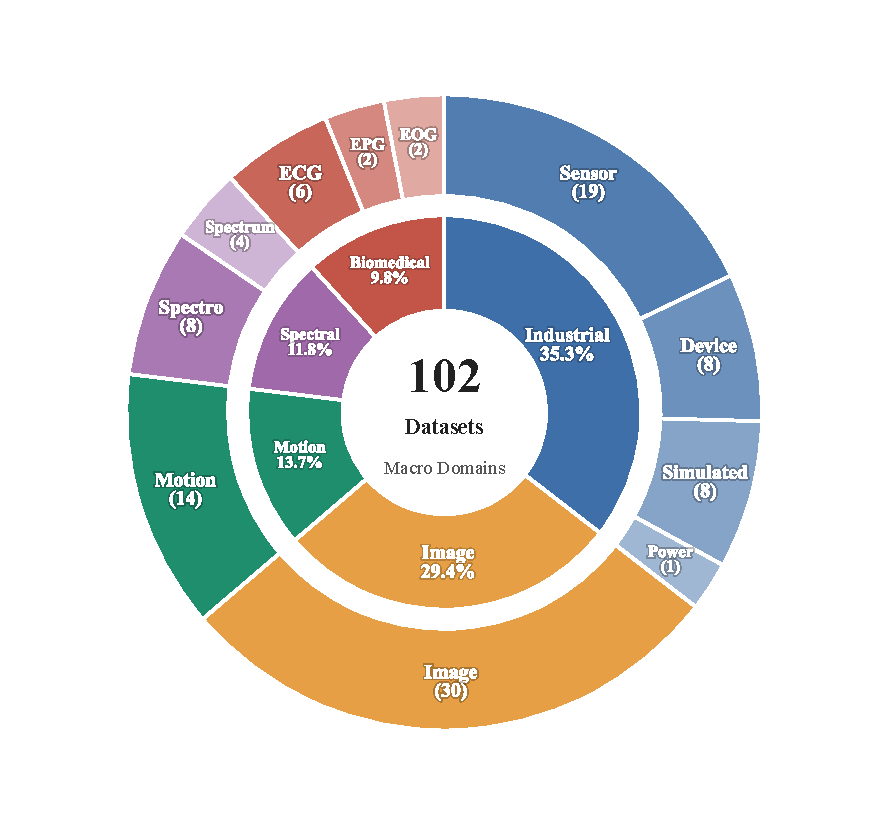
\includegraphics[trim=0cm 0cm 0cm 0cm,clip,width=.8\textwidth]{figures/fig_domain_coverage}
% \caption{Domain coverage of the 102 UCR datasets used in our
% experiments. Inner ring: the five macro-domains (true percentages
% shown). Outer ring: the 11 raw UCR categories with absolute counts.}
%   \label{fig:domain-coverage}
% \end{figure*}


\begin{figure}[H]
\centering
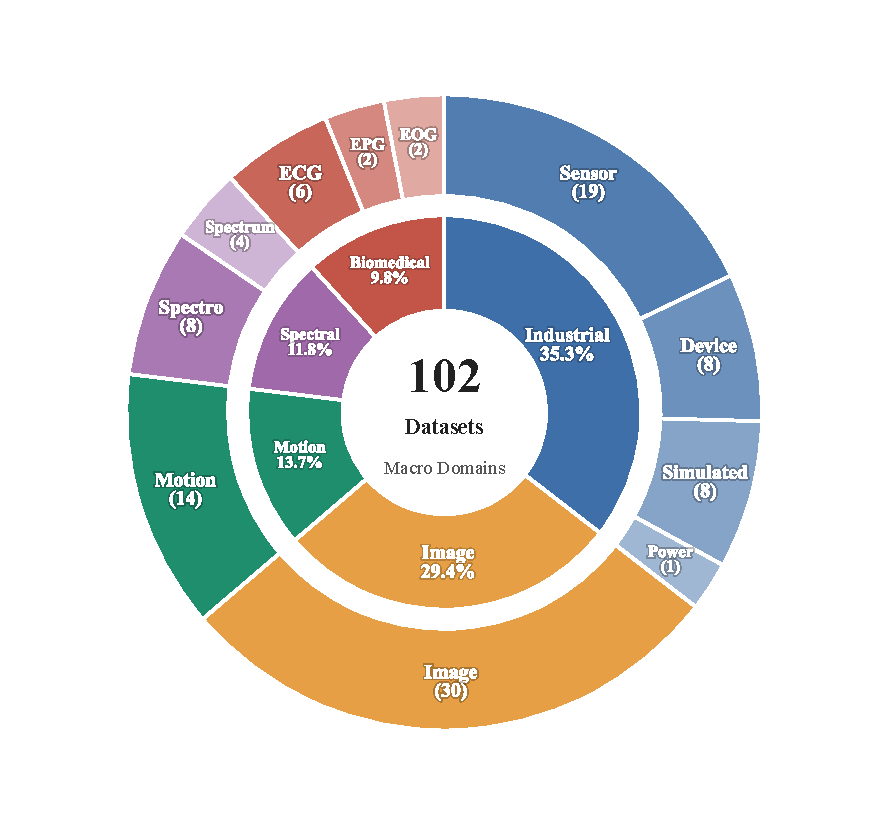
\includegraphics[width=.8\textwidth]{figures/fig_domain_coverage.pdf}
\caption{Domain coverage of the 102 UCR datasets used in our
experiments. Inner ring: the five macro-domains (true percentages
shown). Outer ring: the 11 raw UCR categories with absolute counts.}
\label{fig:domain-coverage}
\end{figure}

% ========== Extended related work discussion (TMLR rebuttal Q1) ==========
% ADDED FOR TMLR (rebuttal Q1)
\section{Extended related work discussion}
\label{app:related-extended}

% ADDED FOR TMLR (rebuttal Q1): full related-work discussion moved verbatim from sections/02_problem_setup.tex Section 2.2.
% Note: Figure~\ref{fig:SoTa} (images/SoTa_evolution_DA) remains in the main text Section 2.2 and is not duplicated here.
TS DA methods can be classified as traditional or
generative according to \citep{iglesias2023data, iwana2021empirical}
and summarised in Figure~\ref{fig:SoTa}.

\paragraph{Traditional DA methods}
Traditional DA methods, such as window slicing, jittering, and
scaling, are primarily adapted from
computer vision and rely on transformation strategies like
cropping, rotation, scaling, drifting, and so forth. However,
the complex nature of TS data often renders these
methods sub-optimal, as they can disrupt the semantic integrity
of the original data. For instance, while a slightly flipped
image of a cat remains recognisable, reversing the time axis of
an electrocardiogram sequence can render it meaningless. In
response to these challenges, more advanced DA techniques were
developed to automate the sequence of transformations to be
performed. The first method, named \textbf{AutoAugment (AA)}
\citep{cubuk2019autoaugment}, uses reinforcement learning to
explore transformation pipelines/policies. The second, named
\textbf{Fast AutoAugment (FAA)} \citep{lim2019fast}, uses
density matching as a faster search strategy, eliminating the
need for back-propagation. Subsequent methods, such as
\textbf{RandAugment} \citep{cubuk2020randaugment}, \textbf{Deep
AutoAugment} \citep{zheng_deep_2022}, and \textbf{Trivial
Augment} \citep{muller2021trivialaugment}, were introduced to
further simplify and refine the augmentation search strategy.
RandAugment streamlines the augmentation process by removing
the exhaustive search phase, instead applying a fixed number of
random transformations with adjustable magnitudes. Deep
AutoAugment incorporates a deep RL model that dynamically
combines transformation policies based on the specific
characteristics of the dataset. Trivial Augment introduces an
even simpler approach by applying a minimal set of random
transformations, emphasising ease of use and computational
efficiency. Despite these advancements, the aforementioned
methods rely on predefined transformations, which is suboptimal
for preserving intra-class consistency and the semantic
characteristics of the original TS data, thereby
limiting the effectiveness of DA.

\paragraph{Generative DA methods}
Generative DA models such as Generative Adversarial Networks (GANs) \citep{goodfellow2020generative},
diffusion models \citep{yang2023diffusion}, and VAEs
\citep{kingma2013auto} represent powerful techniques capable of
learning a probabilistic representation of data distributions.
These models can generate TS data that retain the
temporal dependencies, semantic consistency, and class-specific
characteristics of the original datasets \citep{fu2020data}. For
example, using a representation layer, as introduced by
\cite{liu2022learning}, provides an abstraction that is crucial
when dealing with TS data. \textbf{TimeGAN}
\citep{zhang2022data}, designed specifically for TS, shows
significant improvements in generating high-quality synthetic
sequences and augmenting low-quality datasets. Likewise, \textbf{TS-GAN} \citep{yang2023ts} develops
an LSTM-based GAN architecture with a
sequential-squeeze-and-excitation to better capture
time-dependence between the current and past moments in each
dimension. TS-GAN is proposed to generate augmented sensor-based
health data to improve Deep Learning classification models and
is evaluated on three health TS datasets.
\textbf{GT-GAN} \citep{jeon2022gt} introduces an invertible GAN
framework that combines controlled differential equations and
continuous-time flow processes, showing promising results.
\textbf{TTS-GAN} \citep{li2022tts} and its conditional variant
\textbf{TTS-cGAN} \citep{li2022ttsc} adapt the traditional GAN
architecture using a transformer-encoder architecture that can
deal with long-range dependencies in time sequences. They show
strong performance in generating realistic data across three
datasets: a simulated dataset, a human activity recognition
dataset, and an ECG dataset. \textbf{LatentAugment}
\citep{tronchin2023latentaugment} guides the latent space
learned by any GAN on the original data, applies noise-based
perturbations to the latent points, and decodes them to generate
new, semantically consistent samples. More recently,
\cite{seon2024least} proposed \textbf{LISGAN}, a GAN-based
architecture for TS augmentation under class
imbalance: they augment the loss with a mutual information term
and employ spectral normalisation. LISGAN yields high-quality
synthetic data and significantly improves classification
performance on industrial IoT datasets. A recent extension,
\textbf{TTS-WGAN-GP} \citep{mousavi2025transformer}, leverages
a transformer architecture within a Wasserstein GAN with gradient
penalty framework to improve DA quality for structural health
monitoring TS. However, training GANs is notoriously
unstable and highly sensitive to hyperparameter settings.
Without careful tuning, they often suffer from mode collapse,
which reduces sample diversity and leads to unrealistic data
distributions \citep{lei2019mode}.

Diffusion models generate
data by iteratively denoising noise toward the target
distribution, rather than via the adversarial training used by GANs. They have
achieved high-fidelity image generation (e.g., DALL$\cdot$E~2,
Imagen, Flux). Since 2023, several diffusion-based DA methods
for TS have appeared, including \textbf{SE-DDPM}
\citep{liu2024adaptive} for imbalanced TSC, \textbf{DiffRUL}
\citep{wang2024diffrul} for remaining useful life prediction,
\textbf{D3A-TS} \citep{solis2023} for meta-attribute
conditioning, \textbf{Time-DDPM} \citep{dai2023timeddpm} combining diffusion with
CNN-LSTM, \textbf{Diffusion-TS} \citep{yuandiffusion} with
seasonal-trend decomposition, and \textbf{ImagenTime}
\citep{naiman2024utilizing} transforming sequences into images.
\textbf{DiffAT} \citep{yu2025diffat} introduces a flexible
method that uses soft prompts distilled from traditional DA to
guide conditional diffusion for TS forecasting.
\textbf{Diff-TI} \citep{zhang2025time} proposes a hybrid
diffusion-transformer architecture where diffusion generates the
initial timestep (capturing the base distribution), followed by
iterative transformer prediction for the next timesteps.
Despite stable outputs, diffusion models still face challenges
with long-range dependencies, error accumulation, and slow
inference \citep{feng2024latent}, which can limit their
practical applications.

VAEs allow for explicit control over the
diversity of generated samples through manipulation
of the latent space, as evidenced by \cite{cheung2020modals}. Additionally, VAEs are
less prone to collapse compared to GANs and are less
computationally expensive than both GANs and diffusion models
\citep{thanh2020catastrophic}. The first VAE-based generative DA model relying on clustering,
named \textbf{VaDE}, was introduced by
\cite{jiang2016variational}. VaDE integrates a Gaussian Mixture
Model (GMM) as the prior distribution, jointly trained with the
encoder on unlabelled data, enabling realistic sample generation
for any specified cluster without supervised labels.
\textbf{GMVAE} \citep{dilokthanakul2017gmvae} similarly employs
a GMM-structured latent space to capture multi-modal data
distributions. In both cases, the mixture is an unsupervised
inductive bias: it is part of the generative model and appears
in the evidence lower bound (ELBO), and neither method provides a mechanism to control
the extent of generation beyond the learned distribution. \textbf{VAE-STS} \citep{goubeaud2021using} proposes a simple VAE
architecture for data generation. \textbf{KoVAE}
\citep{naiman2023generative} uses linear Koopman dynamics as a
prior, enabling interpretable and physics-constrained modelling
of both regular and irregular TS. \textbf{MODALS} was
introduced by \cite{cheung2020modals} and was the first study to
explore class boundary expansion during synthetic data
generation, though it lacks a mechanism to control the extent of
this expansion. Recently, \cite{dang2024vae} introduced
\textbf{VAE-LSTM} to augment an inertial sensor dataset with the
goal of enhancing classification performance. \textbf{Seq-MVAE}
\citep{bogojeski2025data} employs a VAE with multimodal
heterogeneous TS for industrial aging processes,
enabling DA that preserves cross-modal temporal dependencies.

However, none of these approaches explore a
progressive, tunable expansion of class representations in the
latent space, as proposed in ASCENSION.



% ========== Proof of Proposition 1 (TMLR addition) ==========
% Single chain of equalities computing Cov[Z] directly on d_y^alpha.
% One conceptual operation per line; large jumps from the earlier
% version split into atomic substitutions.
\section{Proof of Proposition~\ref{prop:variance}}
\label{app:variance-proof}

Let
$\mu_i = \mu_\phi(x_i)$ and $\Sigma_i = \Sigma_\phi(x_i)$
and
$\bar\mu_y = \tfrac{1}{|\mathcal{I}_y|}\sum_{i \in \mathcal{I}_y} \mu_i$ for compactness, we have:
\begin{align*}
\mathrm{Cov}_{Z \sim d_y^{\,\alpha}}[Z]
&= \mathbb{E}[Z\,Z^{\!\top}] - \mathbb{E}[Z]\,\mathbb{E}[Z]^{\!\top} \\[4pt]
&= \int z\,z^{\!\top}\,d_y^{\,\alpha}(z)\,\mathrm{d}z
 \;-\; \biggl(\int z\,d_y^{\,\alpha}(z)\,\mathrm{d}z\biggr)
       \biggl(\int z\,d_y^{\,\alpha}(z)\,\mathrm{d}z\biggr)^{\!\!\top} \\[4pt]
&= \int z\,z^{\!\top}\,\frac{1}{|\mathcal{I}_y|}\sum_{i \in \mathcal{I}_y}\mathcal{N}\!(z;\mu_i,\alpha\Sigma_i)\,\mathrm{d}z
   \;-\; \biggl(\int z\,\frac{1}{|\mathcal{I}_y|}\sum_{i \in \mathcal{I}_y}\mathcal{N}\!(z;\mu_i,\alpha\Sigma_i)\,\mathrm{d}z\biggr)
         \biggl(\int z\,\frac{1}{|\mathcal{I}_y|}\sum_{i \in \mathcal{I}_y}\mathcal{N}\!(z;\mu_i,\alpha\Sigma_i)\,\mathrm{d}z\biggr)^{\!\!\top} \\[4pt]
&= \frac{1}{|\mathcal{I}_y|}\sum_{i \in \mathcal{I}_y}
     \int z\,z^{\!\top}\,\mathcal{N}\!(z;\mu_i,\alpha\Sigma_i)\,\mathrm{d}z
   \;-\; \biggl(\frac{1}{|\mathcal{I}_y|}\sum_{i \in \mathcal{I}_y}
           \int z\,\mathcal{N}\!(z;\mu_i,\alpha\Sigma_i)\,\mathrm{d}z\biggr)
         \biggl(\frac{1}{|\mathcal{I}_y|}\sum_{i \in \mathcal{I}_y}
           \int z\,\mathcal{N}\!(z;\mu_i,\alpha\Sigma_i)\,\mathrm{d}z\biggr)^{\!\!\top} \\[4pt]
&= \frac{1}{|\mathcal{I}_y|}\sum_{i \in \mathcal{I}_y}
     \bigl[\,\alpha\Sigma_i + \mu_i\mu_i^{\!\top}\,\bigr]
   \;-\; \biggl(\frac{1}{|\mathcal{I}_y|}\sum_{i \in \mathcal{I}_y} \mu_i\biggr)
         \biggl(\frac{1}{|\mathcal{I}_y|}\sum_{i \in \mathcal{I}_y} \mu_i\biggr)^{\!\!\top}
   \quad\ \\[4pt]
&= \frac{1}{|\mathcal{I}_y|}\sum_{i \in \mathcal{I}_y}
     \bigl[\,\alpha\Sigma_i + \mu_i\mu_i^{\!\top}\,\bigr]
   \;-\; \bar\mu_y\,\bar\mu_y^{\!\top} \\[4pt]
&= \alpha\,\frac{1}{|\mathcal{I}_y|}\sum_{i \in \mathcal{I}_y} \Sigma_i
   \;+\; \frac{1}{|\mathcal{I}_y|}\sum_{i \in \mathcal{I}_y} \mu_i\,\mu_i^{\!\top}
   \;-\; \bar\mu_y\,\bar\mu_y^{\!\top} \\[4pt]
&= \alpha\,\frac{1}{|\mathcal{I}_y|}\sum_{i \in \mathcal{I}_y} \Sigma_i
   \;+\; \frac{1}{|\mathcal{I}_y|}\sum_{i \in \mathcal{I}_y}
         \bigl(\mu_i - \bar\mu_y\bigr)\bigl(\mu_i - \bar\mu_y\bigr)^{\!\top} \\[4pt]
&= \alpha\,\bar\Sigma_w(y) + \Sigma_b(y).
\end{align*}
\qed


% ========== cVAE baseline discussion (moved from §3.5) ==========
% -----------------------------------------------------------------
% ADDED FOR TMLR (review-driven) — cVAE baselines discussion.
% Previously sat in main text §3.5 ("Why not a class-conditional
% VAE?"); moved to appendix per the TMLR resubmission to keep §3
% focused on the method. The empirical comparison table is in
% Section~\ref{sec:results:cvae}.
% Source: Publication/ASCENSION/ASCENSION_Response_CVAEBaseline.md
% -----------------------------------------------------------------
\section{Comparison with class-conditional VAE baselines}
\label{app:cvae_baseline}
\label{sec:results:cvae}

A natural alternative to ASCENSION is a class-conditional VAE
(cVAE) that concatenates the class label to both encoder and
decoder inputs. To isolate the effect of ASCENSION's
contrastive clustering loss from the effect of class
conditioning, we evaluate three cVAE variants with ResNet and FCN on all 102 UCR
datasets: (i) the standard cVAE formulation with a fixed prior
$z \sim \mathcal{N}(0, I)$; (ii) a prior-scaled variant
$z \sim \mathcal{N}(0, \alpha\,I)$ with $\alpha > 1$ ($\alpha = 2.6)$; and (iii) cVAE generations refined with
ASCENSION's posterior-mixture sampling and filtering.
The single $\alpha = 2.6$ matches the value used for wall-clock
comparisons in Appendix~\ref{sec:complexity:wallclock}, the mean
of the per-dataset best $\alpha$ values across the 102 UCR datasets
(Tables~\ref{Tab:app:bestconfig:resnet}-\ref{Tab:app:bestconfig:moment}).
% REVISED FOR TMLR (rebuttal C1)
Variant (i) provides the no-scaling endpoint ($\alpha = 1$); variant
(iii) uses ASCENSION's per-dataset $\alpha$ values and therefore
covers the same $\alpha$ range as the best-configuration reference
(\tablename~\ref{tab:best-config}).
% ADDED FOR TMLR (rebuttal C6)
All three cVAE variants use the identical fully connected backbone as
ASCENSION (Section~\ref{sec:method:vae}), with the one-hot class label
concatenated to both the encoder and the decoder inputs.

\begin{table}[H]
\centering
\caption{ASCENSION vs.\ three cVAE variants (no contrastive loss)
on 102 UCR datasets.}
\label{tab:cvae}
\resizebox{\textwidth}{!}{%
\begin{tabular}{@{}llrrrrrrrrrr@{}}
\toprule
 & \multirow{2}{*}{\bf DA method}
  & \multicolumn{2}{c}{\bf Improved}
  & \multicolumn{2}{c}{\bf Unchanged}
  & \multicolumn{2}{c}{\bf Worsened}
  & \multicolumn{2}{c}{\bf Total} \\
 & 
  & $\uparrow$Nb$_{\text{data}}$ & $\uparrow\overline{\Delta\mathrm{Acc}}$
  & Nb$_{\text{data}}$ & $\overline{\Delta\mathrm{Acc}}$
  & $\downarrow$Nb$_{\text{data}}$ & $\downarrow\overline{\Delta\mathrm{Acc}}$
  & Nb$_{\text{data}}$ & $\overline{\Delta\mathrm{Acc}}$ \\
\midrule
\multirow{4}{*}{\rotatebox{90}{ResNet}}
  & cVAE prior, $\mathcal{N}(0, I)$       & 32 & 3.9\% & 17 & 0\% & 53 & -2.3\% & 102 & $+0.05\%$ \\
  & cVAE prior, $\mathcal{N}(0, 2.6\,I)$ & 36 & 1.8\% & 12 & 0\% & 54 & -2.7\% & 102 & $-0.76\%$ \\
  & cVAE + posterior mixture              & 42 & 2.0\% & 15 & 0\% & 45 & -1.7\% & 102 & $+0.09\%$ \\
  & \textbf{ASCENSION}                    & \textbf{59} & \textbf{4.1\%} & 16 & 0\% & \textbf{27} & \textbf{-1.9\%} & 102 & $\mathbf{+1.9\%}$ \\
\midrule
\multirow{4}{*}{\rotatebox{90}{FCN}}
  & cVAE prior, $\mathcal{N}(0, I)$       & 32 & 2.5\% & 15 & 0\% & 55 & -2.7\% & 102 & $-0.68\%$ \\
  & cVAE prior, $\mathcal{N}(0, 2.6\,I)$ & 25 & 2.5\% & 13 & 0\% & 64 & -3.2\% & 102 & $-1.38\%$ \\
  & cVAE + posterior mixture              & 42 & 1.9\% & 14 & 0\% & 46 & -2.5\% & 102 & $-0.32\%$ \\
  & \textbf{ASCENSION}                    & \textbf{56} & \textbf{4.0\%} & 12 & 0\% & \textbf{34} & \textbf{-2.5\%} & 102 & $\mathbf{+1.4\%}$ \\
\bottomrule
\end{tabular}%
}
\end{table}

\paragraph{Why label conditioning is not enough?}
The cVAE benefits from label conditioning, but frequently
produces overlapping latent regions for classes with similar
temporal patterns, which leads to degraded performance on roughly
half of the datasets across all three variants ($53$/$54$/$45$
with ResNet and $55$/$64$/$46$ with FCN, for the standard prior,
prior-scaled, and posterior-mixture variants respectively).
ASCENSION's margin-based contrastive
loss actively pushes classes apart, enlarging the Bayes regions
$\mathcal{R}_y^{\,\alpha}$ (Definition~\ref{def:bayes-region})
that the $\alpha$-scaling mechanism populates. The contrastive
loss is therefore not merely an alternative to label conditioning
but an essential component of the method (cf Proposition~\ref{prop:variance}  and
Section~\ref{sec:analysis:ablation},
\tablename~\ref{tab:ablation}, where removing $\mathcal{L}_{\text{cluster}}$
collapses the mean augmentation gain from $+2.1\%$ to $-0.05\%$).



% ========== Best per-dataset configuration reference results ==========
% -----------------------------------------------------------------
% REVISED FOR TMLR (rebuttal C1)
% The former "Single-configuration reference results" section became
% redundant once the fixed-configuration comparison took over the
% main-text \tablename~\ref{tab:main-results}. This section now hosts
% the originally submitted Table 1 (ASCENSION at its best per-dataset
% configuration), moved here verbatim from Section 4 with its label
% changed to tab:best-config.
% -----------------------------------------------------------------
\section{Best per-dataset configuration reference results}
\label{app:best-config}
\label{app:single-config}% kept so stale references keep resolving

This reference follows the protocol of \tablename~1 in the originally
submitted version: \tablename~\ref{tab:best-config} reports ASCENSION
at its best hyperparameter configuration per dataset, with baselines at
their authors' recommended defaults, in a single run. The
feature-importance analysis of Figure~\ref{fig:catch22-importance}
was built on these runs, while the discrepancy-axis analysis of
Figure~\ref{fig:cumsum-disc} is computed on the fixed-configuration
runs. Per-dataset selection widens ASCENSION's margins
relative to the fixed configuration of
\tablename~\ref{tab:main-results}, with net totals of $+1.9\%$,
$+1.4\%$ and $+2.4\%$ on ResNet, FCN and Moment, and ASCENSION remains
the only method with a positive net total on every classifier.

\begin{table}[H]
\centering

\caption{For each DA method, we show the number of datasets (Nb$_{\text{data}}$), \emph{out of 102}, with improved, unchanged, or worsened accuracy, plus the mean accuracy change $\overline{\Delta\mathrm{Acc}} = \mathrm{augmentation\_accuracy} - \mathrm{base\_accuracy}$ averaged over each subset. Arrows $(\uparrow, \downarrow)$ mark direction of improvement; \textbf{bold} and \underline{underline} indicate \textbf{best} and \underline{second best}.}
\label{tab:best-config}
\resizebox{\textwidth}{!}{%
\begin{tabular}{@{}llrrrrrrrrrr@{}}
\toprule
 & \multirow{2}{*}{\bf DA method} & \multirow{2}{*}{\bf (Venue, Year)}
  & \multicolumn{2}{c}{\bf Improved}
  & \multicolumn{2}{c}{\bf Unchanged}
  & \multicolumn{2}{c}{\bf Worsened}
  & \multicolumn{2}{c}{\bf Total} \\
  & &
  & $\uparrow$Nb$_{\text{data}}$ & $\uparrow\overline{\Delta\mathrm{Acc}}$
  & Nb$_{\text{data}}$ & $\overline{\Delta\mathrm{Acc}}$
  & $\downarrow$Nb$_{\text{data}}$ & $\downarrow\overline{\Delta\mathrm{Acc}}$
  & Nb$_{\text{data}}$ & $\overline{\Delta\mathrm{Acc}}$ \\
\midrule
\multirow{9}{*}{\rotatebox{90}{ResNet}}
 & VaDE       &  (IJCAI, 2016)     & \underline{44} & 2.8\%  & 9  & 0\% & 49 & -7.1\%  & 102  & $-2.2\%$ \\
 & FAA        &  (NeurIPS, 2019)   & 19 & \underline{7.8\%} & 8  & 0\% & 75 & -9.2\%  & 102  & $-5.3\%$ \\
 & TTS-GAN     & (AIME, 2022)      & 26 & 2.2\%  & 11 & 0\% & 65 & -8.3\%  & 102  & $-4.7\%$ \\
 & KoVAE      &  (ICLR, 2024)      & 38 & 1.5\%  & 19 & 0\% & \underline{45} & \underline{-2.1\%} & 102 & $\underline{-0.4\%}$ \\
 & Time-DDPM   & (SENS.\,J., 2023) & 38 & \textbf{16.3\%} & 0  & 0\% & 64 & -22.3\% & 102 & $-7.9\%$ \\
 & LA         &  (ArXiv, 2023)     & 14 & 3.3\%  & 13 & 0\% & 75 & -3.9\%  & 102  & $-2.4\%$ \\
 & ImagenTime  & (NeurIPS, 2024)   & 15 & 1.3\%  & 13 & 0\% & 74 & -6.1\%  & 102  & $-4.2\%$ \\
 & Diffusion-TS &(ICLR, 2024)      & 21 & 1.3\%  & 5  & 0\% & 76 & -9.3\%  & 102  & $-6.7\%$ \\
 & \textbf{ASCENSION} &            & \textbf{59} & 4.1\%
                                   & 16 & 0\% & \textbf{27} & \textbf{-1.9\%} & 102 & $\mathbf{+1.9\%}$ \\
\midrule
\multirow{9}{*}{\rotatebox{90}{FCN}}
 & VaDE    &     (IJCAI, 2016)     & 42 & 3.4\%  & 15 & 0\% & 45 & -7.0\%  & 102  & $-1.7\%$ \\
 & FAA      &    (NeurIPS, 2019)   & 14 & \underline{7.1\%} & 3  & 0\% & 85 & -15.0\% & 102 & $-11.5\%$ \\
 & TTS-GAN  &    (AIME, 2022)      & 36 & 2.9\%  & 17 & 0\% & 49 & -8.2\%  & 102  & $-2.9\%$ \\
 & KoVAE    &    (ICLR, 2024)      & 41 & 2.1\%  & 15 & 0\% & 46 & \textbf{-2.1\%} & 102 & $-0.1\%$ \\
 & Time-DDPM   & (SENS.\,J., 2023) & 42 & \textbf{16.9\%} & 1  & 0\% & 59 & -23.0\% & 102 & $-6.3\%$ \\
 & LA       &    (ArXiv, 2023)     & \underline{44} & 2.3\%  & 19 & 0\% & \underline{39} & \underline{-2.6\%} & 102 & $\underline{0.0\%}$ \\
 & ImagenTime  & (NeurIPS, 2024)   & 38 & 2.7\%  & 11 & 0\% & 53 & -2.9\%  & 102  & $-0.5\%$ \\
 & Diffusion-TS &(ICLR, 2024)      & 36 & 3.3\%  & 7  & 0\% & 59 & -13.5\% & 102 & $-6.6\%$ \\
 & \textbf{ASCENSION}   &          & \textbf{56} & 4.0\%
                                   & 12 & 0\% & \textbf{34} & -2.5\% & 102 & $\mathbf{+1.4\%}$ \\
\midrule
\multirow{9}{*}{\rotatebox{90}{Moment}}
 & VaDE   &      (IJCAI, 2016)     & 35 & 2.9\%  & 8  & 0\% & 59 & -5.6\%  & 102  & $-2.2\%$ \\
 & FAA    &      (NeurIPS, 2019)   & \underline{50} & \textbf{7.8\%} & 6  & 0\% & \underline{46} & -11.8\% & 102 & $-1.5\%$ \\
 & TTS-GAN  &    (AIME, 2022)      & 41 & 3.4\%  & 7  & 0\% & 54 & \underline{-5.2\%} & 102 & $\underline{-1.4\%}$ \\
 & KoVAE    &    (ICLR, 2024)      & 27 & 3.7\%  & 5  & 0\% & 70 & -12.2\% & 102 & $-7.4\%$ \\
 & Time-DDPM &   (SENS.\,J., 2023) & 35 & 3.8\%  & 5  & 0\% & 62 & -7.0\%  & 102  & $-2.9\%$ \\
 & LA      &     (ArXiv, 2023)     & 31 & 2.6\%  & 6  & 0\% & 65 & -5.5\%  & 102  & $-2.7\%$ \\
 & ImagenTime  & (NeurIPS, 2024)   & 25 & 2.1\%  & 7  & 0\% & 70 & -6.3\%  & 102  & $-3.8\%$ \\
 & Diffusion-TS &(ICLR, 2024)      & 28 & 3.2\%  & 5  & 0\% & 69 & -8.8\%  & 102  & $-5.1\%$ \\
 & \textbf{ASCENSION}   &          & \textbf{72} & 3.8\%
                                   & 10 & 0\% & \textbf{20} & \textbf{-1.6\%} & 102 & $\mathbf{+2.4\%}$ \\
\bottomrule
\end{tabular}%
}
\end{table}




% ========== Statistical significance (Friedman + CD diagrams) ==========
% REVISED FOR TMLR (rebuttal C3)
\section{Statistical significance on the best-configuration reference}
\label{app:cd}

The critical-difference (CD) analysis of the fixed-configuration
results now appears in the main text
(Section~\ref{sec:results:significance}). As its best-configuration
companion, this section reports the same analysis computed on the
best-per-dataset configuration reference of
Appendix~\ref{app:best-config} (\tablename~\ref{tab:best-config},
single run). We report Friedman tests and CD diagrams (Nemenyi
post-hoc at the $5\%$ significance level)
following~\citep{demsar2006statistical}, computed over per-dataset
accuracies for each of the three classifiers. The Friedman test
rejects the null hypothesis that all DA methods perform equally with
$p < 10^{-18}$ on every classifier, and the critical-difference
threshold for $k = 9$ methods and $N = 102$ datasets is
$\mathrm{CD} \approx 1.19$.
Figures~\ref{fig:cd-resnet}, \ref{fig:cd-fcn}, and~\ref{fig:cd-moment}
show the resulting CD diagrams for ResNet, FCN, and Moment respectively.

\begin{figure}[H]
\centering
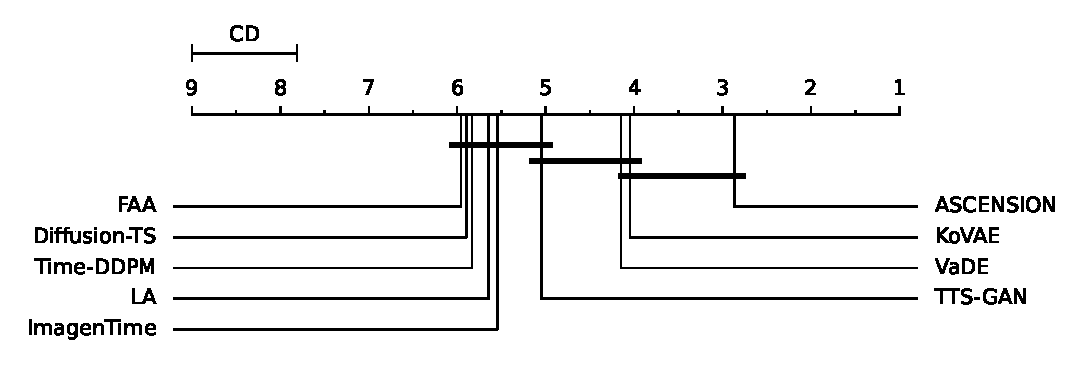
\includegraphics[width=0.85\linewidth]{figures/cd_diagram_resnet.pdf}
% REVISED FOR TMLR (rebuttal C3)
\caption{Critical-difference diagram, ResNet classifier (Friedman + Nemenyi at the $5\%$ significance level), computed on the best-per-dataset configuration reference of \tablename~\ref{tab:best-config}, single run.}
\label{fig:cd-resnet}
\end{figure}

\begin{figure}[H]
\centering
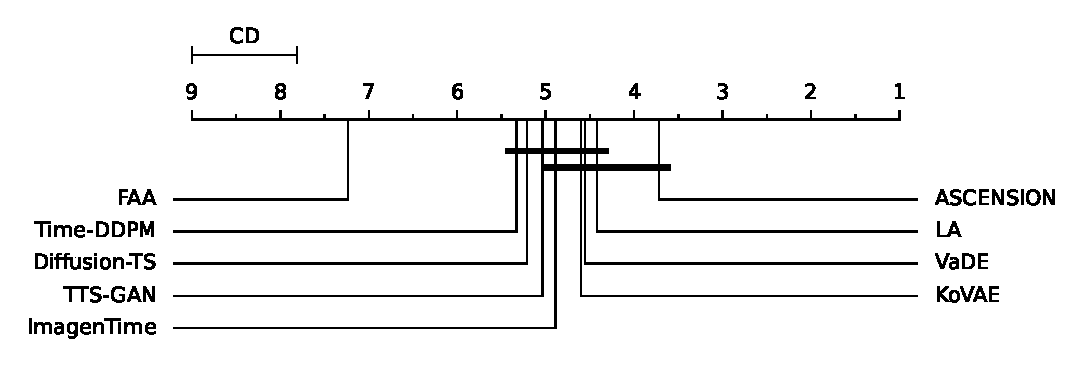
\includegraphics[width=0.85\linewidth]{figures/cd_diagram_fcn.pdf}
% REVISED FOR TMLR (rebuttal C3)
\caption{Critical-difference diagram, FCN classifier (Friedman + Nemenyi at the $5\%$ significance level), computed on the best-per-dataset configuration reference of \tablename~\ref{tab:best-config}, single run.}
\label{fig:cd-fcn}
\end{figure}

\begin{figure}[H]
\centering
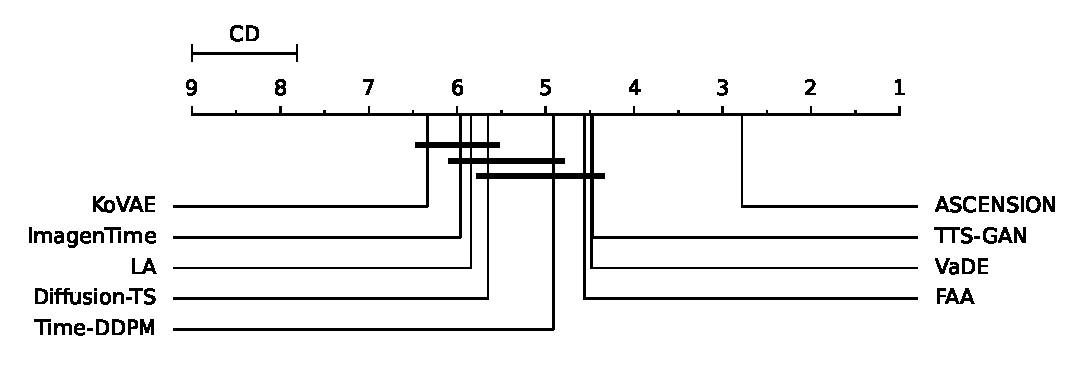
\includegraphics[width=0.85\linewidth]{figures/cd_diagram_moment.pdf}
% REVISED FOR TMLR (rebuttal C3)
\caption{Critical-difference diagram, Moment classifier (Friedman + Nemenyi at the $5\%$ significance level), computed on the best-per-dataset configuration reference of \tablename~\ref{tab:best-config}, single run.}
\label{fig:cd-moment}
\end{figure}

% REVISED FOR TMLR (rebuttal C3)
On this best-configuration reference, ASCENSION achieves the lowest
mean rank on every classifier (2.87, 3.72, 2.79 for ResNet, FCN,
Moment), consistent with the fixed-configuration analysis of
Section~\ref{sec:results:significance}. On the Moment
classifier the Nemenyi post-hoc places ASCENSION significantly
ahead of every other DA method. On ResNet, ASCENSION is
significantly better than all baselines except KoVAE, whose
rank gap to ASCENSION ($1.18$) is just inside the critical
distance. On FCN, ASCENSION is significantly better than FAA,
Time-DDPM, Diffusion-TS, and TTS-GAN; the remaining baselines
(KoVAE, LA, VaDE, ImagenTime) occupy a shared rank band with
ASCENSION at its lower edge.



% ========== Per-dataset variability across runs (TMLR rebuttal C4) ==========
% ADDED FOR TMLR (rebuttal C4)
\section{Per-dataset variability across runs}
\label{app:per-dataset-std}

\tablename~\ref{tab:per-dataset-std} reports, for every dataset, the
standard deviation of the ASCENSION gain across the three
fixed-configuration runs of \tablename~\ref{tab:main-results}. The
median standard deviation is $1.6$ accuracy points on ResNet, $1.6$ on
FCN and $2.1$ on Moment, with maxima of $18.6$, $19.8$ and $10.4$
respectively. The Moment classification stage is deterministic, so its
per-dataset variability comes from the generation stage alone.

\begin{table}[H]
\centering
\caption{Per-dataset standard deviation (accuracy points) of the ASCENSION
gain across the three fixed-configuration runs. The median is
1.6 on ResNet, 1.6 on FCN and 2.1 on Moment, with maxima of
18.6, 19.8 and 10.4 respectively, which motivates reporting
distributions and ranks rather than single per-dataset values.}
\label{tab:per-dataset-std}
\resizebox{\textwidth}{!}{%
\begin{tabular}{@{}lrrr@{\hspace{2em}}lrrr@{}}
\toprule
\bf Dataset & ResNet & FCN & Moment & \bf Dataset & ResNet & FCN & Moment \\
\midrule
ACSF1 & 3.5 & 2.6 & 3.2 & Meat & 1.0 & 2.5 & 3.8 \\
Adiac & 2.3 & 4.1 & 4.7 & MedicalImages & 0.8 & 1.2 & 3.5 \\
ArrowHead & 3.0 & 0.9 & 3.8 & MiddlePhalanxOutlineAgeGroup & 1.5 & 0.4 & 4.3 \\
BME & 1.7 & 11.2 & 5.6 & MiddlePhalanxOutlineCorrect & 2.8 & 1.0 & 1.2 \\
Beef & 7.7 & 11.5 & 0.0 & MiddlePhalanxTW & 2.0 & 1.7 & 2.1 \\
BeetleFly & 2.9 & 2.9 & 2.9 & MixedShapesRegularTrain & 1.3 & 1.0 & 2.3 \\
BirdChicken & 8.7 & 10.0 & 2.9 & MixedShapesSmallTrain & 1.3 & 2.0 & 3.8 \\
CBF & 0.2 & 0.5 & 3.3 & MoteStrain & 2.1 & 0.5 & 2.5 \\
Car & 4.2 & 1.7 & 1.0 & NonInvasiveFetalECGThorax1 & 3.4 & 9.0 & 3.4 \\
ChlorineConcentration & 2.3 & 0.7 & 8.6 & NonInvasiveFetalECGThorax2 & 2.8 & 6.5 & 1.6 \\
CinCECGTorso & 2.8 & 4.2 & 1.8 & OSULeaf & 3.7 & 3.4 & 1.7 \\
Coffee & 2.1 & 2.1 & 2.1 & OliveOil & 3.3 & 5.1 & 3.8 \\
Computers & 5.5 & 8.7 & 2.6 & PhalangesOutlinesCorrect & 1.5 & 1.0 & 0.8 \\
Crop & 1.2 & 0.8 & 1.5 & Plane & 0.0 & 0.0 & 0.5 \\
DistalPhalanxOutlineAgeGroup & 1.4 & 5.4 & 1.9 & PowerCons & 0.3 & 1.7 & 5.3 \\
DistalPhalanxOutlineCorrect & 0.8 & 0.7 & 2.4 & ProximalPhalanxOutlineAgeGroup & 0.3 & 0.7 & 0.6 \\
DistalPhalanxTW & 2.9 & 0.8 & 2.3 & ProximalPhalanxOutlineCorrect & 1.2 & 1.3 & 1.4 \\
ECG200 & 5.2 & 0.6 & 1.2 & ProximalPhalanxTW & 1.3 & 0.8 & 1.0 \\
ECG5000 & 0.1 & 0.1 & 0.4 & RefrigerationDevices & 1.0 & 0.8 & 2.5 \\
ECGFiveDays & 3.4 & 4.6 & 4.2 & Rock & 9.2 & 3.1 & 6.1 \\
EOGHorizontalSignal & 0.4 & 4.0 & 4.9 & ScreenType & 1.1 & 4.0 & 1.1 \\
EOGVerticalSignal & 2.5 & 3.1 & 5.4 & SemgHandGenderCh2 & 1.7 & 2.7 & 1.7 \\
Earthquakes & 0.8 & 1.9 & 0.4 & SemgHandMovementCh2 & 5.4 & 3.0 & 3.2 \\
ElectricDevices & 1.3 & 0.3 & 2.8 & SemgHandSubjectCh2 & 1.1 & 5.0 & 2.2 \\
EthanolLevel & 18.6 & 19.8 & 3.2 & ShapeletSim & 2.0 & 0.6 & 3.1 \\
FaceAll & 10.1 & 0.6 & 4.6 & ShapesAll & 2.8 & 5.2 & 1.4 \\
FaceFour & 2.4 & 3.0 & 5.7 & SmallKitchenAppliances & 1.9 & 1.8 & 1.7 \\
FacesUCR & 3.1 & 1.2 & 5.7 & SmoothSubspace & 0.0 & 0.4 & 2.8 \\
Fish & 6.0 & 6.3 & 0.3 & SonyAIBORobotSurface1 & 1.4 & 0.3 & 10.4 \\
FordA & 0.3 & 0.2 & 0.3 & SonyAIBORobotSurface2 & 1.5 & 0.7 & 1.1 \\
FordB & 2.1 & 0.5 & 1.0 & StarLightCurves & 0.2 & 0.9 & 2.4 \\
FreezerRegularTrain & 0.0 & 0.2 & 1.1 & Strawberry & 1.1 & 0.7 & 0.5 \\
FreezerSmallTrain & 3.7 & 1.8 & 2.9 & SwedishLeaf & 1.3 & 1.1 & 1.4 \\
GunPoint & 2.0 & 2.3 & 3.2 & Symbols & 2.7 & 12.8 & 1.4 \\
GunPointAgeSpan & 0.2 & 1.3 & 1.1 & SyntheticControl & 0.2 & 0.2 & 1.8 \\
GunPointMaleVersusFemale & 0.4 & 0.9 & 0.2 & ToeSegmentation1 & 0.9 & 0.9 & 1.2 \\
GunPointOldVersusYoung & 0.0 & 0.0 & 0.3 & ToeSegmentation2 & 1.2 & 0.8 & 5.2 \\
Ham & 1.0 & 1.0 & 1.1 & Trace & 0.6 & 0.0 & 2.3 \\
HandOutlines & 0.4 & 2.0 & 0.9 & TwoLeadECG & 2.6 & 3.3 & 5.3 \\
Haptics & 2.8 & 3.6 & 2.9 & TwoPatterns & 1.2 & 0.3 & 0.1 \\
Herring & 4.1 & 0.9 & 1.6 & UMD & 6.7 & 3.5 & 3.7 \\
HouseTwenty & 1.9 & 0.8 & 1.0 & UWaveGestureLibraryAll & 1.1 & 3.7 & 1.0 \\
InlineSkate & 3.7 & 4.0 & 3.0 & UWaveGestureLibraryX & 0.1 & 0.3 & 1.0 \\
InsectEPGRegularTrain & 0.0 & 0.0 & 1.5 & UWaveGestureLibraryY & 1.5 & 1.8 & 1.3 \\
InsectEPGSmallTrain & 0.0 & 0.0 & 5.4 & UWaveGestureLibraryZ & 0.8 & 0.4 & 0.7 \\
InsectWingbeatSound & 1.8 & 0.7 & 0.8 & Wafer & 0.0 & 0.1 & 0.1 \\
ItalyPowerDemand & 0.6 & 0.1 & 2.4 & Wine & 8.6 & 4.3 & 5.7 \\
LargeKitchenAppliances & 0.7 & 3.4 & 2.1 & WordSynonyms & 1.5 & 3.5 & 2.0 \\
Lightning2 & 1.6 & 1.6 & 1.6 & Worms & 6.9 & 4.2 & 0.0 \\
Lightning7 & 3.6 & 2.4 & 2.9 & WormsTwoClass & 3.0 & 1.5 & 1.5 \\
Mallat & 1.4 & 9.7 & 3.7 & Yoga & 3.6 & 1.8 & 0.5 \\
\bottomrule
\end{tabular}%
}
\end{table}


% ========== Moment classifier specification (TMLR rebuttal C5/WS9) ==========
% ADDED FOR TMLR (rebuttal C5/WS9)
\section{Moment classifier specification}
\label{app:moment-spec}

We use the frozen MOMENT-1-large encoder in embedding mode, feeding
each series to the encoder as a single channel and extracting the
mean-reduced 1024-dimensional embedding. The classifier is a
scikit-learn pipeline that applies feature standardisation followed by
an SVC (RBF kernel, $C = 1.0$, class-balanced weights). We fit the
pipeline independently on the original samples only and on the
original plus synthetic samples, and we evaluate both fits on the same
test set. No epoch-based selection is involved. This setting tests
augmentation when the classifier is a frozen foundation-model encoder
with a shallow head: synthetic samples cannot reshape the learned
features and can only move the decision boundary.


% ========== Gain against training-set size (TMLR rebuttal WS8) ==========
% ADDED FOR TMLR (rebuttal WS8)
\section{Gain against training-set size}
\label{app:gain-vs-spc}

Figure~\ref{fig:gain-vs-spc} plots the per-dataset ASCENSION gain
against the number of training samples per class. It complements the
applicability profile of Section~\ref{sec:results:applicability}.

\begin{figure}[H]
\centering
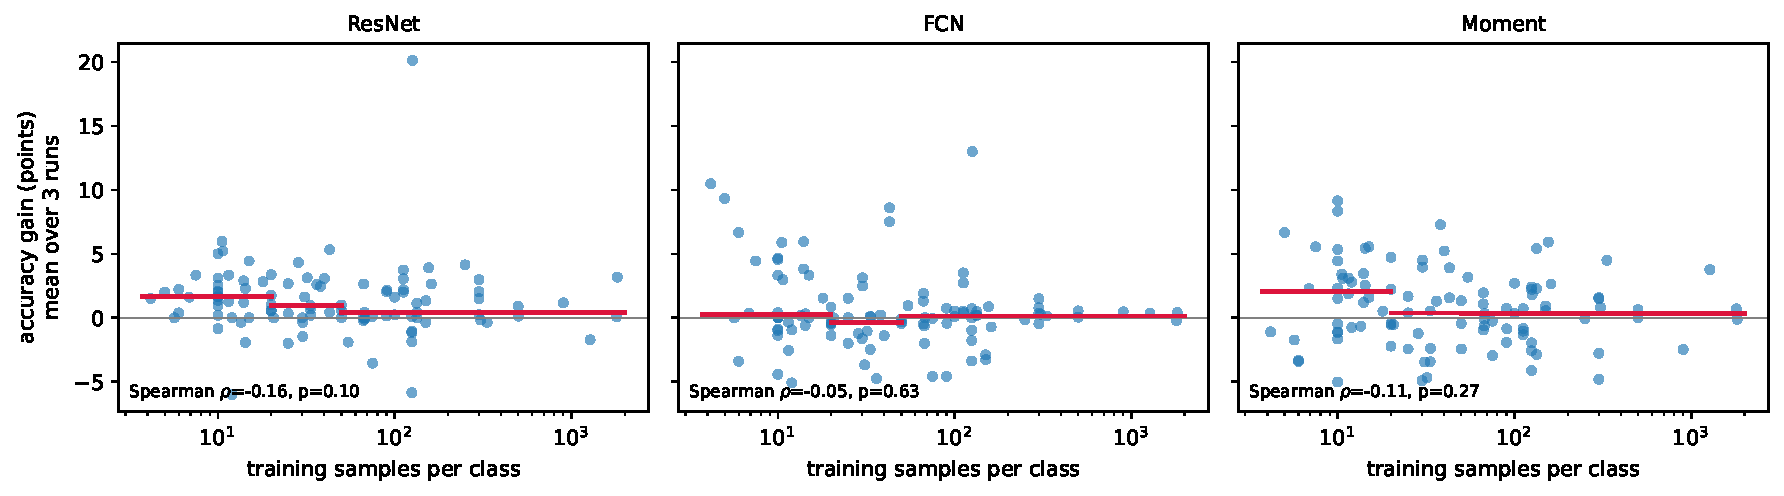
\includegraphics[width=0.9\linewidth]{figures/gain_vs_samples_per_class.pdf}
\caption{Per-dataset ASCENSION gain, averaged over the three
fixed-configuration runs, against the number of training samples per
class (log scale). Red markers show the group medians, and each panel
reports the per-classifier Spearman correlation.}
\label{fig:gain-vs-spc}
\end{figure}


% ========== Empirical acceptance rate across iterations =========

% =====================================================================
% ADDED FOR TMLR (additional analysis) — protocol details for the
% validation-selected iteration count of Section sec:results:valselect.
% =====================================================================
\section{Validation-selected iteration count: protocol details}
\label{app:valselect}

This appendix details the sealed protocol of
Section~\ref{sec:results:valselect}.

\paragraph{Cohort}
The 78 datasets are the UCR 2018 datasets whose training sets admit a
stratified internal validation fold, defined by two criteria computed
from training labels only: the smallest class holds at least 10
samples and the training set holds at least 30 samples. Seventy-five
of them belong to the 102 datasets of the main comparison. The three
Cricket datasets (CricketX, CricketY, CricketZ) meet the criteria but
were not part of the original campaign, and we keep them for cohort
completeness.

\paragraph{Ladder and selection rule}
For each dataset and seed, the training set is split once into a fit
fold and a validation fold. Synthetic candidates are anchored on the
fit fold only. The ladder evaluates $t \in \{0, 1, 2, 4, 8\}$
cumulative augmentation iterations. At each iteration, candidates are
drawn with the one-to-one budget of Algorithm~\ref{alg:ascension},
decoded, and filtered by the Bayes-region test. Two implementation
choices matter for the sealed setting. First, each iteration retrains
the VAE from scratch on the union of the real fit fold and all
previously accepted synthetic samples, so the expansion compounds as
described in Section~\ref{sec:method}. Second, the Bayes-region filter
is evaluated by a fixed verifier, a VAE trained once on the real fit
fold only. Candidates decoded by the current VAE are re-encoded by the
verifier and must pass the test against its real-only class mixtures.
This prevents the acceptance region from drifting as synthetic data
accumulates over iterations. One classifier is trained per rung, with
early stopping on the validation fold, and the test set is scored once
per rung and consulted only after $t^{*}$ is fixed. The deployed rung
maximises validation accuracy, ties are broken by validation
cross-entropy, remaining ties by the smaller $t$. At $t^{*} = 0$ the
deployed model is the unaugmented baseline itself, so a rejection can
never cost accuracy relative to not augmenting.

\paragraph{Strata}
Two strata were pre-declared from training labels before execution
(per-stratum results in \tablename~\ref{tab:valselect-strata}):
small-$n$ (training set of at most 60 samples, 11 datasets: ArrowHead,
BME, Car, GunPoint, HouseTwenty, Lightning2, Meat, ToeSegmentation1,
ToeSegmentation2, UMD, Wine) and imbalanced (at most 3 classes and
imbalance ratio at least 2.5, 8 datasets, evaluated in balanced
accuracy). The remaining 59 datasets form the third stratum.

\begin{table}[H]
\centering
\caption{Deployed gain per stratum (accuracy points, balanced accuracy
for the imbalanced stratum), with cell-level $t$ statistics and cell
counts. 3 seeds per dataset.}
\label{tab:valselect-strata}
\begin{tabular}{@{}lccc@{}}
\toprule
\bf Stratum & \bf ResNet & \bf FCN & \bf InceptionTime \\
\midrule
All cells ($n=234$)            & $+0.53$ $(t=1.83)$ & $+0.89$ $(t=2.95)$ & $+0.73$ $(t=2.66)$ \\
Small-$n$ ($n=33$)             & $+2.72$ $(t=2.59)$ & $+3.50$ $(t=2.59)$ & $-0.12$ $(t=-0.27)$ \\
Imbalanced, bal.\ acc.\ ($n=24$) & $-0.39$ $(t=-0.43)$ & $-0.21$ $(t=-0.53)$ & $-0.68$ $(t=-0.93)$ \\
Remaining ($n=177$)            & $+0.07$ $(t=0.23)$ & $+0.57$ $(t=1.94)$ & $+0.97$ $(t=2.80)$ \\
Abstention ($t^{*}=0$)         & $49\%$ & $48\%$ & $46\%$ \\
\bottomrule
\end{tabular}
\end{table}

\paragraph{Reading}
No stratum is systematically harmed under any classifier, every
negative stratum mean sits within noise. The imbalanced stratum is
dominated by datasets whose baselines are already near ceiling (Wafer,
StarLightCurves), where the rule can only abstain or misfire, and its
mean stays within noise for all three classifiers. The small-$n$
gains appear for the two classifiers whose small-$n$ baselines are
weakest and vanish for InceptionTime, whose architecture already
extracts on 30 to 60 series what augmentation supplies to the weaker
judges. The engaged cells use the whole ladder (on ResNet, 41/29/32/18
cells at $t = 1/2/4/8$), so the per-dataset dosage is real rather than
a constant choice. These observations about baseline headroom are
post-hoc readings of pre-registered endpoints, and we label them as
such.

\section{Empirical acceptance rate of the rejection step}
\label{app:acceptance}

As a robustness check we measure, for each augmentation iteration
$k$, the empirical acceptance rate
\begin{equation}
\mathcal{C}_y^{\,k}
= \mathbb{P}_{Z \sim d_y^{\,\alpha^k}}\!\left[
    \arg\max_{y'} d_{y'}^{\,\alpha^k}(Z) = y
  \right],
\label{eq:confidence}
\end{equation}
i.e.\ the fraction of $\alpha^k$-scaled samples that the
likelihood-dominance rule classifies into the originating class
$y$. This is the empirical counterpart of the acceptance rate
plotted in Figure~\ref{fig:prop1-heatmap}: same quantity, real
encoded UCR data instead of an analytic Gaussian model. We
estimate $\mathcal{C}_y^{\,k}$ by sampling $n=1000$ latents per
class.

\begin{figure}[H]
\centering
\resizebox{0.75\textwidth}{!}{% GNUPLOT: LaTeX picture with Postscript
\begingroup
  \makeatletter
  \providecommand\color[2][]{%
    \GenericError{(gnuplot) \space\space\space\@spaces}{%
      Package color not loaded in conjunction with
      terminal option `colourtext'%
    }{See the gnuplot documentation for explanation.%
    }{Either use 'blacktext' in gnuplot or load the package
      color.sty in LaTeX.}%
    \renewcommand\color[2][]{}%
  }%
  \providecommand\includegraphics[2][]{%
    \GenericError{(gnuplot) \space\space\space\@spaces}{%
      Package graphicx or graphics not loaded%
    }{See the gnuplot documentation for explanation.%
    }{The gnuplot epslatex terminal needs graphicx.sty or graphics.sty.}%
    \renewcommand\includegraphics[2][]{}%
  }%
  \providecommand\rotatebox[2]{#2}%
  \@ifundefined{ifGPcolor}{%
    \newif\ifGPcolor
    \GPcolortrue
  }{}%
  \@ifundefined{ifGPblacktext}{%
    \newif\ifGPblacktext
    \GPblacktexttrue
  }{}%
  % define a \g@addto@macro without @ in the name:
  \let\gplgaddtomacro\g@addto@macro
  % define empty templates for all commands taking text:
  \gdef\gplbacktext{}%
  \gdef\gplfronttext{}%
  \makeatother
  \ifGPblacktext
    % no textcolor at all
    \def\colorrgb#1{}%
    \def\colorgray#1{}%
  \else
    % gray or color?
    \ifGPcolor
      \def\colorrgb#1{\color[rgb]{#1}}%
      \def\colorgray#1{\color[gray]{#1}}%
      \expandafter\def\csname LTw\endcsname{\color{white}}%
      \expandafter\def\csname LTb\endcsname{\color{black}}%
      \expandafter\def\csname LTa\endcsname{\color{black}}%
      \expandafter\def\csname LT0\endcsname{\color[rgb]{1,0,0}}%
      \expandafter\def\csname LT1\endcsname{\color[rgb]{0,1,0}}%
      \expandafter\def\csname LT2\endcsname{\color[rgb]{0,0,1}}%
      \expandafter\def\csname LT3\endcsname{\color[rgb]{1,0,1}}%
      \expandafter\def\csname LT4\endcsname{\color[rgb]{0,1,1}}%
      \expandafter\def\csname LT5\endcsname{\color[rgb]{1,1,0}}%
      \expandafter\def\csname LT6\endcsname{\color[rgb]{0,0,0}}%
      \expandafter\def\csname LT7\endcsname{\color[rgb]{1,0.3,0}}%
      \expandafter\def\csname LT8\endcsname{\color[rgb]{0.5,0.5,0.5}}%
    \else
      % gray
      \def\colorrgb#1{\color{black}}%
      \def\colorgray#1{\color[gray]{#1}}%
      \expandafter\def\csname LTw\endcsname{\color{white}}%
      \expandafter\def\csname LTb\endcsname{\color{black}}%
      \expandafter\def\csname LTa\endcsname{\color{black}}%
      \expandafter\def\csname LT0\endcsname{\color{black}}%
      \expandafter\def\csname LT1\endcsname{\color{black}}%
      \expandafter\def\csname LT2\endcsname{\color{black}}%
      \expandafter\def\csname LT3\endcsname{\color{black}}%
      \expandafter\def\csname LT4\endcsname{\color{black}}%
      \expandafter\def\csname LT5\endcsname{\color{black}}%
      \expandafter\def\csname LT6\endcsname{\color{black}}%
      \expandafter\def\csname LT7\endcsname{\color{black}}%
      \expandafter\def\csname LT8\endcsname{\color{black}}%
    \fi
  \fi
    \setlength{\unitlength}{0.0500bp}%
    \ifx\gptboxheight\undefined%
      \newlength{\gptboxheight}%
      \newlength{\gptboxwidth}%
      \newsavebox{\gptboxtext}%
    \fi%
    \setlength{\fboxrule}{0.5pt}%
    \setlength{\fboxsep}{1pt}%
    \definecolor{tbcol}{rgb}{1,1,1}%
\begin{picture}(5760.00,1512.00)%
    \gplgaddtomacro\gplbacktext{%
      \csname LTb\endcsname%%
      \put(726,440){\makebox(0,0)[r]{\strut{}\footnotesize $0$}}%
      \csname LTb\endcsname%%
      \put(726,653){\makebox(0,0)[r]{\strut{}\footnotesize $0.25$}}%
      \csname LTb\endcsname%%
      \put(726,866){\makebox(0,0)[r]{\strut{}\footnotesize $0.5$}}%
      \put(0,866){\makebox(0,0)[r]{\strut{}\rotatebox{90}{\footnotesize Mean class}}}%
      \put(225,866){\makebox(0,0)[r]{\strut{}\rotatebox{90}{\footnotesize confidence ($\mathcal{C}$)}}}%
      \csname LTb\endcsname%%
      \put(726,1079){\makebox(0,0)[r]{\strut{}\footnotesize $0.75$}}%
      \csname LTb\endcsname%%
      \put(726,1292){\makebox(0,0)[r]{\strut{}\footnotesize $1$}}%
      \put(1500,220){\makebox(0,0){\strut{}\footnotesize Step~$1$}}%
      \put(2140,220){\makebox(0,0){\strut{}\footnotesize Step~$2$}}%
      \put(2789,220){\makebox(0,0){\strut{}\footnotesize Step~$3$}}%
      \put(3425,220){\makebox(0,0){\strut{}\footnotesize Step~$4$}}%
      \put(4050,220){\makebox(0,0){\strut{}\footnotesize Step~$5$}}%
      \put(4680,220){\makebox(0,0){\strut{}\footnotesize Step~$6$}}%
    }%
    \gplgaddtomacro\gplfronttext{%
    }%
    \gplbacktext
    \put(0,1740){\scalebox{1}[-1]{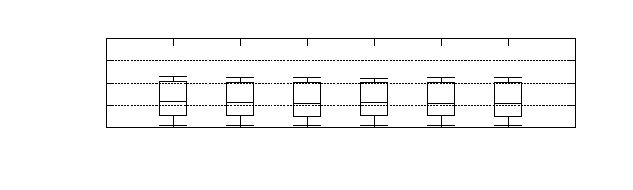
\includegraphics[width={280.00bp},height={75.60bp}]{images/boxPlot_risk}}}%
    \gplfronttext
  \end{picture}%
\endgroup
}
% REVISED FOR TMLR (erratum)
\caption{Empirical acceptance rate $\mathcal{C}$
across six expansion iterations on the 102 UCR datasets.
Median $\mathcal{C}$ stays in the $0.71$-$0.73$ band with
$Q_1 \approx 0.5$ and $Q_3 \approx 0.8$ across iterations, and shows
no systematic decline as $k$ grows: the rejection step retains the
majority of candidates at every step.}
\label{fig:risk-boxplot}
\end{figure}

The stability of the median across iterations is consistent with
Proposition~\ref{prop:variance}: the contrastive margin enforced
by $\mathcal{L}_{\text{cluster}}$ keeps $m/\sigma_w$ above
$2\sqrt{\alpha}$ across iterations, so the operating point stays in
the class-preserving regime of Figure~\ref{fig:prop1-heatmap}.
% REVISED FOR TMLR (erratum)
At $\alpha \approx 2.6$, this places the operating point
slightly above the bold curve $m/\sigma_w = 2\sqrt{\alpha} \approx
3.2$, in the region where the theoretical heatmap predicts
acceptance close to $0.7$, consistent with the empirical
$0.71$-$0.73$ band observed here.


% ========== Complexity & wall-clock (TMLR addition) ==========
% -----------------------------------------------------------------
% ADDED FOR TMLR (review-driven) — complexity + wall-clock analysis.
% Not present in the ICML version. Responds to ICML reviewers
% uqH7 W3 and siJn W3.
% Rebuttal source: Publication/ASCENSION/
%   ASCENSION_Response_Realism_Anisotropy.md (wall-clock table).
% -----------------------------------------------------------------

\section{Complexity}
\label{sec:complexity:big_o}

Let $N$ be the training-set size, $E$ the number of training
epochs, $D$ the input dimension (TS length), $H$ the
hidden width, $S$ the number of synthetic samples, and $T$ the
number of outer iterations. \tablename~\ref{tab:complexity} summarises
the asymptotic training and generation costs by method family.

\begin{table}[H]
\centering
\small
\caption{Asymptotic training and generation complexity by method
family. $T$ is the number of outer ASCENSION iterations or the
number of denoising steps for diffusion methods (typically
$T \approx 1000$).}
\label{tab:complexity}
\begin{tabular}{lll}
\toprule
\textbf{Method family} & \textbf{Training} & \textbf{Per-sample generation} \\
\midrule
FAA (transformation)     & n/a                                        & $\mathcal{O}(D)$ \\
VaDE / KoVAE             & $\mathcal{O}(N \cdot E \cdot D \cdot H)$   & $\mathcal{O}(D \cdot H)$ \\
TS-GAN / LatentAugment   & $\mathcal{O}(N \cdot E \cdot D \cdot H)$   & $\mathcal{O}(D \cdot H)$ \\
Diffusion-TS / ImagenTime& $\mathcal{O}(N \cdot E \cdot D \cdot H)$   & $\mathcal{O}(T \cdot D \cdot H)$ \\
\textbf{ASCENSION}       & $\mathcal{O}(T_{\text{outer}} \cdot N \cdot E \cdot D \cdot H)$ & $\mathcal{O}(D \cdot H)$ \\
\bottomrule
\end{tabular}
\end{table}

At the canonical setting $T_{\text{outer}} = 1$, ASCENSION's
training cost matches other VAE baselines. The crucial gap is at
generation time: ASCENSION produces each synthetic instance with
a single forward pass through the decoder, whereas diffusion
baselines require $\sim 1000$ sequential denoising steps.

\section{Wall-clock timing}
\label{sec:complexity:wallclock}

\tablename~\ref{tab:wallclock} reports end-to-end wall-clock time
(generative-model training plus sample generation; downstream
classifier training is excluded as it is identical for every
method) on three UCR datasets chosen to cover the dataset-size
range. ASCENSION is run with $\alpha = 2.6$, the mean of the
per-dataset best $\alpha$ values across our sweep
(Tables~\ref{Tab:app:bestconfig:resnet}--\ref{Tab:app:bestconfig:moment}).
All measurements on the same NVIDIA RTX 4080 Super used
for the main-results experiments.

\begin{table}[H]
\centering
\small
\caption{Wall-clock time (seconds) for generative-model training
plus generation, on three representative UCR datasets. Same
hardware and software stack as the main experiments.}
\label{tab:wallclock}
\begin{tabular}{@{}lrrrrrrr@{}}
\toprule
\textbf{Dataset} & FAA & VaDE & Time-DDPM & TTS-GAN &
\textbf{ASCENSION} & Diffusion-TS & ImagenTime \\
\midrule
Coffee  ($n\!=\!28$)   & $<\!0.1$ & 0.8 & 0.6 & 4.2  & \textbf{1.0}  & 13.2 & 20.3 \\
ECG200  ($n\!=\!100$)  & $<\!0.1$ & 1.9 & 2.2 & 8.7  & \textbf{2.8}  & 24.5 & 74.7 \\
FaceAll ($n\!=\!560$)  & $0.01$   & 5.8 & 5.7 & 25.8 & \textbf{11.0} & 89.1 & 188.9 \\
\bottomrule
\end{tabular}
\end{table}

ASCENSION is roughly an order of magnitude faster than
Diffusion-TS ($\sim 9$--$13\times$) and $15$--$27\times$ faster
than ImagenTime, both of which require hundreds of sequential
denoising steps per sample. It is $2$--$4\times$ faster than
TTS-GAN. It is in the same computational range as VaDE and
Time-DDPM, though consistently a bit slower because it
additionally computes the contrastive loss. FAA is near-instant
as it applies fixed transformations with no training but does
not offer downstream gain
(\tablename~\ref{tab:main-results}).



% ========== Detailed classification performance (ICML app:Exp:large:Classif) ==========
\section{Detailed classification performance} \label{app:per_dataset}
%\subsection{Detailed classification performance} \label{app:per_dataset}
This section analyses average classification accuracy changes across the 11 UCR domains (\tablename~\ref{tab:datasets_types}), with mean gains and drops reported in \tablename s~\ref{Tab:MeanImprov_ResNet}--\ref{Tab:MeanNegative_Moment} for ResNet, FCN, and Moment. \tablename s~\ref{Tab:Macro_ResNet}--\ref{Tab:Macro_Moment} aggregate these per-domain results into the five macro-domains defined in Appendix~\ref{app:domain-coverage}.
% ADDED FOR TMLR (rebuttal C4)
The per-dataset values reported in this section are single-run, and the cross-run variability of the ASCENSION gain under the fixed configuration is quantified in Appendix~\ref{app:per-dataset-std}.

%This section presents the analysis of the average classification accuracy changes across the 11 dataset domains defined in the UCR archive (see \tablename~\ref{tab:datasets_types}). \tablename s~\ref{Tab:MeanImprov_ResNet}-\ref{Tab:MeanNegative_ResNet} and \tablename s~\ref{Tab:MeanImprov_FCN}-\ref{Tab:MeanNegative_FCN} report the mean improvements and deteriorations (worsened) for ResNet and FCN, respectively.


% Flush any pending floats from the preceding section before entering landscape:
% without this, LaTeX can error "Float(s) lost" at \begin{landscape} when the
% main-body floats haven't placed yet (TMLR page area is narrower than ICML's
% article class, which is why ICML compiled fine without the clearpage).

\begin{landscape}
\begin{table}[h]
    \centering
    \caption{Mean improvement in classification accuracy across dataset domains (ResNet) best in bold.\label{Tab:MeanImprov_ResNet}}
    \scalebox{0.87}{
    \begin{tabular}{@{}lcccccccccccccccccc@{}}
    \toprule
    \textbf{Type} & \multicolumn{2}{c}{\textbf{ASCENSION}} & \multicolumn{2}{c}{\textbf{Diffusion-TS}} & \multicolumn{2}{c}{\textbf{FAA}} & \multicolumn{2}{c}{\textbf{ImagenTime}} & \multicolumn{2}{c}{\textbf{KoVAE}} & \multicolumn{2}{c}{\textbf{LA}} & \multicolumn{2}{c}{\textbf{Time-DDPM}} & \multicolumn{2}{c}{\textbf{TTS-GAN}} & \multicolumn{2}{c}{\textbf{VaDE}} \\
    \cmidrule(r){2-3} \cmidrule(r){4-5} \cmidrule(r){6-7} \cmidrule(r){8-9} \cmidrule(r){10-11} \cmidrule(r){12-13} \cmidrule(r){14-15} \cmidrule(r){16-17} \cmidrule(r){18-19}
    & $\uparrow$Nb & $\uparrow\overline{\Delta\mathrm{Acc}}$ & $\uparrow$Nb & $\uparrow\overline{\Delta\mathrm{Acc}}$ & $\uparrow$Nb & $\uparrow\overline{\Delta\mathrm{Acc}}$ & $\uparrow$Nb & $\uparrow\overline{\Delta\mathrm{Acc}}$ & $\uparrow$Nb & $\uparrow\overline{\Delta\mathrm{Acc}}$ & $\uparrow$Nb & $\uparrow\overline{\Delta\mathrm{Acc}}$ & $\uparrow$Nb & $\uparrow\overline{\Delta\mathrm{Acc}}$ & $\uparrow$Nb & $\uparrow\overline{\Delta\mathrm{Acc}}$ & $\uparrow$Nb & $\uparrow\overline{\Delta\mathrm{Acc}}$ \\
    \midrule
Device    & 3/8 & 1.4\% & 1/8 & 1.3\% & 4/8 & 4.4\% & 1/8 & 1.9\% & \textbf{5/8} & \textbf{1.0\%} & 1/8 & 8.9\% & 1/8 & 13.7\% & 2/8 & 0.3\% & 3/8 & 2.0\% \\
Image    & \textbf{22/30} & \textbf{3.7\%} & 8/30 & 1.5\% & 4/30 & 8.2\% & 5/30 & 1.8\% & 11/30 & 1.6\% & 3/30 & 4.0\% & 11/30 & 11.8\% & 10/30 & 2.5\% & 17/30 & 2.9\% \\
Simulated    & 1/8 & 0.6\% & \textbf{4/8} & \textbf{0.8\%} & 2/8 & 11.3\% & 1/8 & 0.6\% & 3/8 & 0.4\% & 2/8 & 1.3\% & 3/8 & 3.0\% & \textbf{4/8} & 0.8\% & 2/8 & 0.8\% \\
Spectro    & \textbf{5/8} & \textbf{16.4\%} & 1/8 & 0.4\% & 2/8 & 10.8\% & 2/8 & 1.6\% & 2/8 & 4.2\% & 1/8 & 3.3\% & 3/8 & 17.7\% & 3/8 & 2.6\% & 4/8 & 7.5\% \\
Sensor    & \textbf{12/19} & \textbf{2.8\%} & 4/19 & 0.6\% & 2/19 & 11.2\% & 3/19 & 0.3\% & 6/19 & 1.9\% & 5/19 & 2.5\% & 5/19 & 18.4\% & 4/19 & 3.9\% & 8/19 & 2.0\% \\
ECG    & \textbf{5/6} & \textbf{2.7\%} & 1/6 & 1.2\% & 1/6 & 13.8\% & 1/6 & 2.0\% & 2/6 & 0.7\% & 1/6 & 5.5\% & 2/6 & 7.7\% & 1/6 & 1.0\% & 2/6 & 2.9\% \\
EOG    & 0/2 & 0.0\% & 0/2 & 0.0\% & 0/2 & 0.0\% & 0/2 & 0.0\% & 1/2 & 4.4\% & 1/2 & 1.1\% & \textbf{2/2} & \textbf{35.7\%} & 0/2 & 0.0\% & 0/2 & 0.0\% \\
Motion    & \textbf{8/14} & \textbf{1.7\%} & 0/14 & 0.0\% & 1/14 & 2.2\% & 0/14 & 0.0\% & 5/14 & 0.5\% & 0/14 & 0.0\% & 7/14 & 17.0\% & 1/14 & 1.1\% & 5/14 & 1.4\% \\
EPG    & \textbf{0/2} & \textbf{0.0\%} & \textbf{0/2} & \textbf{0.0\%} & \textbf{0/2} & \textbf{0.0\%} & \textbf{0/2} & \textbf{0.0\%} & \textbf{0/2} & \textbf{0.0\%} & \textbf{0/2} & \textbf{0.0\%} & \textbf{0/2} & \textbf{0.0\%} & \textbf{0/2} & \textbf{0.0\%} & \textbf{0/2} & \textbf{0.0\%} \\
Power    & \textbf{1/1} & \textbf{2.2\%} & \textbf{1/1} & 2.1\% & 0/1 & 0.0\% & \textbf{1/1} & 1.1\% & \textbf{1/1} & 1.7\% & 0/1 & 0.0\% & 0/1 & 0.0\% & \textbf{1/1} & \textbf{2.2\%} & \textbf{1/1} & 1.7\% \\
Spectrum    & 2/4 & 4.4\% & 1/4 & 4.9\% & 3/4 & 5.1\% & 1/4 & 0.7\% & 2/4 & 2.6\% & 0/4 & 0.0\% & \textbf{4/4} & \textbf{29.1\%} & 0/4 & 0.0\% & 2/4 & 2.5\% \\
    \bottomrule
    \end{tabular}}

    \vspace{1cm}
    \caption{Mean worsened accuracy change across dataset domains (ResNet). Smallest reductions in bold.}\label{Tab:MeanNegative_ResNet}
    \scalebox{0.87}{
    \begin{tabular}{@{}lcccccccccccccccccc@{}}
    \toprule
    \textbf{Type} & \multicolumn{2}{c}{\textbf{ASCENSION}} & \multicolumn{2}{c}{\textbf{Diffusion-TS}} & \multicolumn{2}{c}{\textbf{FAA}} & \multicolumn{2}{c}{\textbf{ImagenTime}} & \multicolumn{2}{c}{\textbf{KoVAE}} & \multicolumn{2}{c}{\textbf{LA}} & \multicolumn{2}{c}{\textbf{Time-DDPM}} & \multicolumn{2}{c}{\textbf{TTS-GAN}} & \multicolumn{2}{c}{\textbf{VaDE}} \\
    \cmidrule(r){2-3} \cmidrule(r){4-5} \cmidrule(r){6-7} \cmidrule(r){8-9} \cmidrule(r){10-11} \cmidrule(r){12-13} \cmidrule(r){14-15} \cmidrule(r){16-17} \cmidrule(r){18-19}
    & $\downarrow$Nb & $\downarrow\overline{\Delta\mathrm{Acc}}$ & $\downarrow$Nb & $\downarrow\overline{\Delta\mathrm{Acc}}$ & $\downarrow$Nb & $\downarrow\overline{\Delta\mathrm{Acc}}$ & $\downarrow$Nb & $\downarrow\overline{\Delta\mathrm{Acc}}$ & $\downarrow$Nb & $\downarrow\overline{\Delta\mathrm{Acc}}$ & $\downarrow$Nb & $\downarrow\overline{\Delta\mathrm{Acc}}$ & $\downarrow$Nb & $\downarrow\overline{\Delta\mathrm{Acc}}$ & $\downarrow$Nb & $\downarrow\overline{\Delta\mathrm{Acc}}$ & $\downarrow$Nb & $\downarrow\overline{\Delta\mathrm{Acc}}$ \\
    \midrule
Device    & 5/8 & -2.1\% & 7/8 & -2.3\% & 4/8 & -5.7\% & 7/8 & -2.7\% & \textbf{1/8} & \textbf{-3.2\%} & 7/8 & -2.6\% & 7/8 & -15.5\% & 5/8 & -3.7\% & 5/8 & -2.2\% \\
Image    & \textbf{7/30} & \textbf{-1.5\%} & 22/30 & -11.9\% & 24/30 & -6.7\% & 21/30 & -7.3\% & 15/30 & -1.7\% & 24/30 & -4.4\% & 19/30 & -21.8\% & 18/30 & -6.1\% & 12/30 & -12.6\% \\
Simulated    & 4/8 & -0.5\% & 4/8 & -18.1\% & 6/8 & -6.7\% & 6/8 & -9.2\% & \textbf{2/8} & \textbf{-0.4\%} & 6/8 & -2.6\% & 5/8 & -28.8\% & 3/8 & -3.3\% & 6/8 & -9.4\% \\
Spectro    & \textbf{0/8} & \textbf{0.0\%} & 7/8 & -8.6\% & 6/8 & -20.6\% & 5/8 & -5.2\% & 5/8 & -5.3\% & 5/8 & -5.1\% & 5/8 & -23.3\% & 4/8 & -5.7\% & 3/8 & -1.6\% \\
Sensor    & \textbf{5/19} & \textbf{-0.7\%} & 13/19 & -7.3\% & 15/19 & -6.0\% & 13/19 & -4.6\% & 9/19 & -1.0\% & 11/19 & -2.8\% & 14/19 & -18.0\% & 12/19 & -6.1\% & 8/19 & -3.5\% \\
ECG    & \textbf{0/6} & \textbf{0.0\%} & 5/6 & -18.3\% & 4/6 & -25.3\% & 5/6 & -13.1\% & 4/6 & -2.2\% & 4/6 & -7.2\% & 4/6 & -36.0\% & 5/6 & -5.4\% & 4/6 & -16.6\% \\
EOG    & 2/2 & -7.3\% & 2/2 & -12.4\% & 2/2 & -15.1\% & 2/2 & -4.7\% & 1/2 & -2.8\% & 1/2 & -9.4\% & \textbf{0/2} & \textbf{0.0\%} & 2/2 & -27.8\% & 2/2 & -3.0\% \\
Motion    & \textbf{2/14} & \textbf{-1.6\%} & 13/14 & -5.3\% & 12/14 & -9.1\% & 12/14 & -3.9\% & 6/14 & -1.2\% & 13/14 & -4.2\% & 7/14 & -33.7\% & 12/14 & -15.6\% & 7/14 & -2.0\% \\
EPG    & \textbf{0/2} & \textbf{0.0\%} & \textbf{0/2} & \textbf{0.0\%} & \textbf{0/2} & \textbf{0.0\%} & \textbf{0/2} & \textbf{0.0\%} & \textbf{0/2} & \textbf{0.0\%} & \textbf{0/2} & \textbf{0.0\%} & 2/2 & -2.8\% & \textbf{0/2} & \textbf{0.0\%} & \textbf{0/2} & \textbf{0.0\%} \\
Power    & \textbf{0/1} & \textbf{0.0\%} & \textbf{0/1} & \textbf{0.0\%} & 1/1 & -2.2\% & \textbf{0/1} & \textbf{0.0\%} & \textbf{0/1} & \textbf{0.0\%} & 1/1 & -1.1\% & 1/1 & -8.5\% & \textbf{0/1} & \textbf{0.0\%} & \textbf{0/1} & \textbf{0.0\%} \\
Spectrum    & 2/4 & -2.9\% & 3/4 & -5.0\% & 1/4 & -6.0\% & 3/4 & -5.9\% & 2/4 & -6.1\% & 3/4 & -1.7\% & \textbf{0/4} & \textbf{0.0\%} & 4/4 & -8.3\% & 2/4 & -4.7\% \\
    \bottomrule
    \end{tabular}}
\end{table}
\end{landscape}
\clearpage
\begin{landscape}
\begin{table}[h]
    \centering
    \caption{Mean improvement in classification accuracy across dataset domains (FCN) best in bold.\label{Tab:MeanImprov_FCN}}
    \scalebox{0.87}{
    \begin{tabular}{@{}lcccccccccccccccccc@{}}
    \toprule
    \textbf{Type} & \multicolumn{2}{c}{\textbf{ASCENSION}} & \multicolumn{2}{c}{\textbf{Diffusion-TS}} & \multicolumn{2}{c}{\textbf{FAA}} & \multicolumn{2}{c}{\textbf{ImagenTime}} & \multicolumn{2}{c}{\textbf{KoVAE}} & \multicolumn{2}{c}{\textbf{LA}} & \multicolumn{2}{c}{\textbf{Time-DDPM}} & \multicolumn{2}{c}{\textbf{TTS-GAN}} & \multicolumn{2}{c}{\textbf{VaDE}} \\
    \cmidrule(r){2-3} \cmidrule(r){4-5} \cmidrule(r){6-7} \cmidrule(r){8-9} \cmidrule(r){10-11} \cmidrule(r){12-13} \cmidrule(r){14-15} \cmidrule(r){16-17} \cmidrule(r){18-19}
    & $\uparrow$Nb & $\uparrow\overline{\Delta\mathrm{Acc}}$ & $\uparrow$Nb & $\uparrow\overline{\Delta\mathrm{Acc}}$ & $\uparrow$Nb & $\uparrow\overline{\Delta\mathrm{Acc}}$ & $\uparrow$Nb & $\uparrow\overline{\Delta\mathrm{Acc}}$ & $\uparrow$Nb & $\uparrow\overline{\Delta\mathrm{Acc}}$ & $\uparrow$Nb & $\uparrow\overline{\Delta\mathrm{Acc}}$ & $\uparrow$Nb & $\uparrow\overline{\Delta\mathrm{Acc}}$ & $\uparrow$Nb & $\uparrow\overline{\Delta\mathrm{Acc}}$ & $\uparrow$Nb & $\uparrow\overline{\Delta\mathrm{Acc}}$ \\
    \midrule
Device    & 4/8 & 3.5\% & \textbf{5/8} & \textbf{3.2\%} & 1/8 & 7.2\% & 4/8 & 0.7\% & 4/8 & 0.9\% & 4/8 & 1.0\% & 4/8 & 20.2\% & 3/8 & 0.9\% & 4/8 & 2.7\% \\
Image    & \textbf{17/30} & \textbf{3.1\%} & 13/30 & 3.8\% & 2/30 & 7.3\% & 9/30 & 2.9\% & 12/30 & 2.3\% & 14/30 & 2.1\% & 13/30 & 17.0\% & 11/30 & 3.2\% & 15/30 & 3.5\% \\
Simulated    & \textbf{5/8} & \textbf{0.4\%} & 3/8 & 2.8\% & 3/8 & 3.6\% & 0/8 & 0.0\% & 3/8 & 0.6\% & 0/8 & 0.0\% & 1/8 & 12.6\% & 4/8 & 0.9\% & 0/8 & 0.0\% \\
Spectro    & \textbf{8/8} & \textbf{12.1\%} & 4/8 & 3.6\% & 2/8 & 11.3\% & 5/8 & 3.7\% & 2/8 & 6.8\% & 2/8 & 1.4\% & 4/8 & 8.3\% & 3/8 & 4.8\% & 3/8 & 3.7\% \\
Sensor    & 7/19 & 1.8\% & 7/19 & 2.4\% & 3/19 & 10.1\% & \textbf{9/19} & \textbf{2.4\%} & 6/19 & 1.2\% & 8/19 & 1.9\% & 4/19 & 19.9\% & 6/19 & 3.4\% & 7/19 & 2.1\% \\
ECG    & \textbf{5/6} & \textbf{3.5\%} & 1/6 & 4.7\% & 0/6 & 0.0\% & 2/6 & 5.5\% & 4/6 & 2.5\% & 4/6 & 3.7\% & 2/6 & 10.4\% & 4/6 & 4.8\% & 1/6 & 9.2\% \\
EOG    & \textbf{1/2} & 1.9\% & 0/2 & 0.0\% & 0/2 & 0.0\% & \textbf{1/2} & 1.1\% & 0/2 & 0.0\% & \textbf{1/2} & 1.1\% & \textbf{1/2} & \textbf{39.3\%} & 0/2 & 0.0\% & 0/2 & 0.0\% \\
Motion    & 7/14 & 2.1\% & 1/14 & 0.5\% & 2/14 & 3.3\% & 6/14 & 1.8\% & 6/14 & 1.3\% & \textbf{9/14} & 2.9\% & \textbf{9/14} & \textbf{13.6\%} & 3/14 & 1.7\% & \textbf{9/14} & 2.8\% \\
EPG    & \textbf{0/2} & \textbf{0.0\%} & \textbf{0/2} & \textbf{0.0\%} & \textbf{0/2} & \textbf{0.0\%} & \textbf{0/2} & \textbf{0.0\%} & \textbf{0/2} & \textbf{0.0\%} & \textbf{0/2} & \textbf{0.0\%} & \textbf{0/2} & \textbf{0.0\%} & \textbf{0/2} & \textbf{0.0\%} & \textbf{0/2} & \textbf{0.0\%} \\
Power    & 0/1 & 0.0\% & 0/1 & 0.0\% & 0/1 & 0.0\% & \textbf{1/1} & \textbf{1.7\%} & 0/1 & 0.0\% & \textbf{1/1} & 0.6\% & 0/1 & 0.0\% & \textbf{1/1} & \textbf{1.7\%} & \textbf{1/1} & 0.6\% \\
Spectrum    & 2/4 & 5.7\% & 2/4 & 5.5\% & 1/4 & 6.8\% & 1/4 & 9.3\% & \textbf{4/4} & 4.0\% & 1/4 & 7.5\% & \textbf{4/4} & \textbf{25.2\%} & 1/4 & 0.7\% & 2/4 & 8.9\% \\
    \bottomrule
    \end{tabular}}

    \vspace{1cm}
    \caption{Mean worsened accuracy change across dataset domains (FCN). Smallest reductions in bold.}\label{Tab:MeanNegative_FCN}
    \scalebox{0.86}{
    \begin{tabular}{@{}lcccccccccccccccccc@{}}
    \toprule
    \textbf{Type} & \multicolumn{2}{c}{\textbf{ASCENSION}} & \multicolumn{2}{c}{\textbf{Diffusion-TS}} & \multicolumn{2}{c}{\textbf{FAA}} & \multicolumn{2}{c}{\textbf{ImagenTime}} & \multicolumn{2}{c}{\textbf{KoVAE}} & \multicolumn{2}{c}{\textbf{LA}} & \multicolumn{2}{c}{\textbf{Time-DDPM}} & \multicolumn{2}{c}{\textbf{TTS-GAN}} & \multicolumn{2}{c}{\textbf{VaDE}} \\
    \cmidrule(r){2-3} \cmidrule(r){4-5} \cmidrule(r){6-7} \cmidrule(r){8-9} \cmidrule(r){10-11} \cmidrule(r){12-13} \cmidrule(r){14-15} \cmidrule(r){16-17} \cmidrule(r){18-19}
    & $\downarrow$Nb & $\downarrow\overline{\Delta\mathrm{Acc}}$ & $\downarrow$Nb & $\downarrow\overline{\Delta\mathrm{Acc}}$ & $\downarrow$Nb & $\downarrow\overline{\Delta\mathrm{Acc}}$ & $\downarrow$Nb & $\downarrow\overline{\Delta\mathrm{Acc}}$ & $\downarrow$Nb & $\downarrow\overline{\Delta\mathrm{Acc}}$ & $\downarrow$Nb & $\downarrow\overline{\Delta\mathrm{Acc}}$ & $\downarrow$Nb & $\downarrow\overline{\Delta\mathrm{Acc}}$ & $\downarrow$Nb & $\downarrow\overline{\Delta\mathrm{Acc}}$ & $\downarrow$Nb & $\downarrow\overline{\Delta\mathrm{Acc}}$ \\
    \midrule
Device    & 4/8 & -2.2\% & \textbf{3/8} & -5.8\% & 7/8 & -9.0\% & 4/8 & -4.2\% & 4/8 & -3.7\% & 4/8 & -3.2\% & 4/8 & -27.9\% & \textbf{3/8} & -3.8\% & \textbf{3/8} & \textbf{-3.0\%} \\
Image    & \textbf{12/30} & -3.1\% & 17/30 & -22.6\% & 28/30 & -15.9\% & 20/30 & -3.0\% & 16/30 & -1.7\% & \textbf{12/30} & \textbf{-2.0\%} & 17/30 & -20.0\% & 17/30 & -5.1\% & 13/30 & -10.2\% \\
Simulated    & \textbf{1/8} & \textbf{-1.4\%} & 3/8 & -20.3\% & 5/8 & -18.2\% & 6/8 & -1.6\% & 5/8 & -1.0\% & 4/8 & -2.8\% & 6/8 & -20.2\% & 2/8 & -5.8\% & 6/8 & -10.4\% \\
Spectro    & \textbf{0/8} & \textbf{0.0\%} & 4/8 & -11.7\% & 6/8 & -30.4\% & 2/8 & -6.1\% & 4/8 & -4.3\% & 4/8 & -4.9\% & 4/8 & -24.5\% & 3/8 & -3.2\% & 3/8 & -2.7\% \\
Sensor    & 9/19 & -1.6\% & 10/19 & -8.4\% & 16/19 & -10.5\% & \textbf{7/19} & -2.2\% & \textbf{7/19} & \textbf{-1.1\%} & 8/19 & -1.7\% & 15/19 & -25.0\% & 9/19 & -5.4\% & 9/19 & -2.3\% \\
ECG    & \textbf{1/6} & \textbf{-2.0\%} & 5/6 & -19.7\% & 6/6 & -22.0\% & 4/6 & -2.3\% & 2/6 & -9.5\% & 2/6 & -2.6\% & 4/6 & -13.1\% & 2/6 & -7.3\% & 4/6 & -12.3\% \\
EOG    & 1/2 & -1.1\% & 2/2 & -8.6\% & 2/2 & -16.0\% & 1/2 & -0.6\% & 2/2 & -1.0\% & \textbf{0/2} & \textbf{0.0\%} & 1/2 & -11.3\% & 2/2 & -27.1\% & 2/2 & -6.2\% \\
Motion    & 5/14 & -3.8\% & 12/14 & -6.4\% & 11/14 & -12.7\% & 7/14 & -3.1\% & 5/14 & -1.0\% & \textbf{3/14} & \textbf{-1.8\%} & 5/14 & -26.4\% & 8/14 & -14.5\% & \textbf{3/14} & -3.9\% \\
EPG    & \textbf{0/2} & \textbf{0.0\%} & \textbf{0/2} & \textbf{0.0\%} & \textbf{0/2} & \textbf{0.0\%} & \textbf{0/2} & \textbf{0.0\%} & \textbf{0/2} & \textbf{0.0\%} & \textbf{0/2} & \textbf{0.0\%} & 2/2 & -11.1\% & \textbf{0/2} & \textbf{0.0\%} & \textbf{0/2} & \textbf{0.0\%} \\
Power    & \textbf{0/1} & \textbf{0.0\%} & 1/1 & -1.1\% & 1/1 & -3.9\% & \textbf{0/1} & \textbf{0.0\%} & 1/1 & -0.6\% & \textbf{0/1} & \textbf{0.0\%} & 1/1 & -89.6\% & \textbf{0/1} & \textbf{0.0\%} & \textbf{0/1} & \textbf{0.0\%} \\
Spectrum    & 1/4 & -2.0\% & 2/4 & -4.2\% & 3/4 & -6.1\% & 2/4 & -4.2\% & \textbf{0/4} & \textbf{0.0\%} & 2/4 & -5.0\% & \textbf{0/4} & \textbf{0.0\%} & 3/4 & -15.9\% & 2/4 & -4.7\% \\
    \bottomrule
    \end{tabular}}
\end{table}
\end{landscape}
\clearpage
\begin{landscape}
\begin{table}[h]
    \centering
    \caption{Mean improvement in classification accuracy across dataset domains (Moment) best in bold.\label{Tab:MeanImprov_Moment}}
    \scalebox{0.87}{
    \begin{tabular}{@{}lcccccccccccccccccc@{}}
    \toprule
    \textbf{Type} & \multicolumn{2}{c}{\textbf{ASCENSION}} & \multicolumn{2}{c}{\textbf{Diffusion-TS}} & \multicolumn{2}{c}{\textbf{FAA}} & \multicolumn{2}{c}{\textbf{ImagenTime}} & \multicolumn{2}{c}{\textbf{KoVAE}} & \multicolumn{2}{c}{\textbf{LA}} & \multicolumn{2}{c}{\textbf{Time-DDPM}} & \multicolumn{2}{c}{\textbf{TTS-GAN}} & \multicolumn{2}{c}{\textbf{VaDE}} \\
    \cmidrule(r){2-3} \cmidrule(r){4-5} \cmidrule(r){6-7} \cmidrule(r){8-9} \cmidrule(r){10-11} \cmidrule(r){12-13} \cmidrule(r){14-15} \cmidrule(r){16-17} \cmidrule(r){18-19}
    & $\uparrow$Nb & $\uparrow\overline{\Delta\mathrm{Acc}}$ & $\uparrow$Nb & $\uparrow\overline{\Delta\mathrm{Acc}}$ & $\uparrow$Nb & $\uparrow\overline{\Delta\mathrm{Acc}}$ & $\uparrow$Nb & $\uparrow\overline{\Delta\mathrm{Acc}}$ & $\uparrow$Nb & $\uparrow\overline{\Delta\mathrm{Acc}}$ & $\uparrow$Nb & $\uparrow\overline{\Delta\mathrm{Acc}}$ & $\uparrow$Nb & $\uparrow\overline{\Delta\mathrm{Acc}}$ & $\uparrow$Nb & $\uparrow\overline{\Delta\mathrm{Acc}}$ & $\uparrow$Nb & $\uparrow\overline{\Delta\mathrm{Acc}}$ \\
    \midrule
Device    & \textbf{6/8} & \textbf{2.1\%} & 3/8 & 1.5\% & 5/8 & 15.1\% & 1/8 & 0.1\% & 1/8 & 2.4\% & 2/8 & 0.7\% & 2/8 & 0.9\% & 2/8 & 0.5\% & 1/8 & 0.5\% \\
Image    & \textbf{24/30} & \textbf{3.5\%} & 11/30 & 4.5\% & 16/30 & 5.8\% & 9/30 & 2.8\% & 9/30 & 4.8\% & 10/30 & 3.6\% & 12/30 & 3.8\% & 14/30 & 3.9\% & 12/30 & 3.8\% \\
Simulated    & \textbf{4/8} & 4.0\% & 1/8 & 2.3\% & \textbf{4/8} & \textbf{9.8\%} & 2/8 & 0.8\% & 1/8 & 2.7\% & 2/8 & 4.5\% & 3/8 & 4.1\% & 3/8 & 3.3\% & \textbf{4/8} & 3.1\% \\
Spectro    & \textbf{5/8} & \textbf{5.0\%} & 1/8 & 1.1\% & 4/8 & 7.1\% & 0/8 & 0.0\% & 0/8 & 0.0\% & 0/8 & 0.0\% & 0/8 & 0.0\% & 1/8 & 3.6\% & 0/8 & 0.0\% \\
Sensor    & \textbf{13/19} & \textbf{6.1\%} & 5/19 & 2.7\% & 9/19 & 9.1\% & 6/19 & 2.2\% & 10/19 & 3.8\% & 9/19 & 2.3\% & 8/19 & 5.4\% & 11/19 & 4.0\% & 9/19 & 2.6\% \\
ECG    & \textbf{4/6} & 2.7\% & 1/6 & 0.4\% & 3/6 & 7.6\% & 2/6 & 3.3\% & 2/6 & 0.9\% & 2/6 & 0.7\% & \textbf{4/6} & 1.4\% & \textbf{4/6} & \textbf{2.9\%} & 2/6 & 2.1\% \\
EOG    & \textbf{1/2} & \textbf{3.0\%} & 0/2 & 0.0\% & 0/2 & 0.0\% & 0/2 & 0.0\% & 0/2 & 0.0\% & 0/2 & 0.0\% & 0/2 & 0.0\% & 0/2 & 0.0\% & 0/2 & 0.0\% \\
Motion    & \textbf{11/14} & \textbf{2.4\%} & 4/14 & 3.1\% & 5/14 & 4.6\% & 3/14 & 0.8\% & 3/14 & 3.8\% & 4/14 & 2.1\% & 4/14 & 2.6\% & 5/14 & 2.8\% & 6/14 & 2.5\% \\
EPG    & 1/2 & 5.2\% & 1/2 & 1.2\% & \textbf{2/2} & \textbf{7.6\%} & 1/2 & 1.2\% & 0/2 & 0.0\% & 0/2 & 0.0\% & 1/2 & 2.4\% & 0/2 & 0.0\% & 0/2 & 0.0\% \\
Power    & \textbf{0/1} & \textbf{0.0\%} & \textbf{0/1} & \textbf{0.0\%} & \textbf{0/1} & \textbf{0.0\%} & \textbf{0/1} & \textbf{0.0\%} & \textbf{0/1} & \textbf{0.0\%} & \textbf{0/1} & \textbf{0.0\%} & \textbf{0/1} & \textbf{0.0\%} & \textbf{0/1} & \textbf{0.0\%} & \textbf{0/1} & \textbf{0.0\%} \\
Spectrum    & \textbf{3/4} & \textbf{4.4\%} & 1/4 & 4.0\% & 2/4 & 5.4\% & 1/4 & 2.8\% & 1/4 & 0.8\% & 2/4 & 2.1\% & 1/4 & 12.0\% & 1/4 & 0.3\% & 1/4 & 2.0\% \\
    \bottomrule
    \end{tabular}}

    \vspace{1cm}
    \caption{Mean worsened accuracy change across dataset domains (Moment). Smallest reductions in bold.}\label{Tab:MeanNegative_Moment}
    \scalebox{0.87}{
    \begin{tabular}{@{}lcccccccccccccccccc@{}}
    \toprule
    \textbf{Type} & \multicolumn{2}{c}{\textbf{ASCENSION}} & \multicolumn{2}{c}{\textbf{Diffusion-TS}} & \multicolumn{2}{c}{\textbf{FAA}} & \multicolumn{2}{c}{\textbf{ImagenTime}} & \multicolumn{2}{c}{\textbf{KoVAE}} & \multicolumn{2}{c}{\textbf{LA}} & \multicolumn{2}{c}{\textbf{Time-DDPM}} & \multicolumn{2}{c}{\textbf{TTS-GAN}} & \multicolumn{2}{c}{\textbf{VaDE}} \\
    \cmidrule(r){2-3} \cmidrule(r){4-5} \cmidrule(r){6-7} \cmidrule(r){8-9} \cmidrule(r){10-11} \cmidrule(r){12-13} \cmidrule(r){14-15} \cmidrule(r){16-17} \cmidrule(r){18-19}
    & $\downarrow$Nb & $\downarrow\overline{\Delta\mathrm{Acc}}$ & $\downarrow$Nb & $\downarrow\overline{\Delta\mathrm{Acc}}$ & $\downarrow$Nb & $\downarrow\overline{\Delta\mathrm{Acc}}$ & $\downarrow$Nb & $\downarrow\overline{\Delta\mathrm{Acc}}$ & $\downarrow$Nb & $\downarrow\overline{\Delta\mathrm{Acc}}$ & $\downarrow$Nb & $\downarrow\overline{\Delta\mathrm{Acc}}$ & $\downarrow$Nb & $\downarrow\overline{\Delta\mathrm{Acc}}$ & $\downarrow$Nb & $\downarrow\overline{\Delta\mathrm{Acc}}$ & $\downarrow$Nb & $\downarrow\overline{\Delta\mathrm{Acc}}$ \\
    \midrule
Device    & \textbf{1/8} & \textbf{-0.5\%} & 5/8 & -1.6\% & 3/8 & -4.5\% & 7/8 & -2.4\% & 7/8 & -3.4\% & 5/8 & -2.3\% & 6/8 & -1.9\% & 5/8 & -2.5\% & 6/8 & -1.7\% \\
Image    & \textbf{5/30} & \textbf{-1.1\%} & 18/30 & -11.7\% & 12/30 & -9.8\% & 19/30 & -6.0\% & 21/30 & -10.9\% & 20/30 & -4.9\% & 17/30 & -5.6\% & 16/30 & -4.2\% & 17/30 & -3.7\% \\
Simulated    & \textbf{2/8} & \textbf{-0.8\%} & 6/8 & -15.3\% & 4/8 & -12.4\% & 5/8 & -9.8\% & 6/8 & -12.6\% & 6/8 & -9.4\% & 5/8 & -8.5\% & 4/8 & -12.4\% & 4/8 & -9.9\% \\
Spectro    & \textbf{2/8} & \textbf{-7.2\%} & 6/8 & -15.4\% & 4/8 & -24.2\% & 7/8 & -13.8\% & 7/8 & -9.5\% & 6/8 & -10.2\% & 7/8 & -8.1\% & 6/8 & -8.7\% & 6/8 & -5.9\% \\
Sensor    & \textbf{4/19} & \textbf{-0.8\%} & 13/19 & -6.9\% & 7/19 & -9.7\% & 12/19 & -5.5\% & 7/19 & -5.0\% & 9/19 & -4.1\% & 9/19 & -5.4\% & 8/19 & -3.3\% & 9/19 & -4.0\% \\
ECG    & \textbf{1/6} & \textbf{-0.1\%} & 5/6 & -7.8\% & 3/6 & -4.2\% & 4/6 & -4.6\% & 4/6 & -31.2\% & 4/6 & -4.2\% & 2/6 & -59.1\% & \textbf{1/6} & -1.6\% & 4/6 & -20.9\% \\
EOG    & \textbf{1/2} & \textbf{-1.1\%} & 2/2 & -10.2\% & 2/2 & -12.6\% & 2/2 & -9.0\% & 2/2 & -9.4\% & 2/2 & -10.4\% & 2/2 & -7.3\% & 2/2 & -8.8\% & 2/2 & -7.5\% \\
Motion    & \textbf{2/14} & \textbf{-0.9\%} & 9/14 & -3.8\% & 8/14 & -15.9\% & 10/14 & -4.2\% & 10/14 & -25.2\% & 8/14 & -5.2\% & 9/14 & -2.6\% & 7/14 & -4.1\% & 5/14 & -3.8\% \\
EPG    & \textbf{0/2} & \textbf{0.0\%} & 1/2 & -4.8\% & \textbf{0/2} & \textbf{0.0\%} & 1/2 & -15.3\% & 2/2 & -5.2\% & 2/2 & -3.8\% & 1/2 & -12.4\% & 1/2 & -3.6\% & 2/2 & -8.4\% \\
Power    & \textbf{1/1} & \textbf{-2.8\%} & \textbf{1/1} & -3.3\% & \textbf{1/1} & -4.4\% & \textbf{1/1} & \textbf{-2.8\%} & \textbf{1/1} & -4.4\% & \textbf{1/1} & -3.9\% & \textbf{1/1} & -4.4\% & \textbf{1/1} & -6.1\% & \textbf{1/1} & -6.1\% \\
Spectrum    & \textbf{1/4} & \textbf{-0.2\%} & 3/4 & -3.9\% & 2/4 & -14.9\% & 2/4 & -1.6\% & 3/4 & -5.0\% & 2/4 & -1.7\% & 3/4 & -1.6\% & 3/4 & -4.1\% & 3/4 & -1.1\% \\
    \bottomrule
    \end{tabular}}
\end{table}
\end{landscape}
\clearpage
\begin{landscape}
\begin{table}[h]
    \centering
    \caption{Macro-domain breakdown -- ResNet: number of improved datasets ($\uparrow$Nb) out of total per macro-domain, and net mean accuracy change ($\overline{\Delta\mathrm{Acc}}$). Macro-domains group the 11 UCR raw types as follows: Industrial = Sensor + Device + Simulated + Power; Spectral = Spectro + Spectrum; Biomedical = ECG + EPG + EOG; Image and Motion are unchanged.}\label{Tab:Macro_ResNet}
    \scalebox{0.93}{
    \begin{tabular}{@{}lcccccccccccccccccc@{}}
    \toprule
    \textbf{Macro} & \multicolumn{2}{c}{\textbf{ASCENSION}} & \multicolumn{2}{c}{\textbf{Diffusion-TS}} & \multicolumn{2}{c}{\textbf{FAA}} & \multicolumn{2}{c}{\textbf{ImagenTime}} & \multicolumn{2}{c}{\textbf{KoVAE}} & \multicolumn{2}{c}{\textbf{LA}} & \multicolumn{2}{c}{\textbf{Time-DDPM}} & \multicolumn{2}{c}{\textbf{TTS-GAN}} & \multicolumn{2}{c}{\textbf{VaDE}} \\
    \cmidrule(r){2-3} \cmidrule(r){4-5} \cmidrule(r){6-7} \cmidrule(r){8-9} \cmidrule(r){10-11} \cmidrule(r){12-13} \cmidrule(r){14-15} \cmidrule(r){16-17} \cmidrule(r){18-19}
    & $\uparrow$Nb & $\overline{\Delta\mathrm{Acc}}$ & $\uparrow$Nb & $\overline{\Delta\mathrm{Acc}}$ & $\uparrow$Nb & $\overline{\Delta\mathrm{Acc}}$ & $\uparrow$Nb & $\overline{\Delta\mathrm{Acc}}$ & $\uparrow$Nb & $\overline{\Delta\mathrm{Acc}}$ & $\uparrow$Nb & $\overline{\Delta\mathrm{Acc}}$ & $\uparrow$Nb & $\overline{\Delta\mathrm{Acc}}$ & $\uparrow$Nb & $\overline{\Delta\mathrm{Acc}}$ & $\uparrow$Nb & $\overline{\Delta\mathrm{Acc}}$ \\
    \midrule
Industrial    & 17/36 & 0.7\% & 10/36 & -4.8\% & 8/36 & -2.6\% & 6/36 & -3.6\% & 15/36 & 0.2\% & 8/36 & -1.2\% & 9/36 & -11.1\% & 11/36 & -2.2\% & 14/36 & -1.9\% \\
Image    & 22/30 & 2.4\% & 8/30 & -8.3\% & 4/30 & -4.3\% & 5/30 & -4.8\% & 11/30 & -0.3\% & 3/30 & -3.1\% & 11/30 & -9.5\% & 10/30 & -2.8\% & 17/30 & -3.4\% \\
Motion    & 8/14 & 0.8\% & 0/14 & -4.9\% & 1/14 & -7.6\% & 0/14 & -3.3\% & 5/14 & -0.3\% & 0/14 & -3.9\% & 7/14 & -8.3\% & 1/14 & -13.3\% & 5/14 & -0.5\% \\
Spectral    & 7/12 & 7.1\% & 2/12 & -5.8\% & 5/12 & -7.7\% & 3/12 & -3.3\% & 4/12 & -2.1\% & 1/12 & -2.3\% & 7/12 & 4.4\% & 3/12 & -4.0\% & 6/12 & 1.7\% \\
Biomedical    & 5/10 & -0.1\% & 1/10 & -11.5\% & 1/10 & -11.7\% & 1/10 & -7.3\% & 3/10 & -0.6\% & 2/10 & -3.2\% & 4/10 & -6.3\% & 1/10 & -8.2\% & 2/10 & -6.7\% \\
    \bottomrule
    \end{tabular}}

    \vspace{1cm}

    \caption{Macro-domain breakdown -- FCN: number of improved datasets ($\uparrow$Nb) out of total per macro-domain, and net mean accuracy change ($\overline{\Delta\mathrm{Acc}}$). Macro-domains group the 11 UCR raw types as follows: Industrial = Sensor + Device + Simulated + Power; Spectral = Spectro + Spectrum; Biomedical = ECG + EPG + EOG; Image and Motion are unchanged.}\label{Tab:Macro_FCN}
    \scalebox{0.93}{
    \begin{tabular}{@{}lcccccccccccccccccc@{}}
    \toprule
    \textbf{Macro} & \multicolumn{2}{c}{\textbf{ASCENSION}} & \multicolumn{2}{c}{\textbf{Diffusion-TS}} & \multicolumn{2}{c}{\textbf{FAA}} & \multicolumn{2}{c}{\textbf{ImagenTime}} & \multicolumn{2}{c}{\textbf{KoVAE}} & \multicolumn{2}{c}{\textbf{LA}} & \multicolumn{2}{c}{\textbf{Time-DDPM}} & \multicolumn{2}{c}{\textbf{TTS-GAN}} & \multicolumn{2}{c}{\textbf{VaDE}} \\
    \cmidrule(r){2-3} \cmidrule(r){4-5} \cmidrule(r){6-7} \cmidrule(r){8-9} \cmidrule(r){10-11} \cmidrule(r){12-13} \cmidrule(r){14-15} \cmidrule(r){16-17} \cmidrule(r){18-19}
    & $\uparrow$Nb & $\overline{\Delta\mathrm{Acc}}$ & $\uparrow$Nb & $\overline{\Delta\mathrm{Acc}}$ & $\uparrow$Nb & $\overline{\Delta\mathrm{Acc}}$ & $\uparrow$Nb & $\overline{\Delta\mathrm{Acc}}$ & $\uparrow$Nb & $\overline{\Delta\mathrm{Acc}}$ & $\uparrow$Nb & $\overline{\Delta\mathrm{Acc}}$ & $\uparrow$Nb & $\overline{\Delta\mathrm{Acc}}$ & $\uparrow$Nb & $\overline{\Delta\mathrm{Acc}}$ & $\uparrow$Nb & $\overline{\Delta\mathrm{Acc}}$ \\
    \midrule
Industrial    & 16/36 & 0.1\% & 15/36 & -3.4\% & 7/36 & -7.7\% & 14/36 & -0.4\% & 13/36 & -0.4\% & 13/36 & -0.5\% & 9/36 & -14.6\% & 14/36 & -1.2\% & 12/36 & -1.9\% \\
Image    & 17/30 & 0.5\% & 13/30 & -11.2\% & 2/30 & -14.3\% & 9/30 & -1.2\% & 12/30 & 0.0\% & 14/30 & 0.2\% & 13/30 & -4.0\% & 11/30 & -1.7\% & 15/30 & -2.7\% \\
Motion    & 7/14 & -0.3\% & 1/14 & -5.5\% & 2/14 & -9.5\% & 6/14 & -0.8\% & 6/14 & 0.2\% & 9/14 & 1.5\% & 9/14 & -0.7\% & 3/14 & -7.9\% & 9/14 & 1.0\% \\
Spectral    & 10/12 & 8.9\% & 6/12 & -2.5\% & 3/12 & -14.3\% & 6/12 & 0.6\% & 6/12 & 1.0\% & 3/12 & -1.6\% & 8/12 & 3.0\% & 4/12 & -3.5\% & 5/12 & 1.0\% \\
Biomedical    & 6/10 & 1.6\% & 1/10 & -11.1\% & 0/10 & -16.4\% & 3/10 & 0.2\% & 4/10 & -1.1\% & 5/10 & 1.1\% & 3/10 & -2.6\% & 4/10 & -4.9\% & 1/10 & -5.2\% \\
    \bottomrule
    \end{tabular}}

    \vspace{1cm}

    \caption{Macro-domain breakdown -- Moment: number of improved datasets ($\uparrow$Nb) out of total per macro-domain, and net mean accuracy change ($\overline{\Delta\mathrm{Acc}}$). Macro-domains group the 11 UCR raw types as follows: Industrial = Sensor + Device + Simulated + Power; Spectral = Spectro + Spectrum; Biomedical = ECG + EPG + EOG; Image and Motion are unchanged.}\label{Tab:Macro_Moment}
    \scalebox{0.93}{
    \begin{tabular}{@{}lcccccccccccccccccc@{}}
    \toprule
    \textbf{Macro} & \multicolumn{2}{c}{\textbf{ASCENSION}} & \multicolumn{2}{c}{\textbf{Diffusion-TS}} & \multicolumn{2}{c}{\textbf{FAA}} & \multicolumn{2}{c}{\textbf{ImagenTime}} & \multicolumn{2}{c}{\textbf{KoVAE}} & \multicolumn{2}{c}{\textbf{LA}} & \multicolumn{2}{c}{\textbf{Time-DDPM}} & \multicolumn{2}{c}{\textbf{TTS-GAN}} & \multicolumn{2}{c}{\textbf{VaDE}} \\
    \cmidrule(r){2-3} \cmidrule(r){4-5} \cmidrule(r){6-7} \cmidrule(r){8-9} \cmidrule(r){10-11} \cmidrule(r){12-13} \cmidrule(r){14-15} \cmidrule(r){16-17} \cmidrule(r){18-19}
    & $\uparrow$Nb & $\overline{\Delta\mathrm{Acc}}$ & $\uparrow$Nb & $\overline{\Delta\mathrm{Acc}}$ & $\uparrow$Nb & $\overline{\Delta\mathrm{Acc}}$ & $\uparrow$Nb & $\overline{\Delta\mathrm{Acc}}$ & $\uparrow$Nb & $\overline{\Delta\mathrm{Acc}}$ & $\uparrow$Nb & $\overline{\Delta\mathrm{Acc}}$ & $\uparrow$Nb & $\overline{\Delta\mathrm{Acc}}$ & $\uparrow$Nb & $\overline{\Delta\mathrm{Acc}}$ & $\uparrow$Nb & $\overline{\Delta\mathrm{Acc}}$ \\
    \midrule
Industrial    & 23/36 & 2.8\% & 9/36 & -4.8\% & 18/36 & 1.7\% & 9/36 & -3.3\% & 12/36 & -2.7\% & 13/36 & -2.1\% & 13/36 & -1.4\% & 16/36 & -1.1\% & 14/36 & -1.6\% \\
Image    & 24/30 & 2.6\% & 11/30 & -5.4\% & 16/30 & -0.8\% & 9/30 & -3.0\% & 9/30 & -6.2\% & 10/30 & -2.0\% & 12/30 & -1.6\% & 14/30 & -0.4\% & 12/30 & -0.6\% \\
Motion    & 11/14 & 1.8\% & 4/14 & -1.6\% & 5/14 & -7.4\% & 3/14 & -2.8\% & 3/14 & -17.2\% & 4/14 & -2.4\% & 4/14 & -0.9\% & 5/14 & -1.1\% & 6/14 & -0.3\% \\
Spectral    & 8/12 & 2.0\% & 2/12 & -8.3\% & 6/12 & -7.3\% & 1/12 & -8.1\% & 1/12 & -6.8\% & 2/12 & -5.0\% & 1/12 & -4.1\% & 2/12 & -5.1\% & 1/12 & -3.1\% \\
Biomedical    & 6/10 & 1.8\% & 2/10 & -6.3\% & 5/10 & 0.0\% & 3/10 & -4.4\% & 2/10 & -15.2\% & 2/10 & -4.4\% & 5/10 & -13.7\% & 4/10 & -1.1\% & 2/10 & -11.1\% \\
    \bottomrule
    \end{tabular}}
\end{table}
\end{landscape}



% Hyperparameter Sensitivity Analysis
%\input{sections/appendix/hyperparameter_sensibility_analysis}


\begin{table*}[t]
    \centering  
    \caption{UCR dataset domains and their selected representative datasets}\label{tab:datasets_types}
    \footnotesize
    \scalebox{1}{
    \begin{tabular}{lll}
        \toprule
        \textbf{Type} & \textbf{Representative dataset} & \textbf{Description} \\
        \midrule
        Device       & ACSF1          & Measurements of alternating current signals for predictive maintenance  \\
        Image        & BeetleFly       & Shape-based image classification of beetle and fly outlines \\
        Simulated    & UMD       & Simulated control processes data\\
        Spectro      & Ham       & Spectroscopy data to identify types of ham based on chemical properties \\
        Sensor       & Car        & Sensor readings collected from a car, used for detecting driving conditions \\
        ECG          & ECG200          & Electrocardiogram (ECG) readings used to detect heart abnormalities \\
        EOG          & EOGVerticalSignal  & Electrooculography (EOG) signals capturing eye movement patterns \\
        Motion       & Worms       & Motion sensor data capturing worm movements for classification  \\
        EPG & InsectEPGRegularTrain & Electrical penetration graph (EPG) signals capturing insect feeding behaviour \\
        
        
        Power & PowerCons & Power consumption measurements for energy usage\\
        
        
        
        Spectrum     & SemgHandMovementCh2   & Electromyography (EMG) data of hand movements, recorded across channels \\
        \bottomrule
    \end{tabular}
    }
\end{table*}
% REVISED FOR TMLR (rebuttal C1)
\tablename s~\ref{Tab:app:bestconfig:resnet}, \ref{Tab:app:bestconfig:fcn}, and~\ref{Tab:app:bestconfig:moment} report the best $(\text{iter.}, \alpha)$ configuration per dataset for each of the three classifiers used in \tablename~\ref{tab:best-config}, together with the corresponding accuracy improvement ($\overline{\Delta\mathrm{Acc}} = \mathrm{aug\_acc} - \mathrm{base\_acc}$).

\paragraph{Augmentation budget.}
% REVISED FOR TMLR (erratum, one-to-one budget)
All methods use the same per-class generation budget, which follows the empirical class distribution: at each outer iteration, $|\mathcal{I}_y|$ candidate samples are drawn per class $y$, one per real sample, $n$ in total. Baselines add all $n$ candidates to the training set. For ASCENSION, the Bayes-region rejection step (Definition~\ref{def:bayes-region}) discards out-of-region candidates, so the realised number of synthetic samples that ASCENSION adds to the training set is in practice smaller than this budget and varies across datasets (median acceptance rate $\approx 0.71$-$0.73$, see Appendix~\ref{app:acceptance}).

\begin{table}[H]
\centering
% REVISED FOR TMLR (rebuttal C1)
\caption{Best $(\text{iter.}, \alpha)$ configuration per dataset for the ResNet classifier in \tablename~\ref{tab:best-config}, with the corresponding accuracy improvement ($\overline{\Delta\mathrm{Acc}} = \mathrm{augmentation\_accuracy} - \mathrm{base\_accuracy}$).}\label{Tab:app:bestconfig:resnet}
\setlength{\tabcolsep}{3pt}
\resizebox{\textwidth}{!}{%
\begin{tabular}{lr | lr || lr | lr}
\toprule
\# & Dataset & (iter., $\alpha$) & $\overline{\Delta\mathrm{Acc}}$ & \# & Dataset & (iter., $\alpha$) & $\overline{\Delta\mathrm{Acc}}$ \\
\midrule
D1 & ACSF1 & (2, 3.2) & 0.03 & D52 & Meat & (1, 1.5) & -0.00 \\
D2 & Adiac & (1, 2) & 0.02 & D53 & MedicalImages & (1, 4.2) & 0.02 \\
D3 & ArrowHead & (3, 4.7) & 0.02 & D54 & MiddlePhalanxOutlineAgeGroup & (2, 4.9) & 0.01 \\
D4 & BME & (3, 1.2) & -0.01 & D55 & MiddlePhalanxOutlineCorrect & (1, 3.7) & -0.01 \\
D5 & Beef & (1, 1.3) & 0.20 & D56 & MiddlePhalanxTW & (1, 4) & 0.01 \\
D6 & BeetleFly & (1, 1.2) & 0.00 & D57 & MixedShapesRegularTrain & (1, 1.3) & 0.01 \\
D7 & BirdChicken & (2, 3.4) & 0.25 & D58 & MixedShapesSmallTrain & (1, 1.5) & 0.02 \\
D8 & Car & (1, 1.2) & 0.07 & D59 & MoteStrain & (2, 1.8) & 0.00 \\
D9 & CBF & (1, 1.1) & -0.00 & D60 & NonInvasiveFetalECGThorax1 & (1, 1.5) & 0.03 \\
D10 & ChlorineConcentration & (3, 2.2) & 0.03 & D61 & NonInvasiveFetalECGThorax2 & (1, 4.4) & 0.01 \\
D11 & CinCECGTorso & (3, 4) & 0.01 & D62 & OSULeaf & (1, 1) & -0.02 \\
D12 & Coffee & (2, 4.3) & 0.00 & D63 & OliveOil & (2, 1.7) & 0.07 \\
D13 & Computers & (1, 4.4) & 0.02 & D64 & PhalangesOutlinesCorrect & (2, 4.5) & -0.01 \\
D14 & Crop & (3, 3.4) & 0.01 & D65 & Plane & (1, 4.1) & 0.00 \\
D15 & DistalPhalanxOutlineAgeGroup & (2, 3.9) & -0.01 & D66 & PowerCons & (1, 3.9) & 0.02 \\
D16 & DistalPhalanxOutlineCorrect & (1, 3.3) & 0.02 & D67 & ProximalPhalanxOutlineAgeGroup & (2, 3.7) & 0.01 \\
D17 & DistalPhalanxTW & (1, 2.9) & 0.01 & D68 & ProximalPhalanxOutlineCorrect & (3, 3.6) & -0.01 \\
D18 & ECG200 & (1, 1.1) & 0.00 & D69 & ProximalPhalanxTW & (1, 4.6) & 0.02 \\
D19 & ECG5000 & (1, 2.5) & 0.00 & D70 & RefrigerationDevices & (1, 2.8) & -0.02 \\
D20 & ECGFiveDays & (2, 4.6) & 0.08 & D71 & Rock & (2, 3) & 0.06 \\
D21 & EOGHorizontalSignal & (2, 4.7) & -0.11 & D72 & ScreenType & (1, 2.4) & -0.02 \\
D22 & EOGVerticalSignal & (2, 4.3) & -0.03 & D73 & SemgHandGenderCh2 & (1, 1.5) & 0.03 \\
D23 & Earthquakes & (3, 3.6) & 0.03 & D74 & SemgHandMovementCh2 & (1, 4.2) & -0.02 \\
D24 & ElectricDevices & (3, 2.9) & -0.02 & D75 & SemgHandSubjectCh2 & (2, 1.4) & -0.04 \\
D25 & EthanolLevel & (2, 4.2) & 0.38 & D76 & ShapeletSim & (1, 2.8) & -0.01 \\
D26 & FaceAll & (1, 2) & 0.09 & D77 & ShapesAll & (1, 3.3) & 0.02 \\
D27 & FaceFour & (1, 2.9) & 0.09 & D78 & SmallKitchenAppliances & (2, 4.7) & 0.02 \\
D28 & FacesUCR & (1, 3.7) & -0.01 & D79 & SmoothSubspace & (2, 1.3) & -0.01 \\
D29 & Fish & (1, 3.7) & 0.10 & D80 & SonyAIBORobotSurface1 & (1, 3.4) & 0.00 \\
D30 & FordA & (1, 1.5) & -0.00 & D81 & SonyAIBORobotSurface2 & (3, 1.3) & -0.00 \\
D31 & FordB & (1, 1.5) & 0.02 & D82 & StarlightCurves & (1, 1.5) & -0.01 \\
D32 & FreezerRegularTrain & (2, 1.6) & 0.00 & D83 & Strawberry & (1, 3.9) & 0.00 \\
D33 & FreezerSmallTrain & (1, 2.8) & -0.04 & D84 & SwedishLeaf & (1, 1.9) & 0.00 \\
D34 & GunPoint & (1, 3.6) & 0.01 & D85 & Symbols & (2, 2.2) & 0.02 \\
D35 & GunPointAgeSpan & (1, 4.4) & -0.00 & D86 & SyntheticControl & (1, 2.7) & -0.00 \\
D36 & GunPointMaleVersusFemale & (1, 2.1) & 0.00 & D87 & ToeSegmentation1 & (1, 2.5) & -0.01 \\
D37 & GunPointOldVersusYoung & (1, 3.2) & 0.00 & D88 & ToeSegmentation2 & (2, 2.5) & 0.00 \\
D38 & Ham & (3, 1.7) & 0.05 & D89 & Trace & (1, 2.7) & 0.00 \\
D39 & HandOutlines & (1, 1.6) & 0.00 & D90 & TwoLeadECG & (1, 1.1) & 0.06 \\
D40 & Haptics & (1, 1.6) & 0.03 & D91 & TwoPatterns & (1, 3.8) & 0.01 \\
D41 & Herring & (1, 2.2) & 0.05 & D92 & UMD & (2, 3.4) & 0.00 \\
D42 & HouseTwenty & (2, 3.5) & 0.03 & D93 & UWaveGestureLibraryAll & (1, 3.9) & 0.02 \\
D43 & InlineSkate & (1, 1.5) & -0.02 & D94 & UWaveGestureLibraryX & (1, 3) & 0.02 \\
D44 & InsectWingbeatSound & (3, 2) & 0.00 & D95 & UWaveGestureLibraryY & (1, 1.9) & 0.01 \\
D45 & InsectEPGRegularTrain & (1, 1) & 0.00 & D96 & UWaveGestureLibraryZ & (1, 4.5) & 0.01 \\
D46 & InsectEPGSmallTrain & (1, 2.7) & 0.00 & D97 & Wafer & (1, 1.5) & 0.00 \\
D47 & ItalyPowerDemand & (1, 3) & -0.00 & D98 & Wine & (1, 2.1) & 0.13 \\
D48 & LargeKitchenAppliances & (2, 5) & -0.01 & D99 & WordSynonyms & (1, 2.9) & -0.03 \\
D49 & Lightning2 & (2, 3.7) & 0.05 & D100 & Worms & (1, 4.7) & 0.04 \\
D50 & Lightning7 & (2, 4.9) & -0.01 & D101 & WormsTwoClass & (2, 3.7) & 0.00 \\
D51 & Mallat & (1, 4.7) & -0.00 & D102 & Yoga & (1, 1.7) & 0.02 \\
\bottomrule
\end{tabular}%
}
\end{table}

\begin{table}[H]
\centering
% REVISED FOR TMLR (rebuttal C1)
\caption{Best $(\text{iter.}, \alpha)$ configuration per dataset for the FCN classifier in \tablename~\ref{tab:best-config}, with the corresponding accuracy improvement ($\overline{\Delta\mathrm{Acc}} = \mathrm{augmentation\_accuracy} - \mathrm{base\_accuracy}$).}\label{Tab:app:bestconfig:fcn}
\setlength{\tabcolsep}{3pt}
\resizebox{\textwidth}{!}{%
\begin{tabular}{lr | lr || lr | lr}
\toprule
\# & Dataset & (iter., $\alpha$) & $\overline{\Delta\mathrm{Acc}}$ & \# & Dataset & (iter., $\alpha$) & $\overline{\Delta\mathrm{Acc}}$ \\
\midrule
D1 & ACSF1 & (2, 1.5) & 0.02 & D52 & Meat & (1, 1.7) & 0.02 \\
D2 & Adiac & (1, 2.6) & 0.04 & D53 & MedicalImages & (1, 1.5) & -0.03 \\
D3 & ArrowHead & (3, 1.4) & -0.02 & D54 & MiddlePhalanxOutlineAgeGroup & (1, 2) & -0.01 \\
D4 & BME & (2, 1.7) & 0.01 & D55 & MiddlePhalanxOutlineCorrect & (1, 1.8) & 0.02 \\
D5 & Beef & (1, 2.9) & 0.23 & D56 & MiddlePhalanxTW & (1, 1.7) & 0.03 \\
D6 & BeetleFly & (1, 1.7) & 0.05 & D57 & MixedShapesRegularTrain & (1, 1.5) & 0.01 \\
D7 & BirdChicken & (3, 2.3) & 0.20 & D58 & MixedShapesSmallTrain & (1, 1.3) & -0.05 \\
D8 & Car & (1, 1) & -0.02 & D59 & MoteStrain & (1, 2.4) & 0.01 \\
D9 & CBF & (1, 1.1) & 0.00 & D60 & NonInvasiveFetalECGThorax1 & (1, 1.2) & 0.06 \\
D10 & ChlorineConcentration & (1, 1.3) & -0.02 & D61 & NonInvasiveFetalECGThorax2 & (2, 1.5) & 0.07 \\
D11 & CinCECGTorso & (2, 1) & 0.03 & D62 & OSULeaf & (1, 1.8) & -0.16 \\
D12 & Coffee & (1, 2.1) & 0.07 & D63 & OliveOil & (2, 1.6) & 0.07 \\
D13 & Computers & (1, 1.5) & 0.09 & D64 & PhalangesOutlinesCorrect & (2, 2) & 0.01 \\
D14 & Crop & (2, 1.3) & 0.01 & D65 & Plane & (1, 2.8) & 0.00 \\
D15 & DistalPhalanxOutlineAgeGroup & (1, 1.1) & 0.01 & D66 & PowerCons & (1, 2.2) & -0.00 \\
D16 & DistalPhalanxOutlineCorrect & (2, 1.2) & -0.01 & D67 & ProximalPhalanxOutlineAgeGroup & (1, 1.4) & 0.01 \\
D17 & DistalPhalanxTW & (3, 1.2) & -0.01 & D68 & ProximalPhalanxOutlineCorrect & (1, 1.8) & 0.01 \\
D18 & ECG200 & (3, 1.7) & -0.02 & D69 & ProximalPhalanxTW & (1, 4.7) & 0.00 \\
D19 & ECG5000 & (1, 2.5) & 0.00 & D70 & RefrigerationDevices & (2, 1.1) & 0.03 \\
D20 & ECGFiveDays & (3, 4) & 0.02 & D71 & Rock & (1, 3.2) & 0.04 \\
D21 & EOGHorizontalSignal & (1, 1.4) & -0.01 & D72 & ScreenType & (1, 2.3) & -0.01 \\
D22 & EOGVerticalSignal & (2, 1.2) & 0.02 & D73 & SemgHandGenderCh2 & (2, 1.5) & 0.07 \\
D23 & Earthquakes & (1, 2.2) & -0.01 & D74 & SemgHandMovementCh2 & (1, 1.4) & -0.02 \\
D24 & ElectricDevices & (1, 1.5) & 0.02 & D75 & SemgHandSubjectCh2 & (1, 1.6) & 0.00 \\
D25 & EthanolLevel & (1, 4.8) & 0.43 & D76 & ShapeletSim & (1, 2.1) & 0.00 \\
D26 & FaceAll & (1, 1.2) & 0.00 & D77 & ShapesAll & (3, 2.9) & 0.05 \\
D27 & FaceFour & (1, 1.4) & -0.01 & D78 & SmallKitchenAppliances & (2, 1.3) & -0.00 \\
D28 & FacesUCR & (1, 1.9) & 0.01 & D79 & SmoothSubspace & (2, 2.4) & 0.00 \\
D29 & Fish & (2, 1.2) & -0.03 & D80 & SonyAIBORobotSurface1 & (1, 2.2) & 0.02 \\
D30 & FordA & (1, 1.5) & -0.00 & D81 & SonyAIBORobotSurface2 & (2, 2.4) & 0.02 \\
D31 & FordB & (1, 1.2) & -0.00 & D82 & StarlightCurves & (2, 1.3) & -0.02 \\
D32 & FreezerRegularTrain & (1, 1.4) & 0.00 & D83 & Strawberry & (2, 4.9) & 0.01 \\
D33 & FreezerSmallTrain & (1, 1) & -0.03 & D84 & SwedishLeaf & (1, 1.5) & -0.05 \\
D34 & GunPoint & (2, 1.7) & 0.01 & D85 & Symbols & (1, 1.1) & 0.00 \\
D35 & GunPointAgeSpan & (1, 3.4) & 0.00 & D86 & SyntheticControl & (2, 1.8) & 0.00 \\
D36 & GunPointMaleVersusFemale & (2, 1) & 0.01 & D87 & ToeSegmentation1 & (1, 1.1) & 0.00 \\
D37 & GunPointOldVersusYoung & (1, 4.4) & 0.00 & D88 & ToeSegmentation2 & (2, 4.6) & 0.03 \\
D38 & Ham & (1, 3) & 0.03 & D89 & Trace & (2, 1.9) & 0.00 \\
D39 & HandOutlines & (1, 1) & 0.01 & D90 & TwoLeadECG & (1, 2.3) & 0.03 \\
D40 & Haptics & (3, 1.4) & -0.01 & D91 & TwoPatterns & (1, 1.5) & 0.00 \\
D41 & Herring & (1, 1.2) & 0.06 & D92 & UMD & (1, 2.8) & -0.01 \\
D42 & HouseTwenty & (1, 1.6) & 0.01 & D93 & UWaveGestureLibraryAll & (1, 1.6) & -0.10 \\
D43 & InlineSkate & (1, 1.2) & -0.01 & D94 & UWaveGestureLibraryX & (2, 1.1) & 0.01 \\
D44 & InsectWingbeatSound & (1, 1.1) & -0.03 & D95 & UWaveGestureLibraryY & (2, 1.3) & -0.04 \\
D45 & InsectEPGRegularTrain & (1, 1.3) & 0.00 & D96 & UWaveGestureLibraryZ & (1, 1.6) & -0.04 \\
D46 & InsectEPGSmallTrain & (1, 1.1) & 0.00 & D97 & Wafer & (1, 3.6) & -0.00 \\
D47 & ItalyPowerDemand & (3, 2.8) & 0.00 & D98 & Wine & (3, 3.5) & 0.11 \\
D48 & LargeKitchenAppliances & (1, 3) & -0.04 & D99 & WordSynonyms & (3, 2.7) & -0.00 \\
D49 & Lightning2 & (1, 1.8) & -0.03 & D100 & Worms & (1, 1.1) & 0.06 \\
D50 & Lightning7 & (1, 1.1) & 0.03 & D101 & WormsTwoClass & (3, 2.2) & 0.01 \\
D51 & Mallat & (1, 2.3) & 0.00 & D102 & Yoga & (1, 2.8) & -0.01 \\
\bottomrule
\end{tabular}%
}
\end{table}

\begin{table}[H]
\centering
% REVISED FOR TMLR (rebuttal C1)
\caption{Best $(\text{iter.}, \alpha)$ configuration per dataset for the Moment classifier in \tablename~\ref{tab:best-config}, with the corresponding accuracy improvement ($\overline{\Delta\mathrm{Acc}} = \mathrm{augmentation\_accuracy} - \mathrm{base\_accuracy}$).}\label{Tab:app:bestconfig:moment}
\setlength{\tabcolsep}{3pt}
\resizebox{\textwidth}{!}{%
\begin{tabular}{lr | lr || lr | lr}
\toprule
\# & Dataset & (iter., $\alpha$) & $\overline{\Delta\mathrm{Acc}}$ & \# & Dataset & (iter., $\alpha$) & $\overline{\Delta\mathrm{Acc}}$ \\
\midrule
D1 & ACSF1 & (1, 3.8) & 0.00 & D52 & Meat & (2, 3.5) & 0.05 \\
D2 & Adiac & (1, 4.4) & 0.01 & D53 & MedicalImages & (1, 3.5) & 0.02 \\
D3 & ArrowHead & (1, 1.9) & 0.01 & D54 & MiddlePhalanxOutlineAgeGroup & (1, 2.5) & 0.03 \\
D4 & BME & (1, 1.9) & 0.08 & D55 & MiddlePhalanxOutlineCorrect & (2, 3.7) & 0.00 \\
D5 & Beef & (1, 2.7) & 0.07 & D56 & MiddlePhalanxTW & (1, 3.2) & 0.04 \\
D6 & BeetleFly & (3, 2.3) & 0.15 & D57 & MixedShapesRegularTrain & (1, 1.9) & 0.00 \\
D7 & BirdChicken & (2, 1.7) & 0.10 & D58 & MixedShapesSmallTrain & (2, 1.9) & 0.00 \\
D8 & Car & (1, 3.6) & -0.02 & D59 & MoteStrain & (2, 1.6) & 0.06 \\
D9 & CBF & (1, 1.3) & -0.00 & D60 & NonInvasiveFetalECGThorax1 & (1, 2.3) & 0.00 \\
D10 & ChlorineConcentration & (1, 4.3) & 0.06 & D61 & NonInvasiveFetalECGThorax2 & (1, 2.7) & 0.00 \\
D11 & CinCECGTorso & (1, 3.7) & 0.00 & D62 & OSULeaf & (2, 2.9) & 0.05 \\
D12 & Coffee & (1, 4.5) & 0.04 & D63 & OliveOil & (2, 2.9) & 0.00 \\
D13 & Computers & (1, 2.5) & 0.03 & D64 & PhalangesOutlinesCorrect & (1, 3.2) & 0.03 \\
D14 & Crop & (1, 4.4) & -0.00 & D65 & Plane & (1, 3) & 0.01 \\
D15 & DistalPhalanxOutlineAgeGroup & (1, 2.7) & 0.06 & D66 & PowerCons & (2, 1.9) & -0.03 \\
D16 & DistalPhalanxOutlineCorrect & (3, 1.5) & 0.03 & D67 & ProximalPhalanxOutlineAgeGroup & (2, 1.7) & 0.05 \\
D17 & DistalPhalanxTW & (1, 4) & -0.01 & D68 & ProximalPhalanxOutlineCorrect & (1, 4.5) & 0.01 \\
D18 & ECG200 & (1, 1.7) & 0.02 & D69 & ProximalPhalanxTW & (1, 3.2) & 0.02 \\
D19 & ECG5000 & (1, 4.6) & -0.00 & D70 & RefrigerationDevices & (1, 3.9) & -0.01 \\
D20 & ECGFiveDays & (1, 2.9) & 0.08 & D71 & Rock & (1, 4.4) & 0.12 \\
D21 & EOGHorizontalSignal & (1, 2) & -0.01 & D72 & ScreenType & (1, 2.8) & 0.00 \\
D22 & EOGVerticalSignal & (2, 2.9) & 0.03 & D73 & SemgHandGenderCh2 & (2, 1.2) & 0.01 \\
D23 & Earthquakes & (3, 2.2) & 0.03 & D74 & SemgHandMovementCh2 & (1, 3.4) & -0.00 \\
D24 & ElectricDevices & (1, 4.6) & 0.01 & D75 & SemgHandSubjectCh2 & (1, 1.3) & 0.01 \\
D25 & EthanolLevel & (2, 3.2) & 0.01 & D76 & ShapeletSim & (1, 2.8) & -0.01 \\
D26 & FaceAll & (1, 2.2) & 0.01 & D77 & ShapesAll & (1, 1.6) & 0.01 \\
D27 & FaceFour & (1, 3.6) & 0.05 & D78 & SmallKitchenAppliances & (1, 3.5) & 0.02 \\
D28 & FacesUCR & (1, 2.6) & -0.01 & D79 & SmoothSubspace & (1, 3) & 0.01 \\
D29 & Fish & (1, 2.8) & -0.01 & D80 & SonyAIBORobotSurface1 & (3, 2.3) & 0.27 \\
D30 & FordA & (1, 1.5) & 0.00 & D81 & SonyAIBORobotSurface2 & (2, 4.3) & 0.08 \\
D31 & FordB & (1, 4) & -0.00 & D82 & StarlightCurves & (1, 4.3) & 0.01 \\
D32 & FreezerRegularTrain & (1, 3.2) & 0.00 & D83 & Strawberry & (1, 5) & -0.03 \\
D33 & FreezerSmallTrain & (2, 4.3) & 0.05 & D84 & SwedishLeaf & (1, 4.4) & 0.01 \\
D34 & GunPoint & (1, 2.6) & 0.03 & D85 & Symbols & (1, 4.4) & 0.01 \\
D35 & GunPointAgeSpan & (1, 4.4) & 0.01 & D86 & SyntheticControl & (1, 4.4) & 0.00 \\
D36 & GunPointMaleVersusFemale & (2, 4.8) & 0.00 & D87 & ToeSegmentation1 & (1, 1.3) & 0.01 \\
D37 & GunPointOldVersusYoung & (1, 3.6) & 0.00 & D88 & ToeSegmentation2 & (1, 3.5) & 0.04 \\
D38 & Ham & (1, 1.2) & 0.09 & D89 & Trace & (1, 4.5) & -0.01 \\
D39 & HandOutlines & (1, 2.9) & 0.00 & D90 & TwoLeadECG & (2, 1.2) & 0.13 \\
D40 & Haptics & (2, 3.4) & 0.09 & D91 & TwoPatterns & (1, 2.6) & 0.00 \\
D41 & Herring & (1, 4.8) & 0.14 & D92 & UMD & (1, 3.6) & 0.00 \\
D42 & HouseTwenty & (1, 1.5) & 0.00 & D93 & UWaveGestureLibraryAll & (1, 1.2) & -0.00 \\
D43 & InlineSkate & (1, 2.1) & 0.05 & D94 & UWaveGestureLibraryX & (1, 2.4) & 0.00 \\
D44 & InsectWingbeatSound & (1, 3.5) & 0.01 & D95 & UWaveGestureLibraryY & (1, 3.2) & 0.00 \\
D45 & InsectEPGRegularTrain & (1, 2.5) & 0.00 & D96 & UWaveGestureLibraryZ & (1, 1.5) & 0.00 \\
D46 & InsectEPGSmallTrain & (1, 2) & 0.05 & D97 & Wafer & (1, 4.1) & -0.00 \\
D47 & ItalyPowerDemand & (3, 2.4) & 0.03 & D98 & Wine & (3, 1.5) & -0.11 \\
D48 & LargeKitchenAppliances & (1, 2.1) & 0.02 & D99 & WordSynonyms & (1, 3) & 0.01 \\
D49 & Lightning2 & (1, 4.9) & 0.07 & D100 & Worms & (1, 3.6) & 0.03 \\
D50 & Lightning7 & (1, 2.9) & 0.04 & D101 & WormsTwoClass & (1, 2.5) & -0.01 \\
D51 & Mallat & (1, 4.7) & 0.06 & D102 & Yoga & (1, 1.1) & -0.03 \\
\bottomrule
\end{tabular}%
}
\end{table}


% ========== Extended hyperparameter sensitivity (ICML app:HPSA) ==========
\section{Extended hyperparameter sensitivity analysis} \label{app:HPSA}

\subsection{$\alpha$-scaling mechanism ablation study} \label{app:HPSA:alpha}
Figures~\ref{fig:images/alpha_study_EOGVerticalSignal} and \ref{fig:images/alpha_study_BeetleFly} show 3D plots of classifiers' performance as a function of $\alpha$ and iteration count for ASCENSION$_{\text{Emb}}$, ASCENSION$_\text{FCN-Emb}$, and ASCENSION$_\text{ResNet-Emb}$. It appears that the relationship between $\alpha$, iteration count, and performance improvement is not trivial to generalise, although it remains relatively stable. Increasing $\alpha$ can facilitate more thorough boundary exploration, but excessive values may sometimes degrade performance, as evidenced e.g. in Figure~\ref{fig:images/alpha_study_EOGVerticalSignal} (see ASCENSION$_{\text{ResNet-Emb}}$) and Figure~\ref{fig:images/alpha_study_BeetleFly} (see ASCENSION$_{\text{Emb}}$ and ASCENSION$_{\text{ResNet-Emb}}$). 

Using the range of $\alpha \in \{1, 2, 3, 4, 5\}$ and iteration counts $\in \{1, 2, \ldots, 9\}$, the $(\texttt{iteration}, \alpha)$ pair that yields the highest accuracy improvement for each dataset using the ASCENSION$_{\text{ResNet-Emb}}$ classifier is reported in \tablename~\ref{Tab:app:Ablation_clustering_alpha} -- see column $(\text{iter.}, \alpha)$. The corresponding accuracy gain from using the $\alpha$-scaling mechanism, compared to not using it, is shown in column ``Gain" and computed as the difference between the best and the worst accuracy over the steps. 

\begin{figure}[htbp]
    \centering
      
     ASCENSION$_\text{Emb.}$ \hfill ASCENSION$_\text{FCN-Emb.}$ \hfill ASCENSION$_\text{ResNet-Emb.}$ \hspace{1cm}
    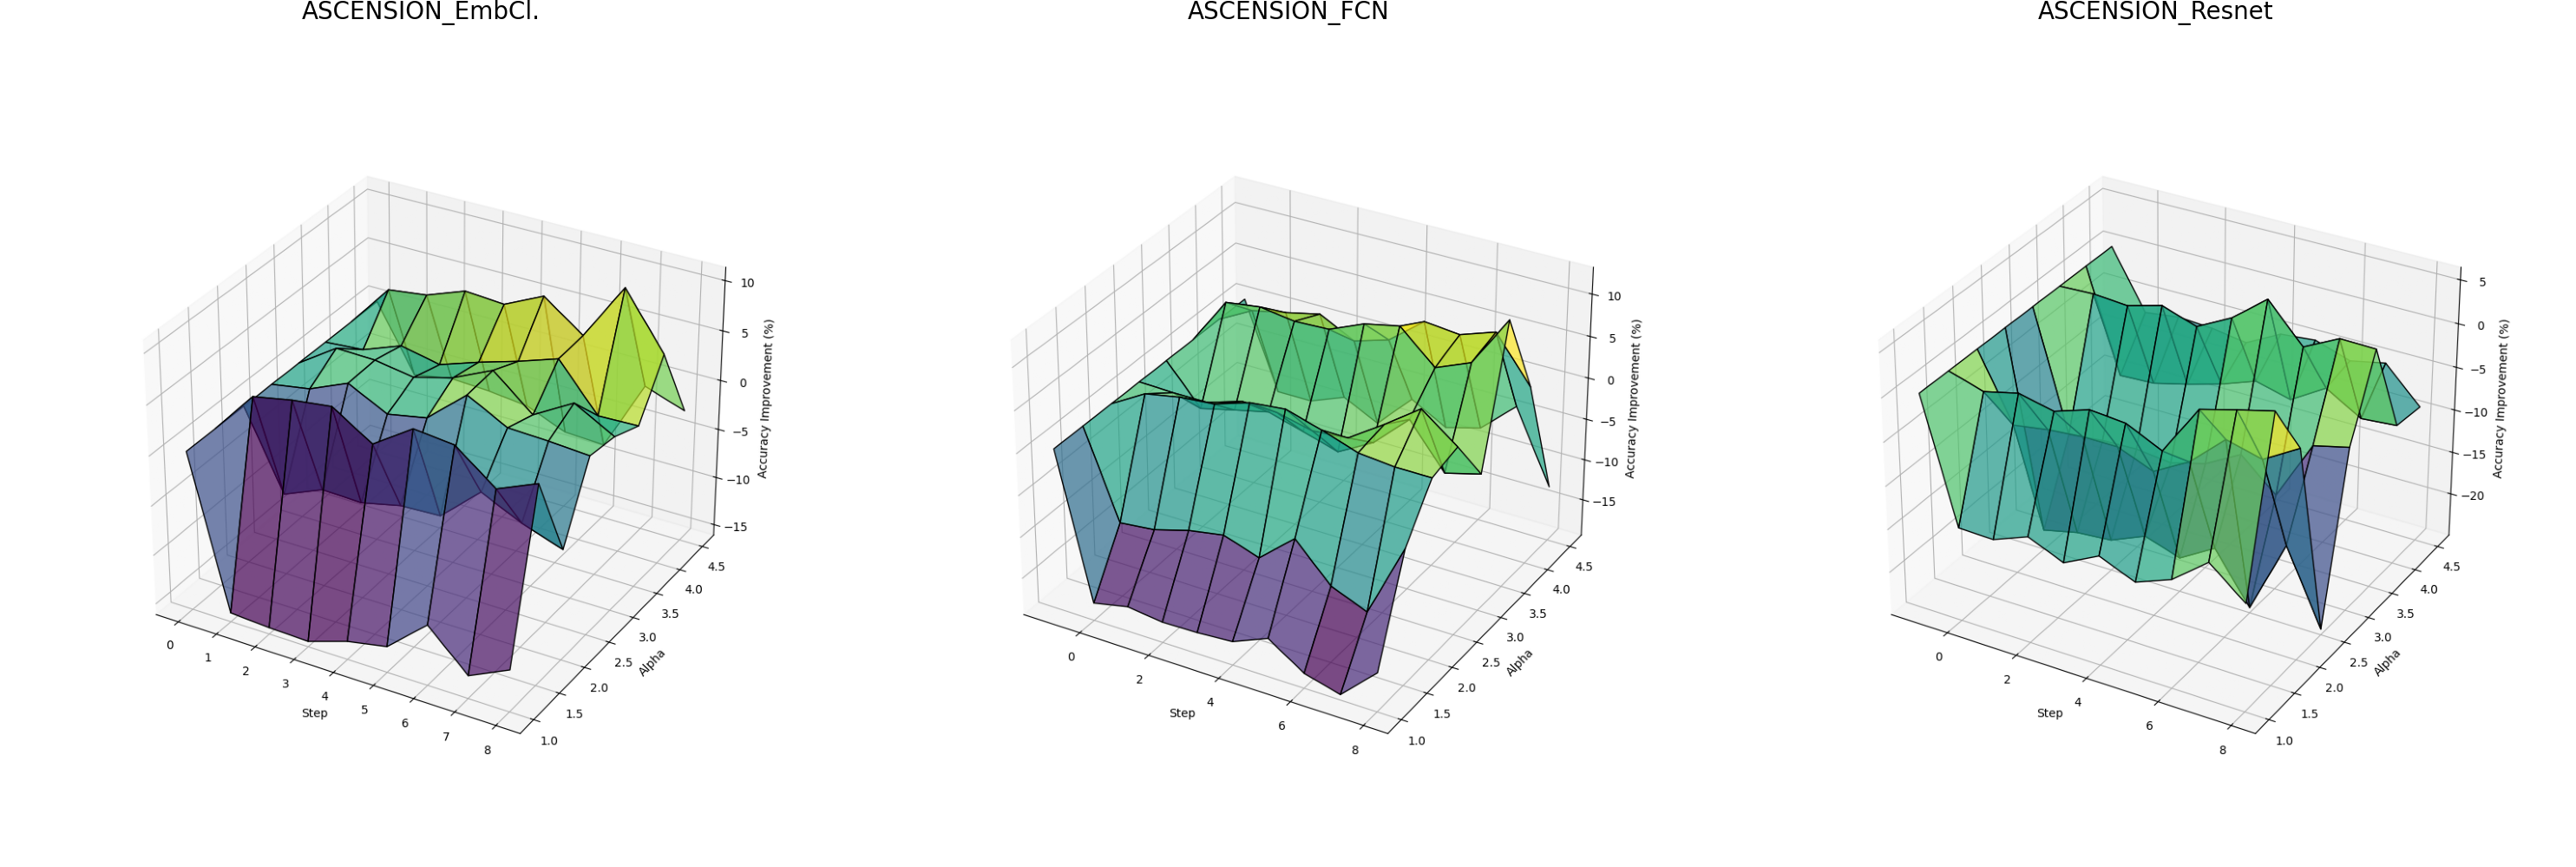
\includegraphics[width=\linewidth,clip=true,trim=0cm 3cm 0cm 5cm]{images/alpha_study_combined_EOGVerticalSignal.png}
    \caption{  \textbf{EOG:} Classifier performance against $\alpha$ and iteration count for \textbf{EOGVerticalSignal} datasets.}
    \label{fig:images/alpha_study_EOGVerticalSignal}
\end{figure}

\begin{figure}[h]
    \centering
      
    ASCENSION$_\text{Emb.}$ \hfill ASCENSION$_\text{FCN-Emb.}$ \hfill ASCENSION$_\text{ResNet-Emb.}$ \hspace{1cm}
    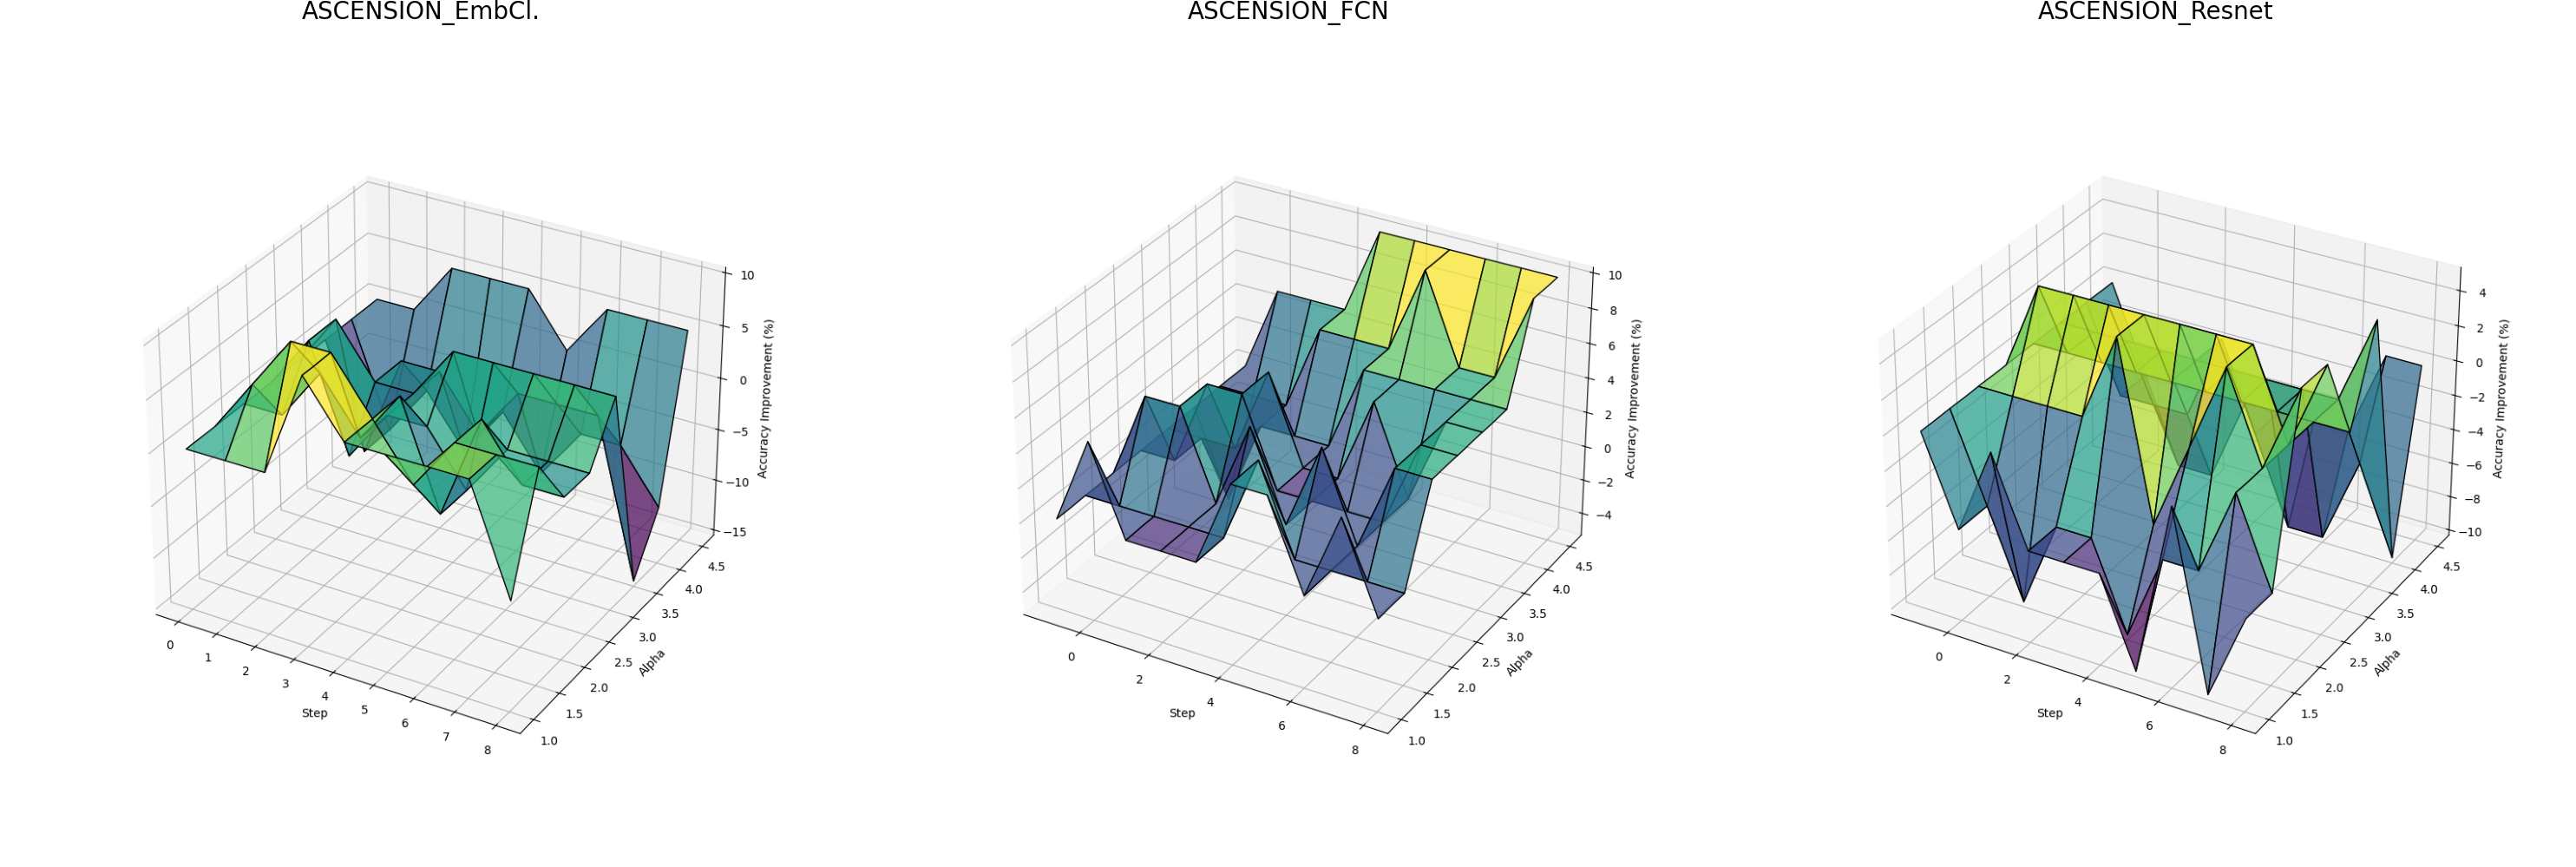
\includegraphics[width=\linewidth,clip=true,trim=0cm 3cm 0cm 5cm]{images/alpha_study_combined_BeetleFly.png}
    \caption{  \textbf{Image:} Classifier performance against $\alpha$ and iteration count for \textbf{BeetleFly} dataset.}
    \label{fig:images/alpha_study_BeetleFly}
\end{figure}


\begin{table*}[p]
\centering
 
\caption{Accuracy gain ($\overline{Acc}_{\Delta_1 Step}$) after first augmentation step per dataset for the $\alpha$-scaling mechanism and clustering loss ablation studies, along with best pair (iter., $\alpha$) identified per dataset, the train/test ratio (F23), and the train/test discrepancy}\label{Tab:app:Ablation_clustering_alpha} 

\setlength{\tabcolsep}{4pt} % Reduce space between columns

\scalebox{.9}{
\begin{tabular}{lr | r | lr | rrr}

\toprule
 &  & $\mathcal{L}_{\text{cluster}}$ ablation & \multicolumn{2}{c|}{$\alpha$-scaling ablation} & F23 & \multicolumn{2}{c}{Discrepancy}\\
\# & Dataset & $\overline{Acc}_{\Delta_1 Step}$ & (iter., $\alpha$) & Gain & Ratio & Disp$_{\text{Test}}$ & Disp$_{\text{Train}}$\\
 \midrule
D1 & ACSF1 & -0.01 & (1, 2) & -0.01 & 0.96 & $1.01\times10^{3}$ & $1.04\times10^{3}$ \\
D2 & Adiac & -0.01 & (1, 1) & -0.05 & 1.09 & $2.81\times10^{1}$ & $2.25\times10^{1}$ \\
D3 & ArrowHead & -0.05 & (1, 4) & 0.11 & 1.16 & $1.71\times10^{0}$ & $1.88\times10^{0}$ \\
D4 & BME & 0.03 & (1, 2) & -0.00 & 1.13 & $1.64\times10^{2}$	&	$1.26\times10^{2}$\\
D5 & Beef & 0.13 & (1, 3) & 0.27 & 0.94 & $6.40\times10^{1}$ & $6.78\times10^{1}$ \\
D6 & BeetleFly & 0.00 & (1, 1) & 0.32 & 0.89 & $5.79\times10^{1}$ & $5.30\times10^{1}$ \\
D7 & BirdChicken & -0.02 & (1, 1) & 0.00 & 1.30 & $5.28\times10^{1}$ & $5.47\times10^{1}$ \\
D8 & Car & 0.01 & (1, 4) & 0.00 & 1.51 & $3.94\times10^{2}$ & $3.95\times10^{2}$ \\
D9 & CBF & -0.02 & (1, 1) & 0.01 & 1.09 & $6.69\times10^{4}$ & $8.63\times10^{4}$ \\
D10 & ChlorineConcentration & 0.00 & (1, 3) & 0.00 & 1.05 & $9.02\times10^{1}$ & $9.00\times10^{1}$ \\
D11 & CinCECGTorso & -0.00 & (1, 3) & 0.00 & 1.24 & $1.41\times10^{1}$ & $1.40\times10^{1}$ \\
D12 & Coffee & -0.13 & (1, 4) & 0.03 & 1.07 & $8.05\times10^{0}$ & $8.45\times10^{0}$ \\
D13 & Computers & 0.02 & (1, 1) & -0.01 & 0.97 & $1.94\times10^{2}$ & $1.98\times10^{2}$ \\
D14 & Crop & -0.01 & (1, 4) & -0.00 & 1.00 & $1.28\times10^{4}$ & $1.35\times10^{4}$ \\
D15 & DistalPhalanxOutlineAgeGroup & 0.03 & (1, 1) & -0.01 & 1.21 & $6.78\times10^{1}$ & $6.71\times10^{1}$ \\
D16 & DistalPhalanxOutlineCorrect & 0.00 & (1, 2) & -0.00 & 0.96 & $5.31\times10^{0}$ & $6.94\times10^{0}$ \\
D17 & DistalPhalanxTW & -0.02 & (1, 2) & -0.00 & 1.04 & $2.07\times10^{1}$ & $2.07\times10^{1}$ \\
D18 & ECG200 & -0.01 & (1, 2) & 0.01 & 1.21 & $1.28\times10^{2}$ & $1.25\times10^{2}$ \\
D19 & ECG5000 & -0.00 & (1, 2) & 0.02 & 1.19 & $4.17\times10^{1}$ & $4.77\times10^{1}$ \\
D20 & ECGFiveDays & 0.00 & (1, 2) & -0.01 & 1.01 & $5.42\times10^{1}$ & $4.85\times10^{1}$ \\
D21 & EOGHorizontalSignal & 0.00 & (1, 4) & -0.00 & 1.18 & $3.01\times10^{1}$ & $2.65\times10^{1}$ \\
D22 & EOGVerticalSignal & -0.01 & (1, 3) & -0.00 & 0.77 & $6.38\times10^{3}$ & $5.62\times10^{3}$ \\
D23 & Earthquakes & -0.02 & (1, 3) & 0.01 & 1.00 & $1.31\times10^{2}$ & $1.24\times10^{2}$ \\
D24 & ElectricDevices & 0.01 & (1, 2) & -0.01 & 1.10 & $1.02\times10^{2}$ & $9.84\times10^{1}$ \\
D25 & EthanolLevel & -0.00 & (1, 3) & 0.00 & 0.87 & $3.18\times10^{1}$ & $2.10\times10^{1}$ \\
D26 & FaceAll & 0.02 & (1, 1) & 0.01 & 0.97 & $3.58\times10^{1}$ & $3.67\times10^{1}$ \\
D27 & FaceFour & -0.06 & (1, 1) & -0.02 & 1.04 & $5.44\times10^{1}$ & $5.14\times10^{1}$ \\
D28 & FacesUCR & -0.01 & (1, 1) & 0.00 & 1.12 & $1.20\times10^{3}$ & $1.08\times10^{3}$ \\
D29 & Fish & -0.04 & (1, 3) & 0.00 & 1.00 & $1.13\times10^{3}$ & $9.94\times10^{2}$ \\
D30 & FordA & -0.00 & (1, 2) & 0.00 & 0.99 & $3.73\times10^{3}$ & $3.83\times10^{3}$ \\
D31 & FordB & -0.01 & (1, 4) & -0.01  & 0.98 & $2.81\times10^{0}$ & $2.80\times10^{0}$ \\
D32 & FreezerRegularTrain & -0.00 & (1, 3) & 0.00 & 1.01 & $2.47\times10^{3}$ & $3.27\times10^{3}$ \\
D33 & FreezerSmallTrain & 0.03 & (1, 4) & 0.00 & 1.11 & $2.29\times10^{2}$ & $2.35\times10^{2}$ \\
D34 & GunPoint & -0.02 & (1, 2) & 0.00 & 1.04 & $3.83\times10^{2}$ & $3.91\times10^{2}$ \\
D35 & GunPointAgeSpan & -0.00 & (1, 1) & 0.00 & 1.00 & $5.50\times10^{0}$ & $4.90\times10^{0}$ \\
D36 & GunPointMaleVersusFemale & -0.01 & (1, 2) & 0.00 & 1.02 & $3.69\times10^{1}$ & $5.17\times10^{1}$ \\
D37 & GunPointOldVersusYoung & 0.00 & (1, 1) & -0.00 & 1.02 & $5.70\times10^{2}$ & $6.35\times10^{2}$ \\
D38 & Ham & -0.03 & (1, 3) & 0.00 & 1.07 & $4.23\times10^{2}$ & $3.75\times10^{2}$ \\
D39 & HandOutlines & -0.00 & (1, 2) & 0.01 & 0.46 & $1.50\times10^{2}$ & $1.39\times10^{2}$ \\
D40 & Haptics & -0.01 & (1, 4) & 0.01 & 1.08 & $3.27\times10^{1}$ & $2.98\times10^{1}$ \\
D41 & Herring & 0.02 & (1, 2) & -0.01 & 1.01 & $1.02\times10^{1}$ & $1.07\times10^{1}$ \\
D42 & HouseTwenty & 0.00 & (1, 2) & 0.01 & 0.99 & $2.44\times10^{0}$ & $2.79\times10^{0}$ \\
D43 & InlineSkate & -0.02 & (1, 2) & 0.00 & 1.07 & $8.25\times10^{0}$ & $6.80\times10^{0}$ \\
D44 & InsectWingbeatSound & -0.00 & (1, 1) & 0.00 & 1.06 & $7.54\times10^{2}$ & $7.85\times10^{2}$ \\
D45 & InsectEPGRegularTrain & 0.00 & (3, 1) & 0.00 & 1.26 & $1.88\times10^{1}$ & $1.94\times10^{1}$ \\
D46 & InsectEPGSmallTrain & 0.00 & (1, 1) & 0.00 & 1.10 & $1.63\times10^{2}$ & $1.64\times10^{2}$ \\
D47 & ItalyPowerDemand & -0.00 & (1, 3) & 0.00 & 0.95 & $2.75\times10^{0}$ & $2.92\times10^{0}$ \\
D48 & LargeKitchenAppliances & -0.01 & (1, 1) & 0.00 & 1.01 & $3.68\times10^{1}$ & $3.08\times10^{1}$ \\
 D49 & Lightning2 & -0.04 & (1, 2) & 0.01 & 1.02 & $5.96\times10^{1}$ & $1.31\times10^{2}$ \\
D50 & Lightning7 & -0.04 & (1, 2) & -0.00 & 0.94 & $3.32\times10^{1}$ & $3.80\times10^{1}$ \\
 D51 & Mallat & 0.01 & (1, 4) & 0.00 & 1.11 & $2.40\times10^{1}$ & $2.32\times10^{1}$ \\
D52 & Meat & -0.02 & (1, 3) & -0.02 & 0.94 & $2.80\times10^{3}$ & $1.35\times10^{3}$ \\
D53 & MedicalImages & -0.01 & (1, 2) & -0.01 & 1.00 & $7.57\times10^{1}$ & $8.10\times10^{1}$ \\
\bottomrule
\end{tabular}
}
\end{table*}

\setcounter{table}{16}
\begin{table*}[p]
\centering
 
\caption{Accuracy gain ($\overline{Acc}_{\Delta_1 Step}$) after first augmentation step per dataset for the $\alpha$-scaling mechanism and clustering loss ablation studies, along with best pair (iter., $\alpha$) identified per dataset, the train/test ratio (F23), and the train/test discrepancy}

\setlength{\tabcolsep}{4pt} % Reduce space between columns

\scalebox{.9}{
\begin{tabular}{lr | r | lr | rrr}

\toprule
 &  & $\mathcal{L}_{\text{cluster}}$ ablation & \multicolumn{2}{c|}{$\alpha$-scaling ablation} & F23 & \multicolumn{2}{c}{Discrepancy}\\
\# & Dataset & $\overline{Acc}_{\Delta_1 Step}$ & (iter., $\alpha$) & Gain & Ratio & Disp$_{\text{Test}}$ & Disp$_{\text{Train}}$\\
 \midrule
D54 & MiddlePhalanxOutlineAgeGroup & 0.01 & (1, 3) & -0.01 & 1.12 & $2.70\times10^{1}$ & $2.24\times10^{1}$ \\
D55 & MiddlePhalanxOutlineCorrect & -0.02 & (1, 2) & -0.01 & 0.77 & $1.01\times10^{6}$ & $1.02\times10^{6}$ \\
D56 & MiddlePhalanxTW & -0.03 & (1, 3) & 0.00 & 0.94 & $4.74\times10^{0}$ & $5.02\times10^{0}$ \\
D57 & MixedShapesRegularTrain & 0.00 & (1, 2) & 0.01 & 0.98 & $4.20\times10^{2}$ & $4.76\times10^{2}$ \\
D58 & MixedShapesSmallTrain & 0.01 & (1, 4) & 0.01 & 1.19 & $1.59\times10^{2}$ & $1.55\times10^{2}$ \\
D59 & MoteStrain & 0.00 & (1, 2) & -0.00 & 0.96 & $3.27\times10^{1}$ & $2.60\times10^{1}$ \\
D60 & NonInvasiveFetalECGThorax1 & -0.00 & (1, 1) & -0.00 & 0.98 & $1.31\times10^{2}$ & $1.33\times10^{2}$ \\
D61 & NonInvasiveFetalECGThorax2 & 0.01 & (1, 1) & 0.01 & 0.97 & $2.52\times10^{0}$ & $2.42\times10^{0}$ \\
D62 & OSULeaf & 0.01 & (1, 4) & 0.01 & 0.98 & $8.85\times10^{3}$ & $6.43\times10^{3}$ \\
D63 & OliveOil & 0.00 & (1, 1) & 0.00 & 0.91 & $5.64\times10^{0}$ & $5.94\times10^{0}$ \\
D64 & PhalangesOutlinesCorrect & -0.00 & (1, 2) & -0.00 & 0.95 & $2.02\times10^{1}$ & $2.00\times10^{1}$ \\
D65 & Plane & 0.00 & (1, 1) & 0.00 & 0.94 & $9.58\times10^{1}$ & $1.01\times10^{2}$ \\
D66 & PowerCons & 0.00 & (1, 1) & 0.00 & 1.02 & $2.07\times10^{4}$ & $1.63\times10^{4}$ \\
D67 & ProximalPhalanxOutlineAgeGroup & -0.02 & (1, 1) & -0.02 & 0.94 & $4.70\times10^{2}$ & $7.09\times10^{2}$ \\
D68 & ProximalPhalanxOutlineCorrect & -0.01 & (1, 1) & -0.01  & 0.87 & $1.34\times10^{1}$ & $1.48\times10^{1}$ \\
D69 & ProximalPhalanxTW & -0.00 & (1, 1) & -0.00 & 0.94 & $1.39\times10^{4}$ & $1.36\times10^{4}$ \\
D70 & RefrigerationDevices & -0.01 & (1, 2) & -0.01 & 1.05 & $4.23\times10^{1}$ & $4.01\times10^{1}$ \\
D71 & Rock & -0.01 & (1, 4) & -0.01 & 1.27 & $1.16\times10^{2}$ & $1.11\times10^{2}$ \\
D72 & ScreenType & 0.02 & (1, 2) & 0.02 & 0.88 & $2.18\times10^{2}$ & $2.46\times10^{2}$ \\
D73 & SemgHandGenderCh2 & 0.01 & (1, 3) & 0.01 & 0.97 & $1.47\times10^{2}$ & $1.53\times10^{2}$ \\
D74 & SemgHandMovementCh2 & -0.03 & (1, 1) & -0.03 & 1.00 & $1.23\times10^{4}$ & $1.24\times10^{4}$ \\
D75 & SemgHandSubjectCh2 & -0.01 & (1, 1) & -0.01 & 0.95 & $5.14\times10^{1}$ & $5.28\times10^{1}$ \\
D76 & ShapeletSim & 0.00 & (1, 1) & -0.01 & 1.14 & $1.41\times10^{4}$ & $1.46\times10^{4}$ \\
D77 & ShapesAll & -0.02 & (1, 1) & 0.05 & 0.94 & $4.40\times10^{1}$ & $3.95\times10^{1}$ \\
D78 & SmallKitchenAppliances & 0.01 & (1, 1) & -0.00 & 0.99 & $2.49\times10^{1}$ & $2.61\times10^{1}$ \\
D79 & SmoothSubspace & 0.01 & (1, 2) & -0.00 & 1.04 & $4.86\times10^{1}$ & $3.19\times10^{1}$ \\
D80 & SonyAIBORobotSurface1 & -0.00 & (1, 3) & -0.00 & 1.00 & $8.36\times10^{0}$ & $8.36\times10^{0}$ \\
D81 & SonyAIBORobotSurface2 & -0.01 & (1, 1) & -0.01 & 1.18 & $2.80\times10^{1}$ & $2.36\times10^{1}$ \\
D82 & StarlightCurves & -0.01 & (1, 2) & -0.01 & 1.05 & $5.40\times10^{4}$ & $4.59\times10^{4}$ \\
D83 & Strawberry & -0.01 & (1, 1) & -0.01 & 0.91 & $1.59\times10^{2}$ & $1.56\times10^{2}$ \\
D84 & SwedishLeaf & -0.01 & (1, 1) & -0.01 & 0.96 & $4.69\times10^{2}$ & $4.37\times10^{2}$ \\
D85 & Symbols & -0.02 & (1, 3) & -0.02 & 1.53 & $1.23\times10^{1}$ & $3.72\times10^{0}$ \\
D86 & SyntheticControl & 0.00 & (1, 1) & 0.00 & 1.02 & $2.29\times10^{2}$ & $1.92\times10^{2}$ \\
D87 & ToeSegmentation1 & -0.04 & (1, 1) & -0.04 & 1.18 & $2.19\times10^{2}$ & $2.16\times10^{2}$ \\
D88 & ToeSegmentation2 & 0.02 & (1, 1) & 0.02 & 0.97 & $2.03\times10^{2}$ & $1.72\times10^{2}$ \\
D89 & Trace & -0.01 & (1, 1) & -0.01 & 0.88 & $4.46\times10^{3}$ & $4.41\times10^{3}$ \\
D90 & TwoLeadECG & 0.01 & (1, 3) & 0.01 & 1.00 & $2.28\times10^{1}$ & $2.32\times10^{1}$ \\
D91 & TwoPatterns & -0.01 & (1, 1) & -0.01 & 1.00 & $5.83\times10^{2}$ & $3.90\times10^{2}$ \\
D92 & UMD & 0.02 & (1, 1) & 0.02 &  0.97 &$1.89\times10^{1}$ & $1.89\times10^{1}$ \\
D93 & UWaveGestureLibraryAll & -0.01 & (1, 3) & -0.01 & 1.04 & $5.73\times10^{1}$ & $5.46\times10^{1}$ \\
D94 & UWaveGestureLibraryX & -0.00 & (1, 1) & -0.00 & 1.02 & $6.81\times10^{1}$ & $6.67\times10^{1}$ \\
D95 & UWaveGestureLibraryY & 0.01 & (1, 2) & 0.01 & 1.05 & $2.00\times10^{1}$ & $1.73\times10^{1}$ \\
D96 & UWaveGestureLibraryZ & -0.01 & (1, 1) & -0.01 & 1.06 & $8.64\times10^{0}$ & $9.18\times10^{0}$ \\
D97 & Wafer & -0.00 & (1, 3) & -0.00 & 1.12 & $2.24\times10^{2}$ & $2.30\times10^{2}$ \\
D98 & Wine & 0.01 & (1, 4) & 0.04 & 0.87 & $3.34\times10^{4}$ & $3.33\times10^{4}$ \\
D99 & WordSynonyms & -0.01 & (1, 4) & -0.01 & 1.11 & $4.32\times10^{3}$ & $5.08\times10^{3}$ \\
D100 & Worms & -0.02 & (1, 2) & -0.01 & 0.89 & $1.13\times10^{2}$ & $1.00\times10^{2}$ \\
D101 & WormsTwoClass & -0.03 & (1, 2) & -0.03 & 0.93 & $4.09\times10^{1}$ & $4.26\times10^{1}$ \\
D102 & Yoga & -0.02 & (1, 3) & -0.02 & 1.02 & $3.02\times10^{4}$ & $2.97\times10^{4}$ \\

  
\bottomrule
\end{tabular}
}
\end{table*}




% \begin{table*}[t]
% \centering
 
% \caption{Accuracy gain ($\overline{Acc}_{\Delta_1 Step}$) after first augmentation step per dataset for the $\alpha$-scaling mechanism and clustering loss ablation studies, along with best pair ( iter., $\alpha$) identified per dataset}


% \scalebox{.85}{
% \begin{tabular}{lr | r | rr | rrr}

% \toprule
%  &  & $\mathcal{L}_{\text{cluster}}$ ablation & \multicolumn{2}{c|}{$\alpha$-scaling ablation} & F23 & \multicolumn{2}{c}{Discrepancy}\\
% \# & Dataset & $\overline{Acc}_{\Delta_1 Step}$ & ( iter., $\alpha$) & $\overline{Acc}_{\Delta_1 Step}$ & Ratio & Disp$_{\text{Test}}$ & Disp$_{\text{Train}}$\\
%  \midrule
% D90 & TwoLeadECG & 0.01 & (1, 3) & 0.01 & 1.00 & $2.28\times10^{1}$ & $2.32\times10^{1}$ \\
% D91 & TwoPatterns & -0.01 & (1, 1) & -0.01 & 1.00 & $5.83\times10^{2}$ & $3.90\times10^{2}$ \\
% D92 & UMD & 0.02 & (1, 1) & 0.02 &  0.97 &$1.89\times10^{1}$ & $1.89\times10^{1}$ \\
% D93 & UWaveGestureLibraryAll & -0.01 & (1, 3) & -0.01 & 1.04 & $5.73\times10^{1}$ & $5.46\times10^{1}$ \\
% D94 & UWaveGestureLibraryX & -0.00 & (1, 1) & -0.00 & 1.02 & $6.81\times10^{1}$ & $6.67\times10^{1}$ \\
% D95 & UWaveGestureLibraryY & 0.01 & (1, 2) & 0.01 & 1.05 & $2.00\times10^{1}$ & $1.73\times10^{1}$ \\
% D96 & UWaveGestureLibraryZ & -0.01 & (1, 1) & -0.01 & 1.06 & $8.64\times10^{0}$ & $9.18\times10^{0}$ \\
% D97 & Wafer & -0.00 & (1, 3) & -0.00 & 1.12 & $2.24\times10^{2}$ & $2.30\times10^{2}$ \\
% D98 & Wine & 0.01 & (1, 4) & 0.04 & 0.87 & $3.34\times10^{4}$ & $3.33\times10^{4}$ \\
% D99 & WordSynonyms & -0.01 & (1, 4) & -0.01 & 1.11 & $4.32\times10^{3}$ & $5.08\times10^{3}$ \\
% D100 & Worms & -0.02 & (1, 2) & -0.01 & 0.89 & $1.13\times10^{2}$ & $1.00\times10^{2}$ \\
% D101 & WormsTwoClass & -0.03 & (1, 2) & -0.03 & 0.93 & $4.09\times10^{1}$ & $4.26\times10^{1}$ \\
% D102 & Yoga & -0.02 & (1, 3) & -0.02 & 1.02 & $3.02\times10^{4}$ & $2.97\times10^{4}$ \\


  
% \bottomrule
% \end{tabular}
% }
% \end{table*}
\newpage


%\textcolor{red}{INtroduce table column 1 (best pair); column ($\overline{Acc}_{\Delta_1 Step}$) + Comments (Q1, median, Q3)}




% % ECG
% \begin{figure}[H]
%     \centering
%       
%     \hspace{1.5cm} ASCENSION$_\text{Emb.}$ \hfill ASCENSION$_\text{FCN-Emb.}$ \hfill ASCENSION$_\text{ResNet-Emb.}$ \hspace{1cm}
    
%     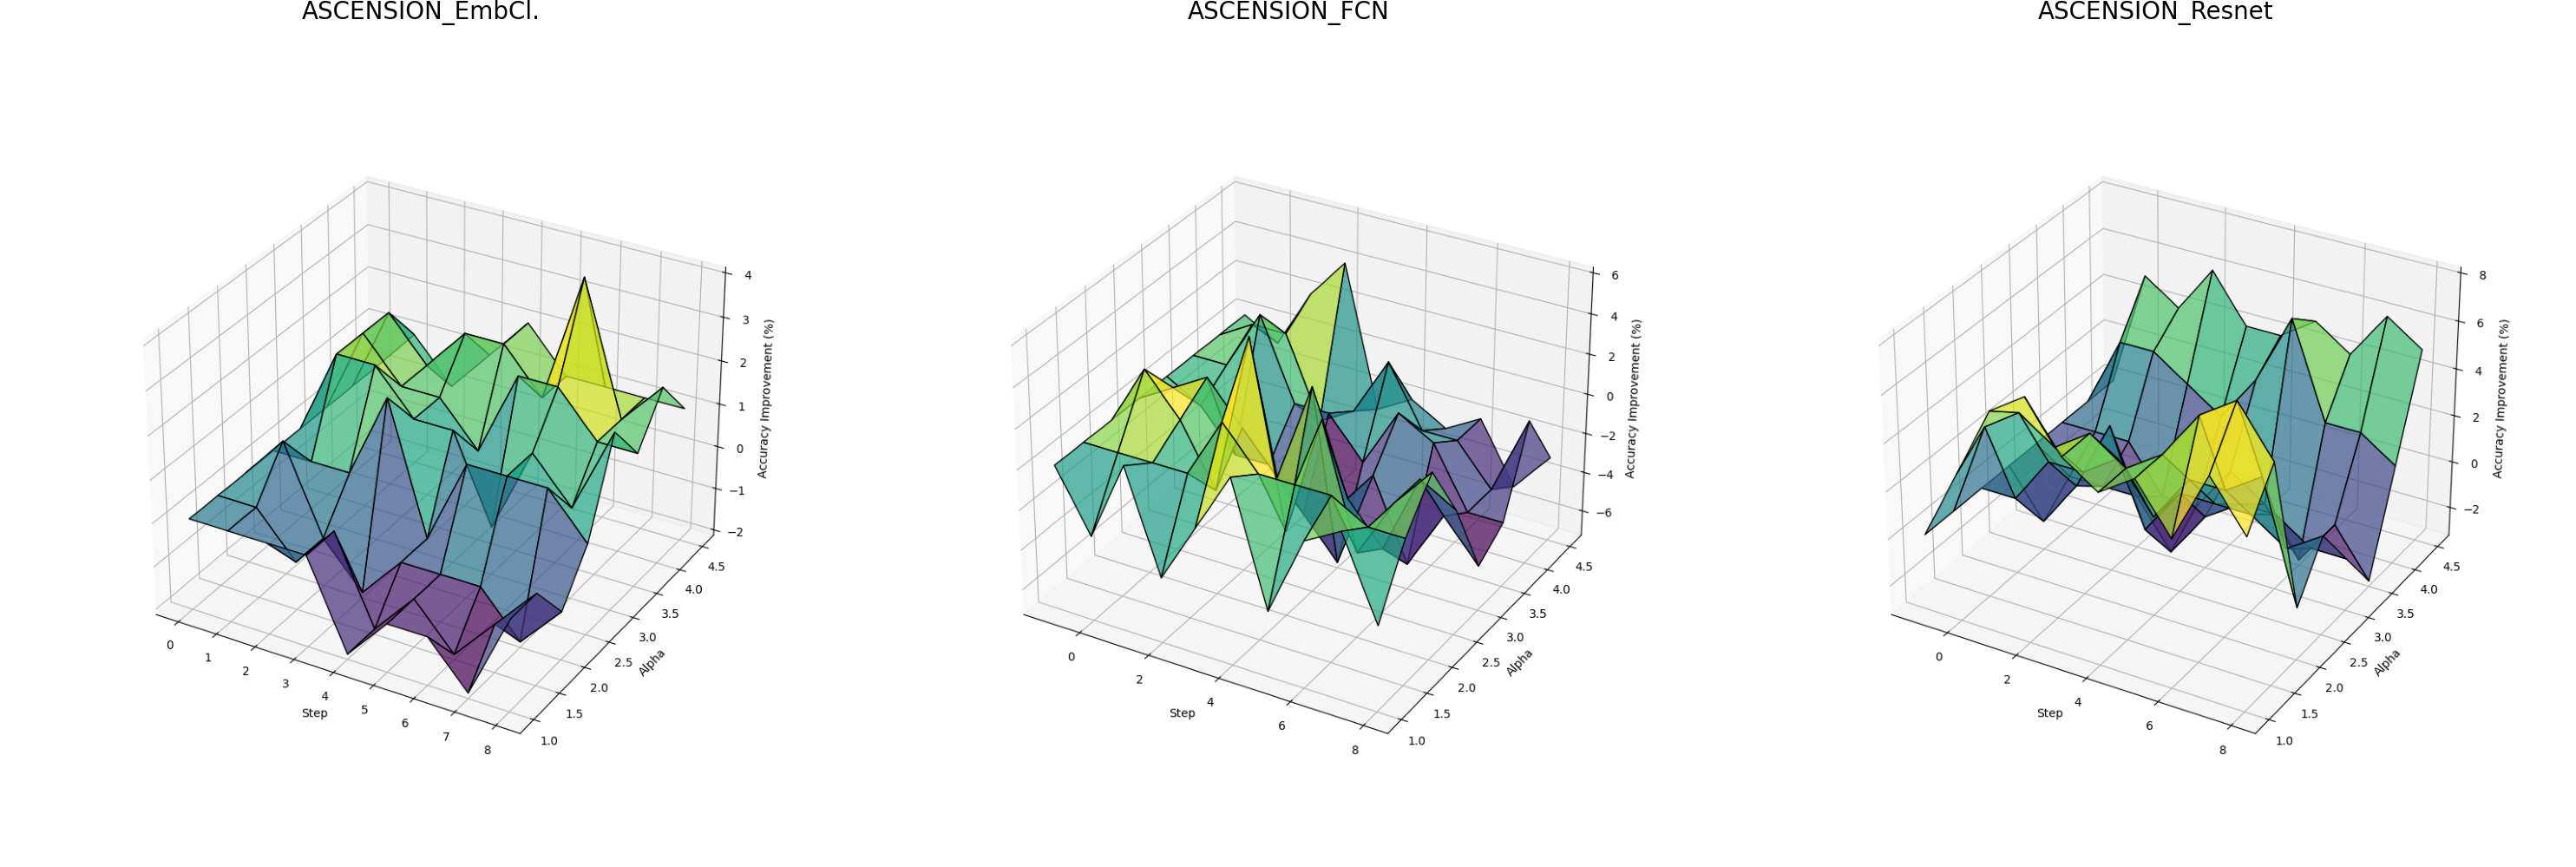
\includegraphics[width=\linewidth,clip=true,trim=0cm 3cm 0cm 5cm]{images/alpha_study_combined_ECG200.png}
    
%     \caption{\textbf{ECG:} Classifier performance against $\alpha$ and iteration number for \textbf{ECG200} dataset.}
%     \label{fig:images/alpha_study_ECG200}
% \end{figure}

% EOG


% % Hemodynamics
% \begin{figure}[H]
%     \centering
%       
%     \hspace{1.5cm} ASCENSION$_\text{Emb.}$ \hfill ASCENSION$_\text{FCN-Emb.}$ \hfill ASCENSION$_\text{ResNet-Emb.}$ \hspace{1cm}
%     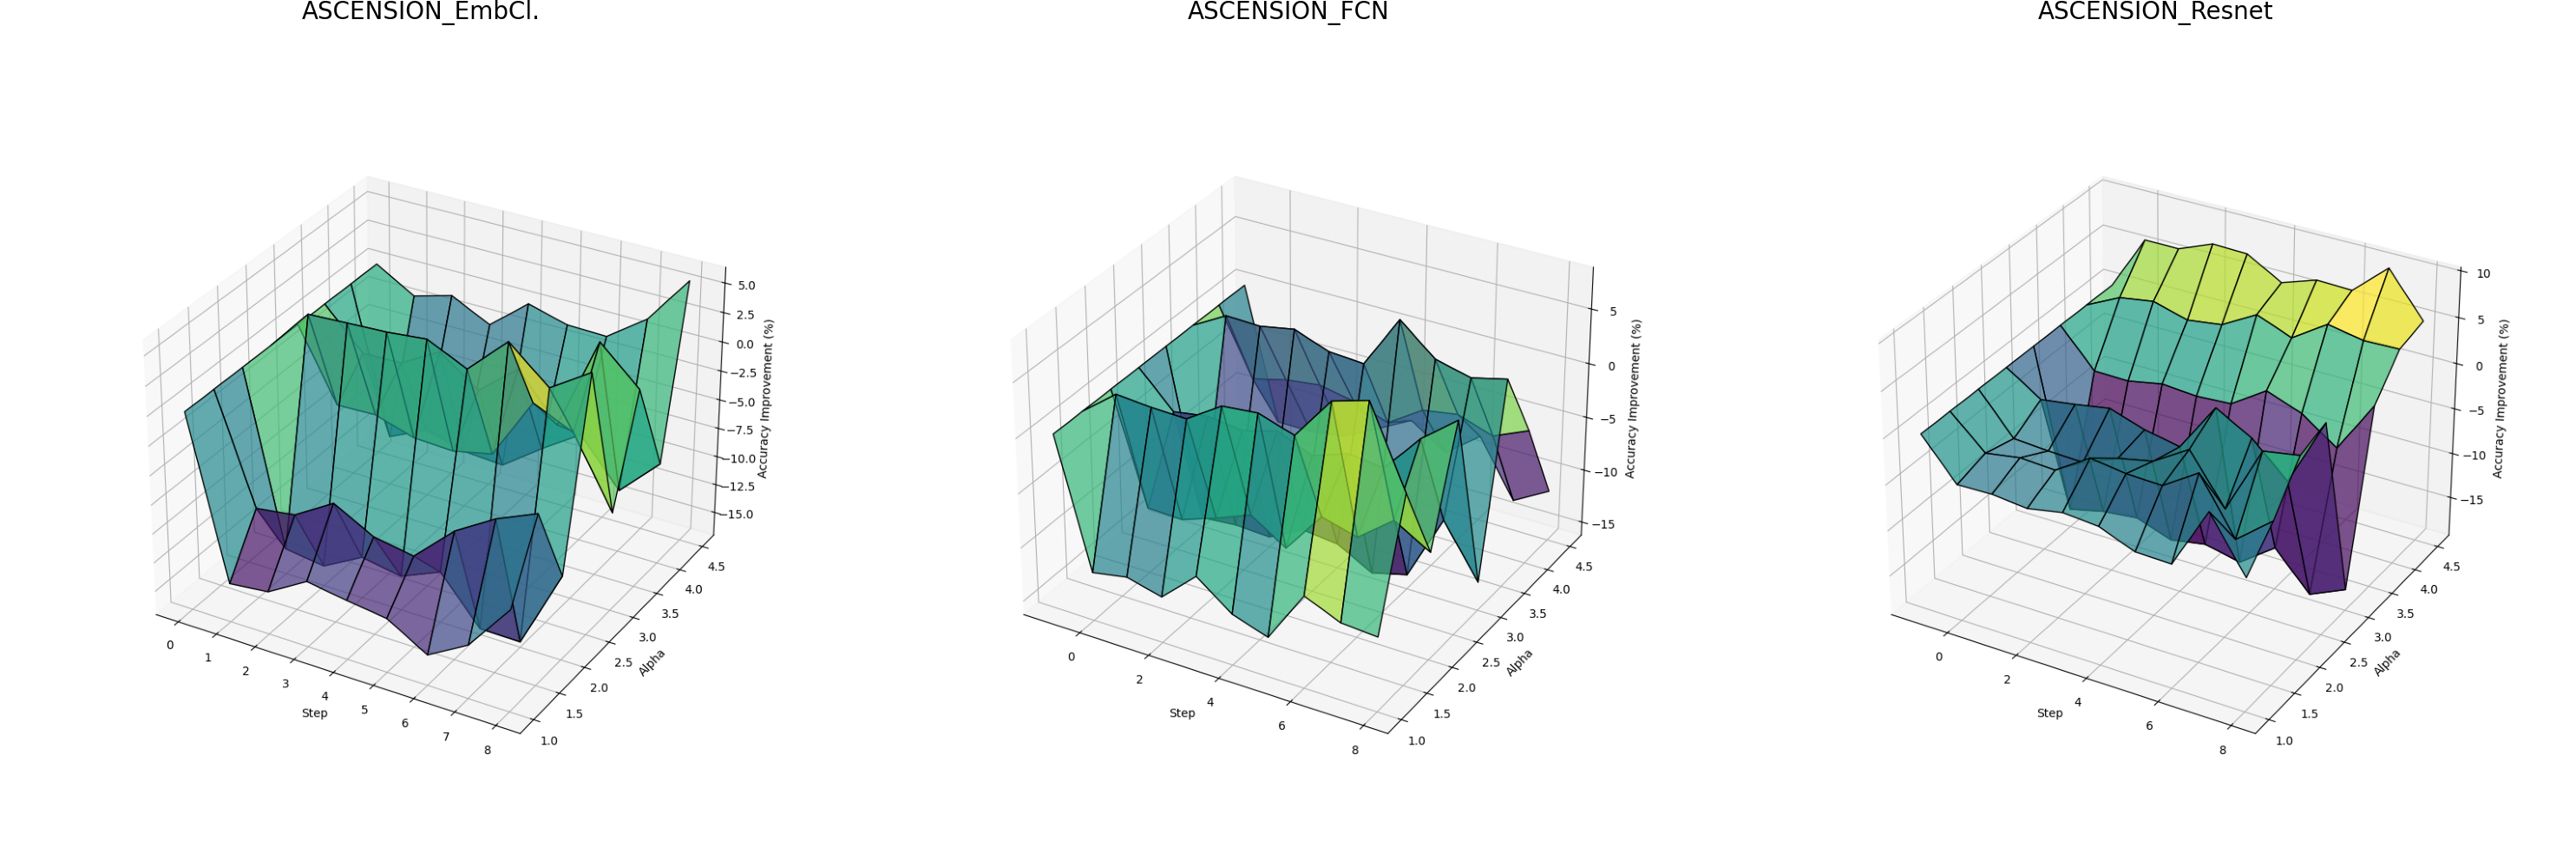
\includegraphics[width=\linewidth,clip=true,trim=0cm 3cm 0cm 5cm]{images/alpha_study_combined_PigArtPressure.png}
%     \caption{\textbf{Hemodynamics:} Classifier performance against $\alpha$ and iterations for \textbf{PigArtPressure}. }
%     \label{fig:images/alpha_study_PigArtPressure}
% \end{figure}

% Image


% % Motion
% \begin{figure}[H]
%     \centering
%       
%     \hspace{1.5cm} ASCENSION$_\text{Emb.}$ \hfill ASCENSION$_\text{FCN-Emb.}$ \hfill ASCENSION$_\text{ResNet-Emb.}$ \hspace{1cm}
%     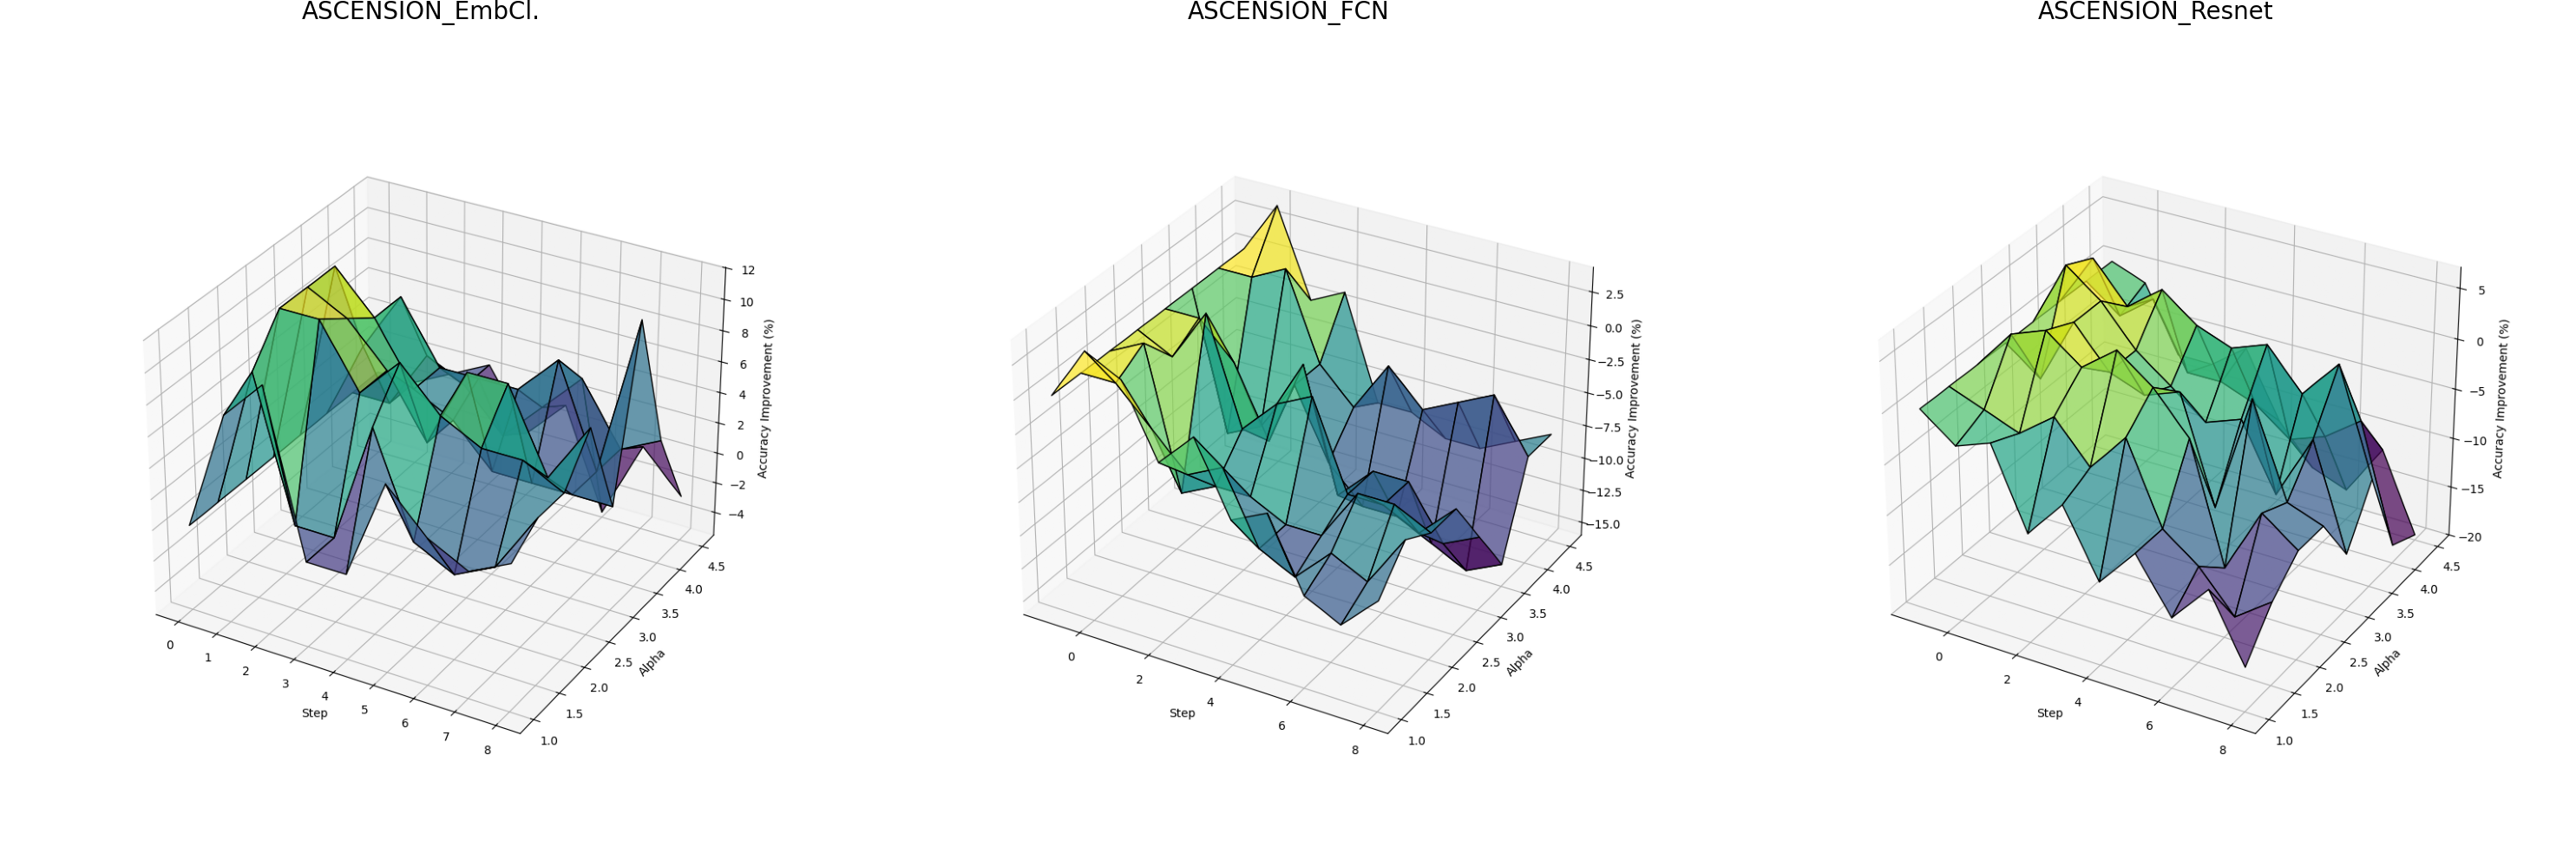
\includegraphics[width=\linewidth,clip=true,trim=0cm 3cm 0cm 5cm]{images/alpha_study_combined_Worms.png}
%     \caption{\textbf{Motion:} Classifier performance against $\alpha$ and iteration number for \textbf{Worms} dataset.}
%     \label{fig:images/alpha_study_Worms}
% \end{figure}

% % Sensor
% \begin{figure}[H]
%     \centering
%       
%     \hspace{1.5cm} ASCENSION$_\text{Emb.}$ \hfill ASCENSION$_\text{FCN-Emb.}$ \hfill ASCENSION$_\text{ResNet-Emb.}$ \hspace{1cm}
%     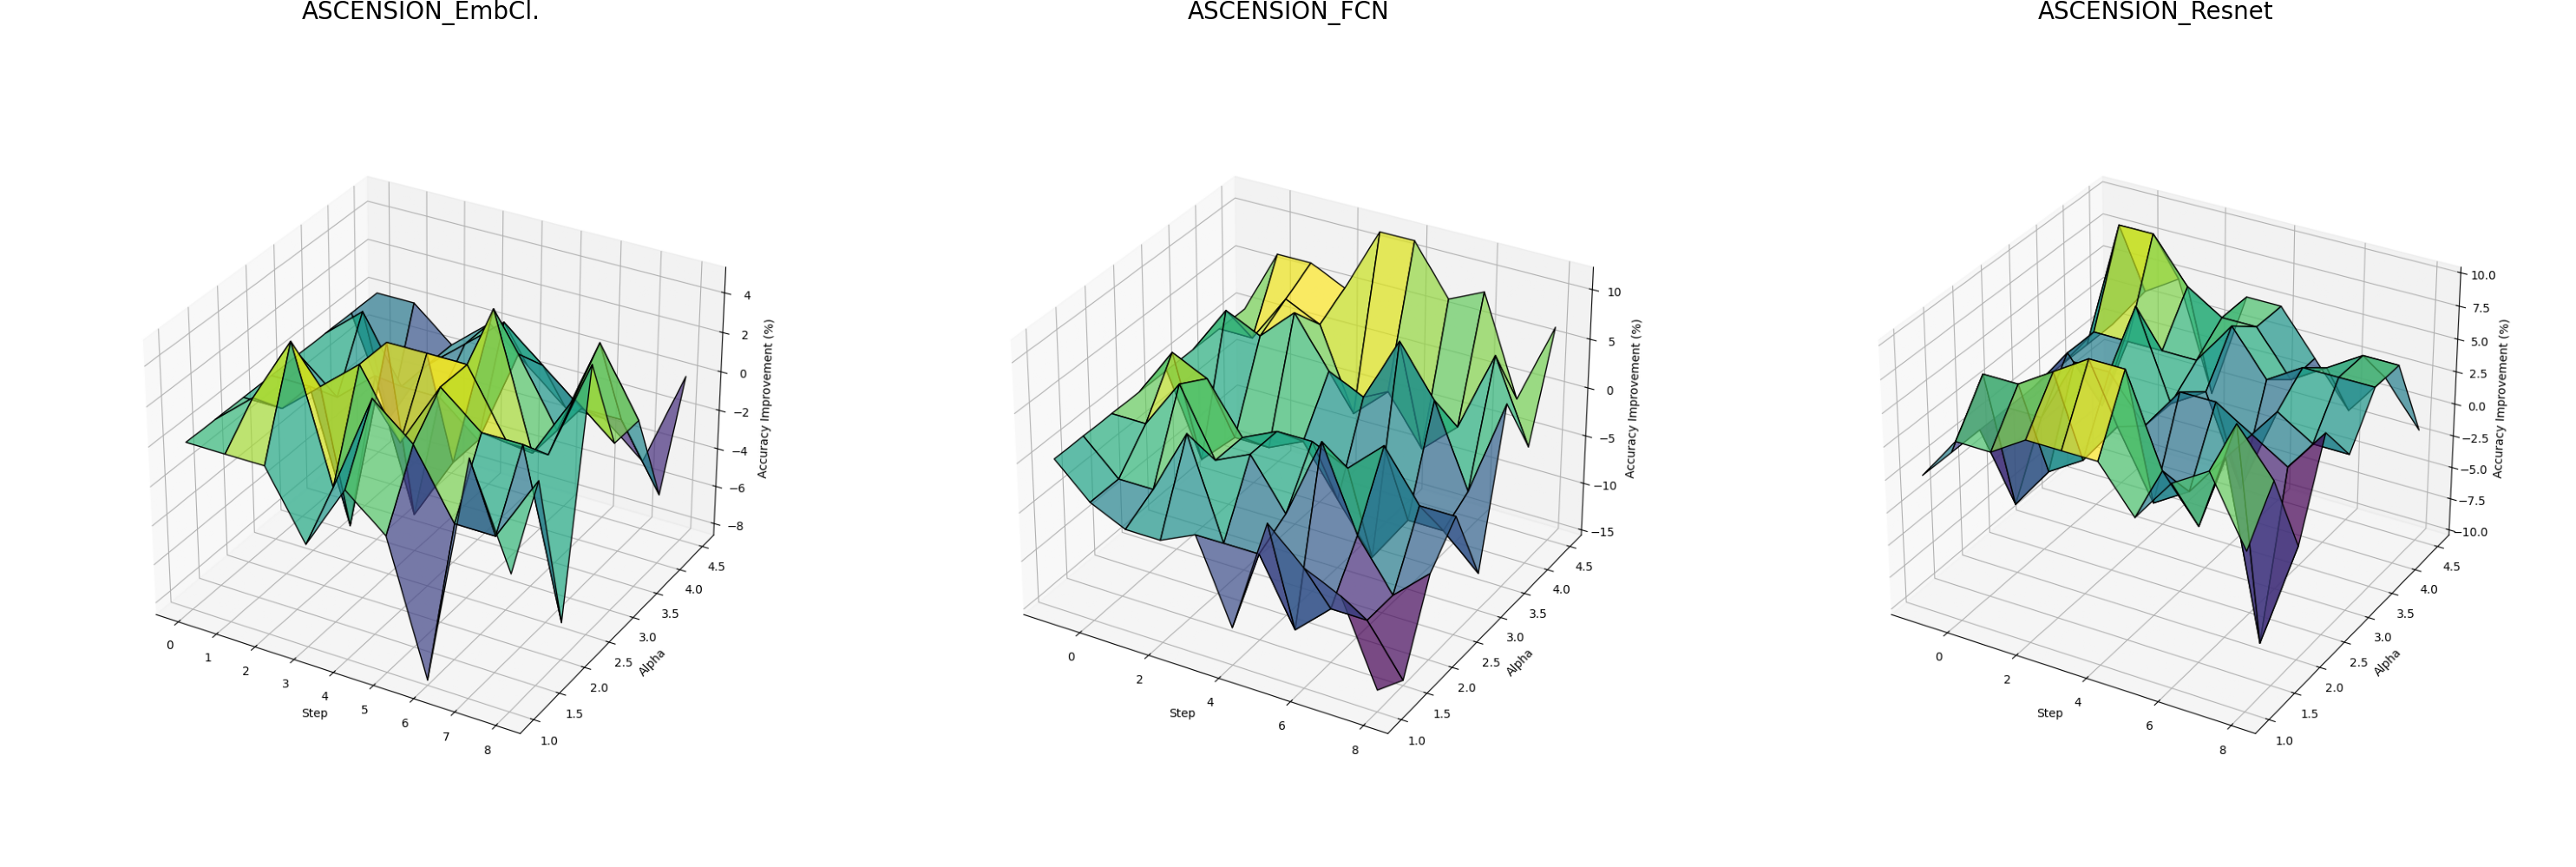
\includegraphics[width=\linewidth,clip=true,trim=0cm 3cm 0cm 5cm]{images/alpha_study_combined_Car.png}
%     \caption{\textbf{Sensor:} Classifier performance against $\alpha$ and iteration number for \textbf{Car} dataset.}
%     \label{fig:images/alpha_study_Car}
% \end{figure}

% % Simulated
% \begin{figure}[H]
%     \centering
%       
%     \hspace{1.5cm} ASCENSION$_\text{Emb.}$ \hfill ASCENSION$_\text{FCN-Emb.}$ \hfill ASCENSION$_\text{ResNet-Emb.}$ \hspace{1cm}
%     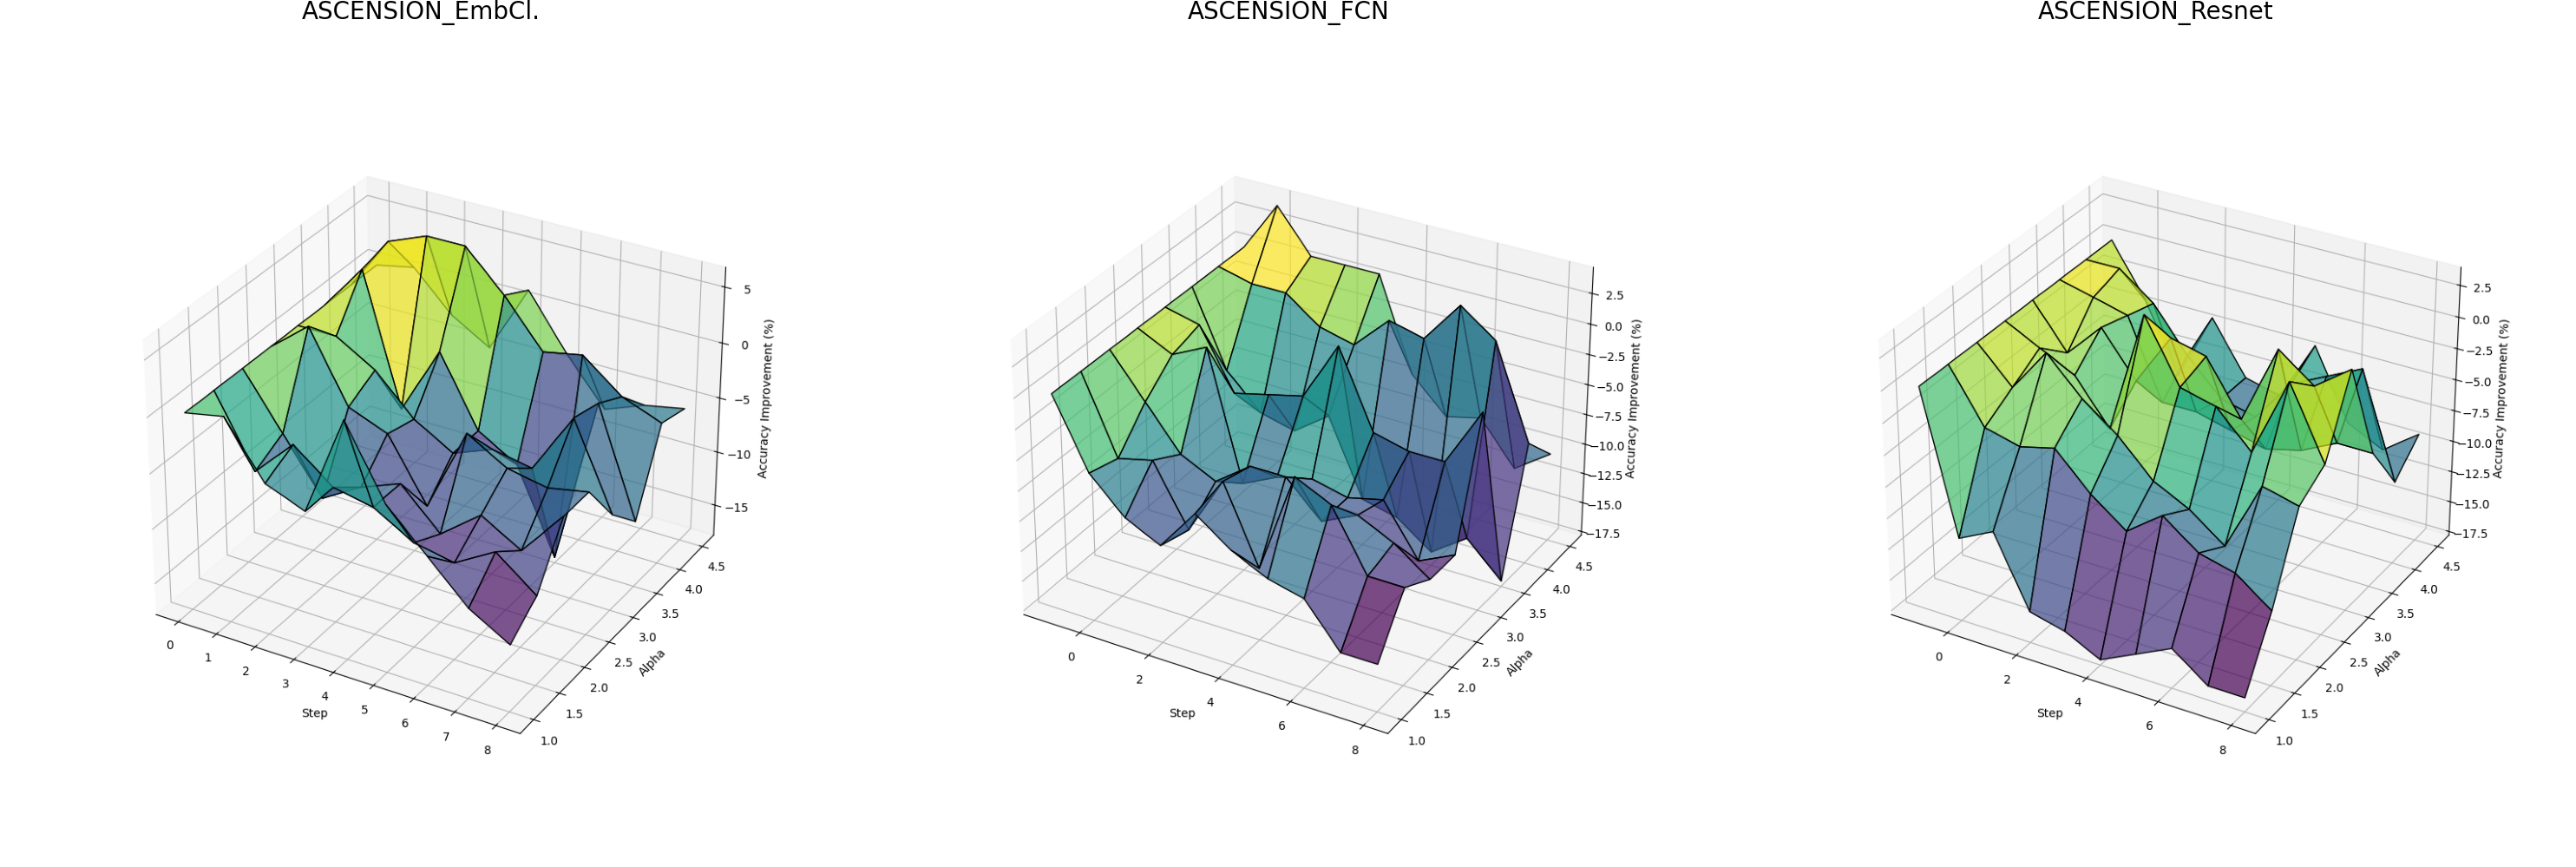
\includegraphics[width=\linewidth,clip=true,trim=0cm 3cm 0cm 5cm]{images/alpha_study_combined_UMD.png}
%     \caption{\textbf{Simulated:} Classifier performance against $\alpha$ and iteration number for \textbf{UMD} dataset.}
%     \label{fig:images/alpha_study_UMD}
% \end{figure}

% % Spectro
% \begin{figure}[H]
%     \centering
%       
%     \hspace{1.5cm} ASCENSION$_\text{Emb.}$ \hfill ASCENSION$_\text{FCN-Emb.}$ \hfill ASCENSION$_\text{ResNet-Emb.}$ \hspace{1cm}
%     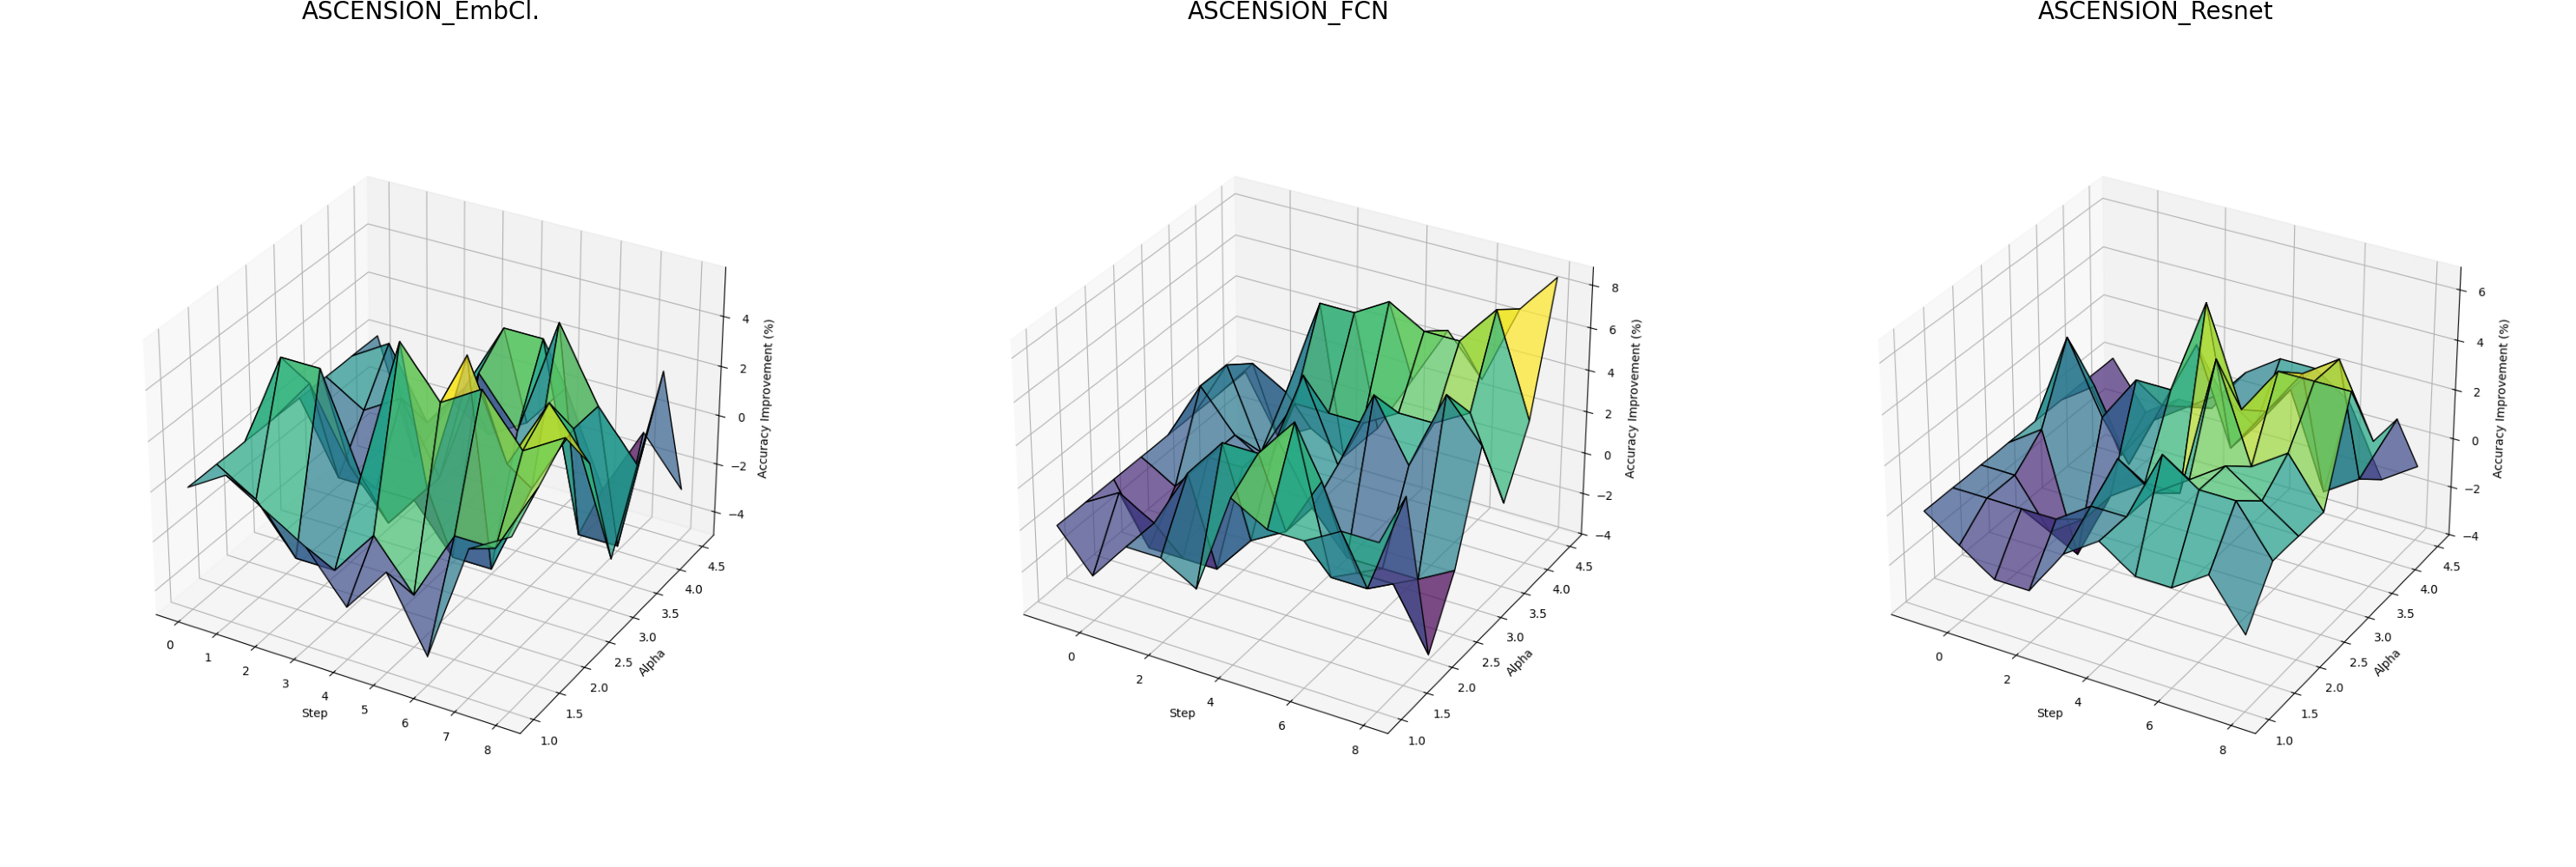
\includegraphics[width=\linewidth,clip=true,trim=0cm 3cm 0cm 5cm]{images/alpha_study_combined_Ham.png}
%     \caption{\textbf{Spectro:} Classifier performance against $\alpha$ and iteration number for \textbf{Ham} dataset.}
%     \label{fig:images/alpha_study_Ham}
% \end{figure}

% % Spectrum
% \begin{figure}[H]
%     \centering
%           
%     \hspace{1.5cm} ASCENSION$_\text{Emb.}$ \hfill ASCENSION$_\text{FCN-Emb.}$ \hfill ASCENSION$_\text{ResNet-Emb.}$ \hspace{1cm}
    
%     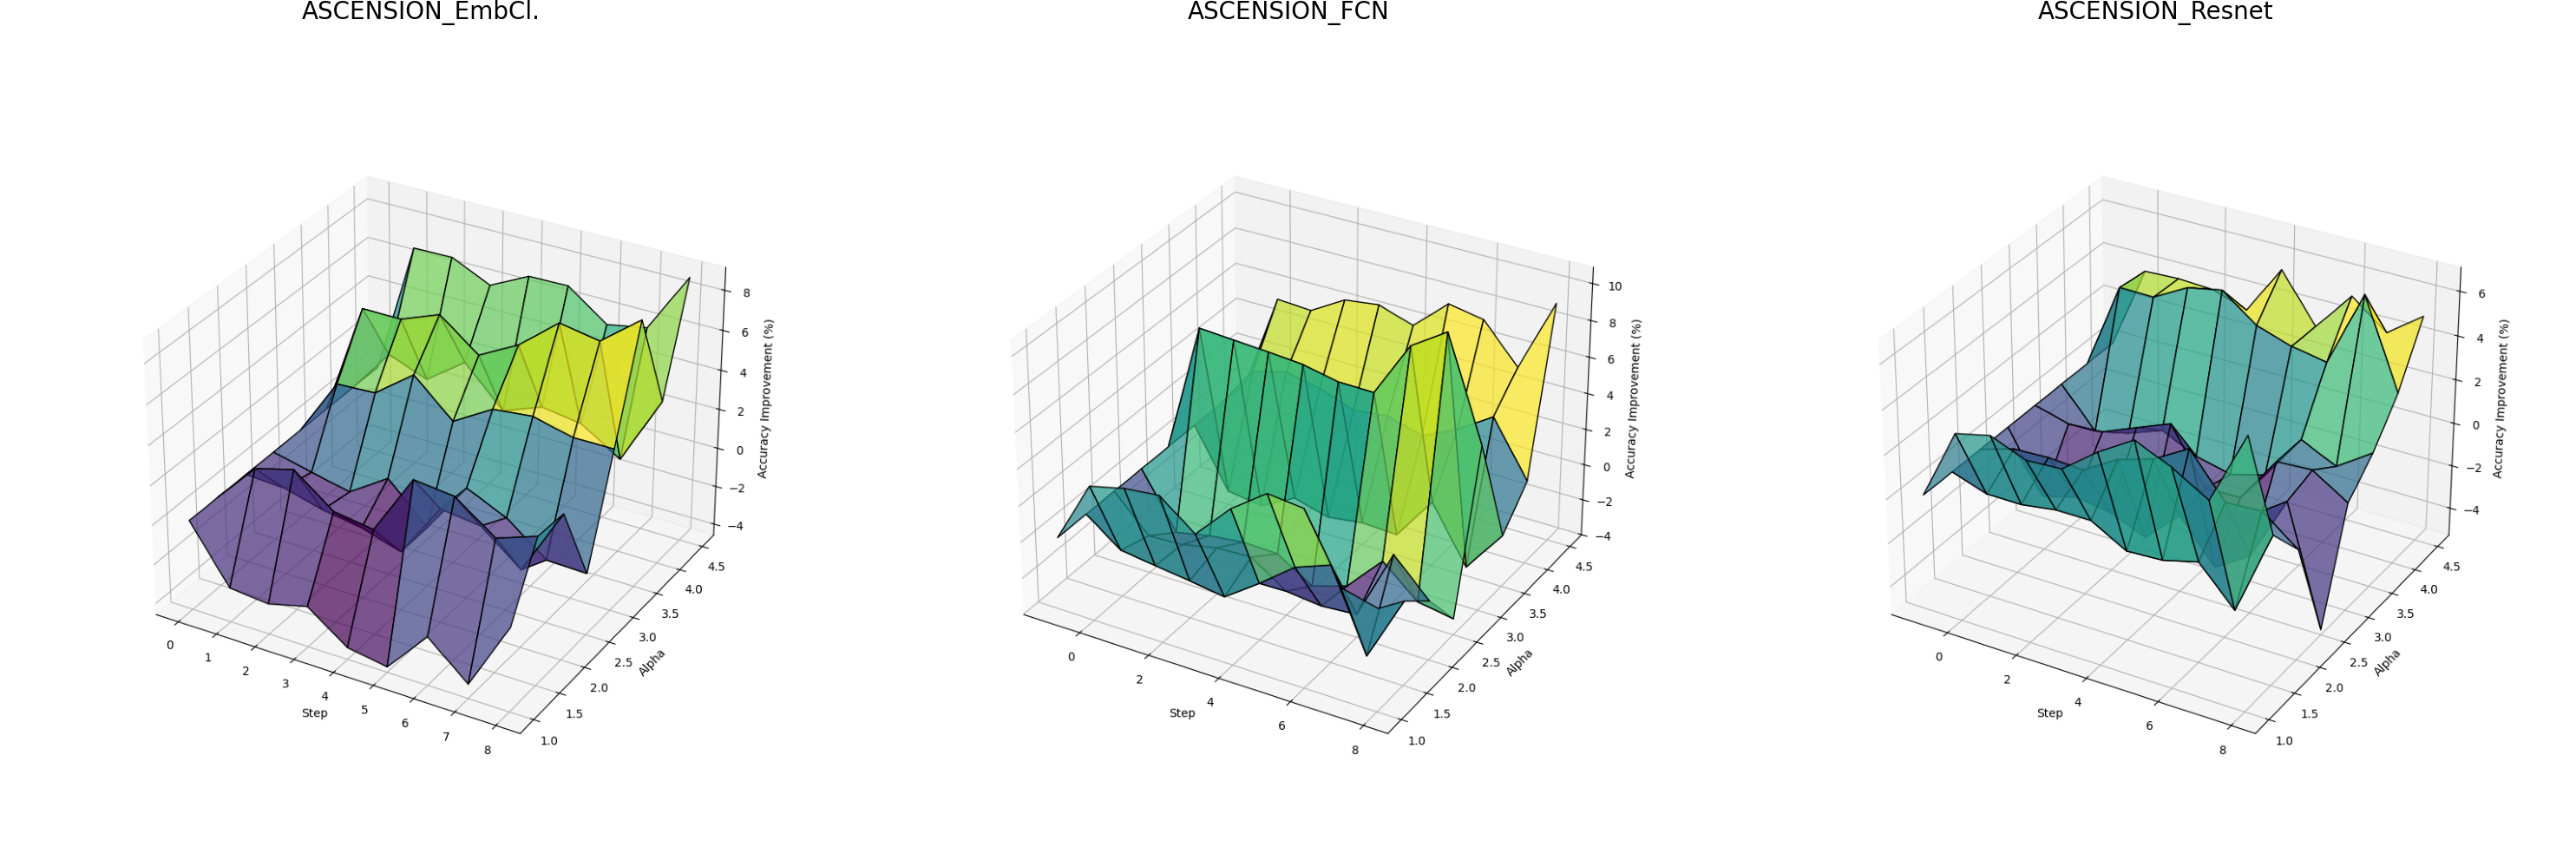
\includegraphics[width=\linewidth,clip=true,trim=0cm 3cm 0cm 5cm]{images/alpha_study_combined_SemgHandMovementCh2.png}
%     \caption{\textbf{Spectrum:} Classifier performance against $\alpha$ and iteration number for \textbf{SemgHandMovementCh2} dataset.}
%     \label{fig:images/alpha_study_SemgHandMovementCh2}
% \end{figure}

% % Device
% \begin{figure}[H]
%     \centering
%       
%     \hspace{1.5cm} ASCENSION$_\text{Emb.}$ \hfill ASCENSION$_\text{FCN-Emb.}$ \hfill ASCENSION$_\text{ResNet-Emb.}$ \hspace{1cm}
%     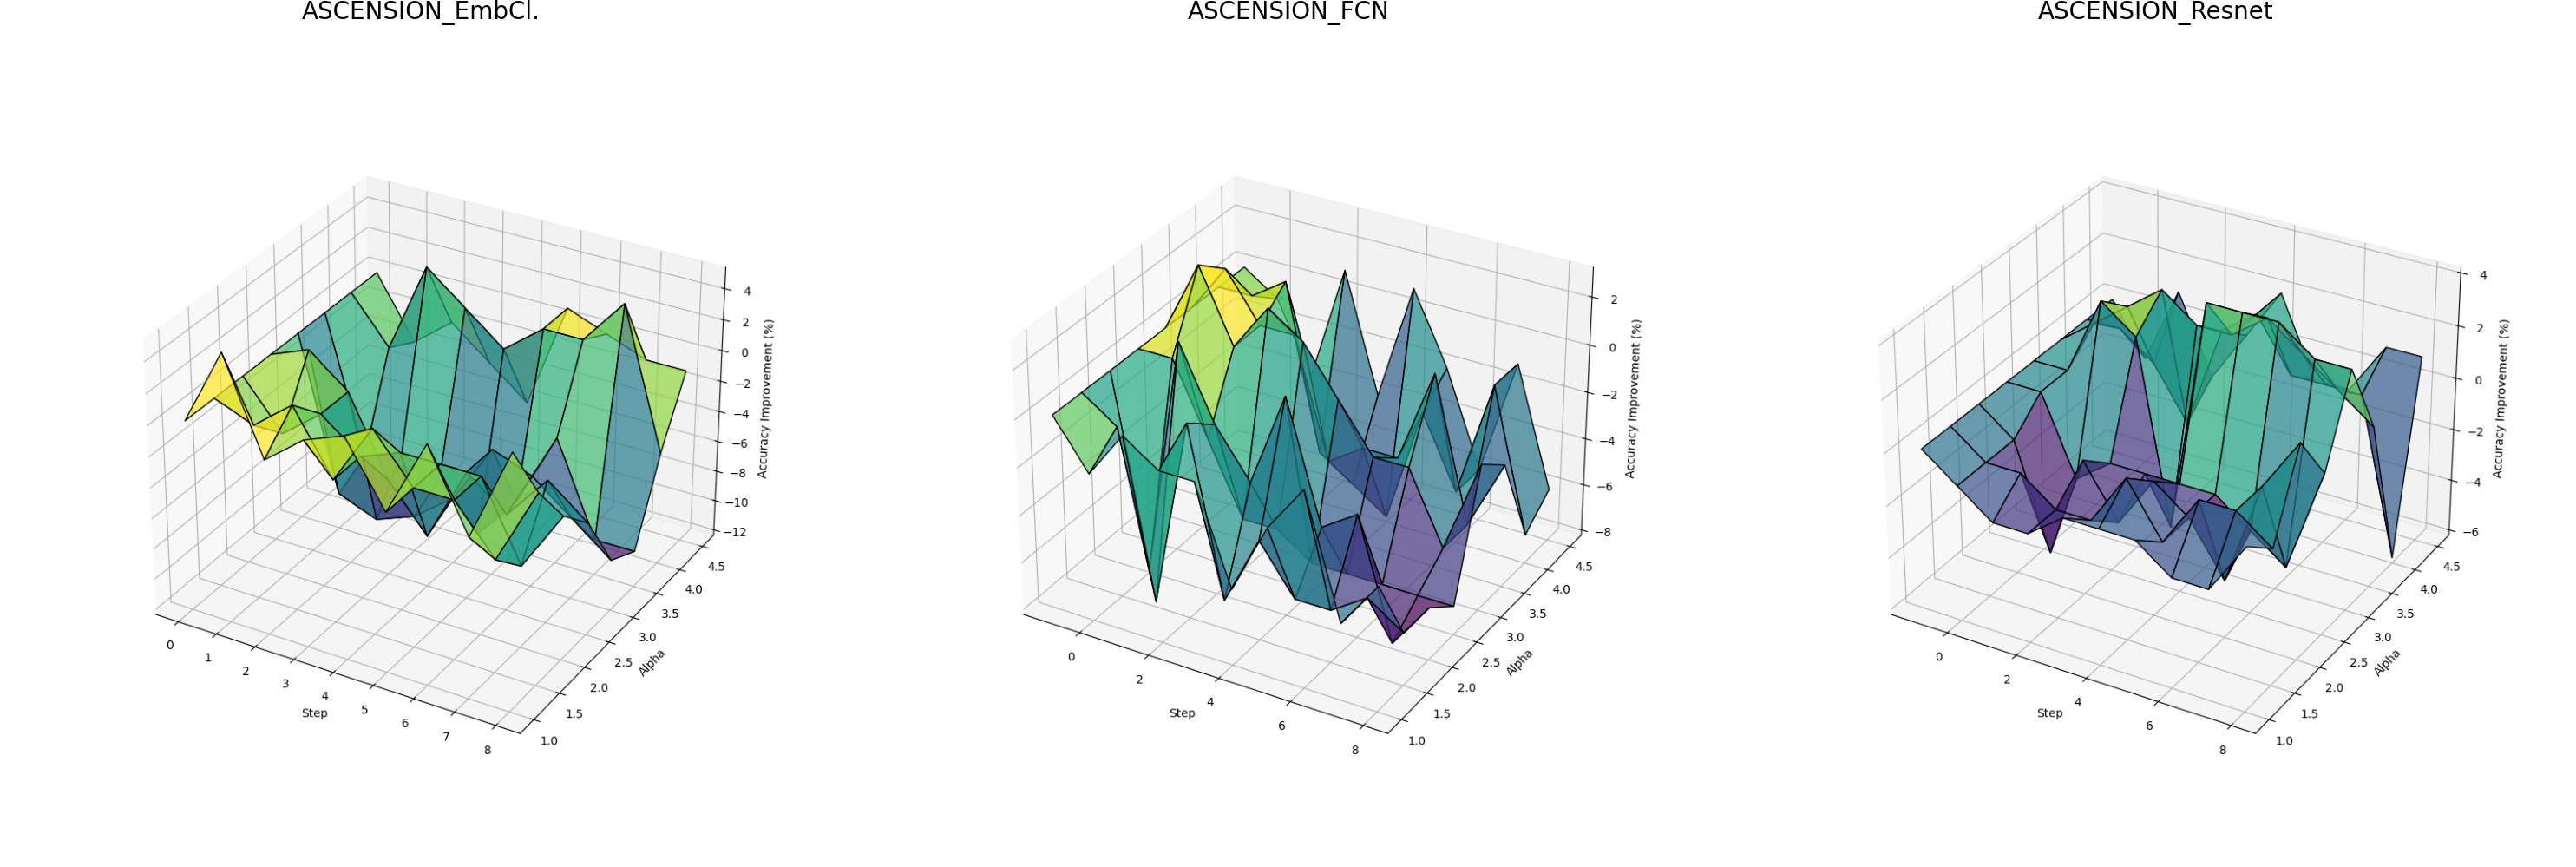
\includegraphics[width=\linewidth,clip=true,trim=0cm 3cm 0cm 5cm]{images/alpha_study_combined_ACSF1.png}
%     \caption{\textbf{Device:} Classifier performance against $\alpha$ and iteration number for \textbf{ACSF1} dataset.}
%     \label{fig:images/alpha_study_ACSF1}
% \end{figure}


\subsection{Clustering loss ablation study}\label{app:HPSA:clusterL}\label{app:loss_weights}
\tablename~\ref{Tab:app:Ablation_clustering_alpha} illustrates the step-wise performance evolution given the clustering loss removal via setting the clustering loss weight parameter $\gamma_3$ to zero. To quantify this evolution, we compute the average step-wise improvement using Equation \eqref{Eq:Delta_Acc_Alpha_Cluster}. Removing the clustering loss results in a performance decrease from $2.1\%$ to $-0.05\%$ with ASCENSION$_{\text{ResNet-Emb}}$, and from $1.2\%$ to $-0.05\%$ with ASCENSION$_{\text{FCN-Emb}}$ (see \tablename~\ref{tab:embedded}).
\begin{equation}\label{Eq:Delta_Acc_Alpha_Cluster}
\overline{Acc}_{\Delta_1 Step} = \frac{1}{n - 1} \sum_{k = 2}^{n} \left( Acc_{Step\_k} - Acc_{Step\_1}\right),
\end{equation}
where $n$ is the total number of augmentation steps, $Acc_{Step\_1}$ is the accuracy at the first augmentation step (taken as the reference), and the sum averages the per-step accuracy delta over subsequent steps $k = 2, \ldots, n$.

%$$\overline{Acc}_{\Delta_1 Step} = \frac{1}{n - 1} \sum_{k = 2}^{n - 1} \left( Acc_{Step\_k}\right) - Acc_{Step\_1} $$,

%where n denotes the total number of adaptation steps and  $Acc_{\text{Step\_k}}$ is the classification accuracy at step k.


% \begin{table*}[p]
% \centering
%  
% \caption{  \red Accuracy gain ($\overline{Acc}_{\Delta_1 Step}$) after first augmentation step per dataset for the $\alpha$-scaling mechanism and clustering loss ablation studies}\label{Table:app:Ablation_clustering}
% \begin{tabular}{@{}ll|ll@{}}
% \toprule
% \# & $\overline{Acc}_{\Delta_1 Step}$ & \# & $\overline{Acc}_{\Delta_1 Step}$ \\
% \midrule
% D1 & -0.01 & D54 & 0.01 \\
% D2 & -0.01 & D55 & -0.02 \\
% D3 & -0.05 & D56 & -0.03 \\
% D4 & 0.03 & D57 & 0.00 \\
% D5 & 0.13 & D58 & 0.01 \\
% D6 & 0.00 & D59 & 0.00 \\
% D7 & -0.02 & D60 & -0.00 \\
% D8 & -0.02 & D61 & 0.01 \\
% D9 & 0.01 & D62 & 0.01 \\
% D10 & 0.00 & D63 & 0.00 \\
% D11 & -0.00 & D64 & -0.00 \\
% D12 & -0.13 & D65 & 0.00 \\
% D13 & 0.02 & D66 & 0.00 \\
% D14 & -0.01 & D67 & -0.02 \\
% D15 & 0.03 & D68 & -0.01 \\
% D16 & 0.00 & D69 & -0.00 \\
% D17 & -0.02 & D70 & -0.01 \\
% D18 & -0.01 & D71 & -0.01 \\
% D19 & -0.00 & D72 & 0.02 \\
% D20 & 0.00 & D73 & 0.01 \\
% D21 & 0.00 & D74 & -0.03 \\
% D22 & -0.01 & D75 & -0.01 \\
% D23 & -0.02 & D76 & 0.00 \\
% D24 & 0.01 & D77 & -0.02 \\
% D25 & -0.00 & D78 & 0.01 \\
% D26 & 0.02 & D79 & 0.01 \\
% D27 & -0.06 & D80 & -0.00 \\
% D28 & -0.01 & D81 & -0.01 \\
% D29 & -0.04 & D82 & -0.01 \\
% D30 & -0.00 & D83 & -0.01 \\
% D31 & -0.01 & D84 & -0.01 \\
% D32 & -0.00 & D85 & -0.02 \\
% D33 & 0.03 & D86 & 0.00 \\
% D34 & -0.02 & D87 & -0.04 \\
% D35 & -0.00 & D88 & 0.02 \\
% D36 & -0.01 & D89 & -0.01 \\
% D37 & 0.00 & D90 & 0.01 \\
% D38 & -0.03 & D91 & -0.01 \\
% D39 & -0.00 & D92 & 0.02 \\
% D40 & -0.01 & D93 & -0.01 \\
% D41 & 0.02 & D94 & -0.00 \\
% D42 & 0.00 & D95 & 0.01 \\
% D43 & -0.02 & D96 & -0.01 \\
% D44 & -0.00 & D97 & -0.00 \\
% D45 & 0.00 & D98 & 0.01 \\
% D46 & 0.00 & D99 & -0.01 \\
% D47 & -0.00 & D100 & -0.02 \\
% D48 & -0.01 & D101 & -0.03 \\
% D49 & -0.04 & D102 & -0.02 \\
% D50 & -0.04 & & \\
% D51 & 0.01 & & \\
% D52 & -0.02 & & \\
% D53 & -0.01 & & \\
% \bottomrule
% \end{tabular}
% \end{table*}












% \subsection{Loss weights' tuning} \label{app:HPSA:lossW}
% \textcolor{red}{TEST In this section, we describe the 22~time series features (Catch22) presented in  and the two additional features (denoted by F23 and F24 below) considered in this study. In this section, we describe the 22~time series features (Catch22) presented, and the two additional features (denoted by F23 and F24 below) considered in this study. TEST}


% Trust Results Analysis
%\input{sections/appendix/trust_analysis}



% ========== Iteration count under a fixed budget (TMLR rebuttal Q3) ==========
% ADDED FOR TMLR (rebuttal Q3)
\subsection{Iteration count under a fixed generation budget}
\label{app:budget-matched}

\tablename s~\ref{Tab:app:bestconfig:resnet}--\ref{Tab:app:bestconfig:moment}
show that in more than half the cases a single iteration already gives
the best result. To separate the effect of the iteration count from the
effect of the total generation budget, we run a controlled experiment
with a fixed generation budget on 10 datasets with ResNet and a single
seed. \tablename~\ref{tab:budget-matched} reports the mean gain of each
configuration.

\begin{table}[H]
\centering
\small
\caption{Mean accuracy gain (accuracy points) under a controlled
generation budget, on 10 datasets with ResNet and a single seed.}
\label{tab:budget-matched}
\begin{tabular}{lccr}
\toprule
\textbf{Configuration} & \textbf{Budget} & \textbf{Iterations} & \textbf{Mean gain} \\
\midrule
Deployed    & $1\times$ & 1 & $+0.12$ \\
Single pass & $4\times$ & 1 & $-0.18$ \\
Spread      & $4\times$ & 4 & $-0.10$ \\
\bottomrule
\end{tabular}
\end{table}

Spreading the same budget over four iterations gives no systematic
advantage, and quadrupling the budget does not improve on the deployed
configuration.


% ========== Feature \& expansion risk analysis (ICML app:) ==========
\section{Feature description \& Class expansion risk analysis}\label{app:feature_risk}

\subsection{Time series features}\label{app:TSF}
We describe hereinafter the 22~TS features (Catch22) presented in \citep{lubba2019catch22}, and the two additional features (denoted by F23 and F24 below) considered in this study.

{ 
\begin{description}
    \item[\textbf{F1}: \texttt{DN\_HistogramMode\_5}] Top z-score range based on the highest count from a 5-bin histogram, representing the most frequent distribution range in the dataset.
    
    \item[\textbf{F2}: \texttt{DN\_HistogramMode\_10}] Similar to DN5, but this considers the top z-score range based on a 10-bin histogram, providing a finer resolution.
    
    \item[\textbf{F3}: \texttt{CO\_f1ecac}] Represents the first 1/e crossing of the autocorrelation function, indicating how quickly the autocorrelation of a time series decays.
    
    \item[\textbf{F4}: \texttt{CO\_FirstMin\_ac}] Identifies the first minimum of the autocorrelation function, which helps analyze the periodicity of the time series.
    
    \item[\textbf{F5}: \texttt{CO\_HistogramAMI\_even\_2\_5}] Automutual information for $m = 2$ and $\tau = 5$, capturing the dependency between data points across time.
    
    \item[\textbf{F6}: \texttt{CO\_trev\_1\_num}] This statistic measures time-reversibility, focusing on the differences between successive points in the time series raised to the third power.
    
    \item[\textbf{F7}: \texttt{MD\_hrv\_classic\_pnn40}] Proportion of successive differences in time series values that exceed 0.04 of the standard deviation, indicating rapid fluctuations.
    
    \item[\textbf{F8}: \texttt{SB\_BinaryStats\_mean\_longstretch1}] The longest period where values stay consecutively above the mean, representing persistent trends in the data.
    
    \item[\textbf{F9}: \texttt{SB\_TransitionMatrix\_3ac\_sumdiagcov}] Trace of the covariance of the transition matrix between symbols in a 3-letter alphabet, used to assess transitions in symbolized data.
    
    \item[\textbf{F10}: \texttt{PD\_PeriodicityWang\_th0\_01}] A periodicity measure, indicating how regularly patterns repeat within the time series.
    
    \item[\textbf{F11}: \texttt{CO\_Embed2\_Dist\_tau\_d\_expfit\_meandiff}] Exponential fit to the differences in distances between successive points in a 2-dimensional embedding space, revealing structural relationships.
    
    \item[\textbf{F12}: \texttt{IN\_AutoMutlInfoStats\_40\_gaussian\_fmmi}] First minimum of the automutual information function, which gives insight into the periodicity and structure of the time series.
    
    \item[\textbf{F13}: \texttt{FC\_LocalSimple\_mean1\_tauresrat}] Measures the change in correlation length after iteratively differencing the time series, providing insights into the stationarity of the data.
    
    \item[\textbf{F14}: \texttt{DN\_OutlierInclude\_p\_001\_mdrmd}] Measures the time intervals between successive extreme events occurring above the mean, indicating patterns of high values.
    
    \item[\textbf{F15}: \texttt{DN\_OutlierInclude\_n\_001\_mdrmd}] Similar to DNOp but for extreme events occurring below the mean, highlighting the time intervals between low-value outliers.
    
    \item[\textbf{F16}: \texttt{SP\_Summaries\_welch\_rect\_area\_5\_1}] This computes the total power in the lowest fifth of the frequencies from a Fourier power spectrum, reflecting long-term trends.
    
    \item[\textbf{F17}: \texttt{SB\_BinaryStats\_diff\_longstretch0}] The longest period of successive decreases in the time series, capturing prolonged declining trends.
    
    \item[\textbf{F18}: \texttt{SB\_MotifThree\_quantile\_hh}] Shannon entropy of successive symbol pairs in a 3-letter quantile symbolization, quantifying the complexity of transitions between motifs.
    
    \item[\textbf{F19}: \texttt{SC\_FluctAnal\_2\_rsrangefit\_50\_1}] Proportion of slower timescale fluctuations that scale with rescaled range fits, indicating long-term memory in the data.
    
    \item[\textbf{F20}: \texttt{SC\_FluctAnal\_2\_dfa\_50\_1\_2\_logi\_prop}] Proportion of slower timescale fluctuations that scale with detrended fluctuation analysis (DFA) under 50% sampling.
    
    \item[\textbf{F21}: \texttt{SP\_Summaries\_welch\_rect\_centroid}] The centroid of the Fourier power spectrum, which offers a measure of the central frequency or the dominant pattern in the time series.
    
    \item[\textbf{F22}: \texttt{FC\_LocalSimple\_mean3\_stderr}] Calculates the mean error from a rolling 3-sample mean forecast, capturing the volatility of short-term predictions.
    
    \item[\textbf{F23}: \texttt{Train\_Test\_Ratio}] The ratio of training data to test data in the dataset.
    \item[\textbf{F24}: \texttt{Discrepancy\_in\_Distance}] To estimate the discrepancy in distance between the training and testing set distributions, as defined in Appendix~\ref{app:discrepancy:form}.
    \label{app:desc:tsf}
\end{description}
}




% -----------------------------------------------------------------
% NOTE (commented out 2026-05-11): App. K.2 (Extended analysis of
% class assignment confidence) was orphaned -- no \ref pointed at it
% from outside the subsection, and its conclusion ('no clear linear or
% polynomial correlation between confidence and accuracy delta') is
% weakly informative. Pairs with the already-commented App. F
% (Empirical acceptance rate). Body kept here for potential revival
% during TMLR rebuttal.
% -----------------------------------------------------------------
% \subsection{Extended analysis of the class assignment confidence}\label{app:TrustAnalysis}
% Figures~\ref{fig:trust_perf_resnet} and \ref{fig:trust_perf_fcn} visualize the relationship between the confidence of synthetic sample class assignments (i.e., confidence that a generated sample is correctly labeled) and the resulting change in classifier accuracy using ASCENSION with ResNet and FCN as external classifiers. Confidence is plotted on the $y$-axis and accuracy delta on the $x$-axis. For both classifiers the relationship appears complex. A weak positive trend may exist, but there is no clear linear or polynomial correlation.
% 
% To deepen the analysis, Figures~\ref{fig:trust_perf_resnet_clustering} and \ref{fig:trust_perf_fcn_clustering} apply \texttt{DBSCAN} clustering to uncover patterns. Two main clusters emerge: one (orange / cluster1) suggests that confidence remains largely constant regardless of performance, while the second (blue / cluster2) shows no clear trend. These clusters likely reflect differences in the intrinsic features of the time series datasets. To investigate this, we assess the influence of the 24~dataset features (F1-F24, see Appendix~\ref{app:desc:tsf}) with ASCENSION (ResNet) on confidence scores using a shallow random forest with many estimators, as in Section~\ref{sec:analysis:features}. Feature importance results in Figure~\ref{fig:trust_feature_importance} highlight seven dominant features (importance $\geq 0.6$), supporting the hypothesis that certain dataset characteristics affect confidence levels in the expansion mechanism.
% 
% 
% \begin{figure*}[h]
%     \centering  
%     \psset{xunit=1mm,yunit=1mm,runit=1mm}
% 
% 
%     
% \scalebox{1.0}{
% \begin{pspicture}(0,0)(140,31.5)
%     
%     \put(-5.5,-2){% GNUPLOT: LaTeX picture with Postscript
\begingroup
  \makeatletter
  \providecommand\color[2][]{%
    \GenericError{(gnuplot) \space\space\space\@spaces}{%
      Package color not loaded in conjunction with
      terminal option `colourtext'%
    }{See the gnuplot documentation for explanation.%
    }{Either use 'blacktext' in gnuplot or load the package
      color.sty in LaTeX.}%
    \renewcommand\color[2][]{}%
  }%
  \providecommand\includegraphics[2][]{%
    \GenericError{(gnuplot) \space\space\space\@spaces}{%
      Package graphicx or graphics not loaded%
    }{See the gnuplot documentation for explanation.%
    }{The gnuplot epslatex terminal needs graphicx.sty or graphics.sty.}%
    \renewcommand\includegraphics[2][]{}%
  }%
  \providecommand\rotatebox[2]{#2}%
  \@ifundefined{ifGPcolor}{%
    \newif\ifGPcolor
    \GPcolortrue
  }{}%
  \@ifundefined{ifGPblacktext}{%
    \newif\ifGPblacktext
    \GPblacktexttrue
  }{}%
  % define a \g@addto@macro without @ in the name:
  \let\gplgaddtomacro\g@addto@macro
  % define empty templates for all commands taking text:
  \gdef\gplbacktext{}%
  \gdef\gplfronttext{}%
  \makeatother
  \ifGPblacktext
    % no textcolor at all
    \def\colorrgb#1{}%
    \def\colorgray#1{}%
  \else
    % gray or color?
    \ifGPcolor
      \def\colorrgb#1{\color[rgb]{#1}}%
      \def\colorgray#1{\color[gray]{#1}}%
      \expandafter\def\csname LTw\endcsname{\color{white}}%
      \expandafter\def\csname LTb\endcsname{\color{black}}%
      \expandafter\def\csname LTa\endcsname{\color{black}}%
      \expandafter\def\csname LT0\endcsname{\color[rgb]{1,0,0}}%
      \expandafter\def\csname LT1\endcsname{\color[rgb]{0,1,0}}%
      \expandafter\def\csname LT2\endcsname{\color[rgb]{0,0,1}}%
      \expandafter\def\csname LT3\endcsname{\color[rgb]{1,0,1}}%
      \expandafter\def\csname LT4\endcsname{\color[rgb]{0,1,1}}%
      \expandafter\def\csname LT5\endcsname{\color[rgb]{1,1,0}}%
      \expandafter\def\csname LT6\endcsname{\color[rgb]{0,0,0}}%
      \expandafter\def\csname LT7\endcsname{\color[rgb]{1,0.3,0}}%
      \expandafter\def\csname LT8\endcsname{\color[rgb]{0.5,0.5,0.5}}%
    \else
      % gray
      \def\colorrgb#1{\color{black}}%
      \def\colorgray#1{\color[gray]{#1}}%
      \expandafter\def\csname LTw\endcsname{\color{white}}%
      \expandafter\def\csname LTb\endcsname{\color{black}}%
      \expandafter\def\csname LTa\endcsname{\color{black}}%
      \expandafter\def\csname LT0\endcsname{\color{black}}%
      \expandafter\def\csname LT1\endcsname{\color{black}}%
      \expandafter\def\csname LT2\endcsname{\color{black}}%
      \expandafter\def\csname LT3\endcsname{\color{black}}%
      \expandafter\def\csname LT4\endcsname{\color{black}}%
      \expandafter\def\csname LT5\endcsname{\color{black}}%
      \expandafter\def\csname LT6\endcsname{\color{black}}%
      \expandafter\def\csname LT7\endcsname{\color{black}}%
      \expandafter\def\csname LT8\endcsname{\color{black}}%
    \fi
  \fi
    \setlength{\unitlength}{0.0500bp}%
    \ifx\gptboxheight\undefined%
      \newlength{\gptboxheight}%
      \newlength{\gptboxwidth}%
      \newsavebox{\gptboxtext}%
    \fi%
    \setlength{\fboxrule}{0.5pt}%
    \setlength{\fboxsep}{1pt}%
    \definecolor{tbcol}{rgb}{1,1,1}%
\begin{picture}(8640.00,2016.00)%
    \gplgaddtomacro\gplbacktext{%
      \csname LTb\endcsname%%
      \put(800,711){\makebox(0,0)[r]{\strut{}\footnotesize$0.02$}}%
      \csname LTb\endcsname%%
      \put(800,982){\makebox(0,0)[r]{\strut{}\footnotesize$0.04$}}%

      \put(350,1050){\makebox(0,0)[r]{\strut{}\footnotesize\rotatebox{90}{Importance}}}%
      \csname LTb\endcsname%%
      \put(800,1254){\makebox(0,0)[r]{\strut{}\footnotesize$0.06$}}%
      \csname LTb\endcsname%%
      \put(800,1525){\makebox(0,0)[r]{\strut{}\footnotesize$0.08$}}%
      \put(1153,220){\makebox(0,0){\strut{}\scriptsize F1}}%
      \put(1449,220){\makebox(0,0){\strut{}\scriptsize F2}}%
      \put(1744,220){\makebox(0,0){\strut{}\scriptsize F3}}%
      \put(2039,220){\makebox(0,0){\strut{}\scriptsize F4}}%
      \put(2335,220){\makebox(0,0){\strut{}\scriptsize F5}}%
      \put(2630,220){\makebox(0,0){\strut{}\scriptsize F6}}%
      \put(2926,220){\makebox(0,0){\strut{}\scriptsize F7}}%
      \put(3221,220){\makebox(0,0){\strut{}\scriptsize F8}}%
      \put(3516,220){\makebox(0,0){\strut{}\scriptsize F9}}%
      \put(3812,220){\makebox(0,0){\strut{}\scriptsize F10}}%
      \put(4107,220){\makebox(0,0){\strut{}\scriptsize F11}}%
      \put(4402,220){\makebox(0,0){\strut{}\scriptsize F12}}%
      \put(4698,220){\makebox(0,0){\strut{}\scriptsize F13}}%
      \put(4993,220){\makebox(0,0){\strut{}\scriptsize F14}}%
      \put(5288,220){\makebox(0,0){\strut{}\scriptsize F15}}%
      \put(5584,220){\makebox(0,0){\strut{}\scriptsize F16}}%
      \put(5879,220){\makebox(0,0){\strut{}\scriptsize F17}}%
      \put(6174,220){\makebox(0,0){\strut{}\scriptsize F18}}%
      \put(6470,220){\makebox(0,0){\strut{}\scriptsize F19}}%
      \put(6765,220){\makebox(0,0){\strut{}\scriptsize F20}}%
      \put(7061,220){\makebox(0,0){\strut{}\scriptsize F21}}%
      \put(7356,220){\makebox(0,0){\strut{}\scriptsize F22}}%
      \put(7651,220){\makebox(0,0){\strut{}\scriptsize F23}}%
      \put(7947,220){\makebox(0,0){\strut{}\scriptsize F24}}%
    }%
    \gplgaddtomacro\gplfronttext{%
    }%
    \gplbacktext
    \put(0,0){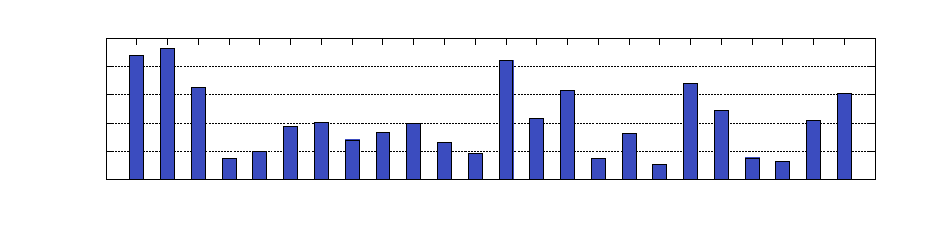
\includegraphics[width={432.00bp},height={100.80bp}]{images/FI_risk_formatted}}%
    \gplfronttext
  \end{picture}%
\endgroup
}
% 
%     \end{pspicture}
%     }
%     \caption{\textbf{Feature importance in regards to confidence:} Overview of the impact of every dataset feature (F1-F24, see Appendix~\ref{app:desc:tsf}) on the mean confidence over the augmentation steps.}.
%     \label{fig:trust_feature_importance}
% \end{figure*}
% 
% 
% \begin{figure*}[t]
% \scalebox{1}{
% \centering
% 
% --- Row 1 ---
% \begin{subfigure}[t]{0.49\linewidth}
%   \centering
%   \psset{xunit=1mm,yunit=1mm,runit=1mm}
%   \begin{pspicture}(0,0)(65,60)
%     \put(1,5){
%       \put(3,3){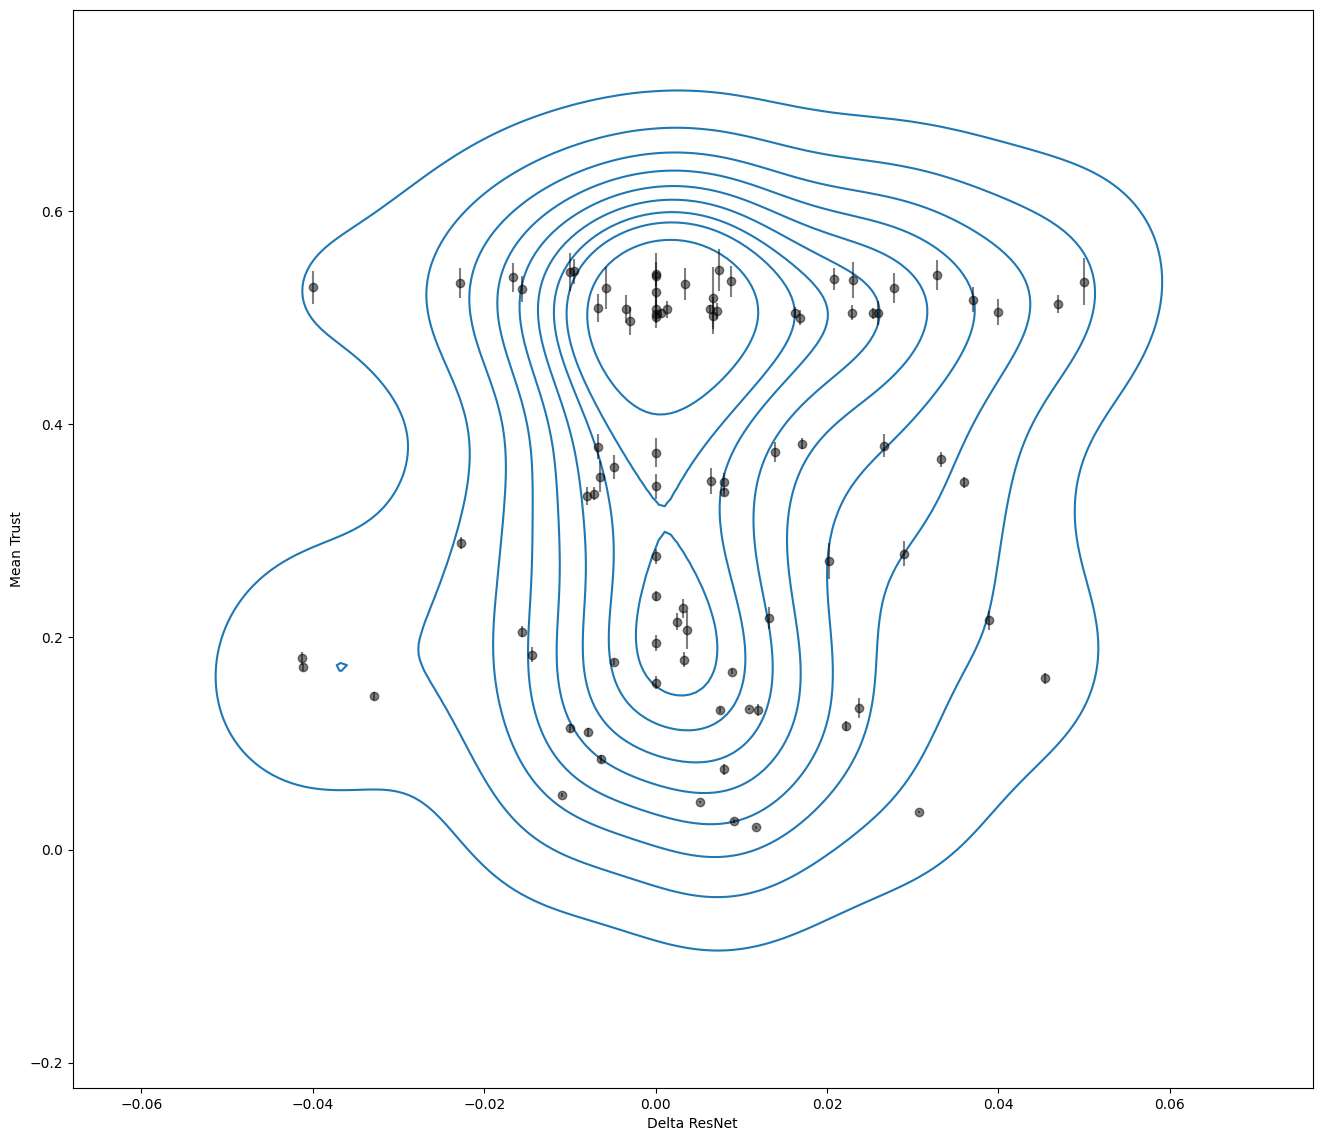
\includegraphics[width=62mm,clip=true,trim=1.7cm 1.2cm .2cm .2cm]{images/trust_perf_resnet.png}}
% 
%       \put(-4,22){\rotatebox{90}{\footnotesize Mean confidence}}
%       \put(-.5,0){
%         \put(0,46){\footnotesize 0.6}
%         \put(0,35.5){\footnotesize 0.4}
%         \put(0,25){\footnotesize 0.2}
%         \put(0,14.5){\footnotesize 0.0}
%         \put(0,4){\footnotesize -0.2}
%       }
% 
%       \put(27,-4){\footnotesize Final delta in accuracy}
%       \put(-.75,0){
%         \put(56.7,0){\footnotesize 0.06}
%         \put(48,0){\footnotesize 0.04}
%         \put(39.5,0){\footnotesize 0.02}
%         \put(31.5,0){\footnotesize 0.00}
%         \put(21.9,0){\footnotesize -0.02}
%         \put(13.7,0){\footnotesize -0.04}
%         \put(5.5,0){\footnotesize -0.06}
%       }
%     }
%   \end{pspicture}
%   \caption{Confidence vs. Performance (ResNet)}
%   \label{fig:trust_perf_resnet}
% \end{subfigure}
% \hfill
% \begin{subfigure}[t]{0.49\linewidth}
%   \centering
%   \psset{xunit=1mm,yunit=1mm,runit=1mm}
%   \begin{pspicture}(0,0)(65,63)
%     \put(1,5){
%       \put(3,3){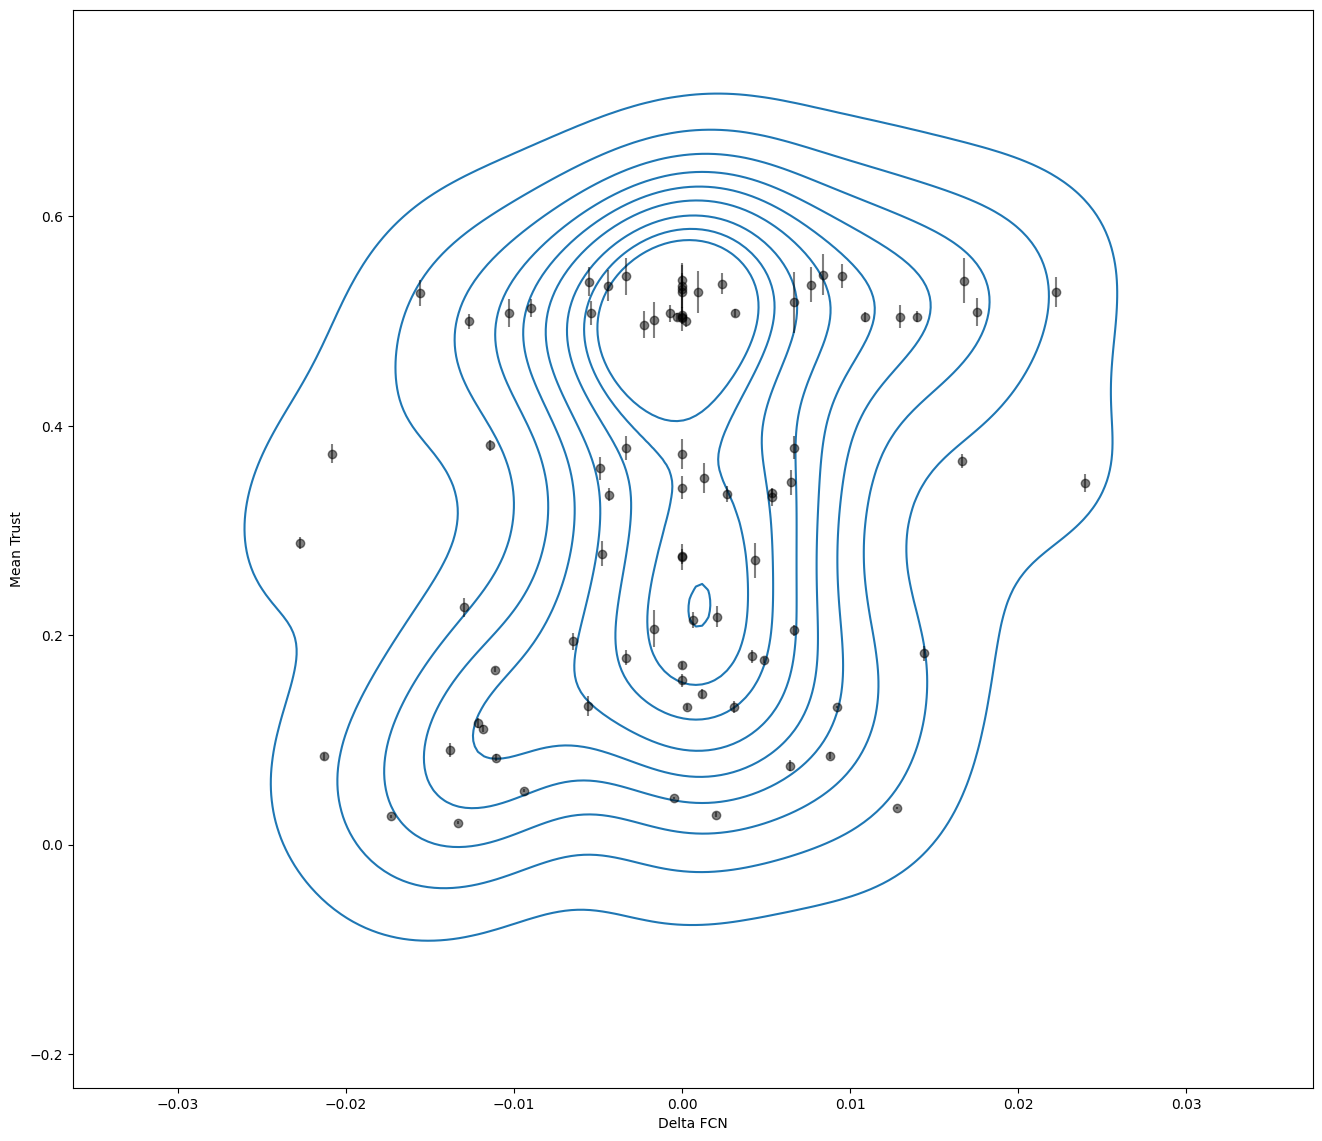
\includegraphics[width=62mm,clip=true,trim=1.7cm 1.2cm .2cm .2cm]{images/trust_perf_fcn.png}}
% 
%       \put(-4,22){\rotatebox{90}{\footnotesize Mean confidence}}
%       \put(-.5,0){
%         \put(0,46){\footnotesize 0.6}
%         \put(0,35.5){\footnotesize 0.4}
%         \put(0,25){\footnotesize 0.2}
%         \put(0,14.5){\footnotesize 0.0}
%         \put(0,4){\footnotesize -0.2}
%       }
% 
%       \put(27,-4){\footnotesize Final delta in accuracy}
%       \put(-.75,0){
%         \put(56.7,0){\footnotesize 0.06}
%         \put(48,0){\footnotesize 0.04}
%         \put(39.5,0){\footnotesize 0.02}
%         \put(31.5,0){\footnotesize 0.00}
%         \put(21.9,0){\footnotesize -0.02}
%         \put(13.7,0){\footnotesize -0.04}
%         \put(5.5,0){\footnotesize -0.06}
%       }
%     }
%   \end{pspicture}
%   \caption{Confidence vs. Performance (FCN)}
%   \label{fig:trust_perf_fcn}
% \end{subfigure}
% }
% 
% \vspace{2mm}
% 
% \scalebox{1}{
% --- Row 2 ---
% \begin{subfigure}[t]{0.49\linewidth}
%   \centering
%   \psset{xunit=1mm,yunit=1mm,runit=1mm}
%   \begin{pspicture}(0,0)(65,63)
%     \put(0,5){
%       \put(3,3){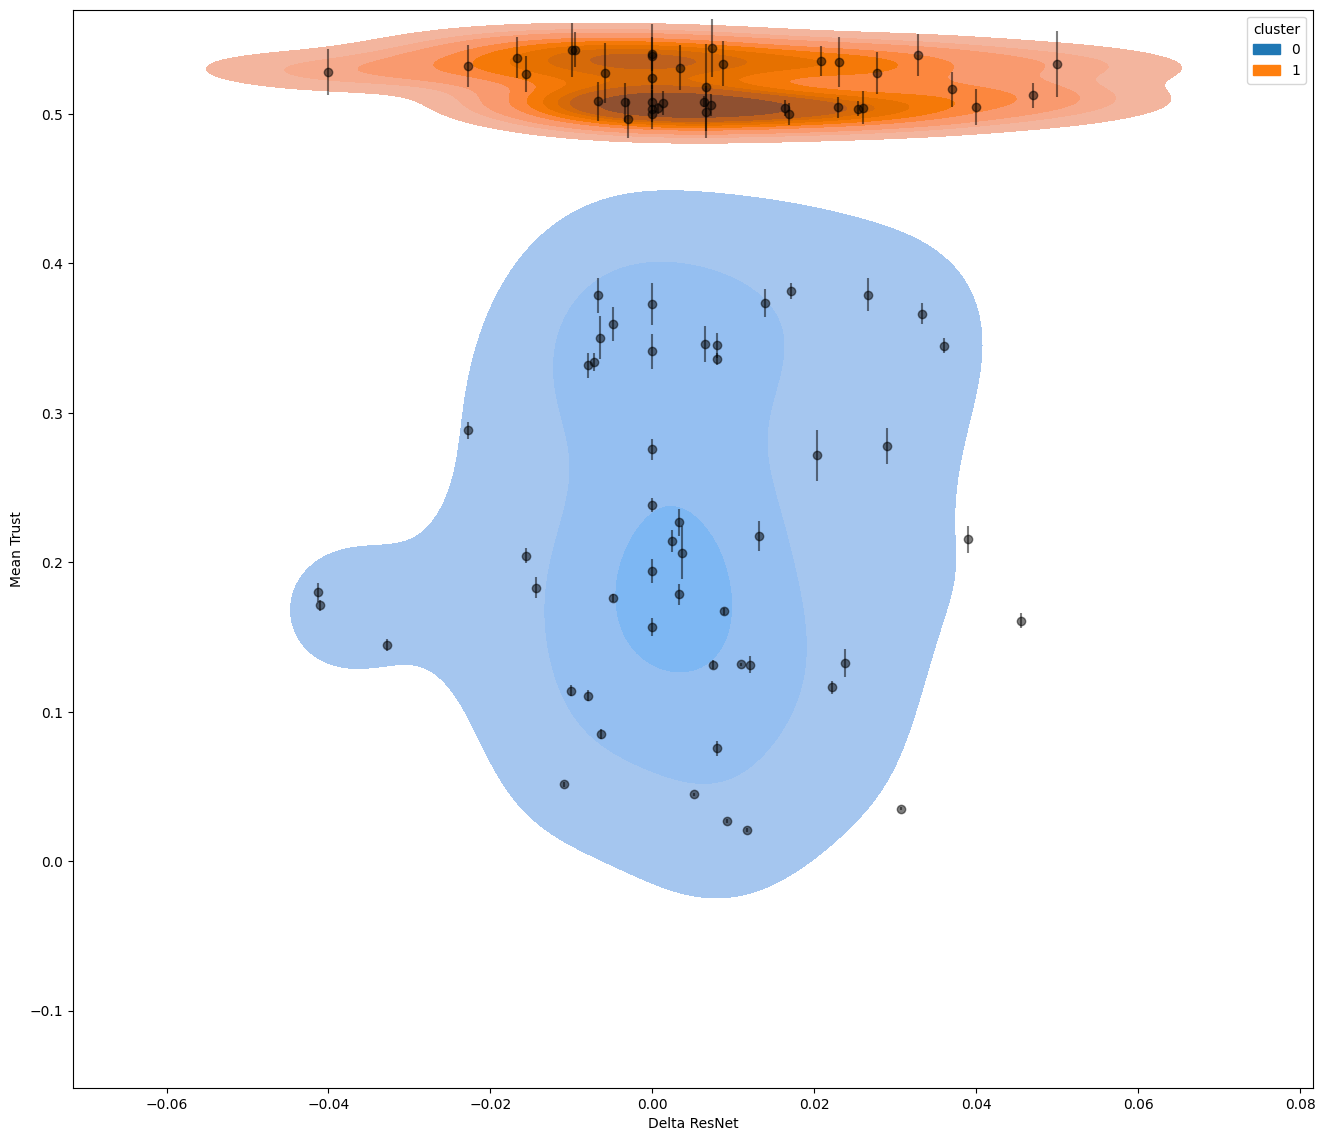
\includegraphics[width=62mm,clip=true,trim=1.7cm 1.2cm .2cm .2cm]{images/trust_perf_resnet_clustering.png}}
% 
%       \put(-4,22){\rotatebox{90}{\footnotesize Mean confidence}}
%       \put(-.5,0){
%         \put(0,51){\footnotesize 0.5}
%         \put(0,43.5){\footnotesize 0.4}
%         \put(0,36){\footnotesize 0.3}
%         \put(0,28.5){\footnotesize 0.2}
%         \put(0,21.2){\footnotesize 0.1}
%         \put(0,14){\footnotesize 0.0}
%         \put(0,6.5){\footnotesize -0.1}
%       }
% 
%       \put(27,-4){\footnotesize Final delta in accuracy}
%       \put(0,0){
%         \put(54.7,0){\footnotesize 0.06}
%         \put(46.5,0){\footnotesize 0.04}
%         \put(38.3,0){\footnotesize 0.02}
%         \put(30.1,0){\footnotesize 0.00}
%         \put(21.9,0){\footnotesize -0.02}
%         \put(13.7,0){\footnotesize -0.04}
%         \put(5.5,0){\footnotesize -0.06}
%       }
%     }
%   \end{pspicture}
%   \caption{Confidence vs. Perf. (ResNet) using \texttt{DBSCAN}}
%   \label{fig:trust_perf_resnet_clustering}
% \end{subfigure}
% \hfill
% \begin{subfigure}[t]{0.49\linewidth}
%   \centering
%   \psset{xunit=1mm,yunit=1mm,runit=1mm}
%   \begin{pspicture}(0,0)(65,60)
%     \put(2,5){
%       \put(3,3){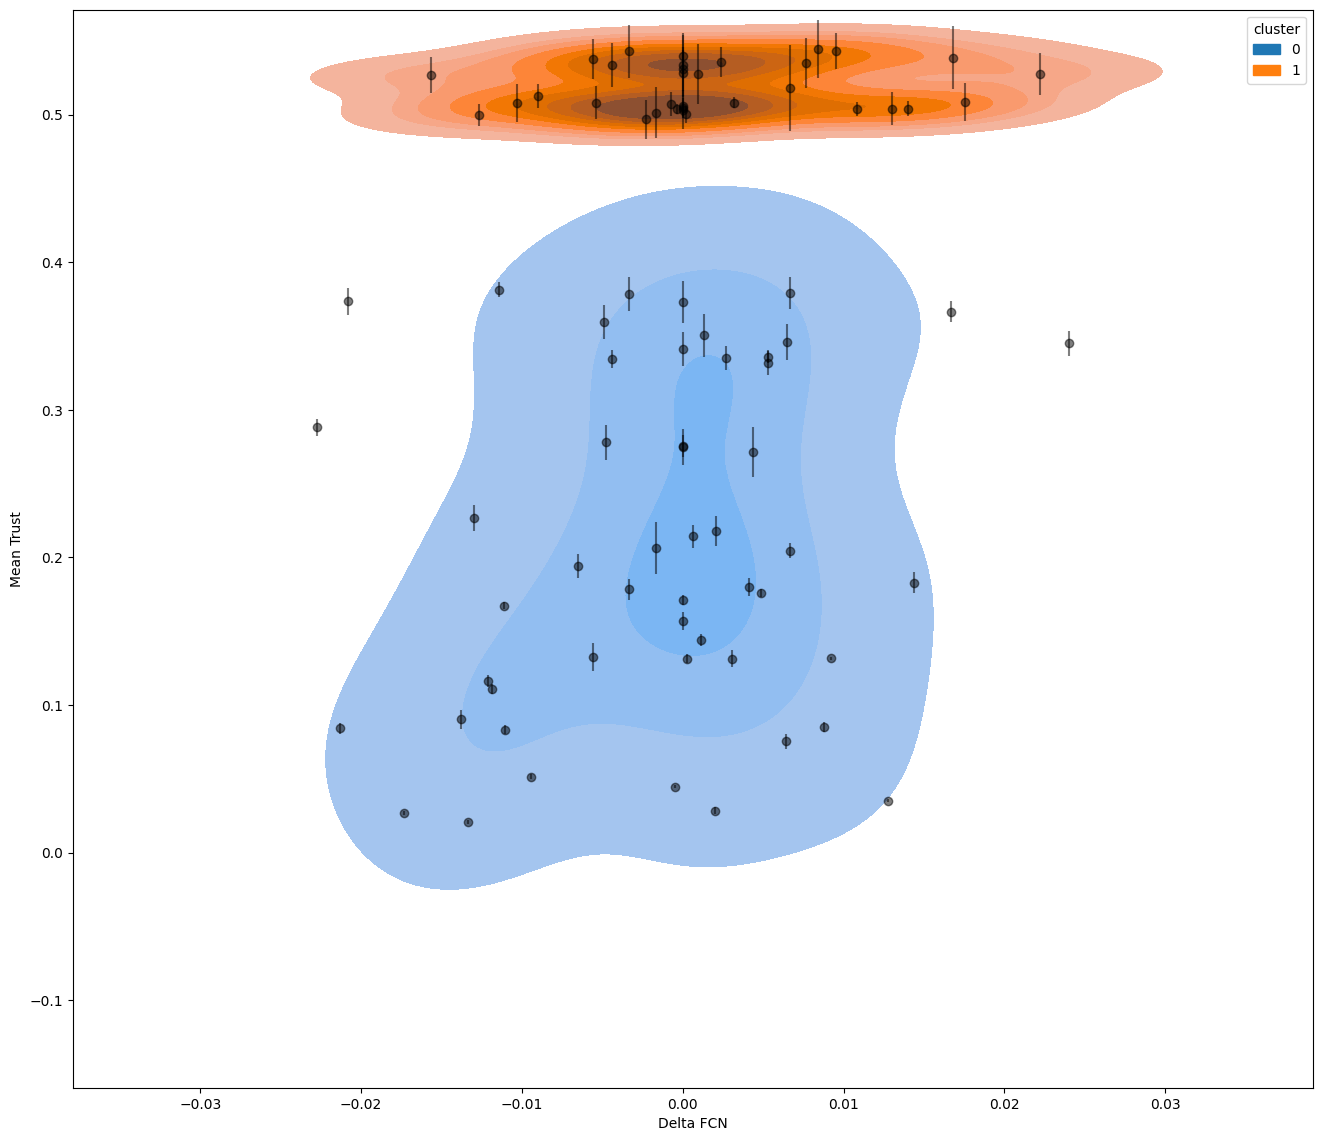
\includegraphics[width=62mm,clip=true,trim=1.7cm 1.2cm .2cm .2cm]{images/trust_perf_fcn_clustering.png}}
% 
%       \put(-.5,0){
%         \put(0,51){\footnotesize 0.5}
%         \put(0,43.5){\footnotesize 0.4}
%         \put(0,36){\footnotesize 0.3}
%         \put(0,28.5){\footnotesize 0.2}
%         \put(0,21.2){\footnotesize 0.1}
%         \put(0,14){\footnotesize 0.0}
%         \put(0,7){\footnotesize -0.1}
%       }
% 
%       \put(27,-4){\footnotesize Final delta in accuracy}
%       \put(0,0){
%         \put(54.7,0){\footnotesize 0.06}
%         \put(46.5,0){\footnotesize 0.04}
%         \put(38.3,0){\footnotesize 0.02}
%         \put(30.1,0){\footnotesize 0.00}
%         \put(21.9,0){\footnotesize -0.02}
%         \put(13.7,0){\footnotesize -0.04}
%         \put(5.5,0){\footnotesize -0.06}
%       }
%     }
%   \end{pspicture}
%   \caption{Confidence vs. Perf. (FCN) using \texttt{DBSCAN}}
%   \label{fig:trust_perf_fcn_clustering}
% \end{subfigure}
% }
% \caption{Confidence vs. delta in accuracy over augmentation steps using DBSCAN}
% \label{Fig:Trust_confidence}
% \end{figure*}
% 
% 
% Figure~\ref{fig:trust_perf_fcn_clustering} and \ref{fig:trust_perf_resnet_clustering} reveal the emergence of two primary clusters. As discussed earlier, these clusters likely reflect variations in the initial augmentation conditions: the specific dataset and its inherent characteristics.
% 
% %All the figures in this section have been computed after removing outlier data samples. All four 
% 
% Both Figures~\ref{fig:trust_perf_fcn} and \ref{fig:trust_perf_resnet} show a complex relationship between confidence and performance. A slight positive correlation appears to be present, however it is clear that no linear or polynomial relationship exists between the two.
% 
% % From the previous analysis, we perform a clustering using \verb|DBSCAN| to extract patterns. Figures~\ref{fig:trust_perf_fcn_clustering} and \ref{fig:trust_perf_resnet_clustering} reveal two main clusters. As mentioned previously, we infer that these clusters may depend on the initial conditions of the augmentation, that is to say, the dataset and its characteristics.
% Based on the previous analysis, we apply \verb|DBSCAN| clustering to identify underlying patterns. Figure~\ref{fig:trust_perf_fcn_clustering} and \ref{fig:trust_perf_resnet_clustering} reveal the emergence of two primary clusters. As discussed earlier, these clusters likely reflect variations in the initial augmentation conditions: the specific dataset and its inherent characteristics.
% 
% Feature importance plot
% \begin{figure*}[h]
%     \centering
%     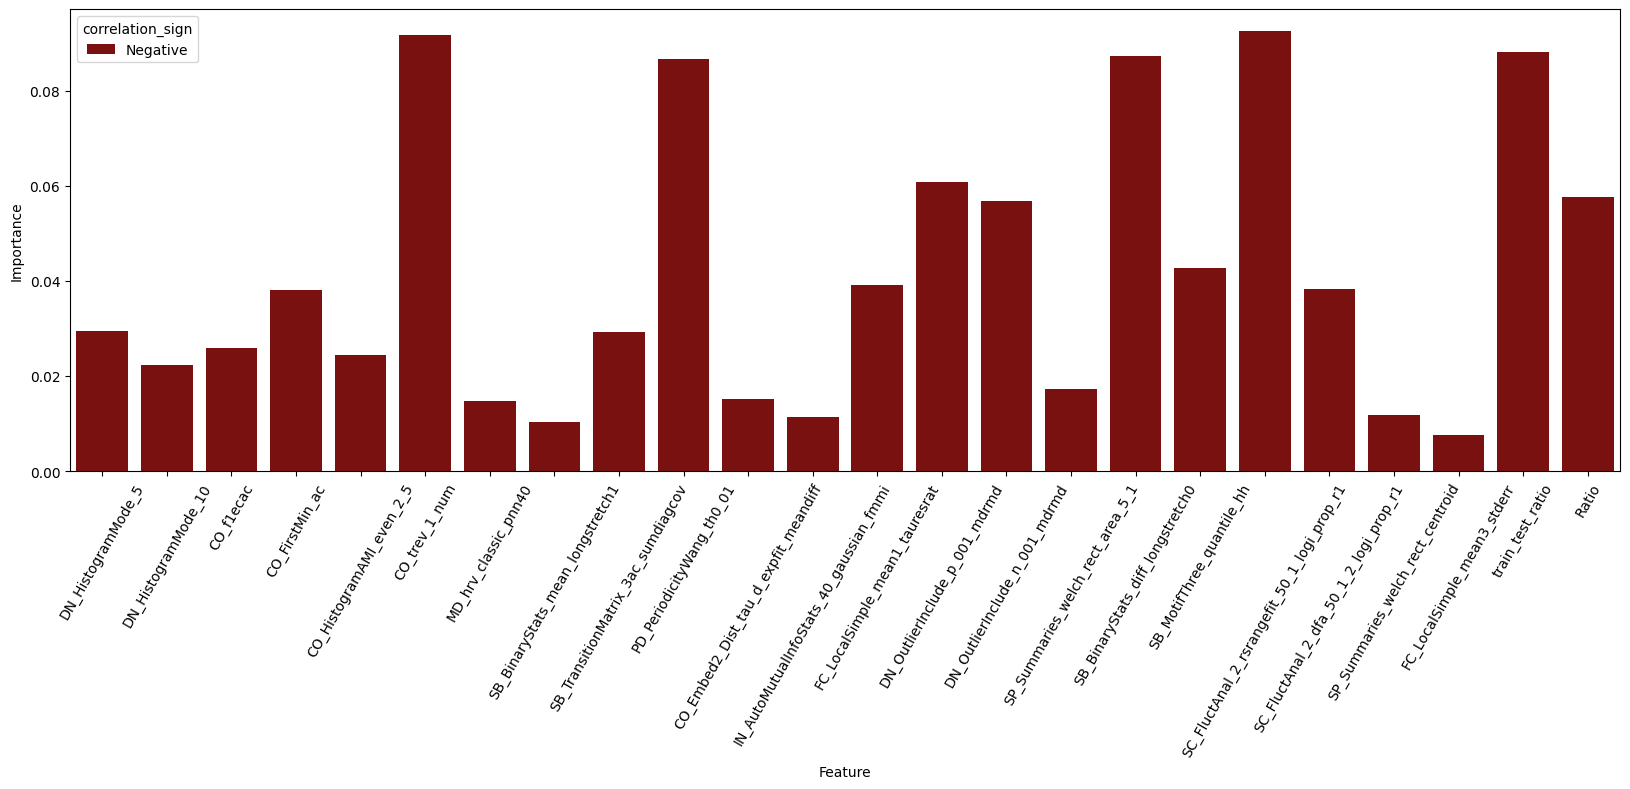
\includegraphics[width=\linewidth,clip=true,trim=0cm 0cm 0cm 0cm]{images/feature_importances_trust.png}
%     \caption{\textbf{Feature importance in regards to confidence:} Overview of the impact of every dataset feature on the mean confidence over the augmentation steps. The red color denotes the negative correlation these features hold with confidence.}.
%     \label{fig:trust_feature_importance}
% \end{figure*}
% 
% 
%\textcolor{red}{(The full tables of results are available in the supplementary materials in csv and json format.) DO WE DO THAT ?}
% 
% Discrepancy metrics
%\input{sections/appendix/discrepancy_metrics}
% 
%\section{Performance metric formalization}\label{app:PerfMetrics}
% 
% \begin{figure*}[t]
%     \centering  
%     \psset{xunit=1mm,yunit=1mm,runit=1mm}
% \scalebox{1.0}{
% \begin{pspicture}(0,0)(170,34)
%     
%     %\includegraphics[width=\linewidth,clip=true,trim=0cm 0cm 0cm 0cm]{images/datasets_variability.pdf}
%     \put(0,2){% GNUPLOT: LaTeX picture with Postscript
\begingroup
  \makeatletter
  \providecommand\color[2][]{%
    \GenericError{(gnuplot) \space\space\space\@spaces}{%
      Package color not loaded in conjunction with
      terminal option `colourtext'%
    }{See the gnuplot documentation for explanation.%
    }{Either use 'blacktext' in gnuplot or load the package
      color.sty in LaTeX.}%
    \renewcommand\color[2][]{}%
  }%
  \providecommand\includegraphics[2][]{%
    \GenericError{(gnuplot) \space\space\space\@spaces}{%
      Package graphicx or graphics not loaded%
    }{See the gnuplot documentation for explanation.%
    }{The gnuplot epslatex terminal needs graphicx.sty or graphics.sty.}%
    \renewcommand\includegraphics[2][]{}%
  }%
  \providecommand\rotatebox[2]{#2}%
  \@ifundefined{ifGPcolor}{%
    \newif\ifGPcolor
    \GPcolorfalse
  }{}%
  \@ifundefined{ifGPblacktext}{%
    \newif\ifGPblacktext
    \GPblacktexttrue
  }{}%
  % define a \g@addto@macro without @ in the name:
  \let\gplgaddtomacro\g@addto@macro
  % define empty templates for all commands taking text:
  \gdef\gplbacktext{}%
  \gdef\gplfronttext{}%
  \makeatother
  \ifGPblacktext
    % no textcolor at all
    \def\colorrgb#1{}%
    \def\colorgray#1{}%
  \else
    % gray or color?
    \ifGPcolor
      \def\colorrgb#1{\color[rgb]{#1}}%
      \def\colorgray#1{\color[gray]{#1}}%
      \expandafter\def\csname LTw\endcsname{\color{white}}%
      \expandafter\def\csname LTb\endcsname{\color{black}}%
      \expandafter\def\csname LTa\endcsname{\color{black}}%
      \expandafter\def\csname LT0\endcsname{\color[rgb]{1,0,0}}%
      \expandafter\def\csname LT1\endcsname{\color[rgb]{0,1,0}}%
      \expandafter\def\csname LT2\endcsname{\color[rgb]{0,0,1}}%
      \expandafter\def\csname LT3\endcsname{\color[rgb]{1,0,1}}%
      \expandafter\def\csname LT4\endcsname{\color[rgb]{0,1,1}}%
      \expandafter\def\csname LT5\endcsname{\color[rgb]{1,1,0}}%
      \expandafter\def\csname LT6\endcsname{\color[rgb]{0,0,0}}%
      \expandafter\def\csname LT7\endcsname{\color[rgb]{1,0.3,0}}%
      \expandafter\def\csname LT8\endcsname{\color[rgb]{0.5,0.5,0.5}}%
    \else
      % gray
      \def\colorrgb#1{\color{black}}%
      \def\colorgray#1{\color[gray]{#1}}%
      \expandafter\def\csname LTw\endcsname{\color{white}}%
      \expandafter\def\csname LTb\endcsname{\color{black}}%
      \expandafter\def\csname LTa\endcsname{\color{black}}%
      \expandafter\def\csname LT0\endcsname{\color{black}}%
      \expandafter\def\csname LT1\endcsname{\color{black}}%
      \expandafter\def\csname LT2\endcsname{\color{black}}%
      \expandafter\def\csname LT3\endcsname{\color{black}}%
      \expandafter\def\csname LT4\endcsname{\color{black}}%
      \expandafter\def\csname LT5\endcsname{\color{black}}%
      \expandafter\def\csname LT6\endcsname{\color{black}}%
      \expandafter\def\csname LT7\endcsname{\color{black}}%
      \expandafter\def\csname LT8\endcsname{\color{black}}%
    \fi
  \fi
    \setlength{\unitlength}{0.0500bp}%
    \ifx\gptboxheight\undefined%
      \newlength{\gptboxheight}%
      \newlength{\gptboxwidth}%
      \newsavebox{\gptboxtext}%
    \fi%
    \setlength{\fboxrule}{0.5pt}%
    \setlength{\fboxsep}{1pt}%
    \definecolor{tbcol}{rgb}{1,1,1}%
\begin{picture}(10080.00,2016.00)%
    %\gplgaddtomacro\gplbacktext{%
    %   \csname LTb\endcsname%%
    %   \put(594,440){\makebox(0,0)[r]{\strut{}$0.4$}}%
    %   \csname LTb\endcsname%%
    %   \put(594,666){\makebox(0,0)[r]{\strut{}$0.6$}}%
    %   \csname LTb\endcsname%%
    %   \put(594,892){\makebox(0,0)[r]{\strut{}$0.8$}}%
    %   \csname LTb\endcsname%%
    %   \put(594,1118){\makebox(0,0)[r]{\strut{}$1$}}%
    %   \csname LTb\endcsname%%
    %   \put(594,1344){\makebox(0,0)[r]{\strut{}$1.2$}}%
    %   \csname LTb\endcsname%%
    %   \put(594,1570){\makebox(0,0)[r]{\strut{}$1.4$}}%
    %   \csname LTb\endcsname%%
    %   \put(594,1796){\makebox(0,0)[r]{\strut{}$1.6$}}%
    %   \put(813,220){\makebox(0,0){\strut{}D39}}%
    %   \put(900,220){\makebox(0,0){\strut{}D24}}%
    %   \put(987,220){\makebox(0,0){\strut{}D55}}%
    %   \put(1074,220){\makebox(0,0){\strut{}D25}}%
    %   \put(1161,220){\makebox(0,0){\strut{}D68}}%
    %   \put(1248,220){\makebox(0,0){\strut{}D98}}%
    %   \put(1335,220){\makebox(0,0){\strut{}D72}}%
    %   \put(1422,220){\makebox(0,0){\strut{}D89}}%
    %   \put(1509,220){\makebox(0,0){\strut{}D6}}%
    %   \put(1596,220){\makebox(0,0){\strut{}D100}}%
    %   \put(1682,220){\makebox(0,0){\strut{}D62}}%
    %   \put(1769,220){\makebox(0,0){\strut{}D83}}%
    %   \put(1856,220){\makebox(0,0){\strut{}D101}}%
    %   \put(1943,220){\makebox(0,0){\strut{}D50}}%
    %   \put(2030,220){\makebox(0,0){\strut{}D5}}%
    %   \put(2117,220){\makebox(0,0){\strut{}D56}}%
    %   \put(2204,220){\makebox(0,0){\strut{}D67}}%
    %   \put(2291,220){\makebox(0,0){\strut{}D52}}%
    %   \put(2378,220){\makebox(0,0){\strut{}D69}}%
    %   \put(2465,220){\makebox(0,0){\strut{}D77}}%
    %   \put(2552,220){\makebox(0,0){\strut{}D65}}%
    %   \put(2639,220){\makebox(0,0){\strut{}D75}}%
    %   \put(2726,220){\makebox(0,0){\strut{}D47}}%
    %   \put(2813,220){\makebox(0,0){\strut{}D64}}%
    %   \put(2900,220){\makebox(0,0){\strut{}D1}}%
    %   \put(2987,220){\makebox(0,0){\strut{}D16}}%
    %   \put(3074,220){\makebox(0,0){\strut{}D84}}%
    %   \put(3161,220){\makebox(0,0){\strut{}D59}}%
    %   \put(3248,220){\makebox(0,0){\strut{}D26}}%
    %   \put(3335,220){\makebox(0,0){\strut{}D73}}%
    %   \put(3421,220){\makebox(0,0){\strut{}D13}}%
    %   \put(3508,220){\makebox(0,0){\strut{}D88}}%
    %   \put(3595,220){\makebox(0,0){\strut{}D92}}%
    %   \put(3682,220){\makebox(0,0){\strut{}D61}}%
    %   \put(3769,220){\makebox(0,0){\strut{}D63}}%
    %   \put(3856,220){\makebox(0,0){\strut{}D60}}%
    %   \put(3943,220){\makebox(0,0){\strut{}D57}}%
    %   \put(4030,220){\makebox(0,0){\strut{}D31}}%
    %   \put(4117,220){\makebox(0,0){\strut{}D42}}%
    %   \put(4204,220){\makebox(0,0){\strut{}D30}}%
    %   \put(4291,220){\makebox(0,0){\strut{}D78}}%
    %   \put(4378,220){\makebox(0,0){\strut{}D80}}%
    %   \put(4465,220){\makebox(0,0){\strut{}D91}}%
    %   \put(4552,220){\makebox(0,0){\strut{}D53}}%
    %   \put(4639,220){\makebox(0,0){\strut{}D90}}%
    %   \put(4726,220){\makebox(0,0){\strut{}D14}}%
    %   \put(4813,220){\makebox(0,0){\strut{}D18}}%
    %   \put(4900,220){\makebox(0,0){\strut{}D29}}%
    %   \put(4987,220){\makebox(0,0){\strut{}D35}}%
    %   \put(5074,220){\makebox(0,0){\strut{}D74}}%
    %   \put(5161,220){\makebox(0,0){\strut{}D21}}%
    %   \put(5247,220){\makebox(0,0){\strut{}D41}}%
    %   \put(5334,220){\makebox(0,0){\strut{}D32}}%
    %   \put(5421,220){\makebox(0,0){\strut{}D48}}%
    %   \put(5508,220){\makebox(0,0){\strut{}D86}}%
    %   \put(5595,220){\makebox(0,0){\strut{}D94}}%
    %   \put(5682,220){\makebox(0,0){\strut{}D66}}%
    %   \put(5769,220){\makebox(0,0){\strut{}D102}}%
    %   \put(5856,220){\makebox(0,0){\strut{}D49}}%
    %   \put(5943,220){\makebox(0,0){\strut{}D37}}%
    %   \put(6030,220){\makebox(0,0){\strut{}D36}}%
    %   \put(6117,220){\makebox(0,0){\strut{}D34}}%
    %   \put(6204,220){\makebox(0,0){\strut{}D93}}%
    %   \put(6291,220){\makebox(0,0){\strut{}D27}}%
    %   \put(6378,220){\makebox(0,0){\strut{}D79}}%
    %   \put(6465,220){\makebox(0,0){\strut{}D17}}%
    %   \put(6552,220){\makebox(0,0){\strut{}D95}}%
    %   \put(6639,220){\makebox(0,0){\strut{}D10}}%
    %   \put(6726,220){\makebox(0,0){\strut{}D70}}%
    %   \put(6813,220){\makebox(0,0){\strut{}D82}}%
    %   \put(6900,220){\makebox(0,0){\strut{}D46}}%
    %   \put(6987,220){\makebox(0,0){\strut{}D96}}%
    %   \put(7073,220){\makebox(0,0){\strut{}D12}}%
    %   \put(7160,220){\makebox(0,0){\strut{}D43}}%
    %   \put(7247,220){\makebox(0,0){\strut{}D38}}%
    %   \put(7334,220){\makebox(0,0){\strut{}D40}}%
    %   \put(7421,220){\makebox(0,0){\strut{}D2}}%
    %   \put(7508,220){\makebox(0,0){\strut{}D9}}%
    %   \put(7595,220){\makebox(0,0){\strut{}D22}}%
    %   \put(7682,220){\makebox(0,0){\strut{}D45}}%
    %   \put(7769,220){\makebox(0,0){\strut{}D51}}%
    %   \put(7856,220){\makebox(0,0){\strut{}D33}}%
    %   \put(7943,220){\makebox(0,0){\strut{}D99}}%
    %   \put(8030,220){\makebox(0,0){\strut{}D97}}%
    %   \put(8117,220){\makebox(0,0){\strut{}D54}}%
    %   \put(8204,220){\makebox(0,0){\strut{}D28}}%
    %   \put(8291,220){\makebox(0,0){\strut{}D4}}%
    %   \put(8378,220){\makebox(0,0){\strut{}D76}}%
    %   \put(8465,220){\makebox(0,0){\strut{}D3}}%
    %   \put(8552,220){\makebox(0,0){\strut{}D87}}%
    %   \put(8639,220){\makebox(0,0){\strut{}D81}}%
    %   \put(8726,220){\makebox(0,0){\strut{}D23}}%
    %   \put(8812,220){\makebox(0,0){\strut{}D58}}%
    %   \put(8899,220){\makebox(0,0){\strut{}D20}}%
    %   \put(8986,220){\makebox(0,0){\strut{}D15}}%
    %   \put(9073,220){\makebox(0,0){\strut{}D19}}%
    %   \put(9160,220){\makebox(0,0){\strut{}D11}}%
    %   \put(9247,220){\makebox(0,0){\strut{}D44}}%
    %   \put(9334,220){\makebox(0,0){\strut{}D71}}%
    %   \put(9421,220){\makebox(0,0){\strut{}D7}}%
    %   \put(9508,220){\makebox(0,0){\strut{}D8}}%
    %   \put(9595,220){\makebox(0,0){\strut{}D85}}%
    % }%
    \gplgaddtomacro\gplfronttext{%
    }%
    \gplgaddtomacro\gplbacktext{%
      \csname LTb\endcsname%%
      \put(594,440){\makebox(0,0)[r]{\strut{}\footnotesize $0.4$}}%
      \csname LTb\endcsname%%
      \put(594,666){\makebox(0,0)[r]{\strut{}\footnotesize $0.6$}}%
      \csname LTb\endcsname%%
      \put(594,892){\makebox(0,0)[r]{\strut{}\footnotesize $0.8$}}%
      \csname LTb\endcsname%%
      \put(594,1118){\makebox(0,0)[r]{\strut{}\footnotesize $1$}}%
      \put(194,1118){\makebox(0,0)[r]{\strut{}\footnotesize \rotatebox{90}{\footnotesize Discrepancy ratio}}}%
      \csname LTb\endcsname%%
      \put(594,1344){\makebox(0,0)[r]{\strut{}\footnotesize $1.2$}}%
      \csname LTb\endcsname%%
      \put(594,1570){\makebox(0,0)[r]{\strut{}\footnotesize $1.4$}}%
      \csname LTb\endcsname%%
      \put(594,1796){\makebox(0,0)[r]{\strut{}$1.6$}}%
     % \tiny
      \put(813,220){\makebox(0,0){\strut{}\rotatebox{90}{\tiny D39}}}%
\put(900,220){\makebox(0,0){\strut{}\rotatebox{90}{\tiny D24}}}%
\put(987,220){\makebox(0,0){\strut{}\rotatebox{90}{\tiny D55}}}%
\put(1074,220){\makebox(0,0){\strut{}\rotatebox{90}{\tiny D25}}}%
\put(1161,220){\makebox(0,0){\strut{}\rotatebox{90}{\tiny D68}}}%
\put(1248,220){\makebox(0,0){\strut{}\rotatebox{90}{\tiny D98}}}%
\put(1335,220){\makebox(0,0){\strut{}\rotatebox{90}{\tiny D72}}}%
\put(1422,220){\makebox(0,0){\strut{}\rotatebox{90}{\tiny D89}}}%
\put(1509,220){\makebox(0,0){\strut{}\rotatebox{90}{\tiny D6}}}%
\put(1596,220){\makebox(0,0){\strut{}\rotatebox{90}{\tiny D100}}}%
\put(1682,220){\makebox(0,0){\strut{}\rotatebox{90}{\tiny D62}}}%
\put(1769,220){\makebox(0,0){\strut{}\rotatebox{90}{\tiny D83}}}%
\put(1856,220){\makebox(0,0){\strut{}\rotatebox{90}{\tiny D101}}}%
\put(1943,220){\makebox(0,0){\strut{}\rotatebox{90}{\tiny D50}}}%
\put(2030,220){\makebox(0,0){\strut{}\rotatebox{90}{\tiny D5}}}%
\put(2117,220){\makebox(0,0){\strut{}\rotatebox{90}{\tiny D56}}}%
\put(2204,220){\makebox(0,0){\strut{}\rotatebox{90}{\tiny D67}}}%
\put(2291,220){\makebox(0,0){\strut{}\rotatebox{90}{\tiny D52}}}%
\put(2378,220){\makebox(0,0){\strut{}\rotatebox{90}{\tiny D69}}}%
\put(2465,220){\makebox(0,0){\strut{}\rotatebox{90}{\tiny D77}}}%
\put(2552,220){\makebox(0,0){\strut{}\rotatebox{90}{\tiny D65}}}%
\put(2639,220){\makebox(0,0){\strut{}\rotatebox{90}{\tiny D75}}}%
\put(2726,220){\makebox(0,0){\strut{}\rotatebox{90}{\tiny D47}}}%
\put(2813,220){\makebox(0,0){\strut{}\rotatebox{90}{\tiny D64}}}%
\put(2900,220){\makebox(0,0){\strut{}\rotatebox{90}{\tiny D1}}}%
\put(2987,220){\makebox(0,0){\strut{}\rotatebox{90}{\tiny D16}}}%
\put(3074,220){\makebox(0,0){\strut{}\rotatebox{90}{\tiny D84}}}%
\put(3161,220){\makebox(0,0){\strut{}\rotatebox{90}{\tiny D59}}}%
\put(3248,220){\makebox(0,0){\strut{}\rotatebox{90}{\tiny D26}}}%
\put(3335,220){\makebox(0,0){\strut{}\rotatebox{90}{\tiny D73}}}%
\put(3421,220){\makebox(0,0){\strut{}\rotatebox{90}{\tiny D13}}}%
\put(3508,220){\makebox(0,0){\strut{}\rotatebox{90}{\tiny D88}}}%
\put(3595,220){\makebox(0,0){\strut{}\rotatebox{90}{\tiny D92}}}%
\put(3682,220){\makebox(0,0){\strut{}\rotatebox{90}{\tiny D61}}}%
\put(3769,220){\makebox(0,0){\strut{}\rotatebox{90}{\tiny D63}}}%
\put(3856,220){\makebox(0,0){\strut{}\rotatebox{90}{\tiny D60}}}%
\put(3943,220){\makebox(0,0){\strut{}\rotatebox{90}{\tiny D57}}}%
\put(4030,220){\makebox(0,0){\strut{}\rotatebox{90}{\tiny D31}}}%
\put(4117,220){\makebox(0,0){\strut{}\rotatebox{90}{\tiny D42}}}%
\put(4204,220){\makebox(0,0){\strut{}\rotatebox{90}{\tiny D30}}}%
\put(4291,220){\makebox(0,0){\strut{}\rotatebox{90}{\tiny D78}}}%
\put(4378,220){\makebox(0,0){\strut{}\rotatebox{90}{\tiny D80}}}%
\put(4465,220){\makebox(0,0){\strut{}\rotatebox{90}{\tiny D91}}}%
\put(4552,220){\makebox(0,0){\strut{}\rotatebox{90}{\tiny D53}}}%
\put(4639,220){\makebox(0,0){\strut{}\rotatebox{90}{\tiny D90}}}%
\put(4726,220){\makebox(0,0){\strut{}\rotatebox{90}{\tiny D14}}}%
\put(4813,220){\makebox(0,0){\strut{}\rotatebox{90}{\tiny D18}}}%
\put(4900,220){\makebox(0,0){\strut{}\rotatebox{90}{\tiny D29}}}%
\put(4987,220){\makebox(0,0){\strut{}\rotatebox{90}{\tiny D35}}}%
\put(5074,220){\makebox(0,0){\strut{}\rotatebox{90}{\tiny D74}}}%
\put(5161,220){\makebox(0,0){\strut{}\rotatebox{90}{\tiny D21}}}%
\put(5247,220){\makebox(0,0){\strut{}\rotatebox{90}{\tiny D41}}}%
\put(5334,220){\makebox(0,0){\strut{}\rotatebox{90}{\tiny D32}}}%
\put(5421,220){\makebox(0,0){\strut{}\rotatebox{90}{\tiny D48}}}%
\put(5508,220){\makebox(0,0){\strut{}\rotatebox{90}{\tiny D86}}}%
\put(5595,220){\makebox(0,0){\strut{}\rotatebox{90}{\tiny D94}}}%
\put(5682,220){\makebox(0,0){\strut{}\rotatebox{90}{\tiny D66}}}%
\put(5769,220){\makebox(0,0){\strut{}\rotatebox{90}{\tiny D102}}}%
\put(5856,220){\makebox(0,0){\strut{}\rotatebox{90}{\tiny D49}}}%
\put(5943,220){\makebox(0,0){\strut{}\rotatebox{90}{\tiny D37}}}%
\put(6030,220){\makebox(0,0){\strut{}\rotatebox{90}{\tiny D36}}}%
\put(6117,220){\makebox(0,0){\strut{}\rotatebox{90}{\tiny D34}}}%
\put(6204,220){\makebox(0,0){\strut{}\rotatebox{90}{\tiny D93}}}%
\put(6291,220){\makebox(0,0){\strut{}\rotatebox{90}{\tiny D27}}}%
\put(6378,220){\makebox(0,0){\strut{}\rotatebox{90}{\tiny D79}}}%
\put(6465,220){\makebox(0,0){\strut{}\rotatebox{90}{\tiny D17}}}%
\put(6552,220){\makebox(0,0){\strut{}\rotatebox{90}{\tiny D95}}}%
\put(6639,220){\makebox(0,0){\strut{}\rotatebox{90}{\tiny D10}}}%
\put(6726,220){\makebox(0,0){\strut{}\rotatebox{90}{\tiny D70}}}%
\put(6813,220){\makebox(0,0){\strut{}\rotatebox{90}{\tiny D82}}}%
\put(6900,220){\makebox(0,0){\strut{}\rotatebox{90}{\tiny D46}}}%
\put(6987,220){\makebox(0,0){\strut{}\rotatebox{90}{\tiny D96}}}%
\put(7073,220){\makebox(0,0){\strut{}\rotatebox{90}{\tiny D12}}}%
\put(7160,220){\makebox(0,0){\strut{}\rotatebox{90}{\tiny D43}}}%
\put(7247,220){\makebox(0,0){\strut{}\rotatebox{90}{\tiny D38}}}%
\put(7334,220){\makebox(0,0){\strut{}\rotatebox{90}{\tiny D40}}}%
\put(7421,220){\makebox(0,0){\strut{}\rotatebox{90}{\tiny D2}}}%
\put(7508,220){\makebox(0,0){\strut{}\rotatebox{90}{\tiny D9}}}%
\put(7595,220){\makebox(0,0){\strut{}\rotatebox{90}{\tiny D22}}}%
\put(7682,220){\makebox(0,0){\strut{}\rotatebox{90}{\tiny D45}}}%
\put(7769,220){\makebox(0,0){\strut{}\rotatebox{90}{\tiny D51}}}%
\put(7856,220){\makebox(0,0){\strut{}\rotatebox{90}{\tiny D33}}}%
\put(7943,220){\makebox(0,0){\strut{}\rotatebox{90}{\tiny D99}}}%
\put(8030,220){\makebox(0,0){\strut{}\rotatebox{90}{\tiny D97}}}%
\put(8117,220){\makebox(0,0){\strut{}\rotatebox{90}{\tiny D54}}}%
\put(8204,220){\makebox(0,0){\strut{}\rotatebox{90}{\tiny D28}}}%
\put(8291,220){\makebox(0,0){\strut{}\rotatebox{90}{\tiny D4}}}%
\put(8378,220){\makebox(0,0){\strut{}\rotatebox{90}{\tiny D76}}}%
\put(8465,220){\makebox(0,0){\strut{}\rotatebox{90}{\tiny D3}}}%
\put(8552,220){\makebox(0,0){\strut{}\rotatebox{90}{\tiny D87}}}%
\put(8639,220){\makebox(0,0){\strut{}\rotatebox{90}{\tiny D81}}}%
\put(8726,220){\makebox(0,0){\strut{}\rotatebox{90}{\tiny D23}}}%
\put(8812,220){\makebox(0,0){\strut{}\rotatebox{90}{\tiny D58}}}%
\put(8899,220){\makebox(0,0){\strut{}\rotatebox{90}{\tiny D20}}}%
\put(8986,220){\makebox(0,0){\strut{}\rotatebox{90}{\tiny D15}}}%
\put(9073,220){\makebox(0,0){\strut{}\rotatebox{90}{\tiny D19}}}%
\put(9160,220){\makebox(0,0){\strut{}\rotatebox{90}{\tiny D11}}}%
\put(9247,220){\makebox(0,0){\strut{}\rotatebox{90}{\tiny D44}}}%
\put(9334,220){\makebox(0,0){\strut{}\rotatebox{90}{\tiny D71}}}%
\put(9421,220){\makebox(0,0){\strut{}\rotatebox{90}{\tiny D7}}}%
\put(9508,220){\makebox(0,0){\strut{}\rotatebox{90}{\tiny D8}}}%
\put(9595,220){\makebox(0,0){\strut{}\rotatebox{90}{\tiny D85}}}%
    }%
    \gplgaddtomacro\gplfronttext{%
    }%
    \gplbacktext
    \put(0,0){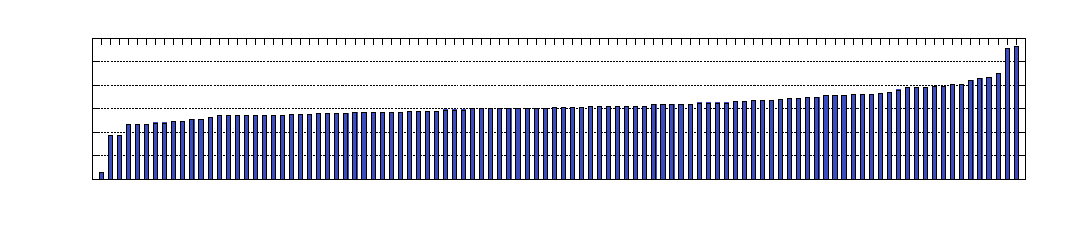
\includegraphics[width={504.00bp},height={100.80bp}]{images/hist_f42_with_Dx}}%
    \gplfronttext
  \end{picture}%
\endgroup
}
% 
%     \end{pspicture}
%     }
%     \caption{\textbf{Distribution discrepancy ratio:} Training–testing discrepancy differences across 102 UCR datasets, computed using metric equations introduced in Appendix~\ref{app:discrepancy:form}.}
%     \label{fig:datasets_variability}
% \end{figure*}
% 
% 
% 
% ========== Train/test discrepancy (ICML app:PerfMetrics:Discrepancy) ==========
\section{Discrepancy in distance between Training and Test sets}\label{app:discrepancy}\label{app:discrepancy:form}
To quantify the discrepancy between training and test distributions, we assess intra-class dispersion using Dynamic Time Warping (DTW) as the distance metric. For each class \( k \in \{1, \ldots, K\} \), let the set of time series in class \( k \) be denoted by \( \mathcal{X}_k = \{x_{k,1}, \ldots, x_{k,n_k}\} \), where \( n_k \) is the number of instances in class \( k \). Let \( \mu_k \) denote the DTW barycenter (i.e., the average sequence under DTW alignment) of \( \mathcal{X}_k \). The intra-class dispersion for class \( k \) is then defined as $d_k = \frac{1}{n_k} \sum_{i=1}^{n_k} \text{DTW}(x_{k,i}, \mu_k)$

The \textbf{Overall dataset dispersion} \( D \) is the mean intra-class dispersion across all \( K \) classes, defined by $D = \frac{1}{K} \sum_{k=1}^{K} d_k$, and \textbf{Discrepancy} is measured as the ratio of test to train set dispersions:$V = \frac{D_{\text{test}}}{D_{\text{train}}}$

The ratio \( V \) captures train-test diversity: \( V \approx 1 \) implies similar variability, \( V < 1 \) more dispersion in training, and \( V > 1 \) in testing. Datasets with \( V > 1 \) are more challenging for generative DA, highlighting the need for augmentation methods that extrapolate beyond the training distribution.


% \subsection{Experimental results}\label{app:discrepancy:results}
% The discrepancy ratios of the 102~UCR datasets have been plotted in ascending order in Figure~\ref{fig:datasets_variability}. Specifically, three datasets exemplify the extremes: \textbf{(i) Discrepancy towards test:} Dataset D8, \verb|Car| (ratio=1.53); \textbf{(ii) No discrepancy:} Dataset D20, \verb|ECGFiveDays| (1.00); \textbf{(iii) Discrepancy towards train:} Dataset D22, \verb|EOGVerticalSignal| (0.77). Detailed results of the discrepancies across the datasets are available in \tablename~\ref{Tab:app:Ablation_clustering_alpha}.








% \begin{table*}
% \centering
%  
% \label{tab:rounded_variability_metrics_part_3}
% \begin{tabular}{rlccc}
%                  \# &      $Dataset$ &  Ratio &    $Dispersion_{TEST}$ &   $Dispersion_{TRAIN}$ \\
% \toprule
% D101 & FacesUCR & 1.12 & $1.20\times10^{3}$ & $1.08\times10^{3}$ \\
% D102 & MiddlePhalanxOutlineAgeGroup & 1.12 & $2.70\times10^{1}$ & $2.24\times10^{1}$ \\
% D103 & Wafer & 1.12 & $2.24\times10^{2}$ & $2.30\times10^{2}$ \\
% D104 & ShapeletSim & 1.14 & $1.41\times10^{4}$ & $1.46\times10^{4}$ \\
% D105 & ArrowHead & 1.16 & $1.71\times10^{0}$ & $1.88\times10^{0}$ \\
% D106 & EOGHorizontalSignal & 1.18 & $3.01\times10^{1}$ & $2.65\times10^{1}$ \\
% D107 & ToeSegmentation1 & 1.18 & $2.19\times10^{2}$ & $2.16\times10^{2}$ \\
% D108 & SonyAIBORobotSurface2 & 1.18 & $2.80\times10^{1}$ & $2.36\times10^{1}$ \\
% D109 & MixedShapesSmallTrain & 1.19 & $1.59\times10^{2}$ & $1.55\times10^{2}$ \\
% D110 & ECG5000 & 1.19 & $4.17\times10^{1}$ & $4.77\times10^{1}$ \\
% D111 & ECG200 & 1.21 & $1.28\times10^{2}$ & $1.25\times10^{2}$ \\
% D112 & DistalPhalanxOutlineAgeGroup & 1.21 & $6.78\times10^{1}$ & $6.71\times10^{1}$ \\
% D113 & CinCECGTorso & 1.24 & $1.41\times10^{1}$ & $1.40\times10^{1}$ \\
% D114 & PickupGestureWiimoteZ & 1.25 & $5.23\times10^{0}$ & $5.98\times10^{0}$ \\
% D115 & InsectEPGRegularTrain & 1.26 & $1.88\times10^{1}$ & $1.94\times10^{1}$ \\
% D116 & Rock & 1.27 & $1.16\times10^{2}$ & $1.11\times10^{2}$ \\
% D117 & BirdChicken & 1.30 & $5.28\times10^{1}$ & $5.47\times10^{1}$ \\
% D118 & PigArtPressure & 1.38 & $1.03\times10^{2}$ & $9.85\times10^{1}$ \\
% D119 & Phoneme & 1.50 & $5.18\times10^{1}$ & $4.70\times10^{1}$ \\
% D120 & Car & 1.51 & $3.94\times10^{2}$ & $3.95\times10^{2}$ \\
% D121 & PigCVP & 1.52 & $6.68\times10^{1}$ & $6.54\times10^{1}$ \\
% D122 & Symbols & 1.53 & $1.23\times10^{1}$ & $3.72\times10^{0}$ \\
% D123 & PigAirwayPressure & 2.07 & $7.11\times10^{2}$ & $5.72\times10^{2}$ \\
% D124 & DiatomSizeReduction & 3.30 & $1.52\times10^{3}$ & $1.00\times10^{3}$ \\
% \bottomrule
% \end{tabular}
% \end{table*}



% % Dataset Diversity
% \begin{figure*}[t]
%     \centering 
%     \includegraphics[width=\linewidth,clip=true,trim=0cm 0cm 0cm 0cm]{images/datasets_variability.pdf}
%     %\input{images/cumulative_sum_discrepency}
%     \caption{\textbf{Distribution discrepancy ratio:} Overview of the difference in discrepancy between training and testing sets of the $102$ UCR datasets; discrepancy ratio computed using \eqref{eq:variability_ratio}}.
%     \label{fig:datasets_variability}
% \end{figure*}


% % Time-series features
% \input{sections/appendix/time_series_features}
% \newpage
% Latent Space Evolution
% \input{sections/appendix/latent_space_evolution}


% ========== Latent space evolution (ICML app:Exp:LatentS_Evolution) ==========
\iffalse  % --- Appendix L (Latent space evolution) commented out ---
\section{Evolution of latent space through learning phase} \label{app:latent_evolution}
Latent space visualizations via PCA projection in \tablename~\ref{Fig:LatentS} highlight how augmentation affects distribution modeling: initial clusters are well-separated, but iterative steps increase density and exploration. Later, inter-class distances shrink, making further exploration harder. These insights are limited by the 3D projection of the original 50-dimensional space.


%A progressive visualization of the latent space offers valuable insights into the evolving distribution modeling and exploration process. Initially, the latent space representations exhibit fine clustering, but as we iterate in the augmentation loop, the latent space distributions become denser, enhancing the exploration part of these distributions. However, in the later stages of augmentation, the exploration process becomes increasingly challenging as the inter-class distances appear to shrink due to prior augmentation steps. It is important to note that these visualizations provide only a limited view of the actual distributions, as they are restricted to three dimensions (from an original 50-dimensional space).

% Synthetic data diversity by method

\begin{table*}[t]
\centering
\caption{Latent Space Evolution: Visualization of the first 3 dimensions of the PCA over 50-D latent space.}\label{Fig:LatentS}
\begin{tabular}{ccccc}

\toprule
\bf Step & \bf ACSF1 & \bf BeetleFly & \bf Car & \bf ECG200 \\ 
\midrule
Original & 
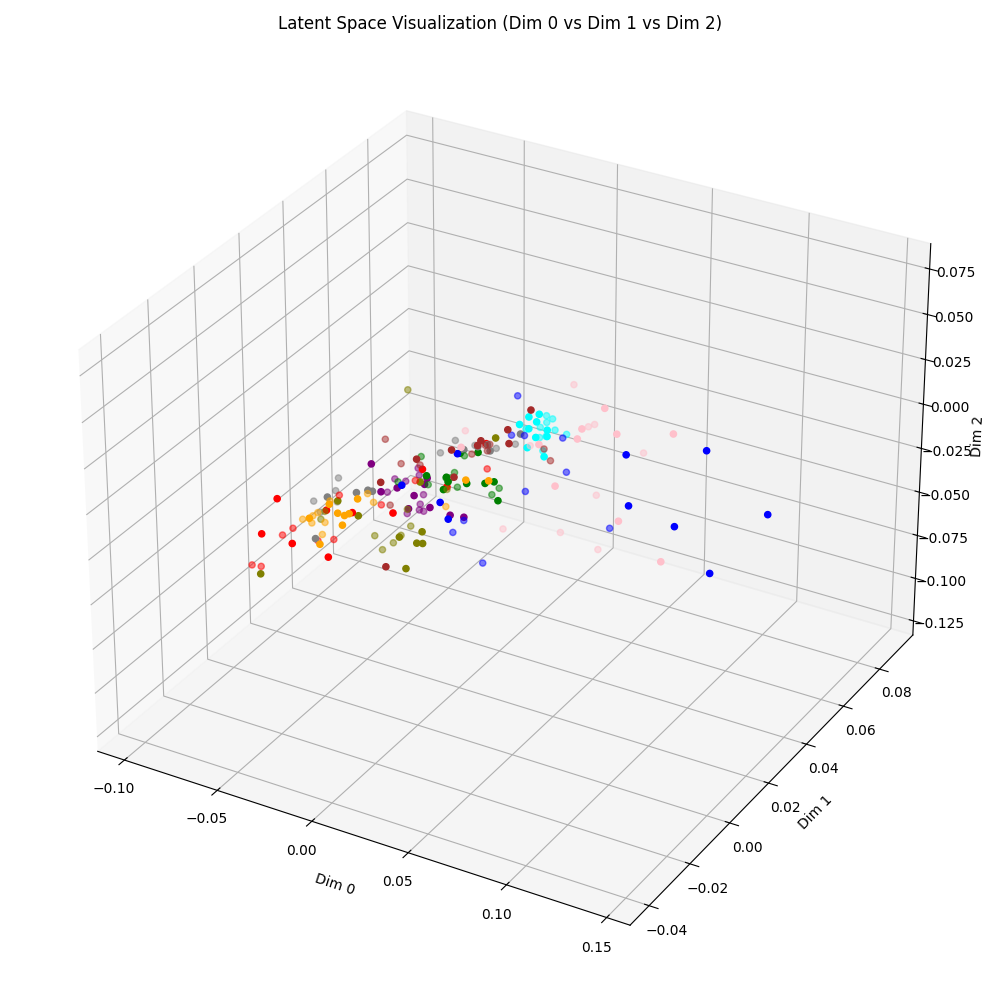
\includegraphics[width=\imgsize]{images/latent_space_viz_dataset_ACSF1.png} & 
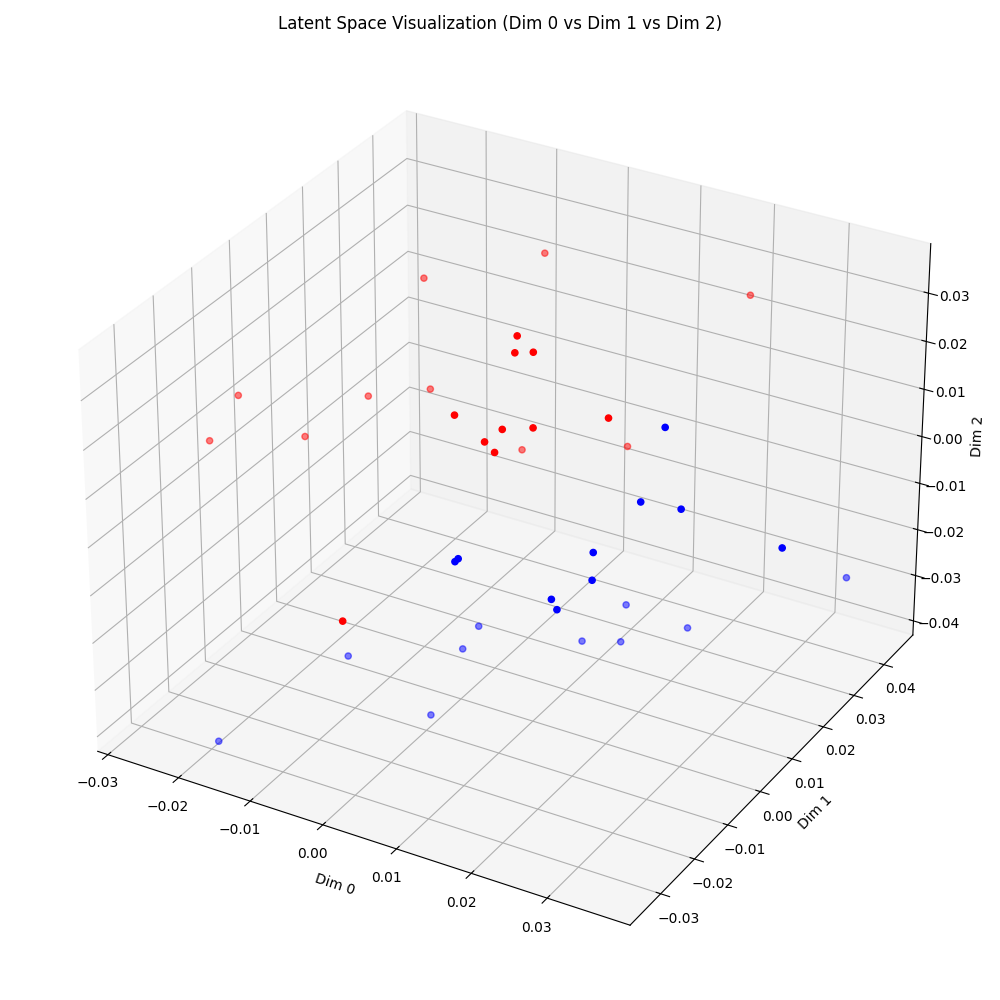
\includegraphics[width=\imgsize]{images/latent_space_viz_dataset_BeetleFly.png} & 
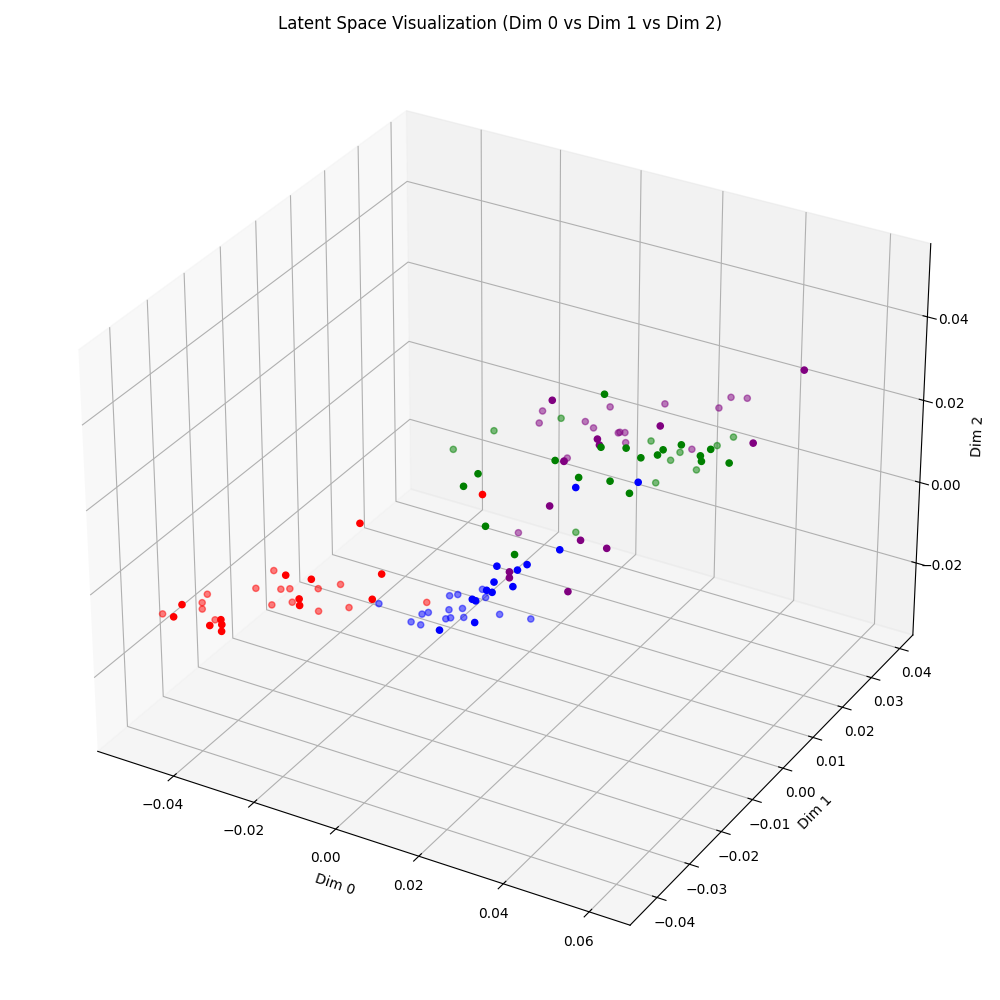
\includegraphics[width=\imgsize]{images/latent_space_viz_dataset_Car.png} & 
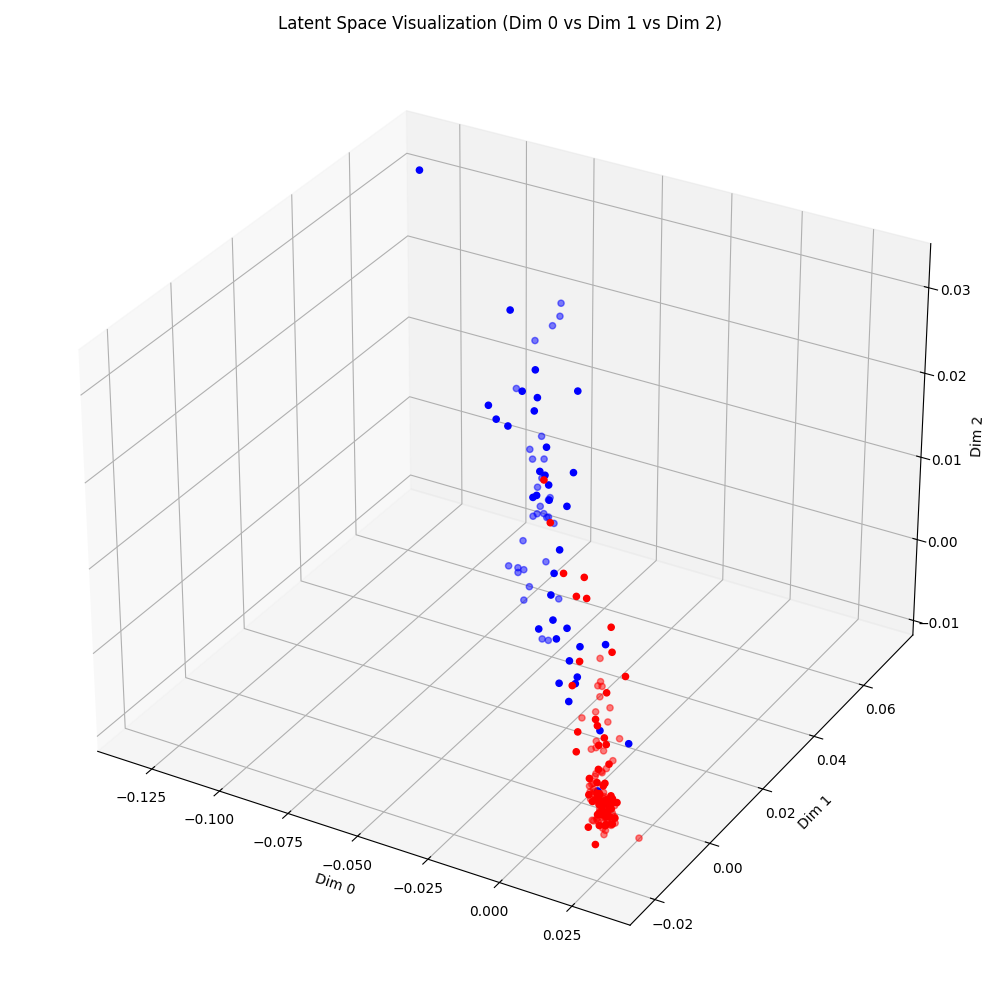
\includegraphics[width=\imgsize]{images/latent_space_viz_dataset_ECG200.png} \\ 

Step 0 & 
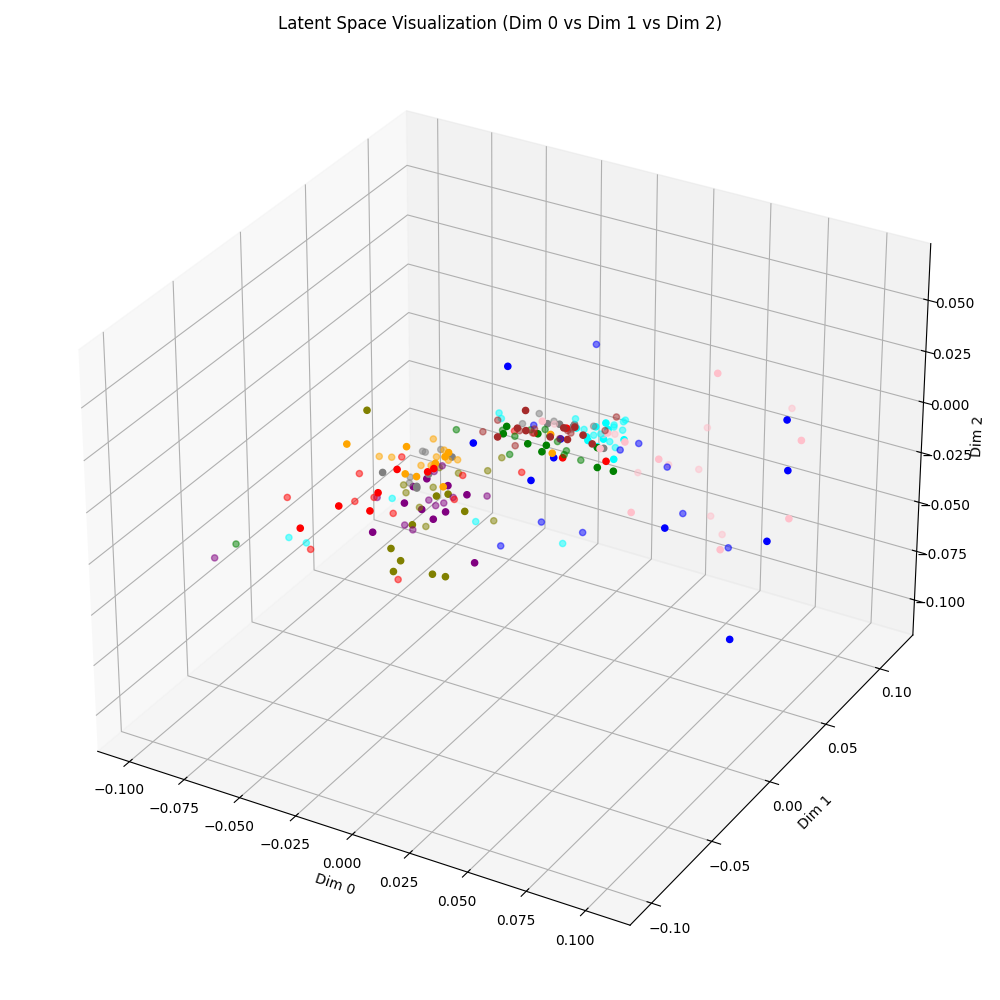
\includegraphics[width=\imgsize]{images/latent_space_viz_dataset_ACSF1_augmented_step_0.png} & 
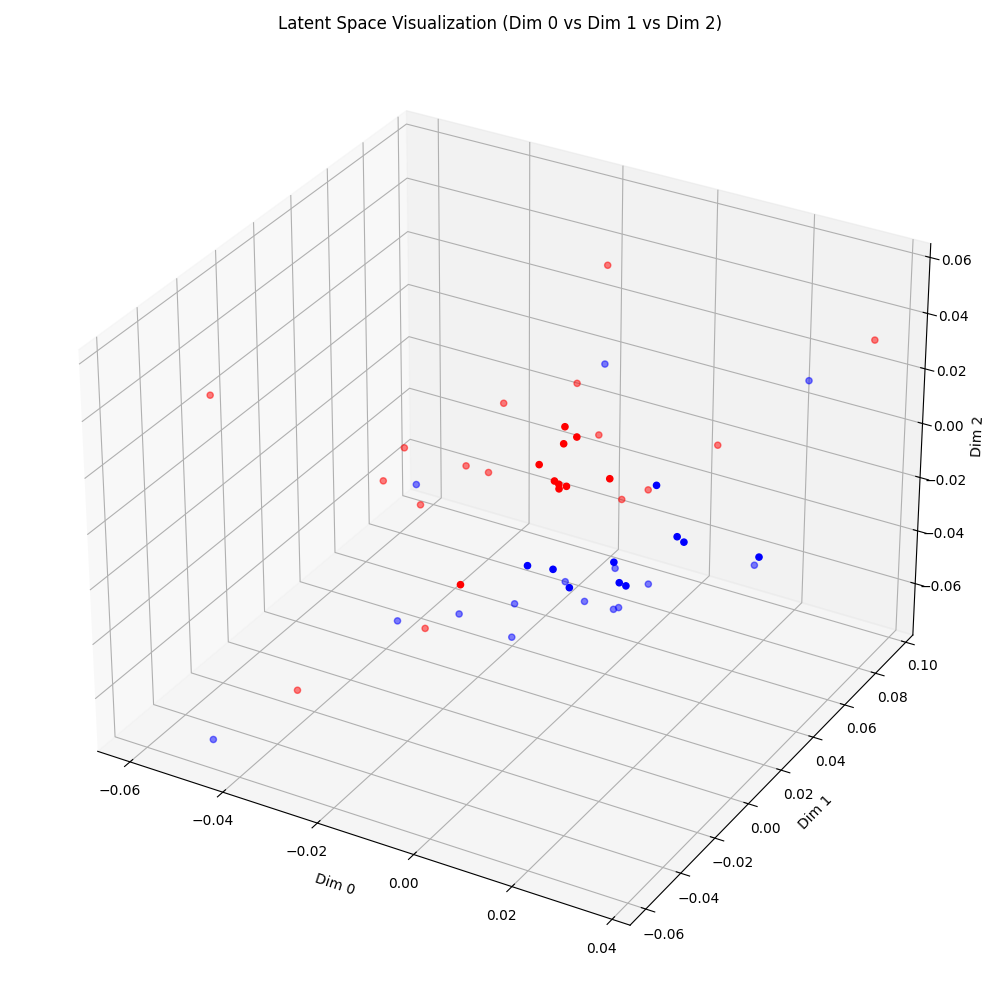
\includegraphics[width=\imgsize]{images/latent_space_viz_dataset_BeetleFly_augmented_step_0.png} & 
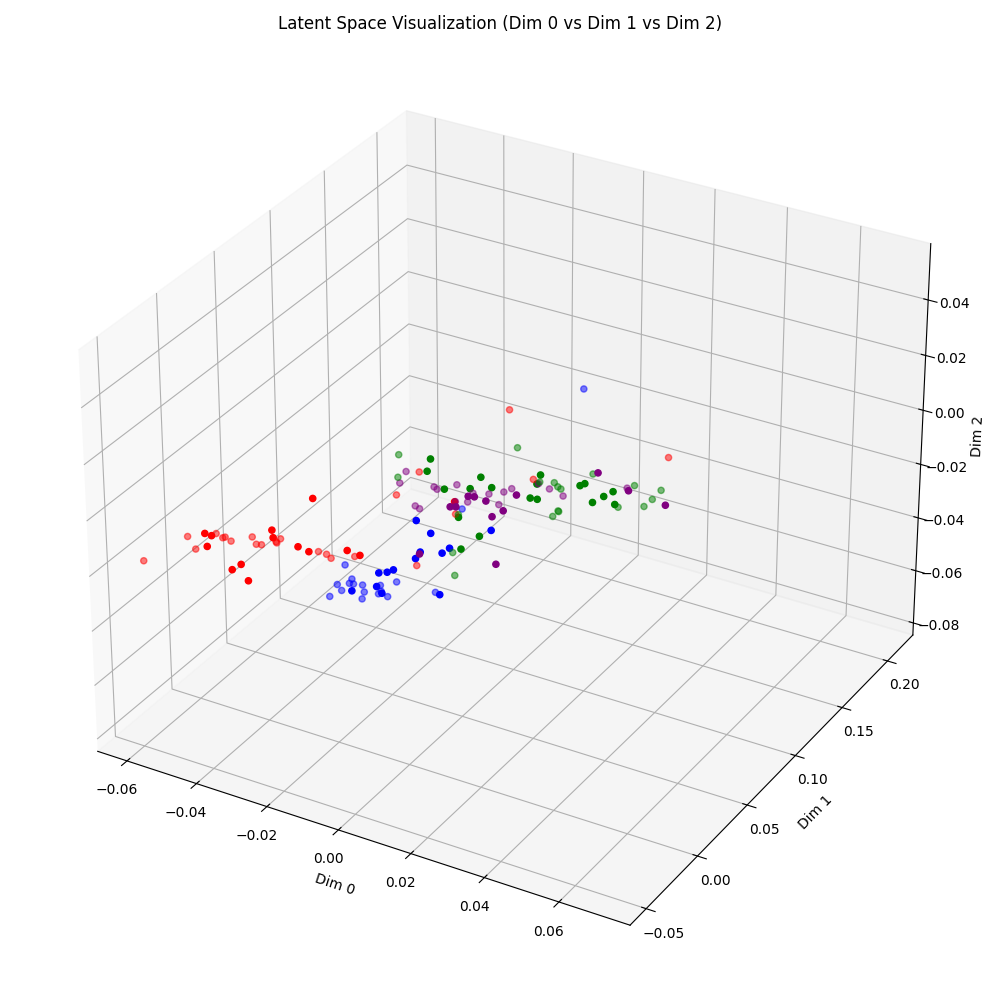
\includegraphics[width=\imgsize]{images/latent_space_viz_dataset_Car_augmented_step_0.png} & 
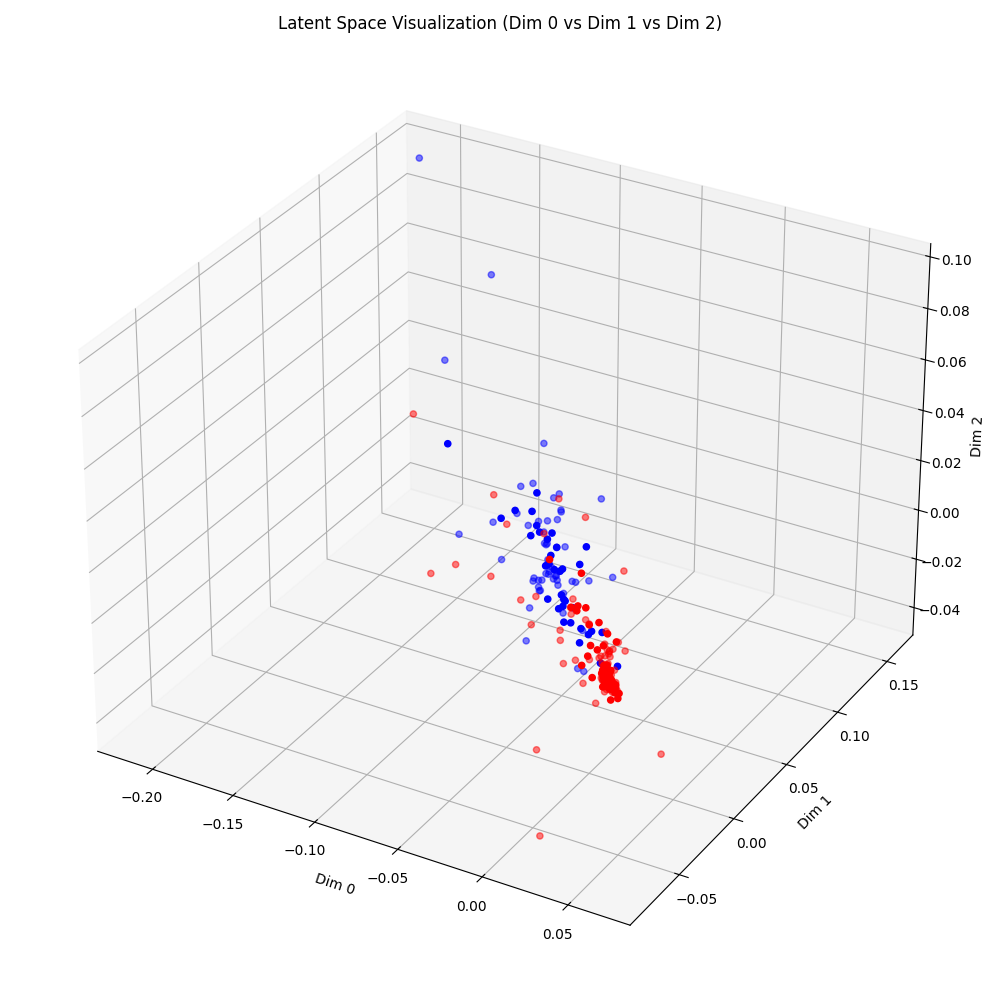
\includegraphics[width=\imgsize]{images/latent_space_viz_dataset_ECG200_augmented_step_0.png} \\ 

Step 1 & 
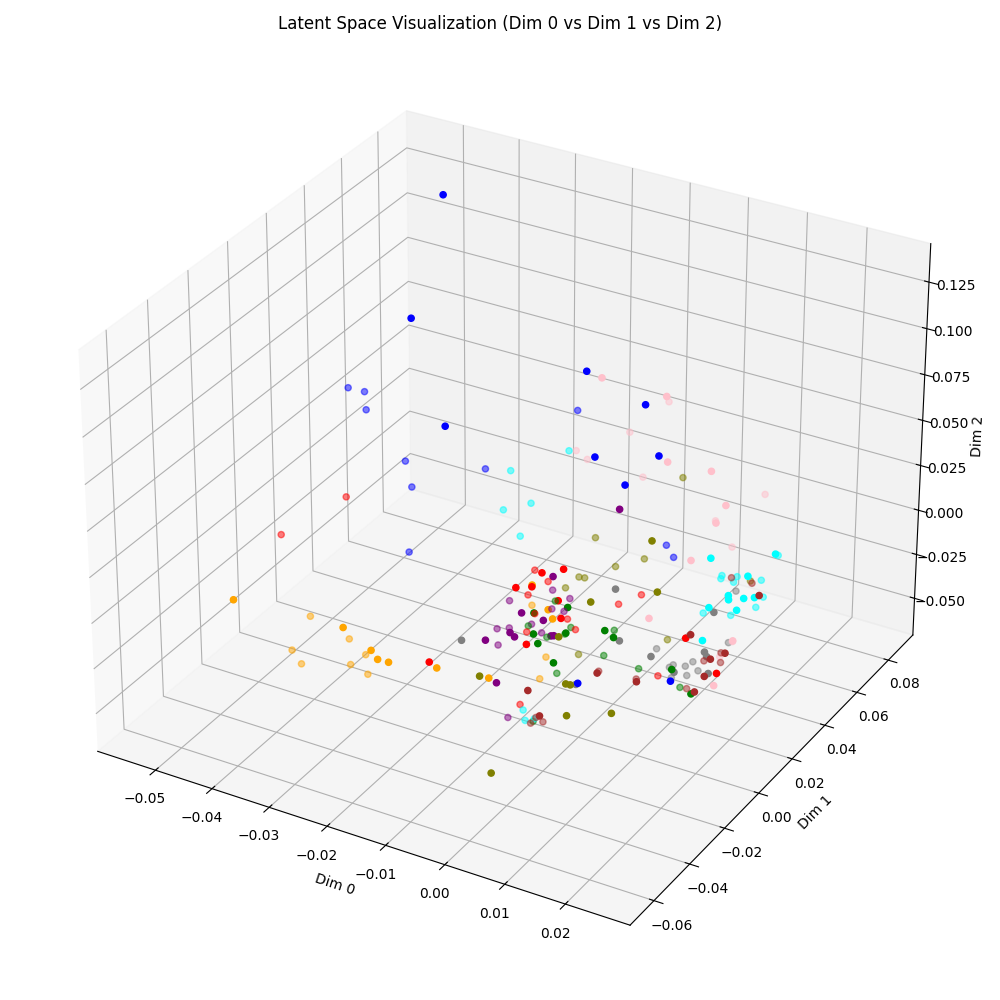
\includegraphics[width=\imgsize]{images/latent_space_viz_dataset_ACSF1_augmented_step_1.png} & 
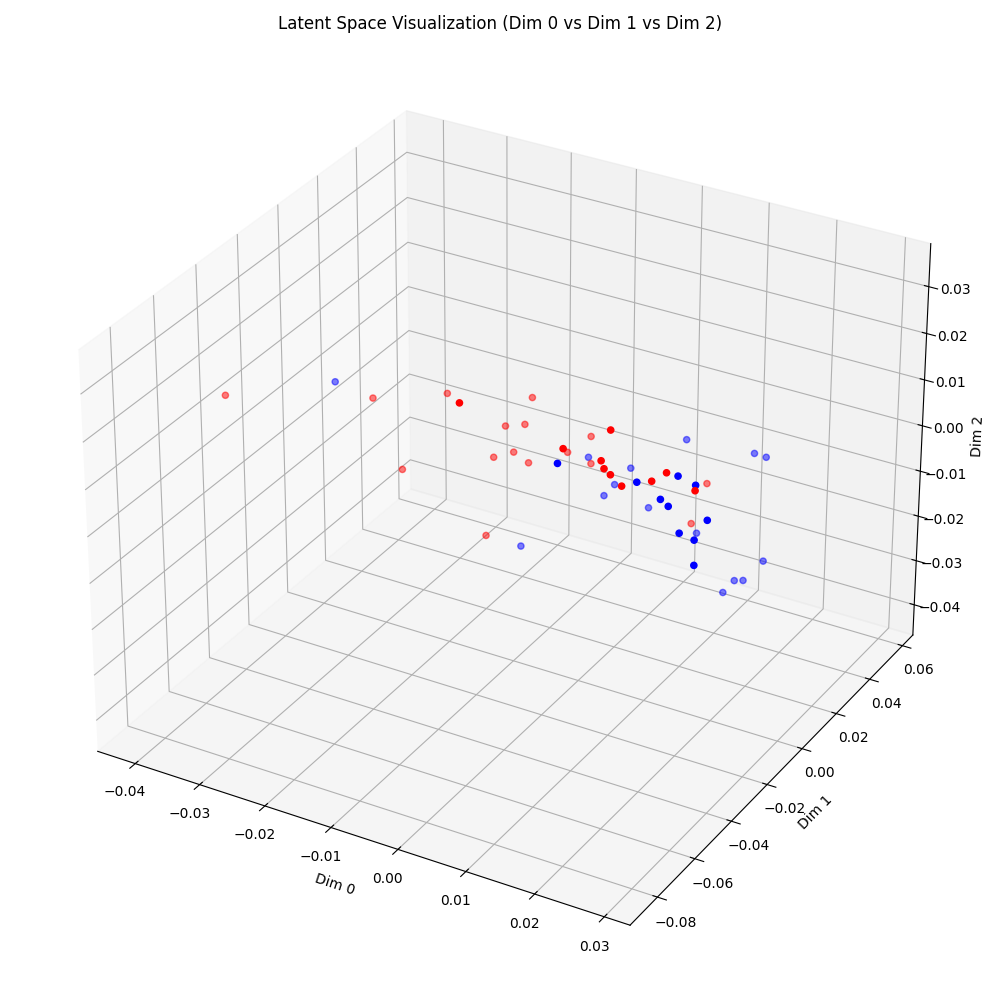
\includegraphics[width=\imgsize]{images/latent_space_viz_dataset_BeetleFly_augmented_step_1.png} & 
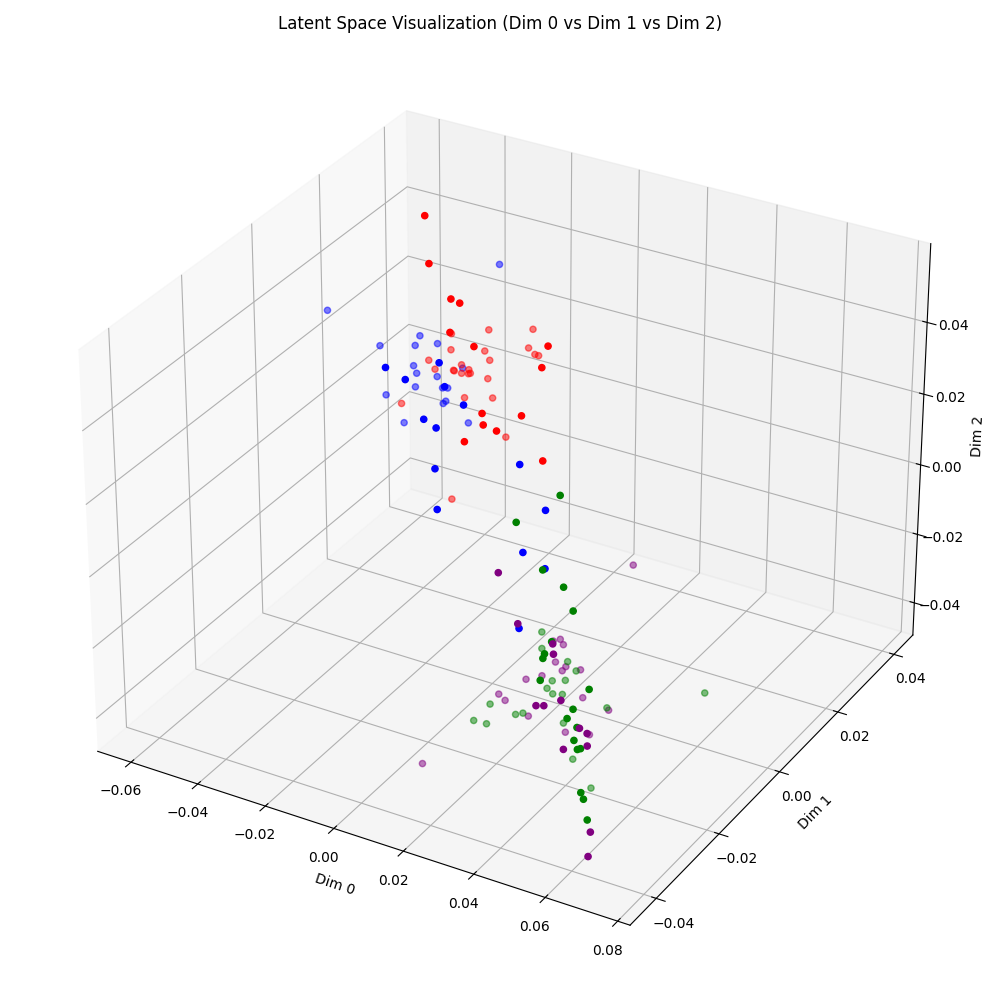
\includegraphics[width=\imgsize]{images/latent_space_viz_dataset_Car_augmented_step_1.png} & 
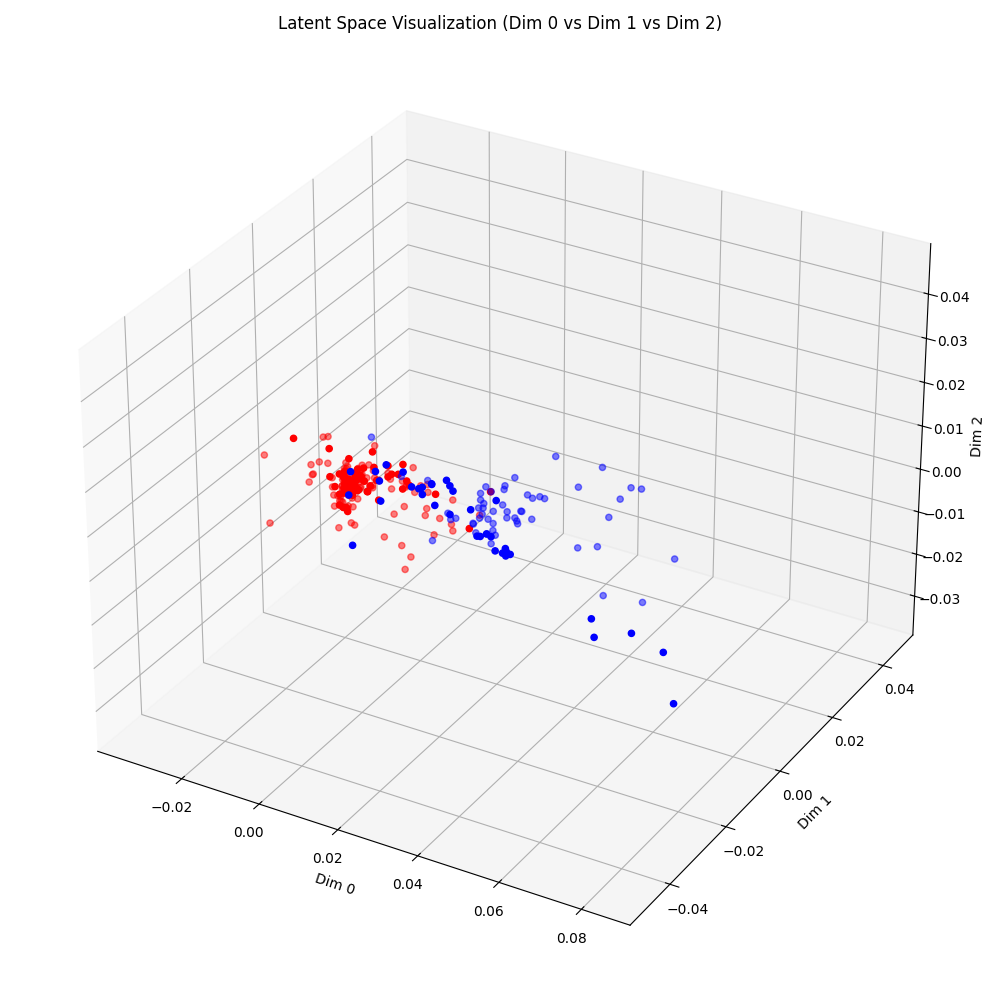
\includegraphics[width=\imgsize]{images/latent_space_viz_dataset_ECG200_augmented_step_1.png} \\ 

Step 2 & 
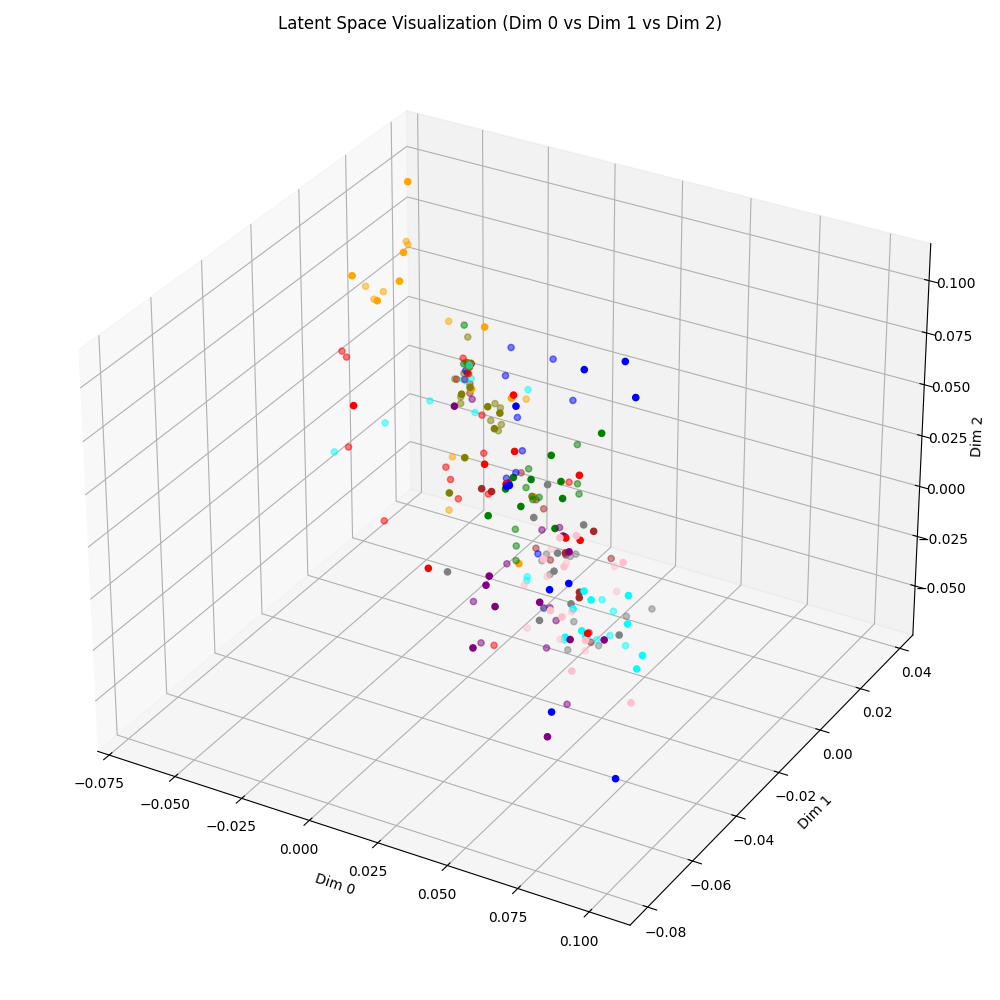
\includegraphics[width=\imgsize]{images/latent_space_viz_dataset_ACSF1_augmented_step_2.png} & 
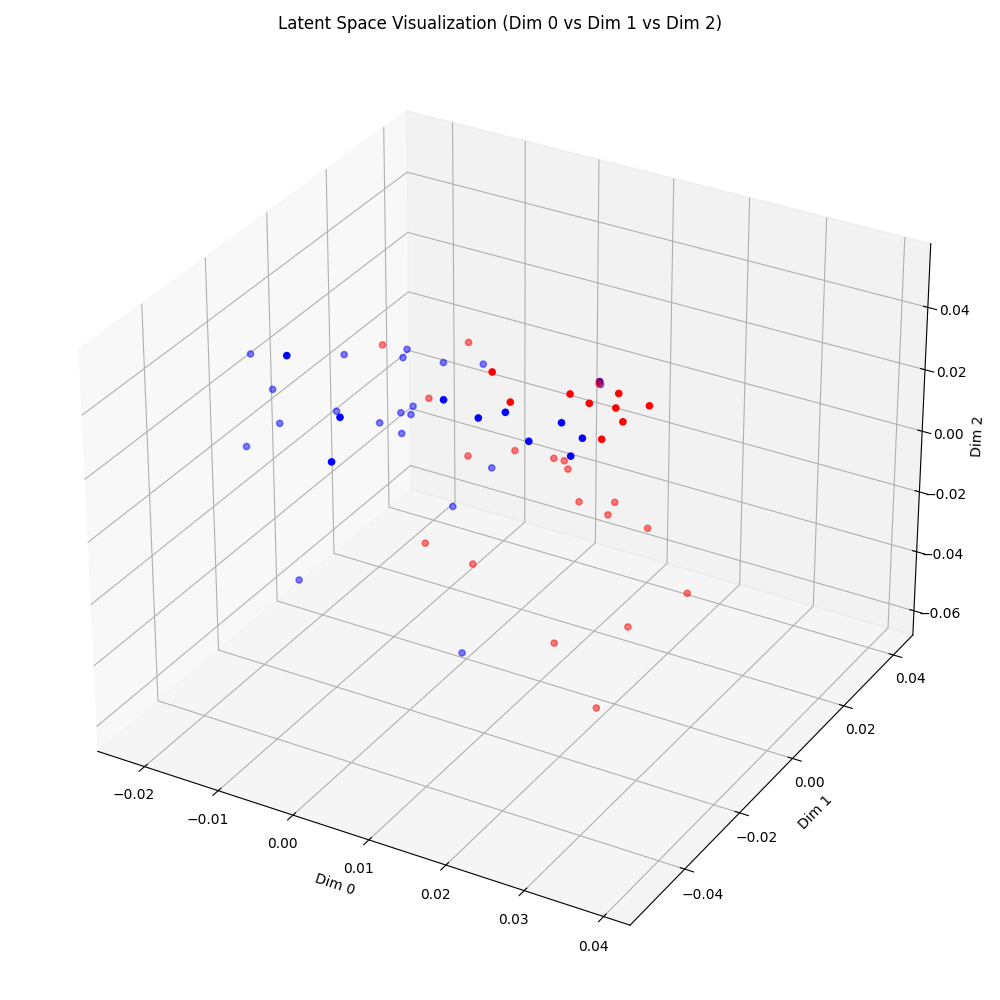
\includegraphics[width=\imgsize]{images/latent_space_viz_dataset_BeetleFly_augmented_step_2.png} & 
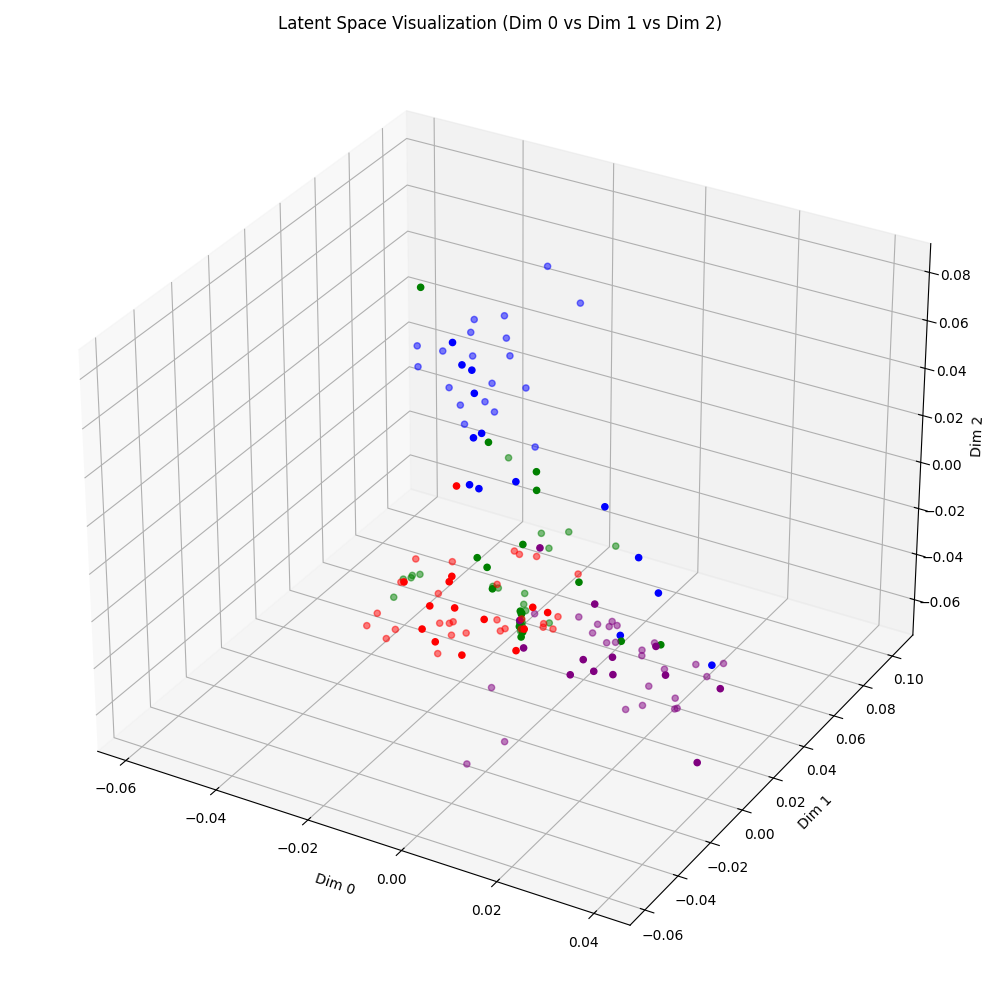
\includegraphics[width=\imgsize]{images/latent_space_viz_dataset_Car_augmented_step_2.png} & 
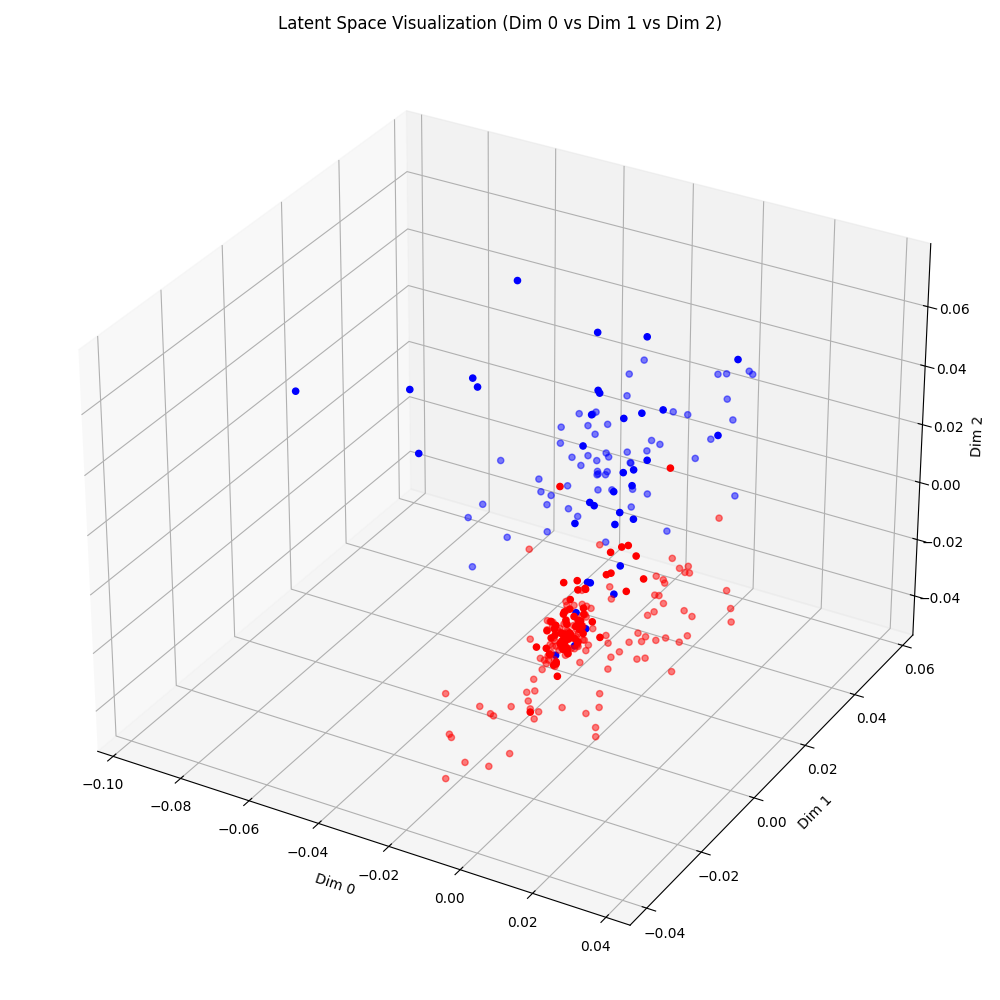
\includegraphics[width=\imgsize]{images/latent_space_viz_dataset_ECG200_augmented_step_2.png} \\ 

Step 3 & 
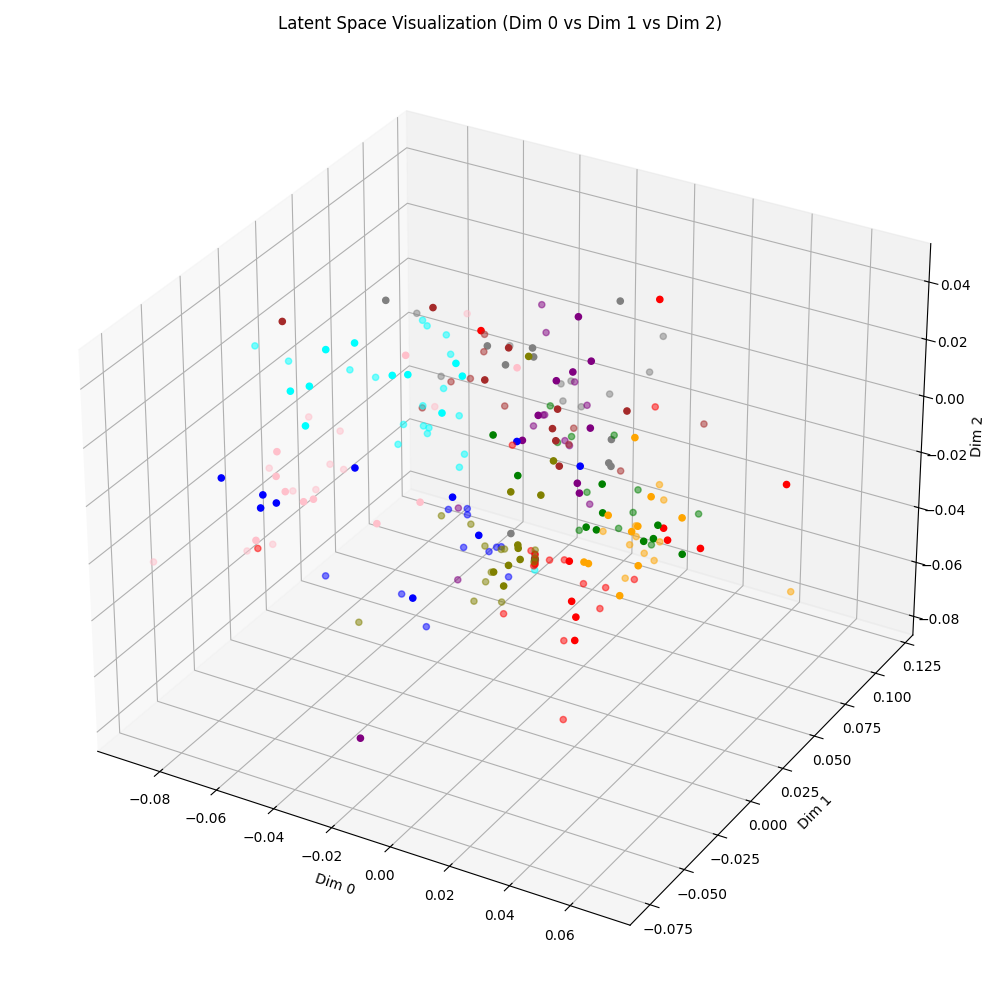
\includegraphics[width=\imgsize]{images/latent_space_viz_dataset_ACSF1_augmented_step_3.png} & 
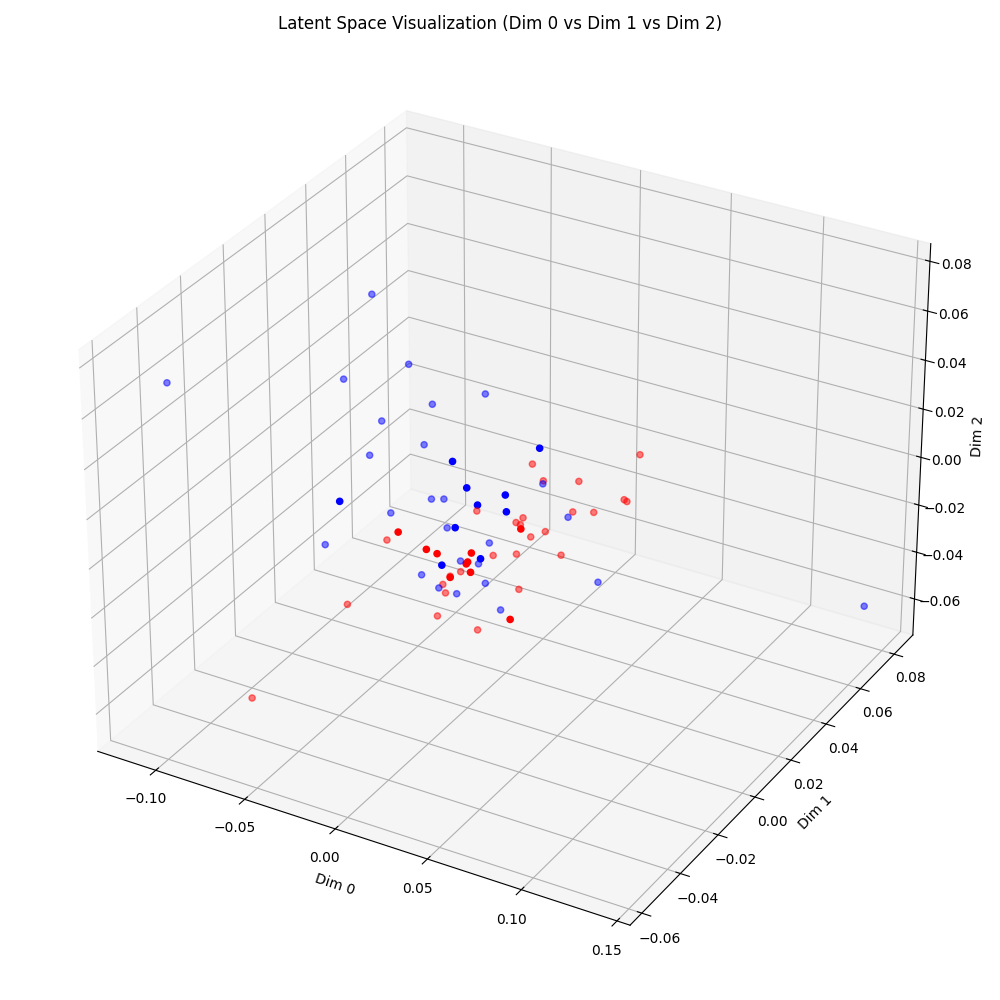
\includegraphics[width=\imgsize]{images/latent_space_viz_dataset_BeetleFly_augmented_step_3.png} & 
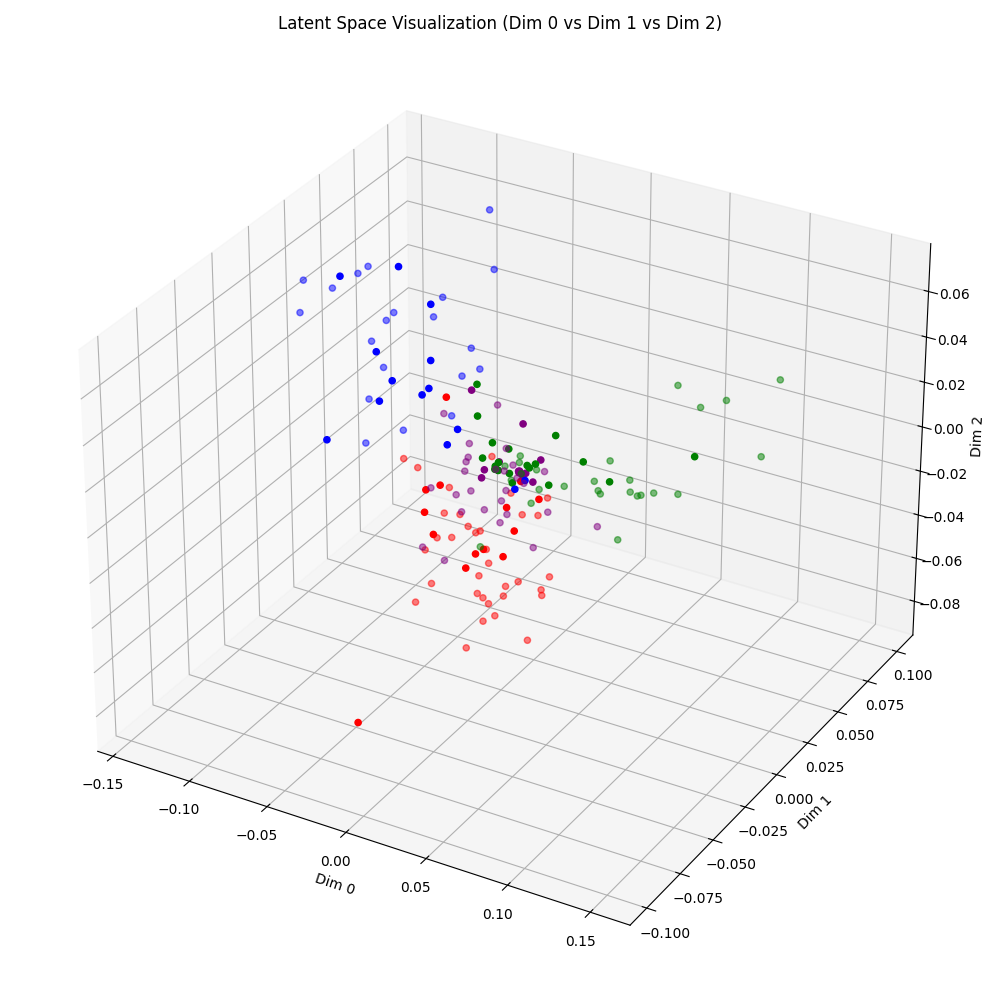
\includegraphics[width=\imgsize]{images/latent_space_viz_dataset_Car_augmented_step_3.png} & 
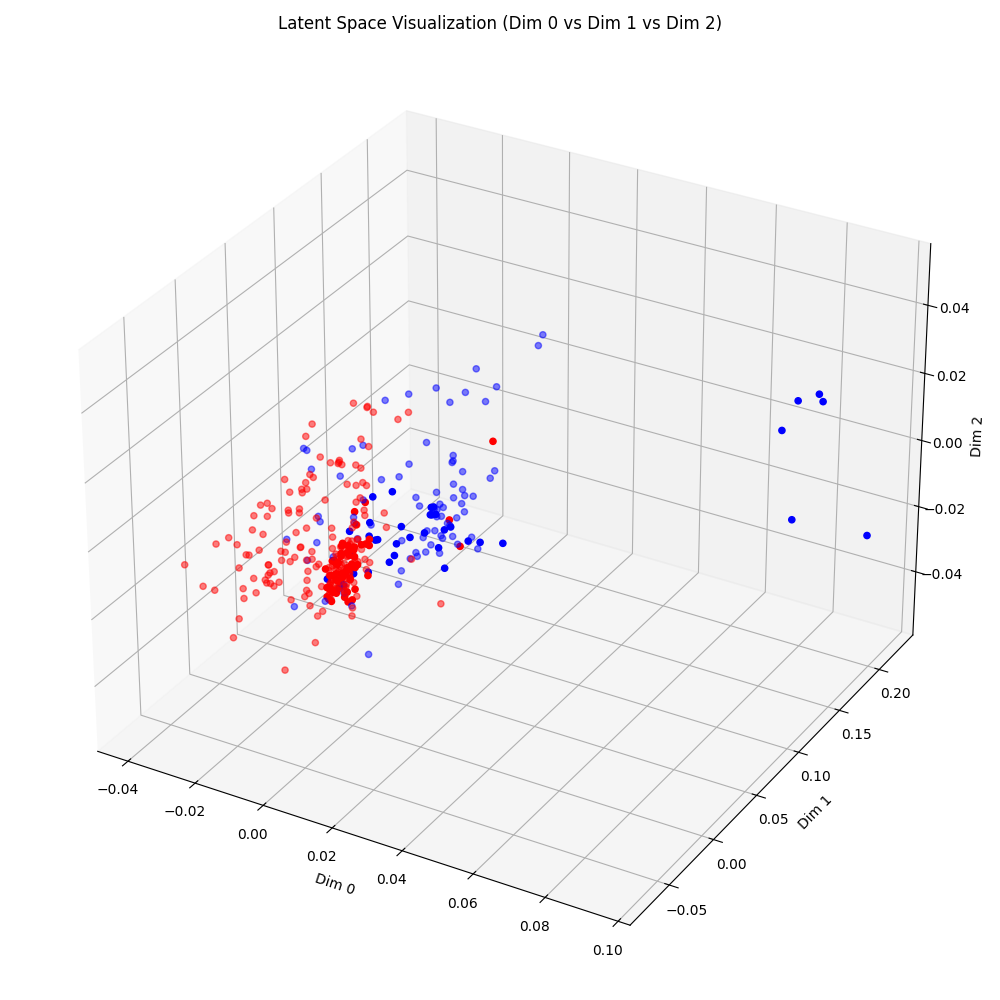
\includegraphics[width=\imgsize]{images/latent_space_viz_dataset_ECG200_augmented_step_3.png} \\ 

Step 4 & 
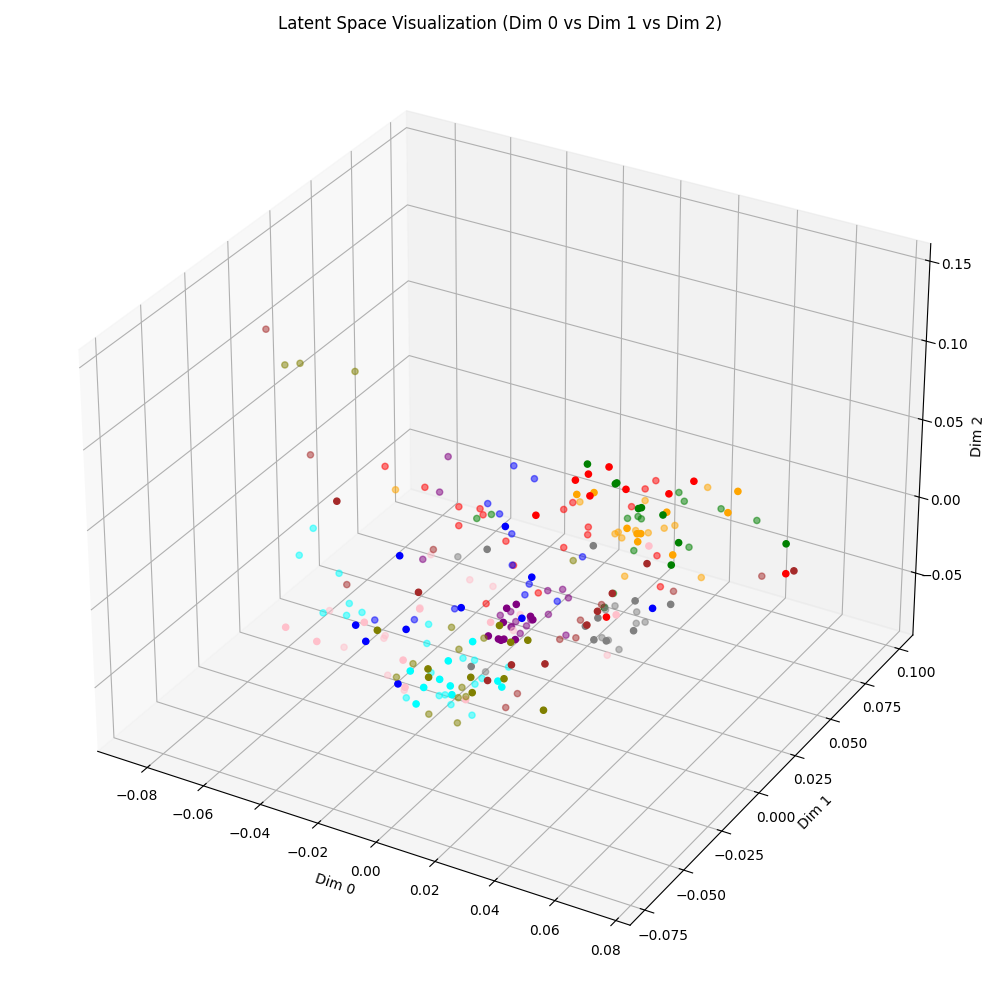
\includegraphics[width=\imgsize]{images/latent_space_viz_dataset_ACSF1_augmented_step_4.png} & 
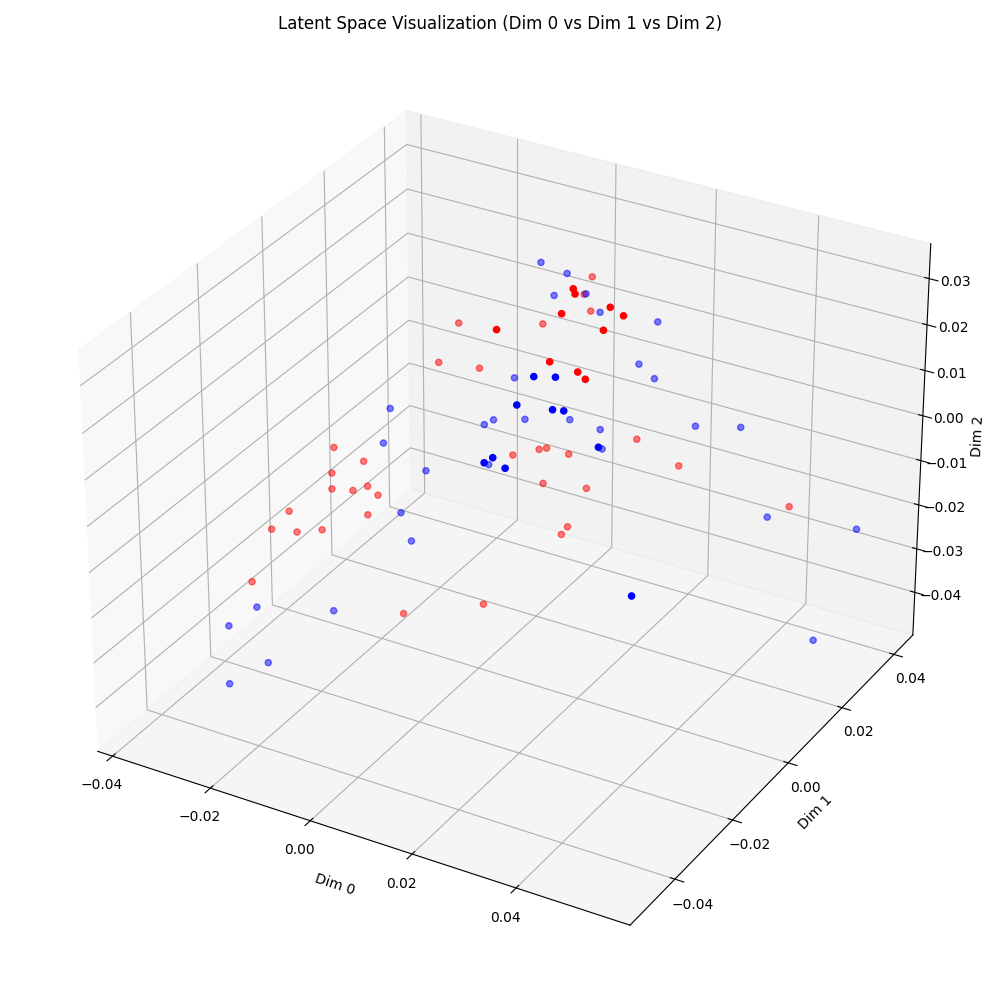
\includegraphics[width=\imgsize]{images/latent_space_viz_dataset_BeetleFly_augmented_step_4.png} & 
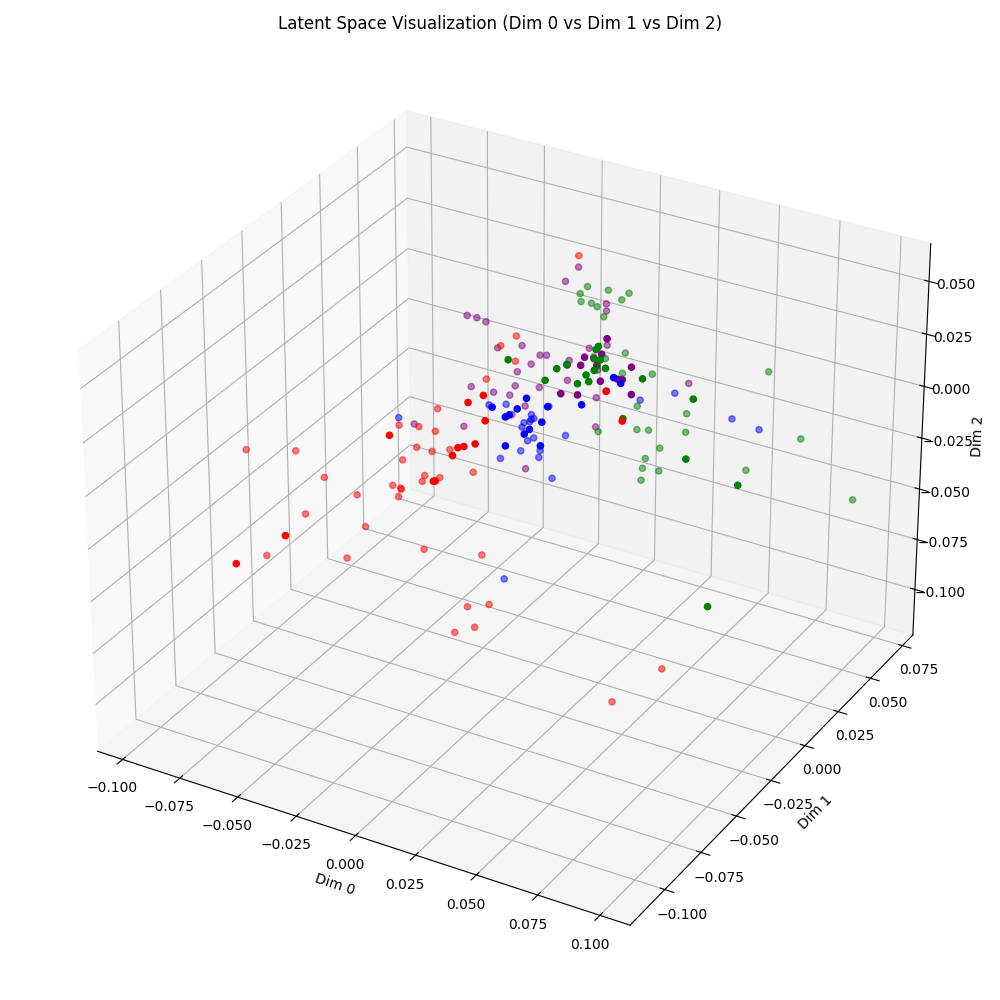
\includegraphics[width=\imgsize]{images/latent_space_viz_dataset_Car_augmented_step_4.png} & 
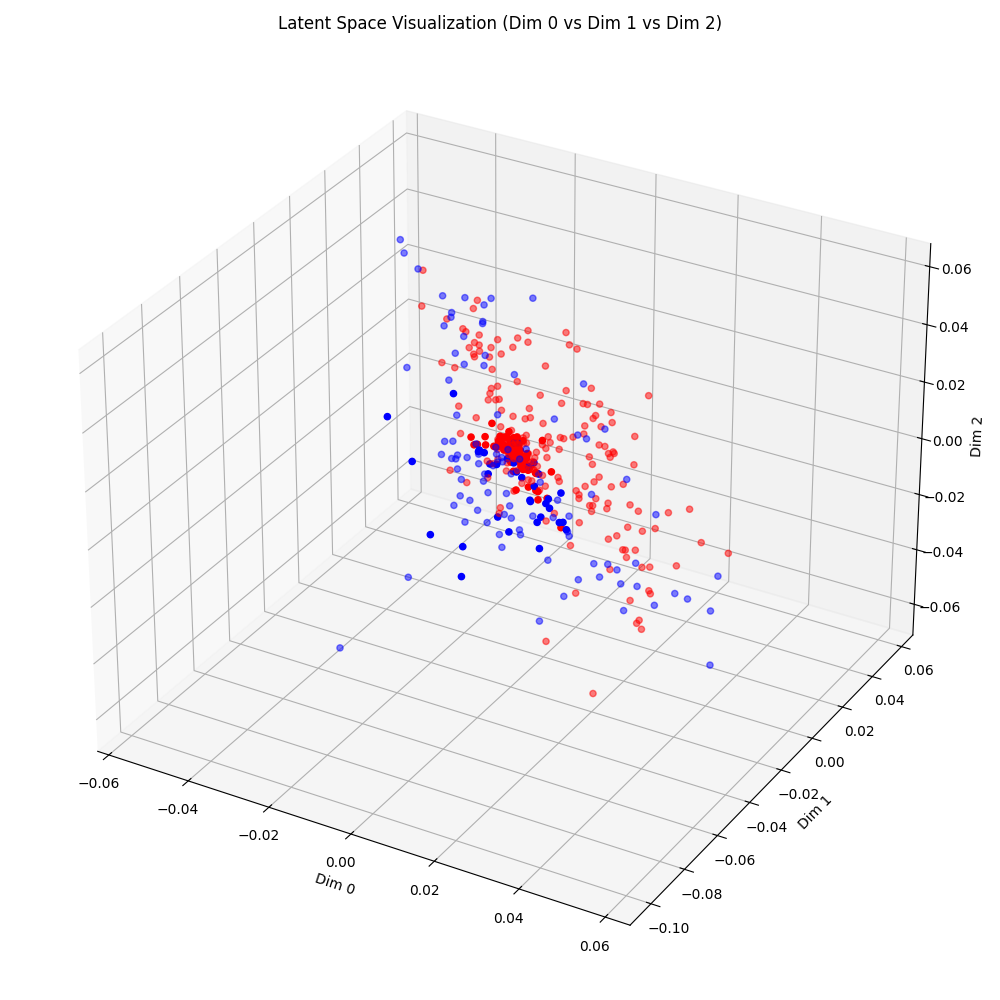
\includegraphics[width=\imgsize]{images/latent_space_viz_dataset_ECG200_augmented_step_4.png} \\ 

Step 5 & 
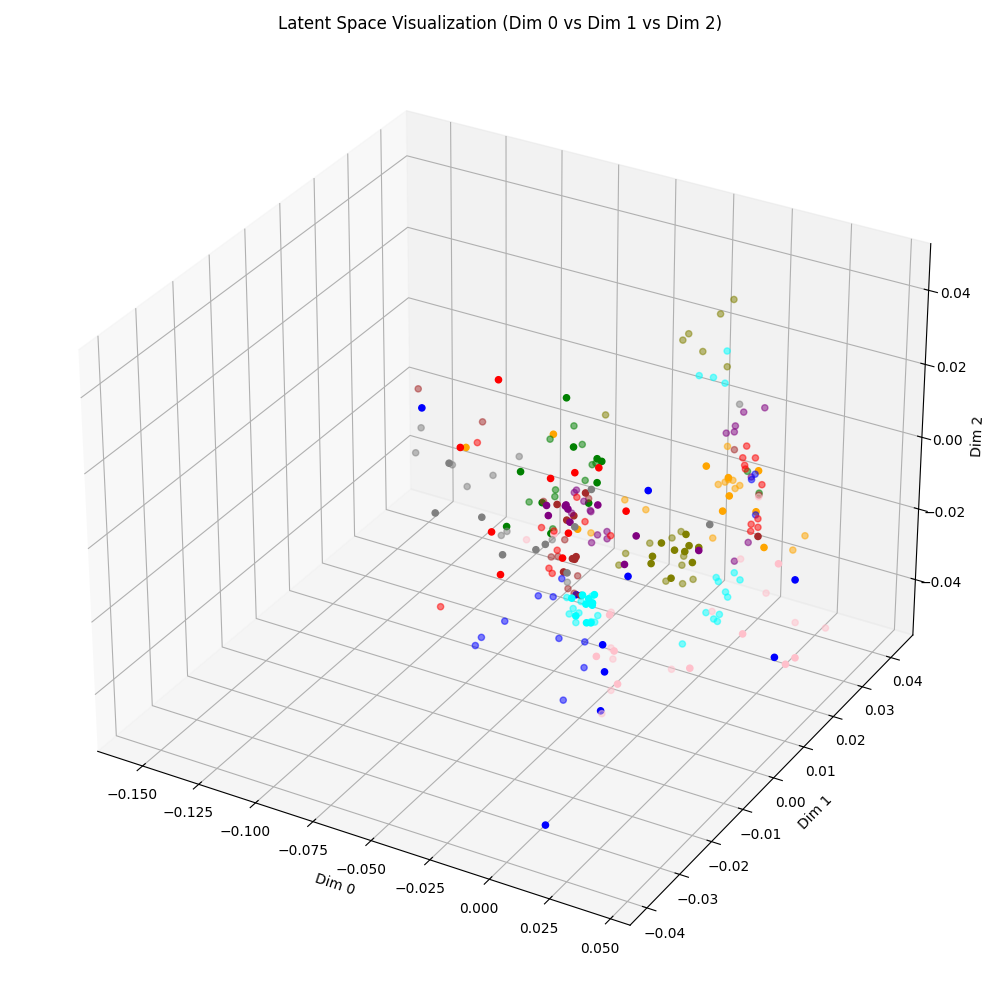
\includegraphics[width=\imgsize]{images/latent_space_viz_dataset_ACSF1_augmented_step_5.png} & 
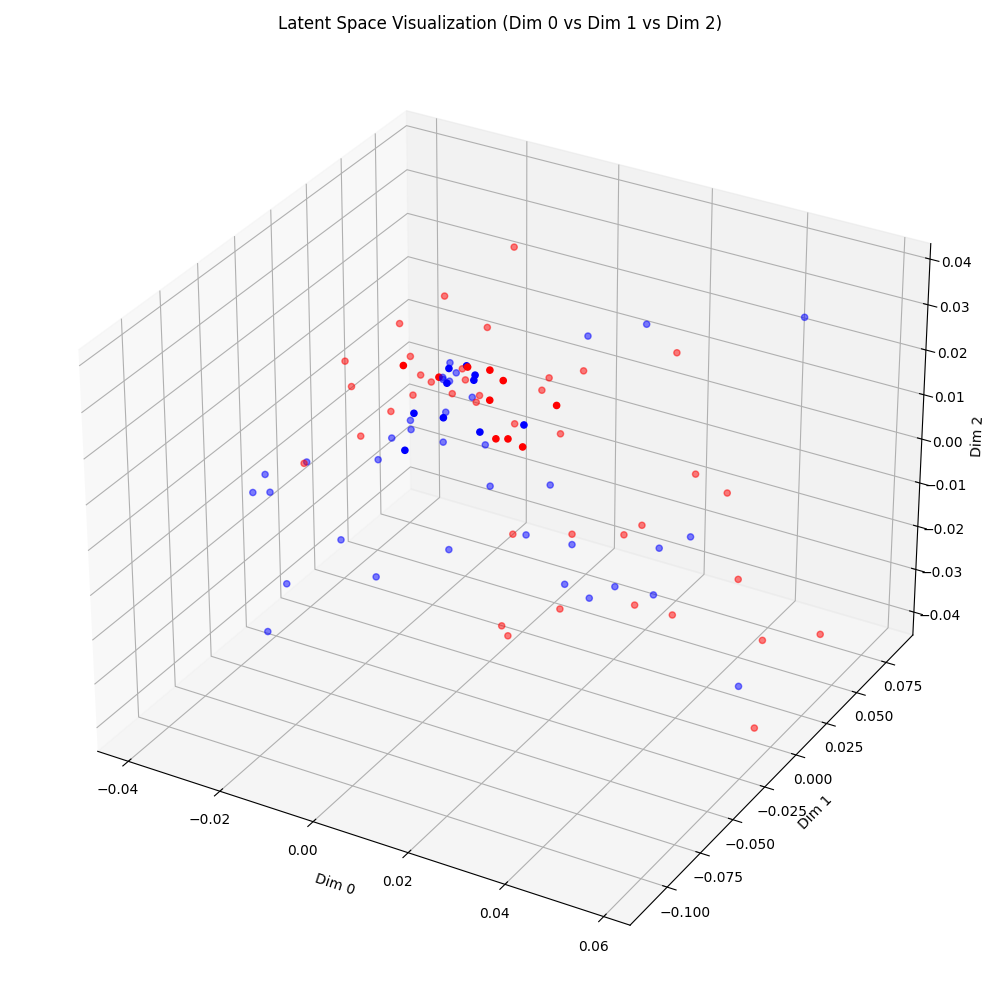
\includegraphics[width=\imgsize]{images/latent_space_viz_dataset_BeetleFly_augmented_step_5.png} & 
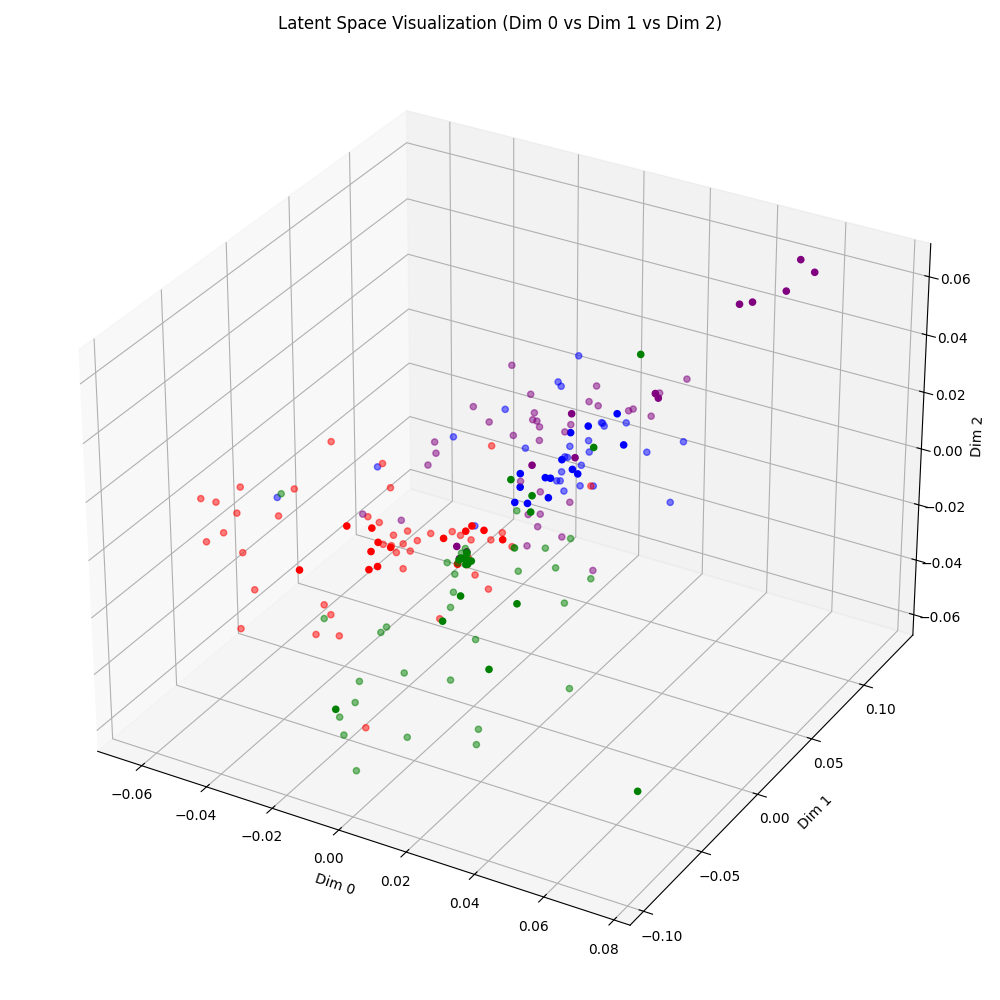
\includegraphics[width=\imgsize]{images/latent_space_viz_dataset_Car_augmented_step_5.png} & 
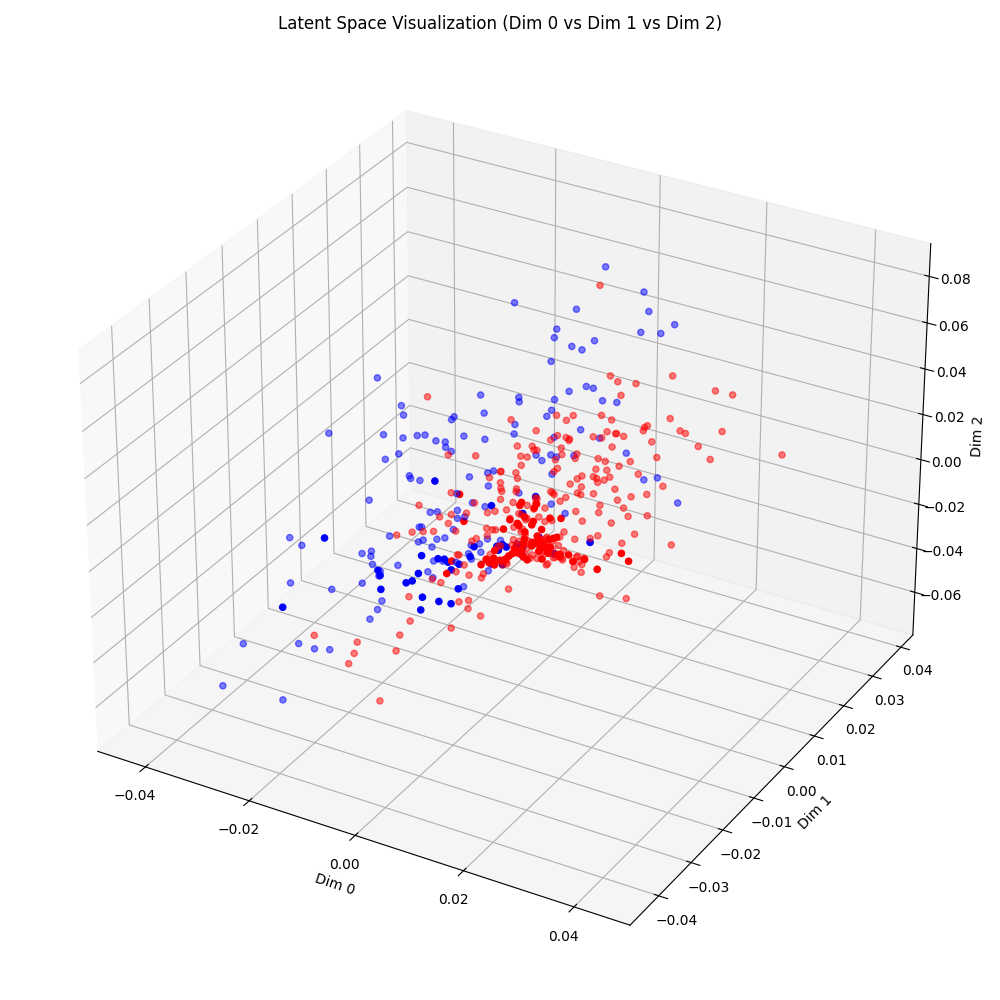
\includegraphics[width=\imgsize]{images/latent_space_viz_dataset_ECG200_augmented_step_5.png} \\ 
\bottomrule
\end{tabular}

\end{table*}

\newpage


\begin{table*}[t]
\centering
\begin{tabular}{ccccc}
\toprule
\bf Step & \bf EOGVerticalSignal & \bf Ham & \bf PigArtPressure & \bf SemgHandMov.Ch2 \\ 
\midrule
Original & 
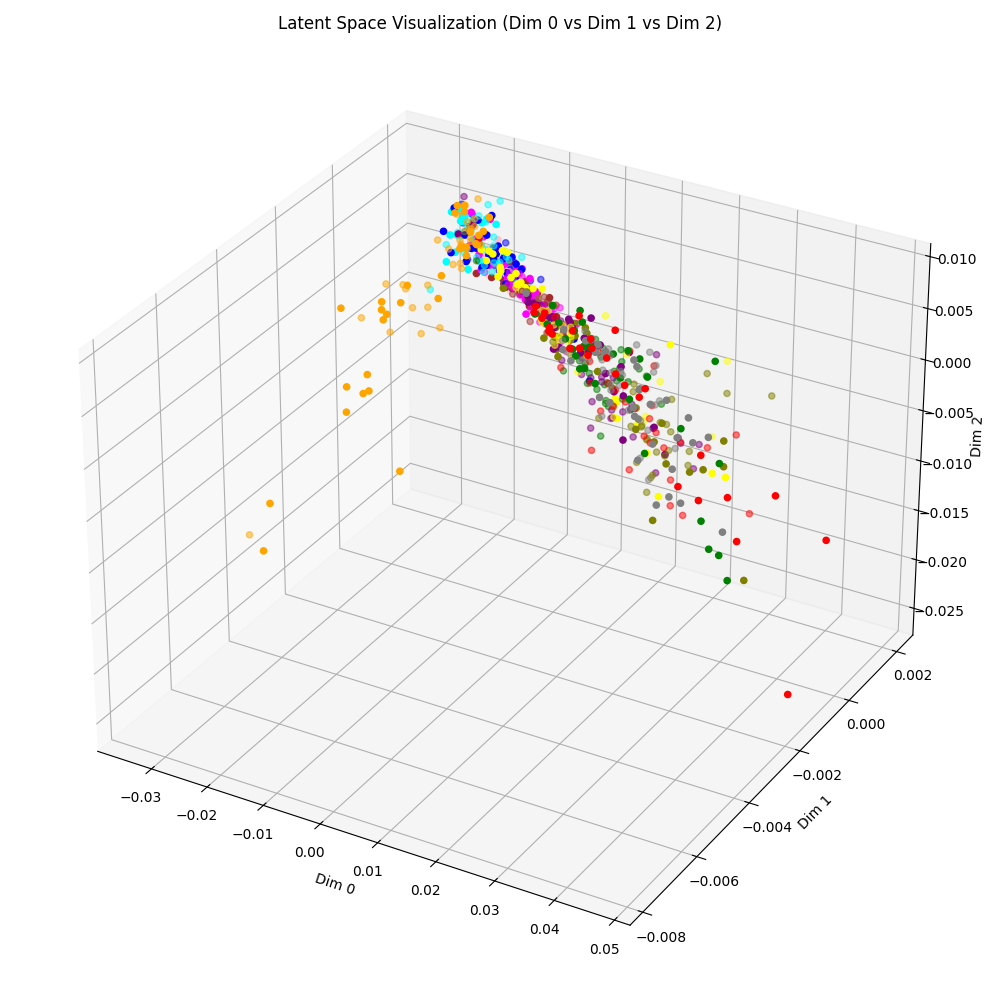
\includegraphics[width=\imgsize]{images/latent_space_viz_dataset_EOGVerticalSignal_original.png} & 
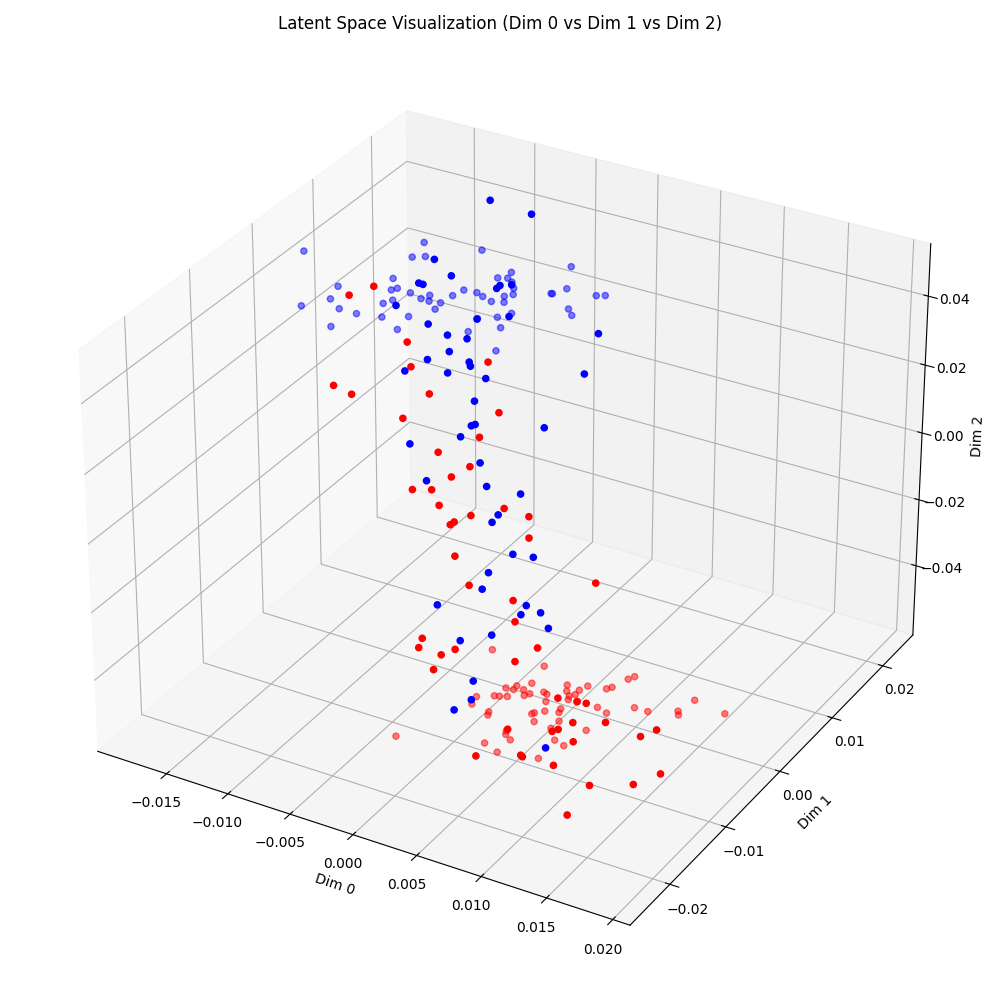
\includegraphics[width=\imgsize]{images/latent_space_viz_dataset_Ham.png} & 
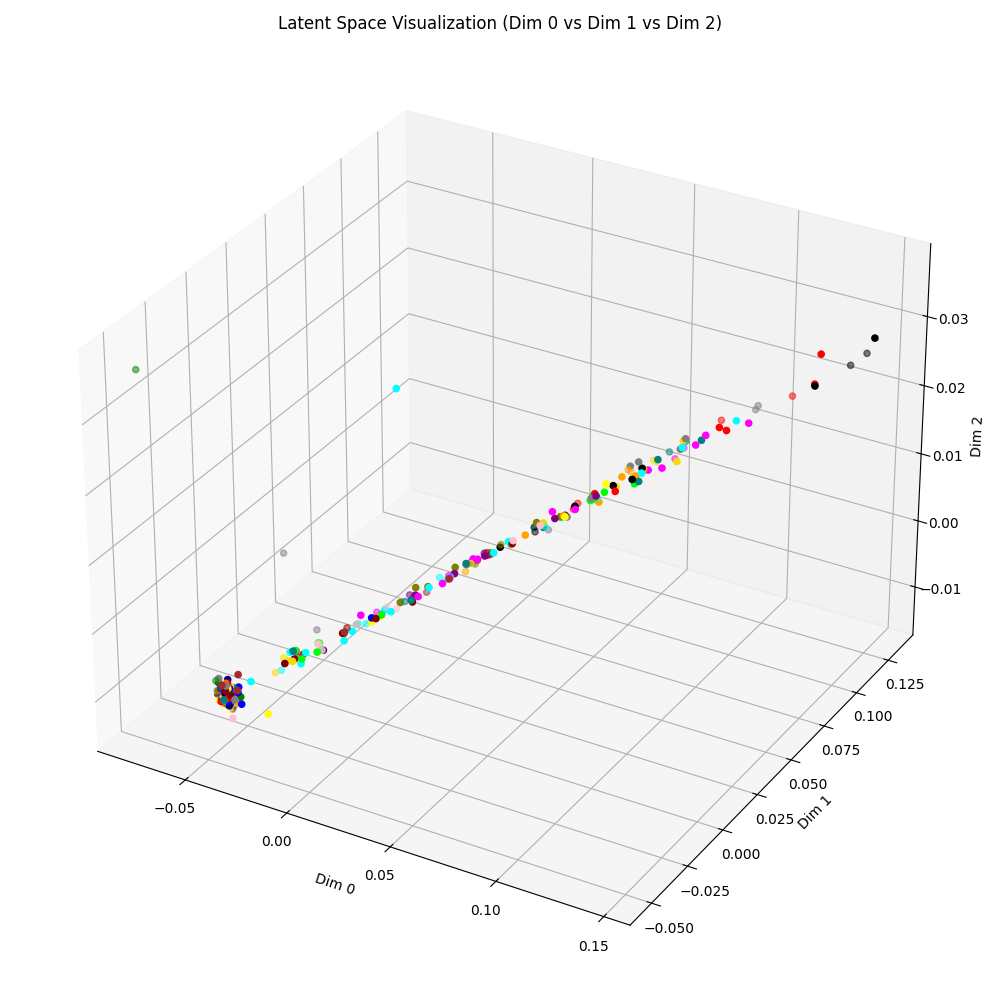
\includegraphics[width=\imgsize]{images/latent_space_viz_dataset_PigArtPressure_original.png} & 
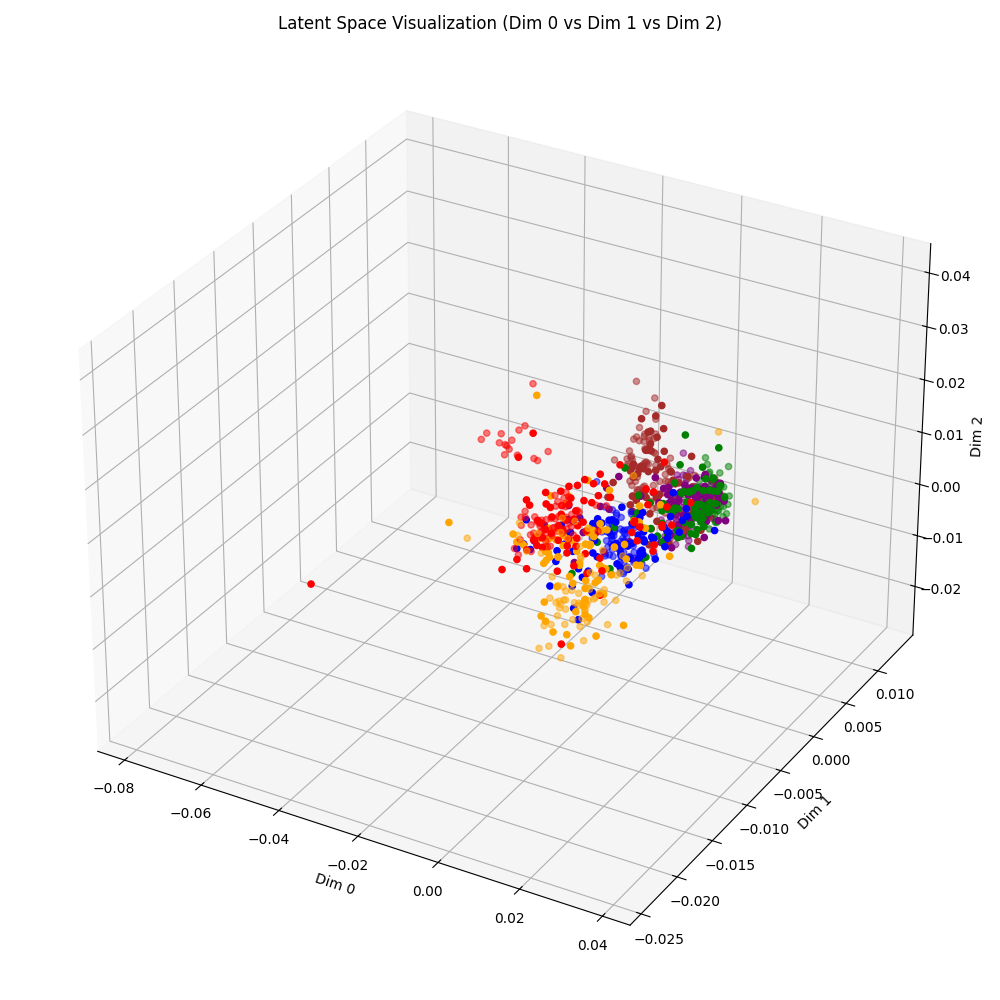
\includegraphics[width=\imgsize]{images/latent_space_viz_dataset_SemgHandMovementCh2_original.png} \\

Step 0 & 
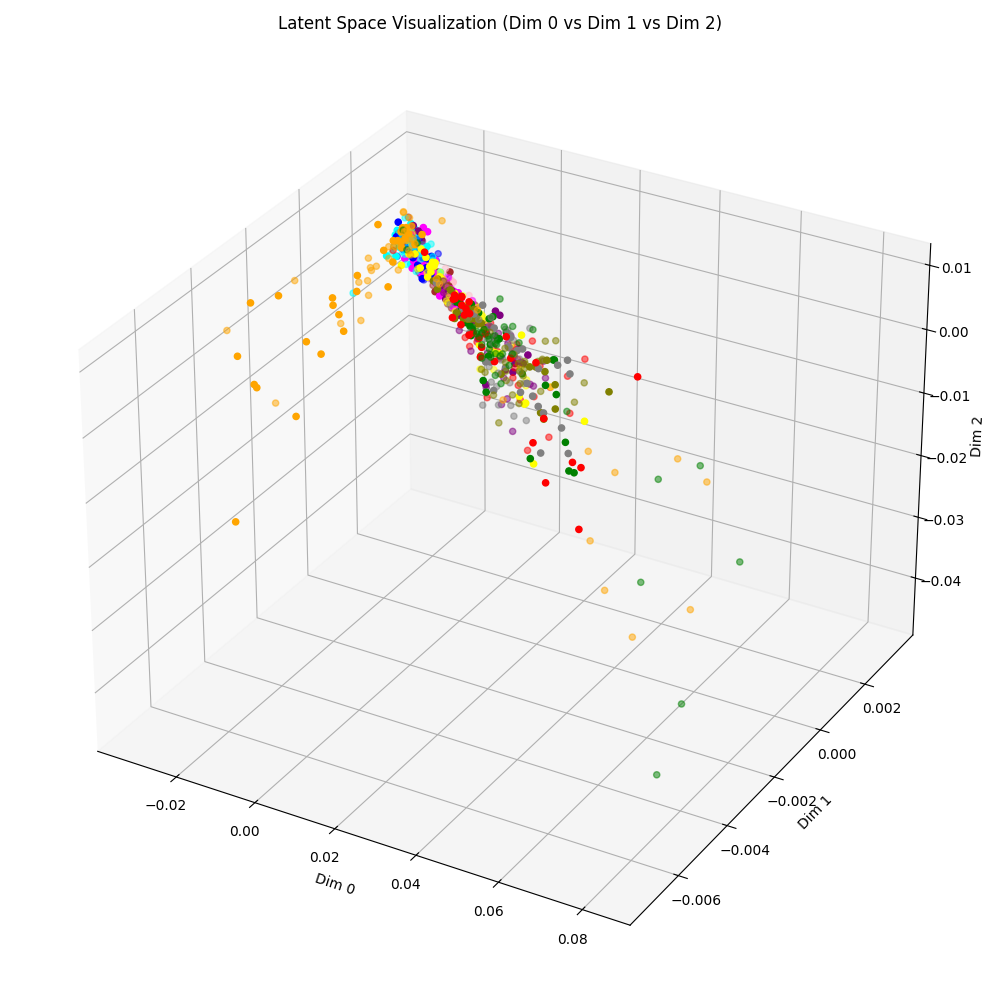
\includegraphics[width=\imgsize]{images/latent_space_viz_dataset_EOGVerticalSignal_before_augmented_step_0.png} & 
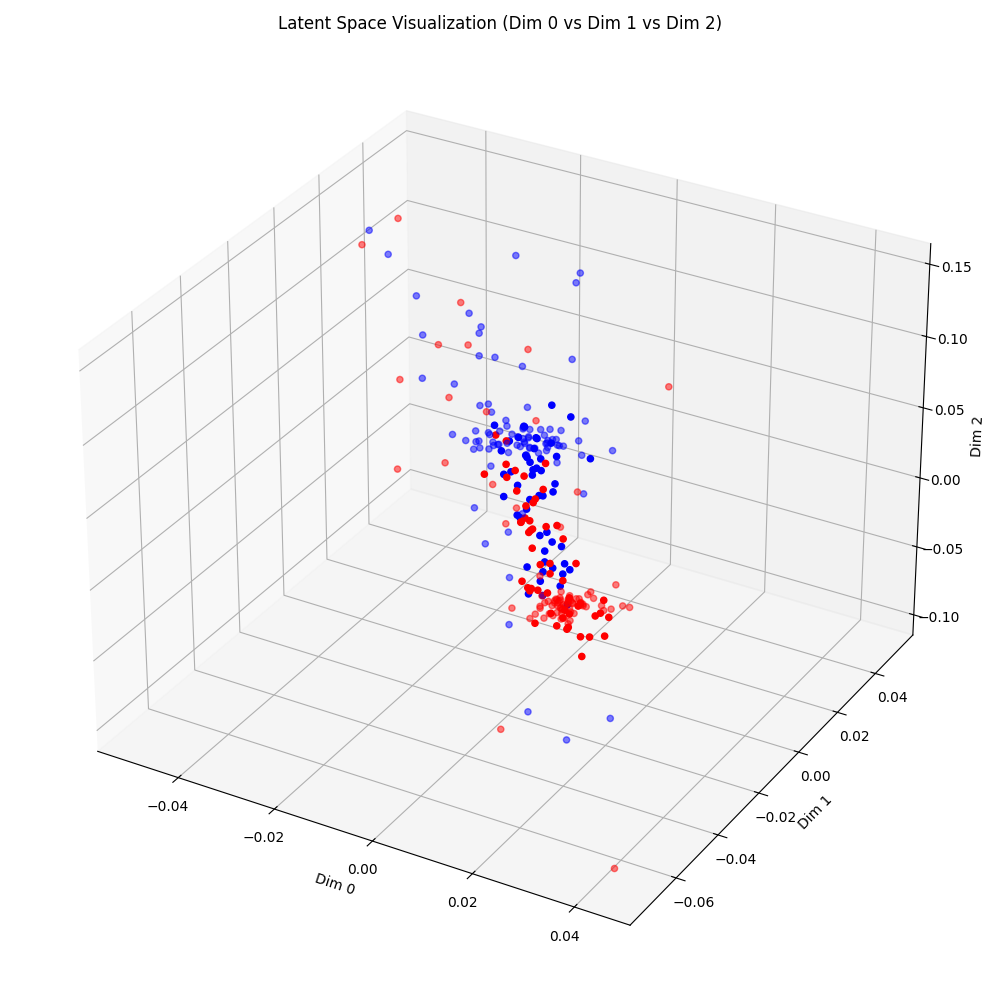
\includegraphics[width=\imgsize]{images/latent_space_viz_dataset_Ham_augmented_step_0.png} & 
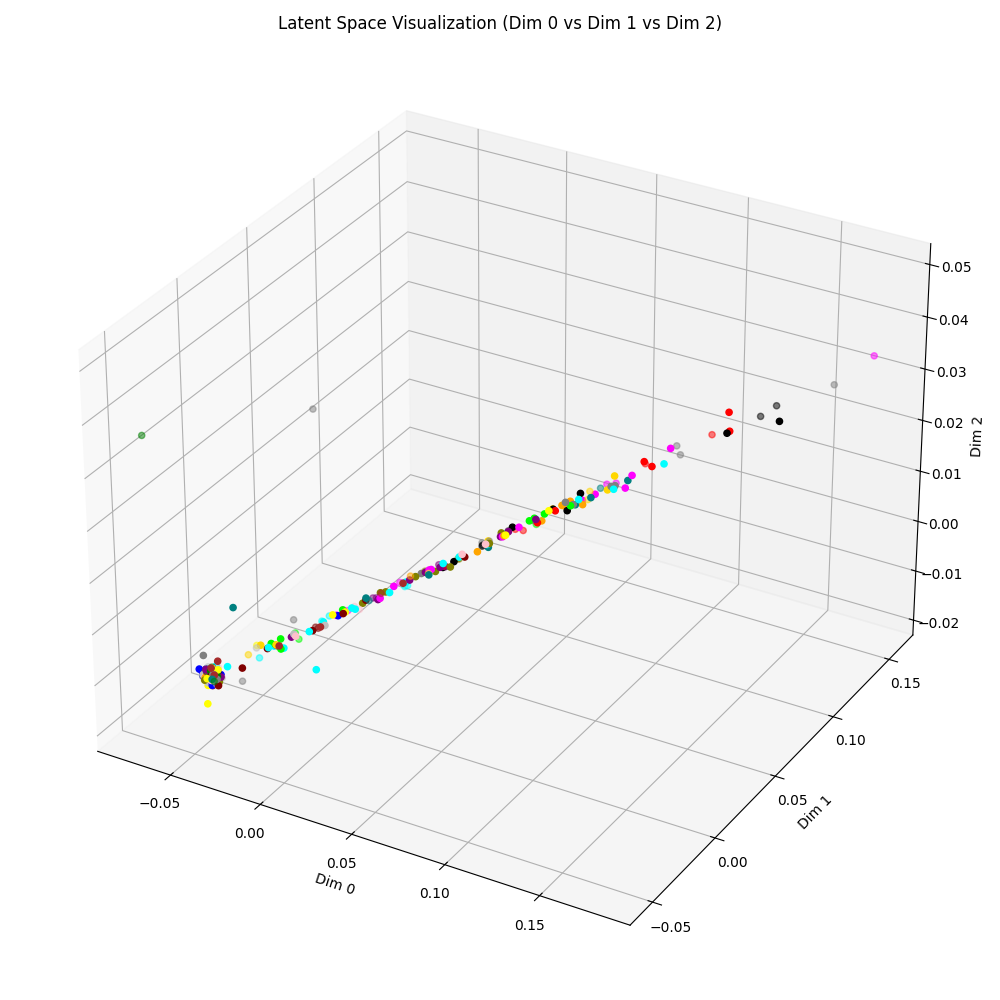
\includegraphics[width=\imgsize]{images/latent_space_viz_dataset_PigArtPressure_before_augmented_step_0.png} & 
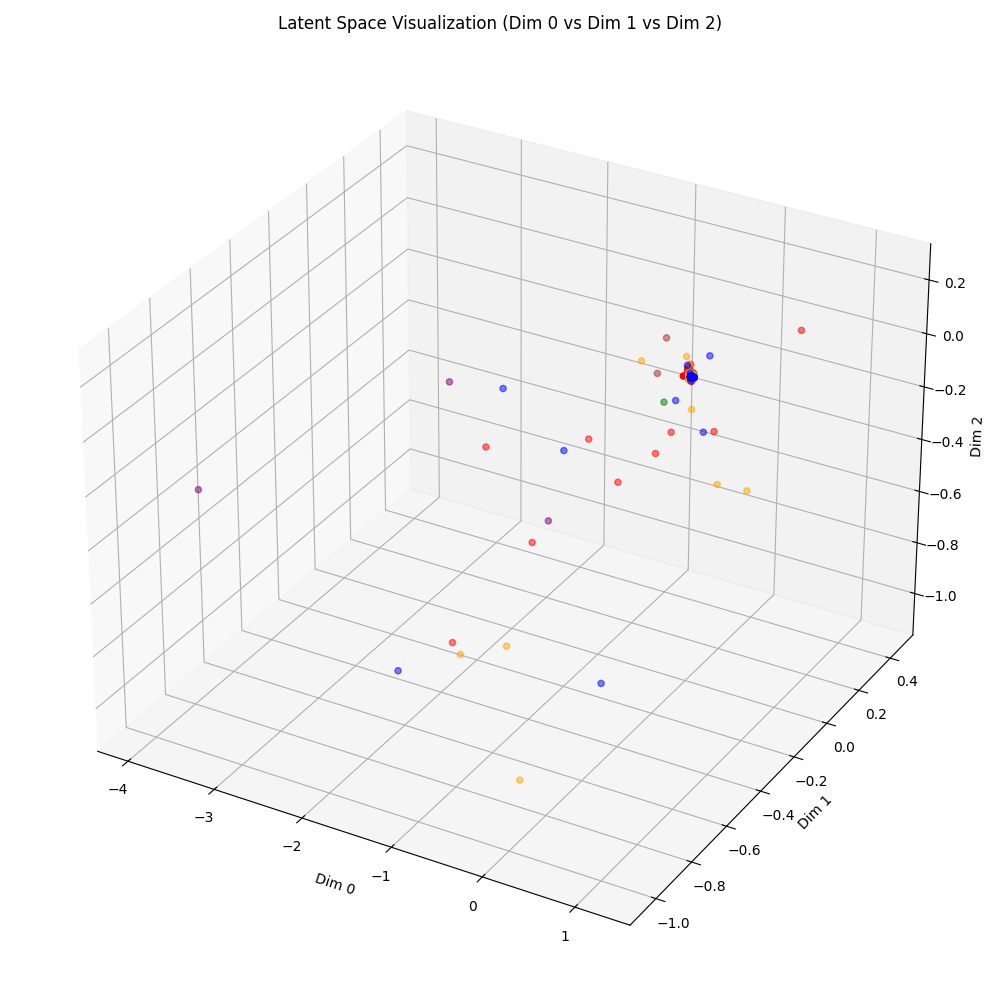
\includegraphics[width=\imgsize]{images/latent_space_viz_dataset_SemgHandMovementCh2_before_augmented_step_0.png} \\

Step 1 & 
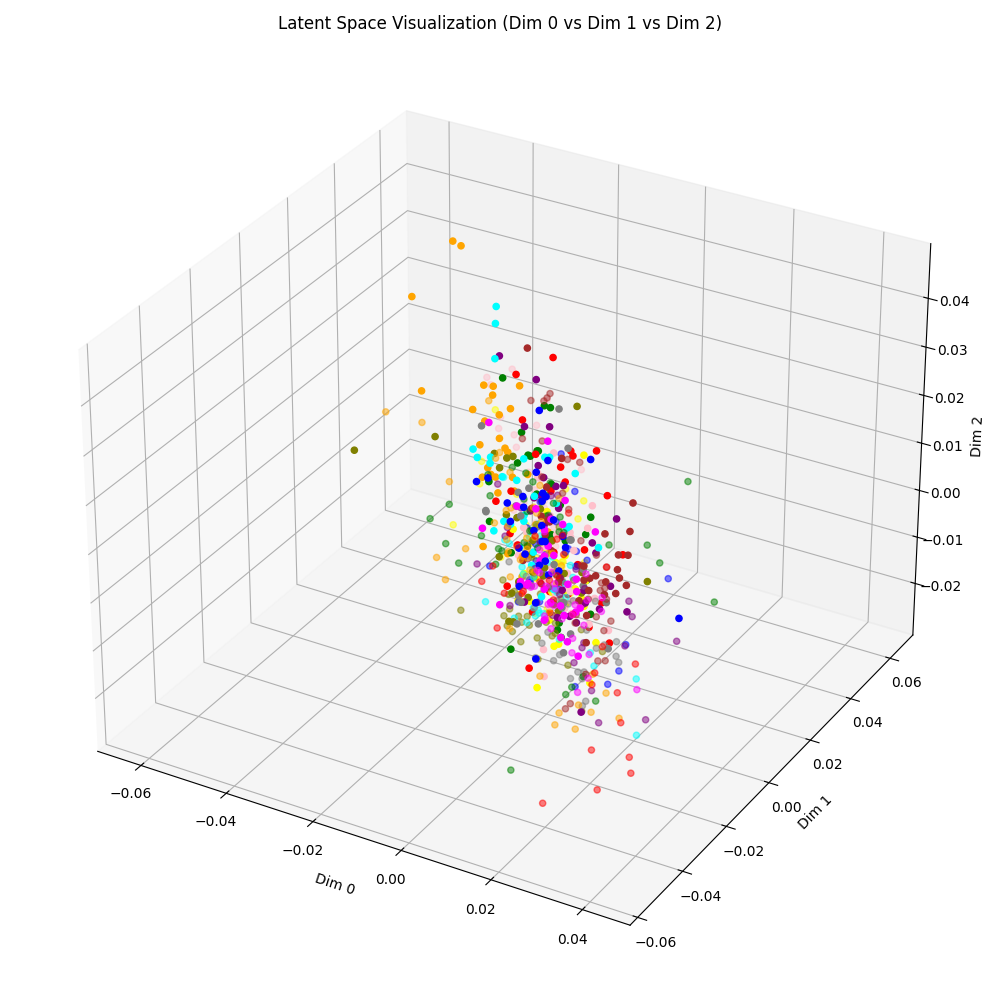
\includegraphics[width=\imgsize]{images/latent_space_viz_dataset_EOGVerticalSignal_augmented_step_1.png} & 
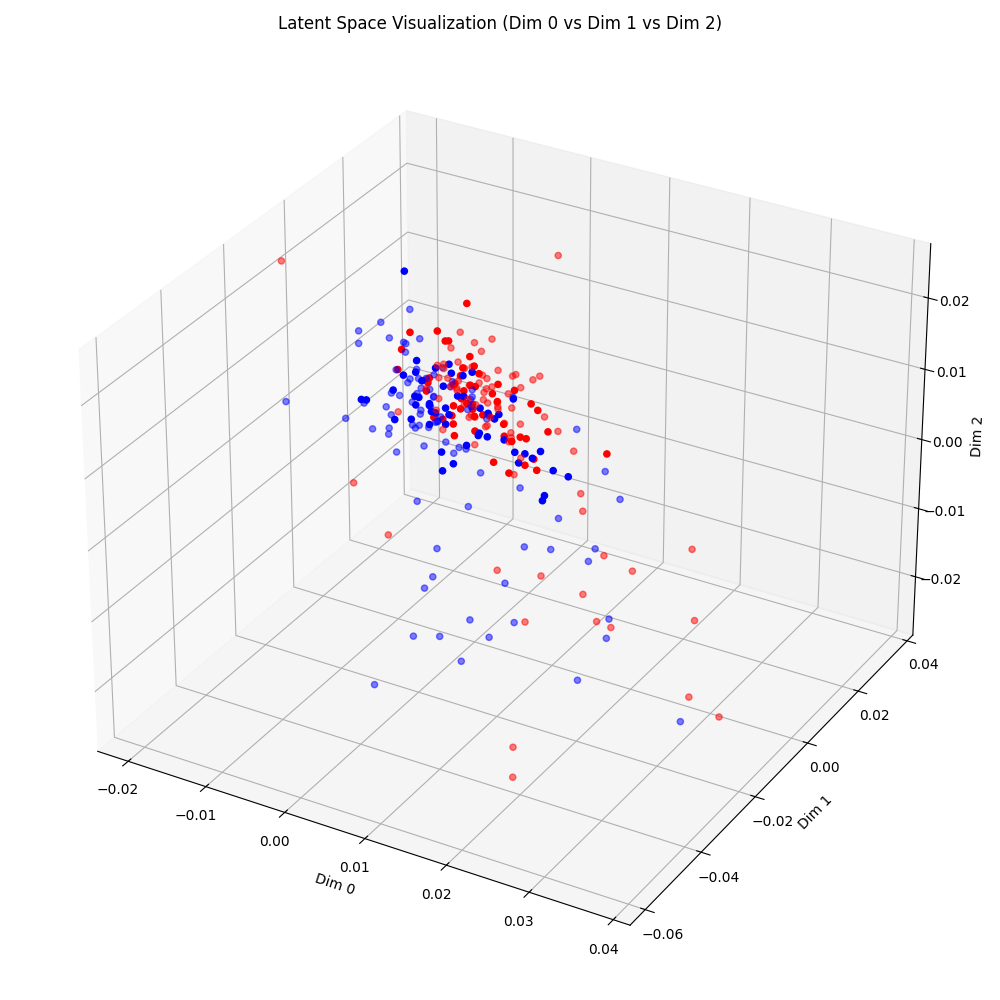
\includegraphics[width=\imgsize]{images/latent_space_viz_dataset_Ham_augmented_step_1.png} & 
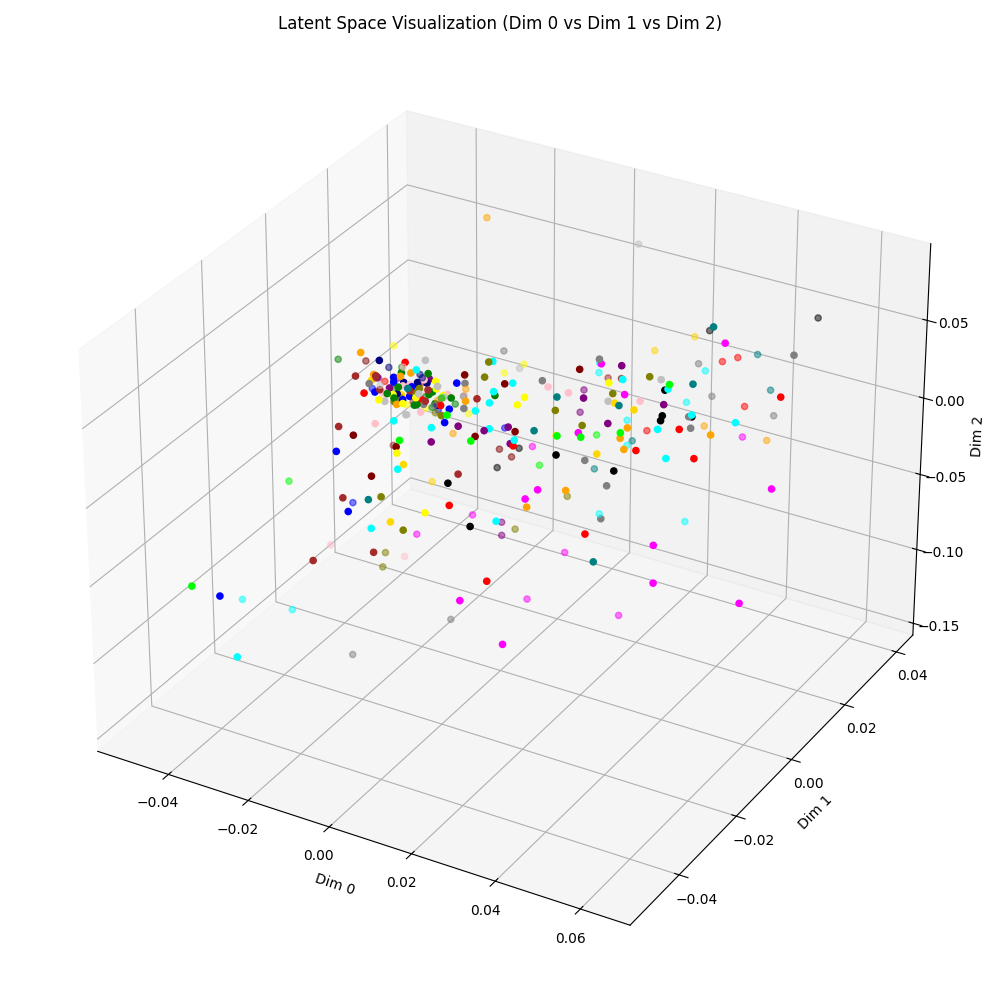
\includegraphics[width=\imgsize]{images/latent_space_viz_dataset_PigArtPressure_augmented_step_1.png} & 
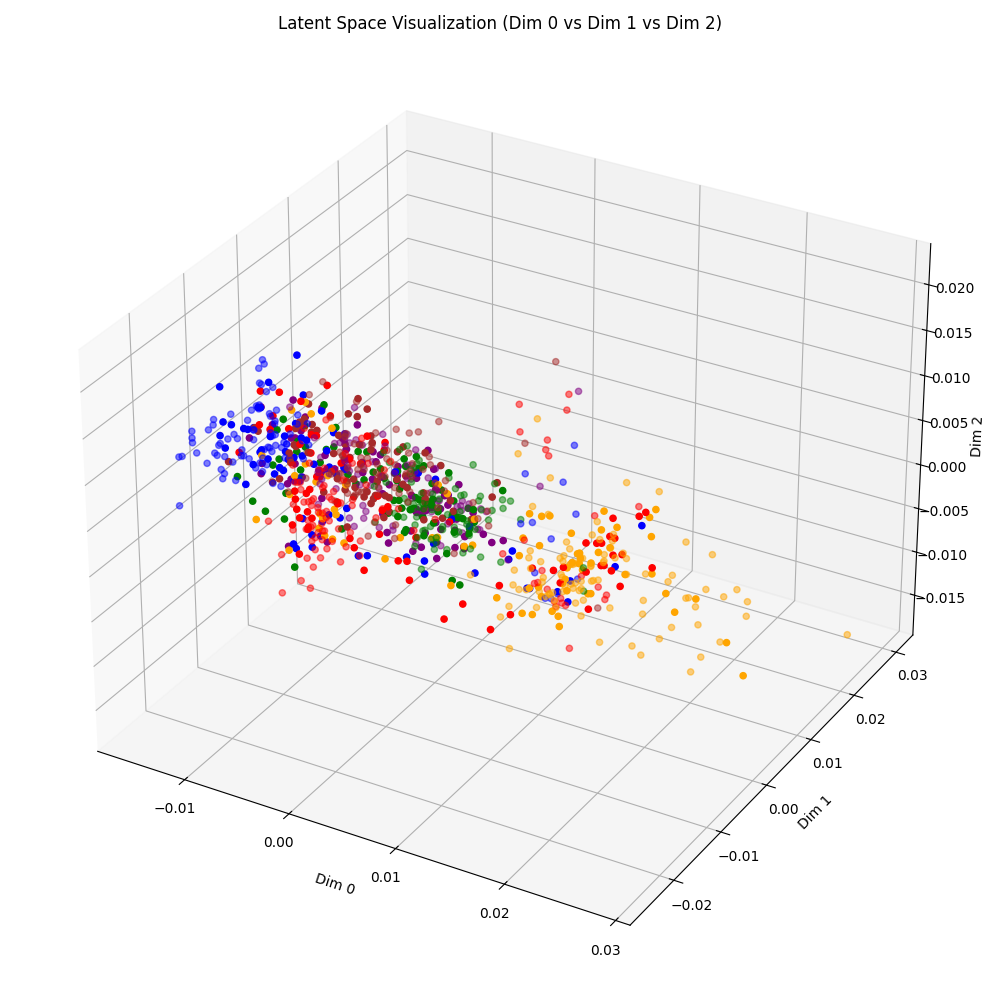
\includegraphics[width=\imgsize]{images/latent_space_viz_dataset_SemgHandMovementCh2_augmented_step_1.png} \\

Step 2 & 
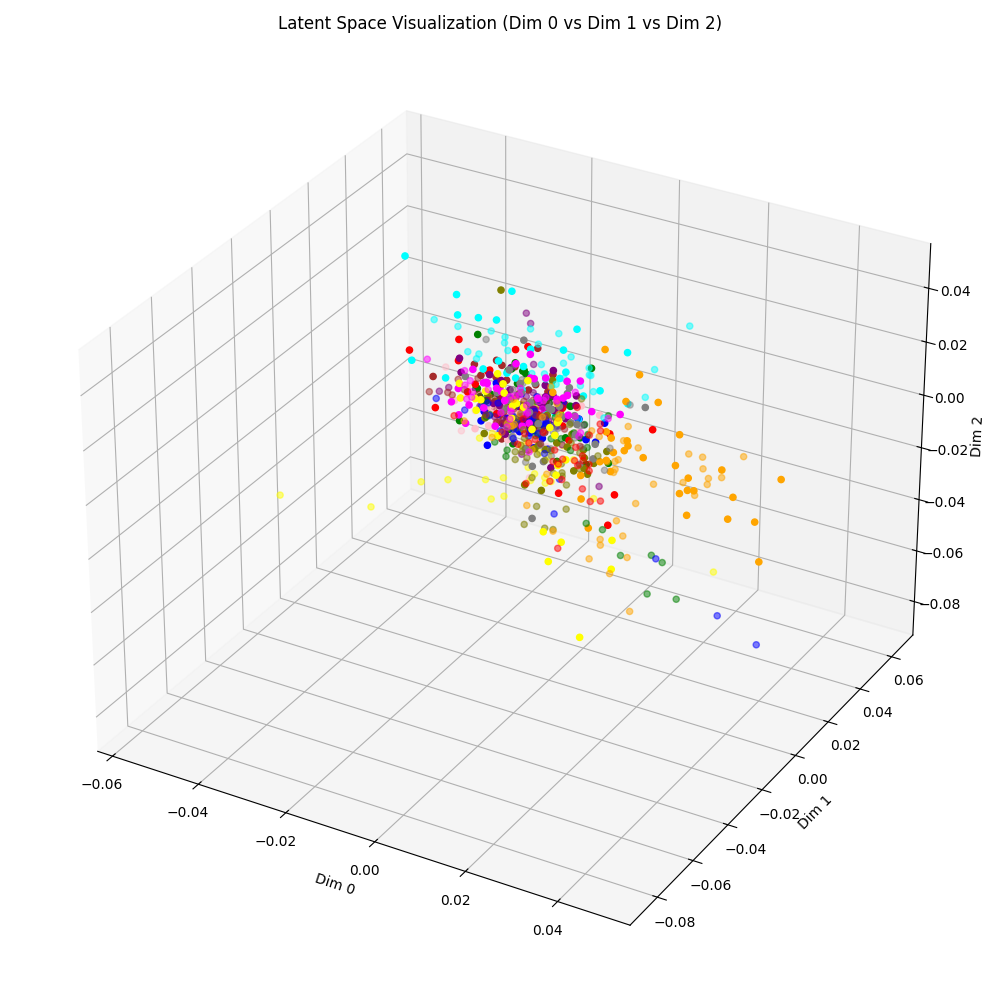
\includegraphics[width=\imgsize]{images/latent_space_viz_dataset_EOGVerticalSignal_augmented_step_2.png} & 
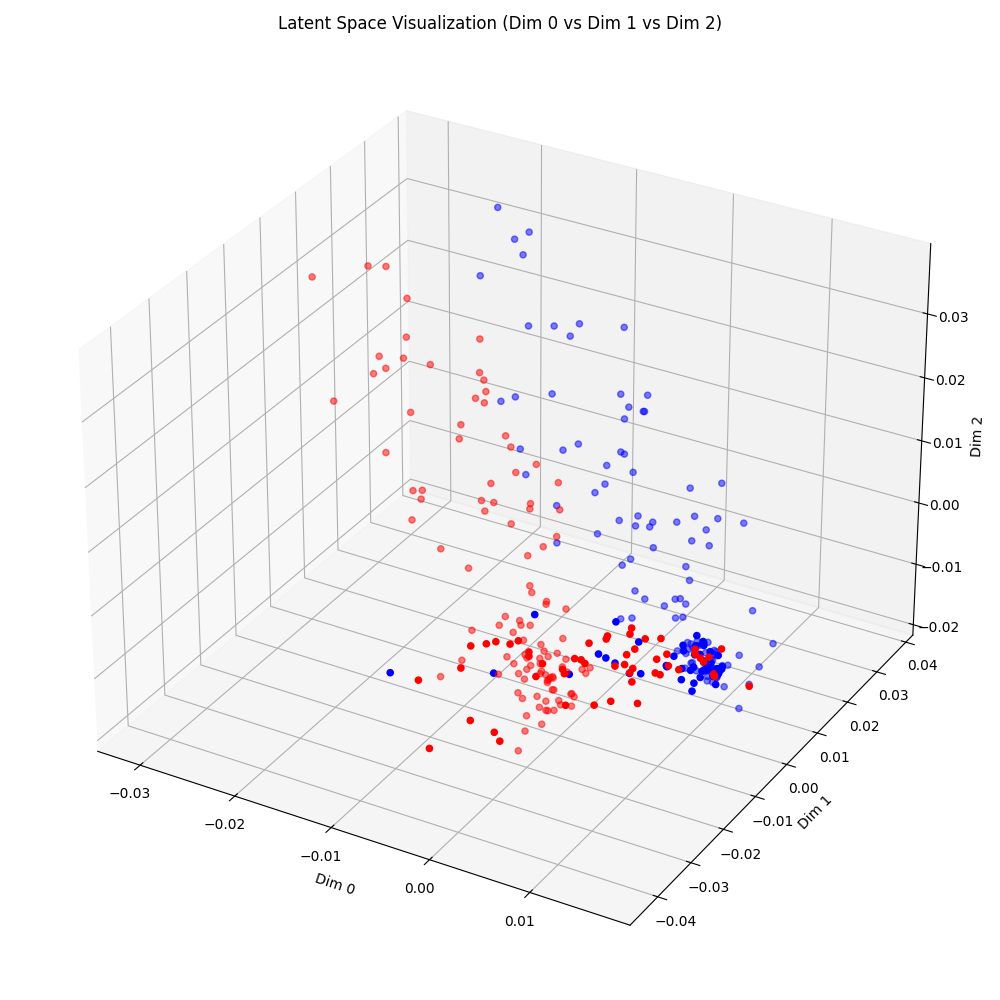
\includegraphics[width=\imgsize]{images/latent_space_viz_dataset_Ham_augmented_step_2.png} & 
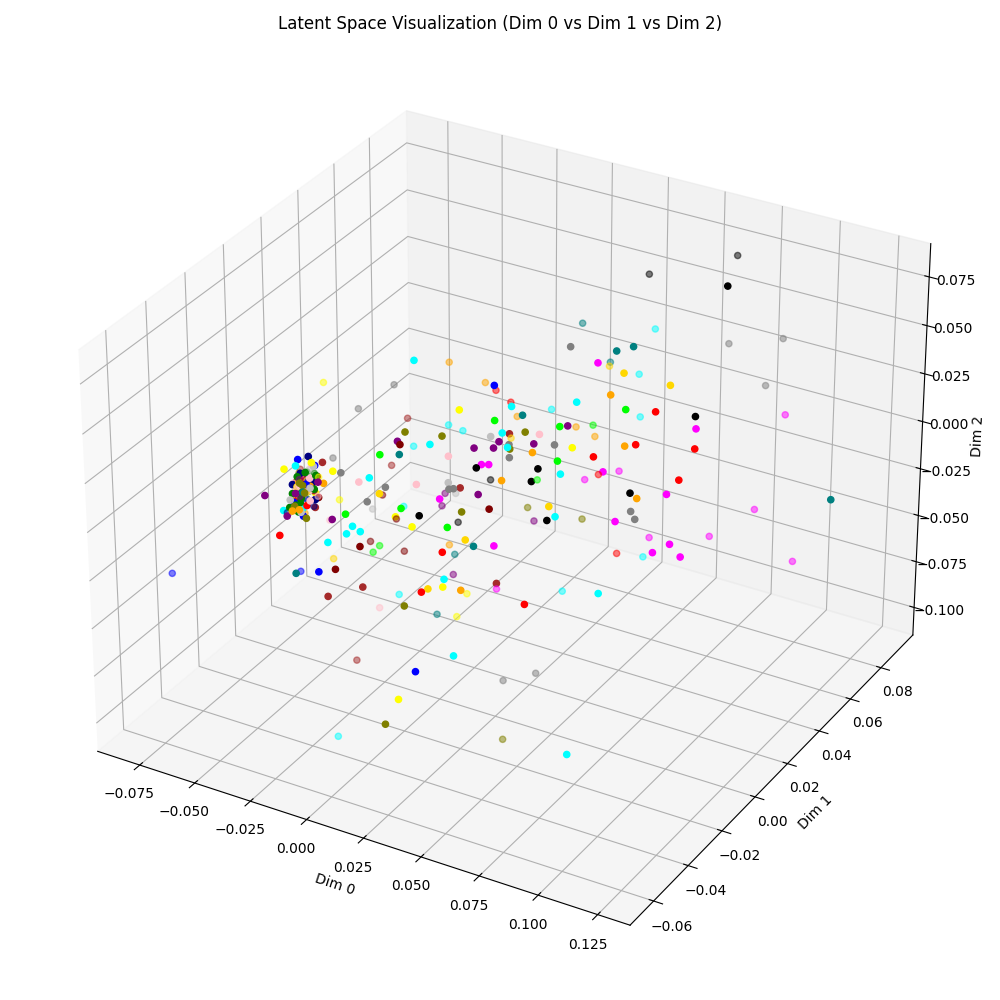
\includegraphics[width=\imgsize]{images/latent_space_viz_dataset_PigArtPressure_augmented_step_2.png} & 
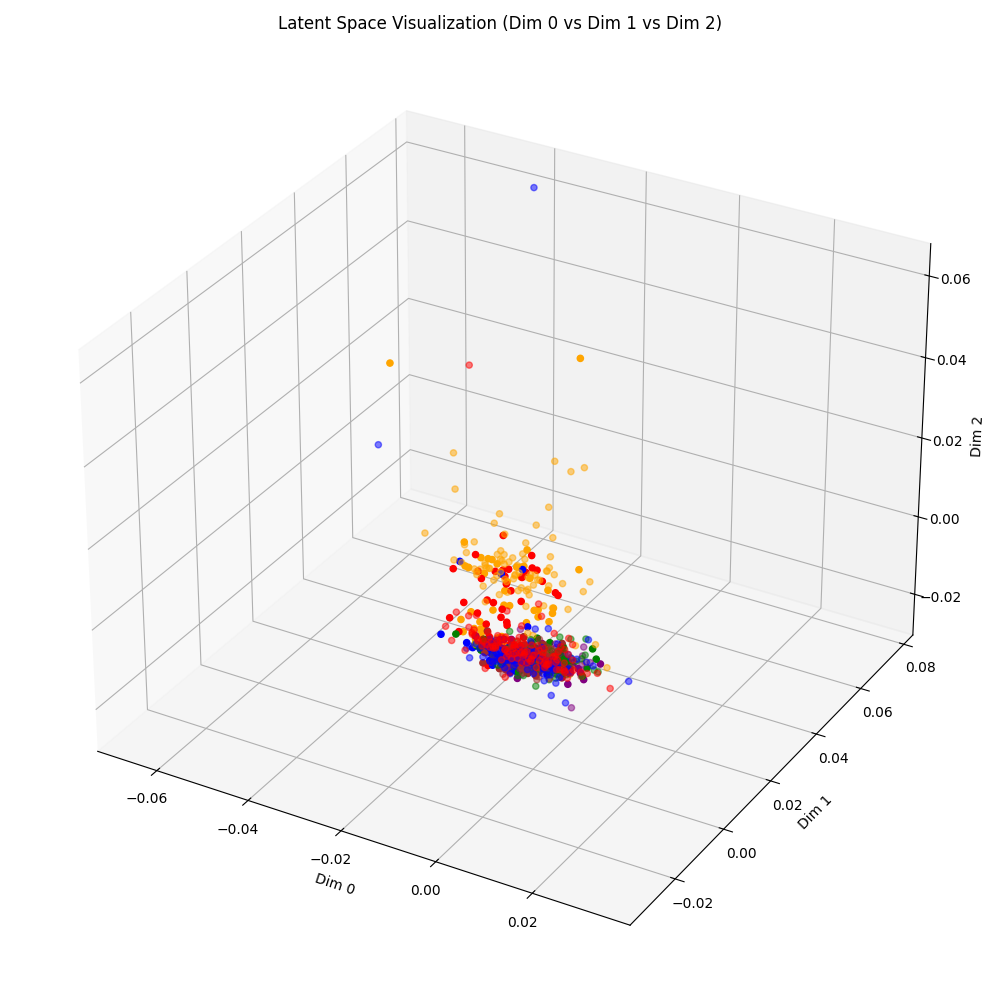
\includegraphics[width=\imgsize]{images/latent_space_viz_dataset_SemgHandMovementCh2_augmented_step_2.png} \\

Step 3 & 
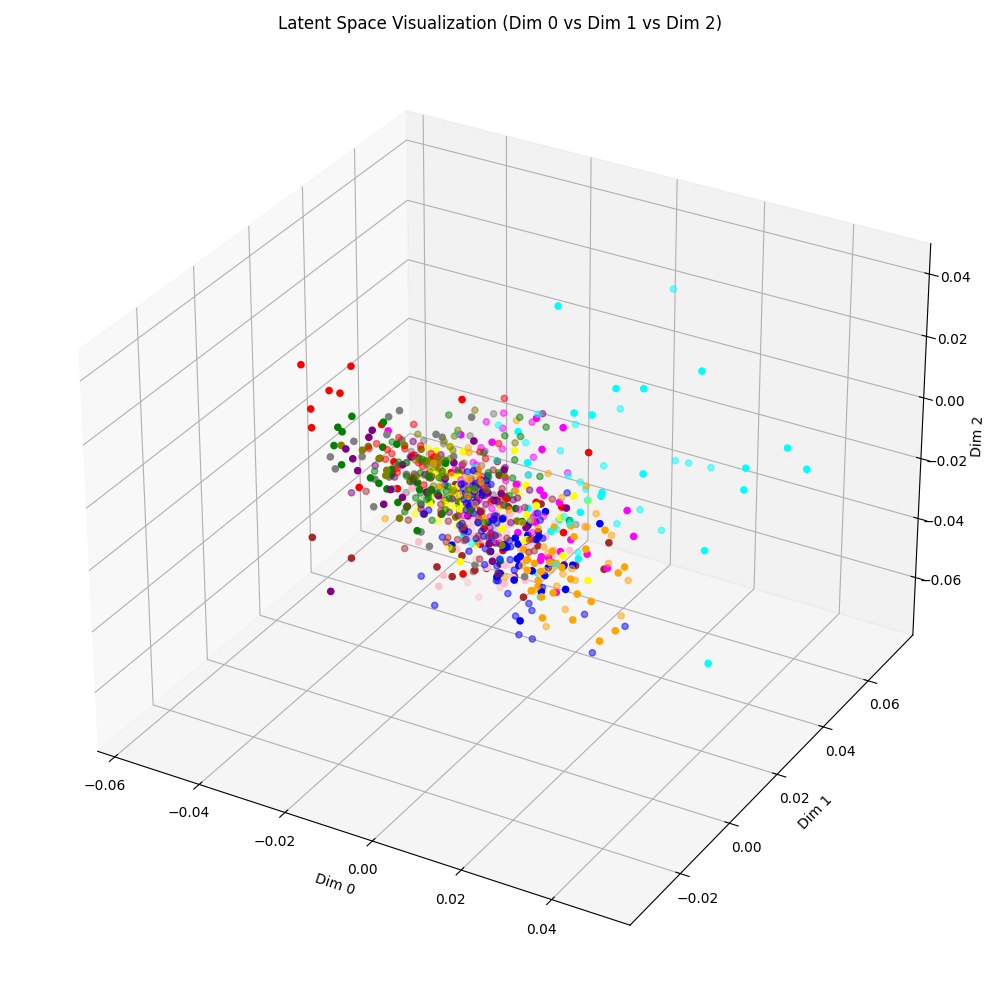
\includegraphics[width=\imgsize]{images/latent_space_viz_dataset_EOGVerticalSignal_augmented_step_3.png} & 
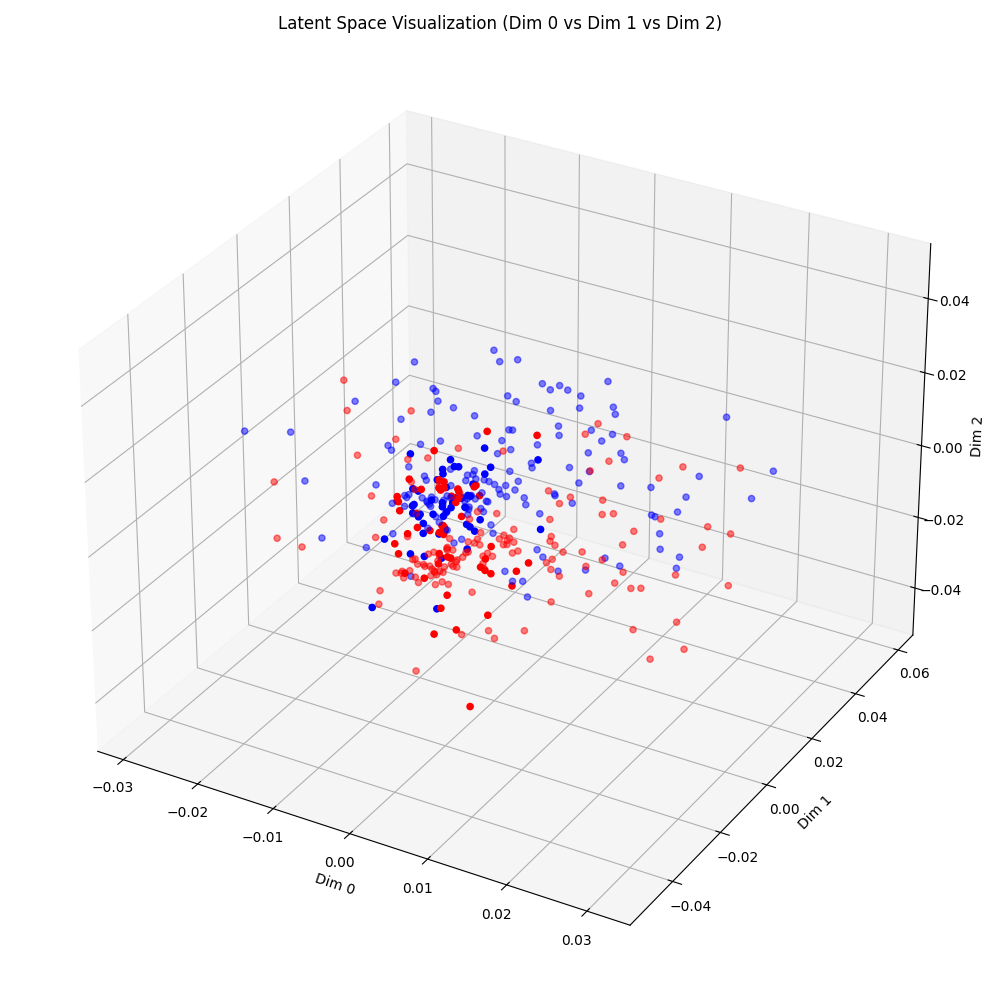
\includegraphics[width=\imgsize]{images/latent_space_viz_dataset_Ham_augmented_step_3.png} & 
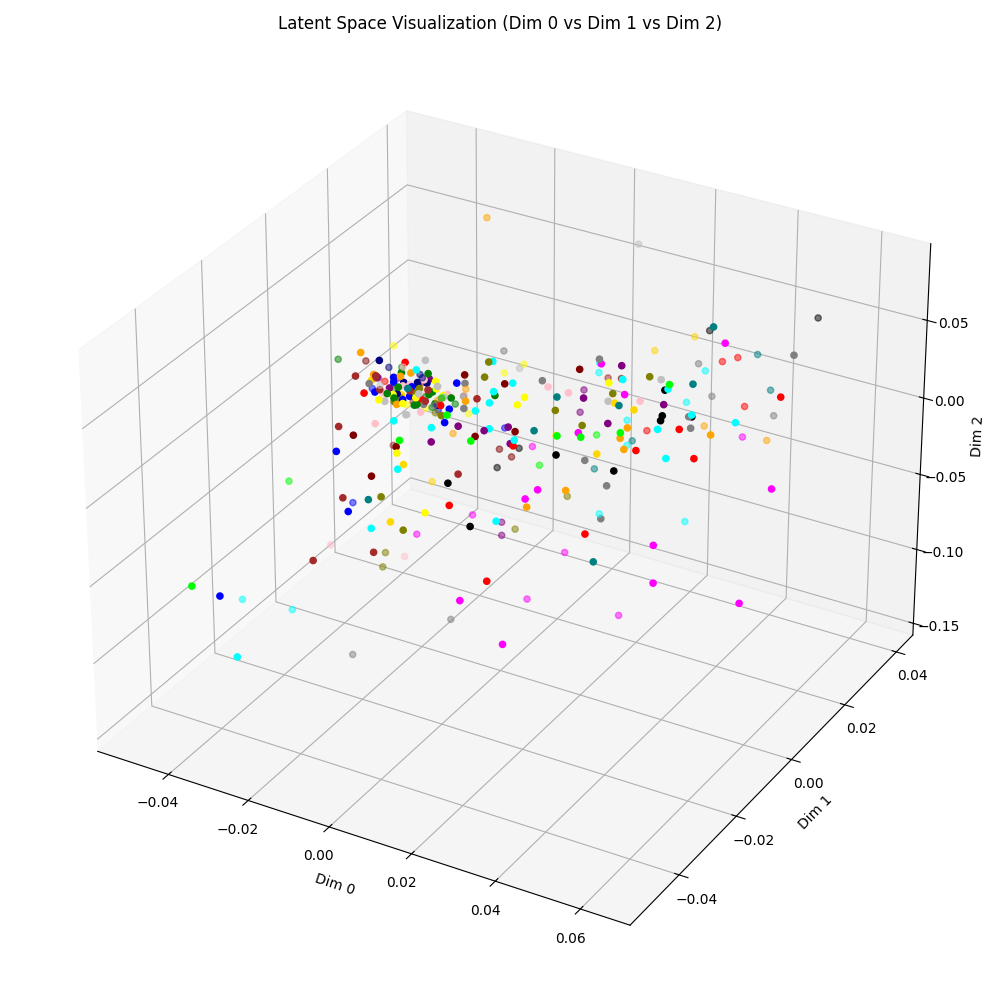
\includegraphics[width=\imgsize]{images/latent_space_viz_dataset_PigArtPressure_augmented_step_1.png} & 
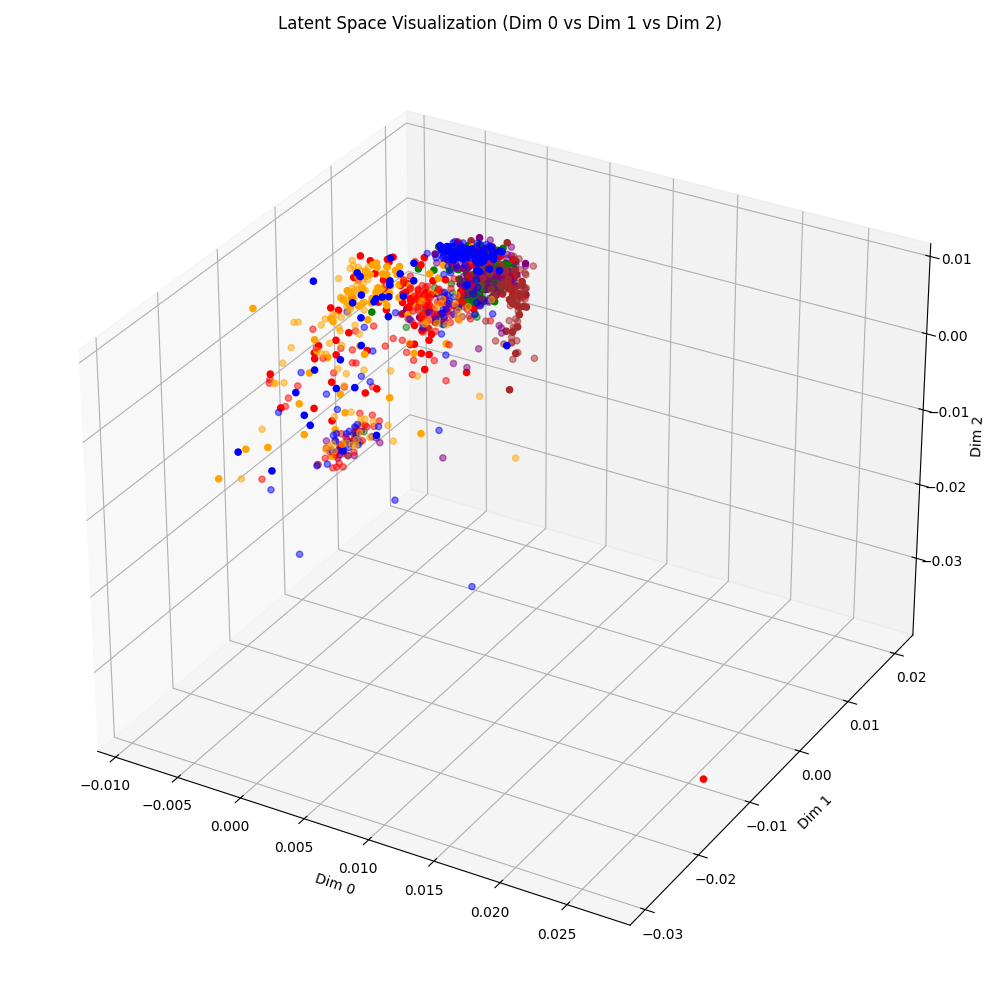
\includegraphics[width=\imgsize]{images/latent_space_viz_dataset_SemgHandMovementCh2_augmented_step_3.png}

 \\ 

Step 4 & 
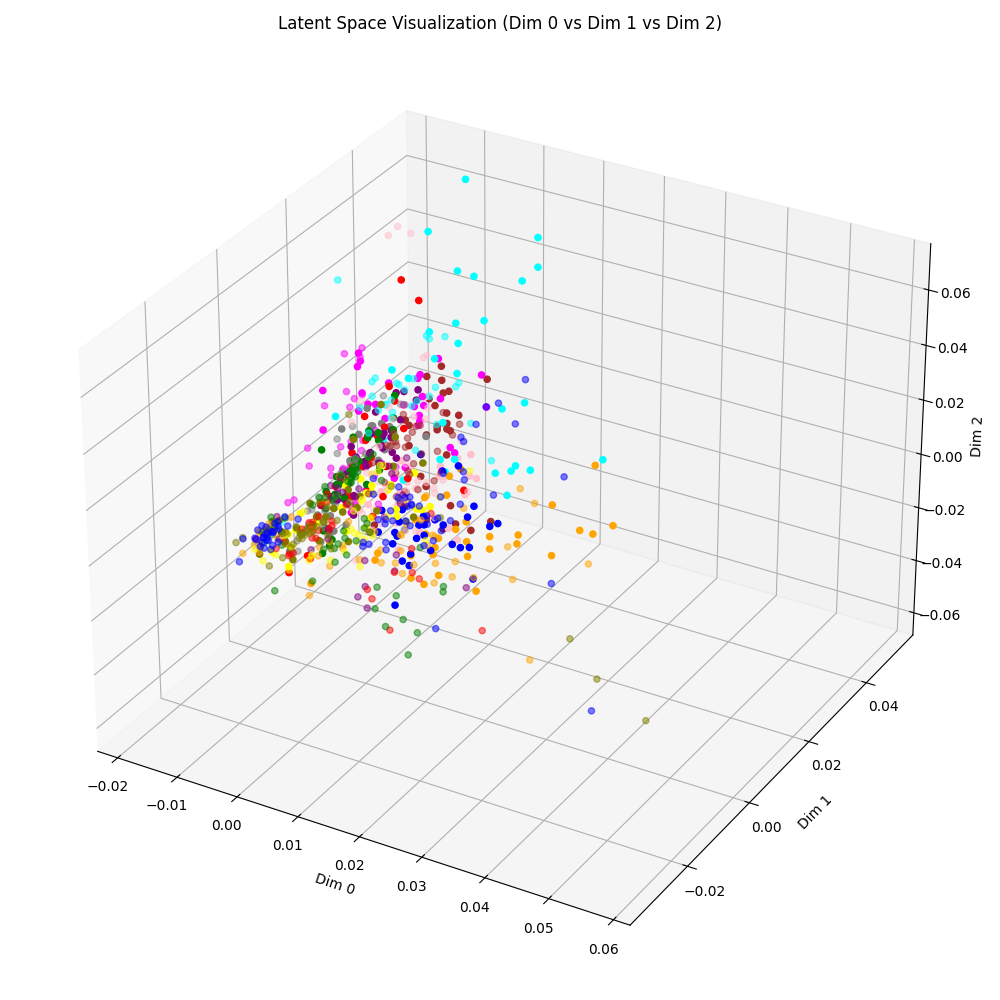
\includegraphics[width=\imgsize]{images/latent_space_viz_dataset_EOGVerticalSignal_augmented_step_4.png} & 
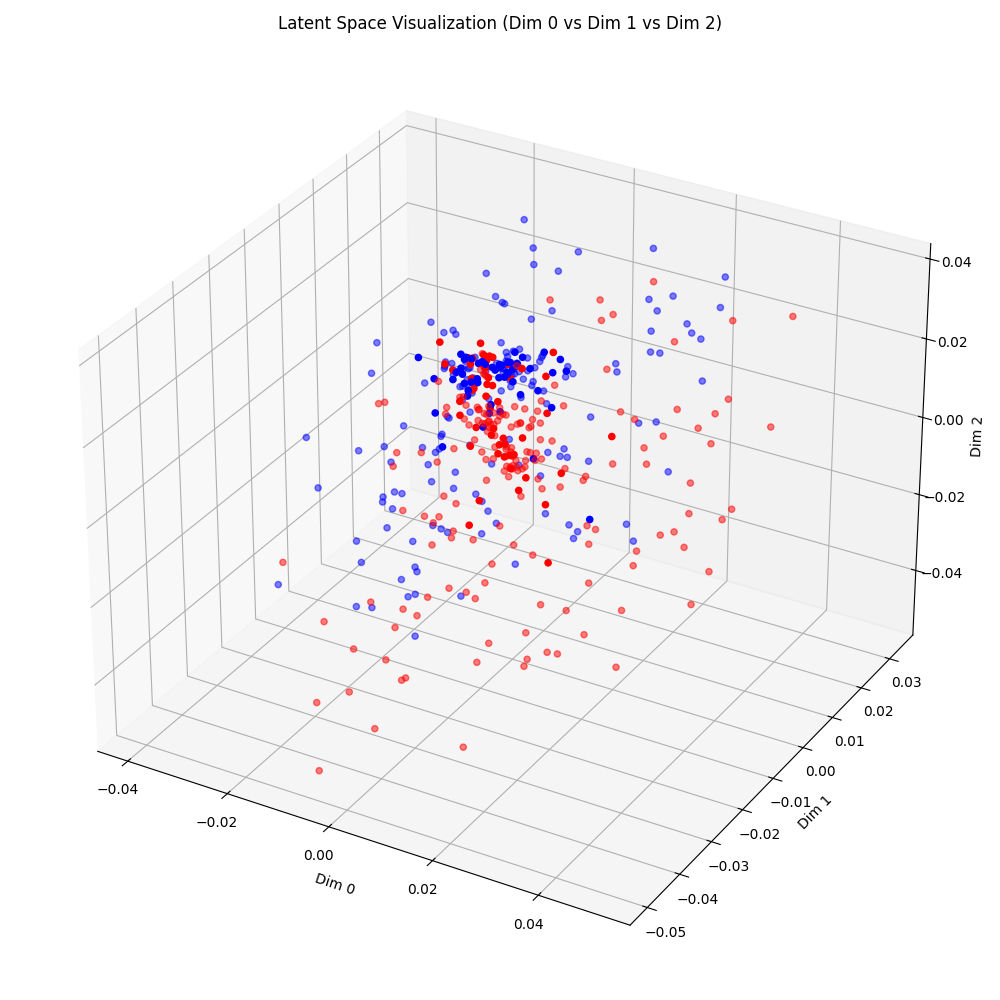
\includegraphics[width=\imgsize]{images/latent_space_viz_dataset_Ham_augmented_step_4.png} &
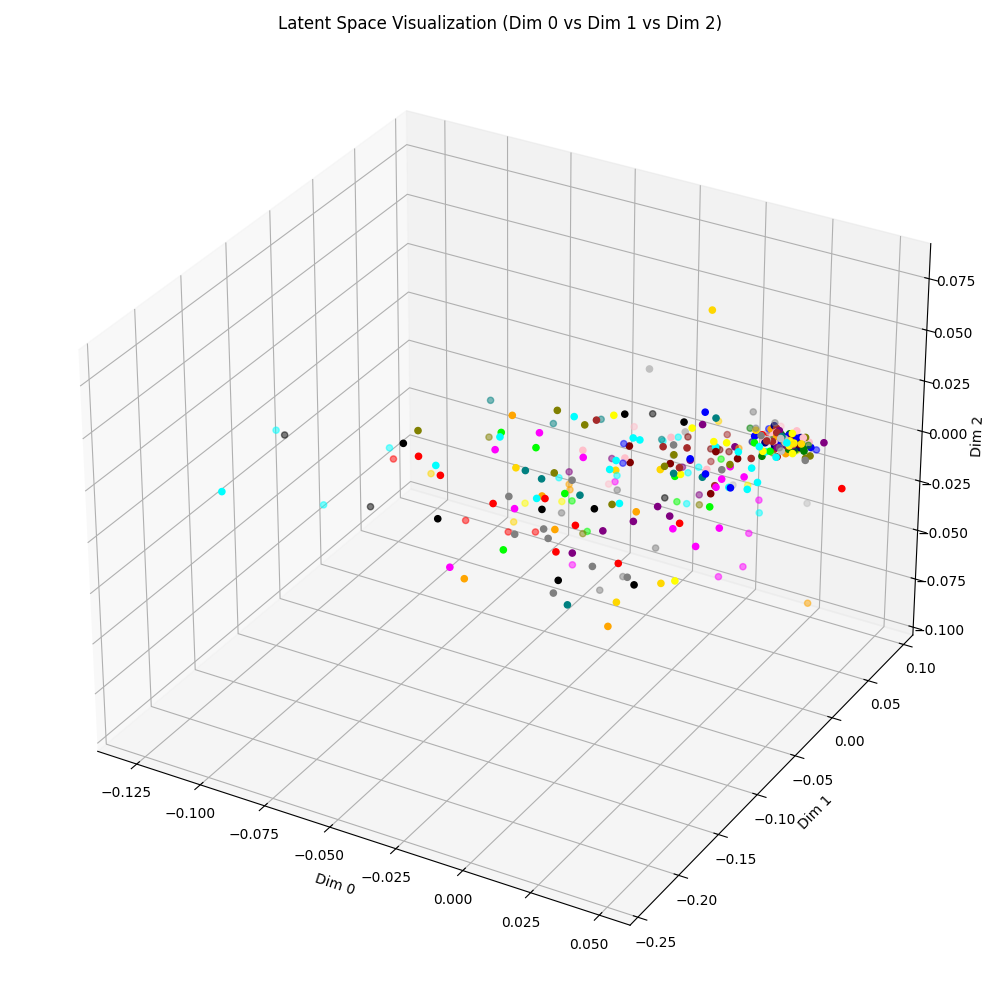
\includegraphics[width=\imgsize]{images/latent_space_viz_dataset_PigArtPressure_augmented_step_4.png} & 
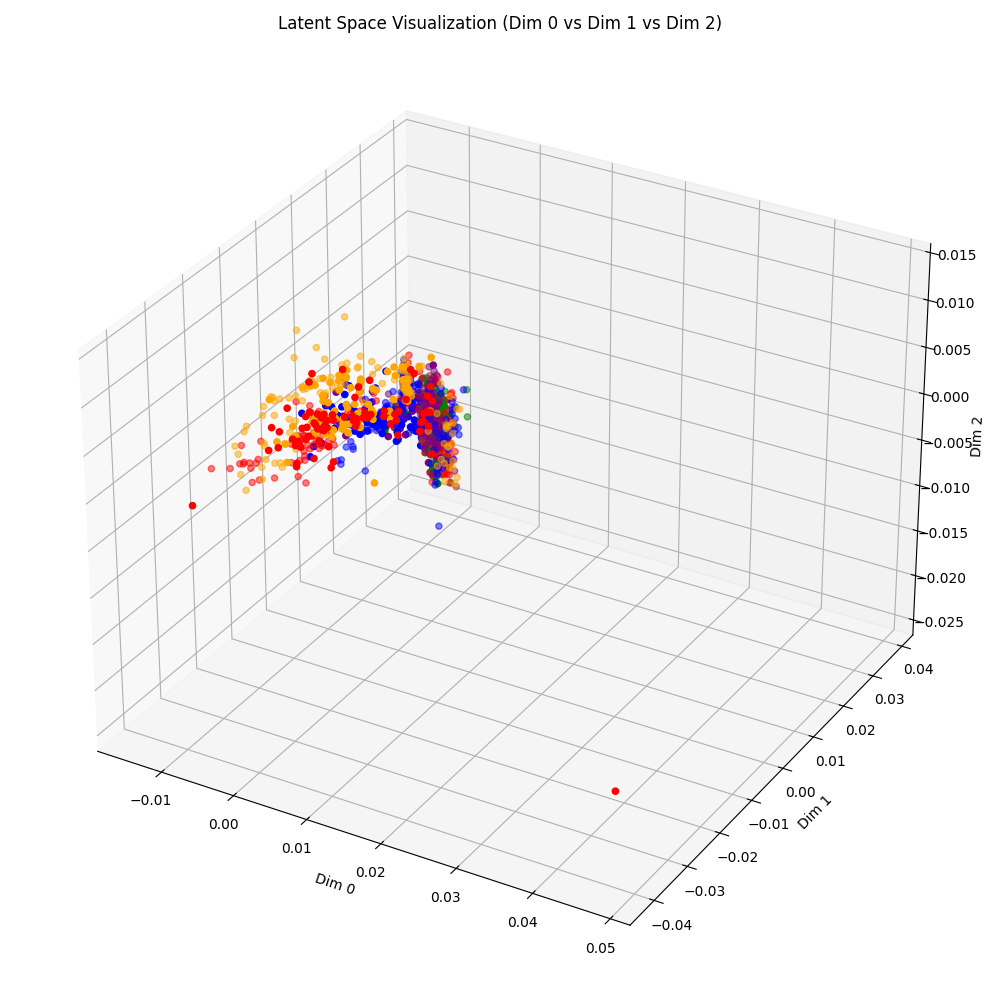
\includegraphics[width=\imgsize]{images/latent_space_viz_dataset_SemgHandMovementCh2_augmented_step_4.png}

\\ 

Step 5 & 
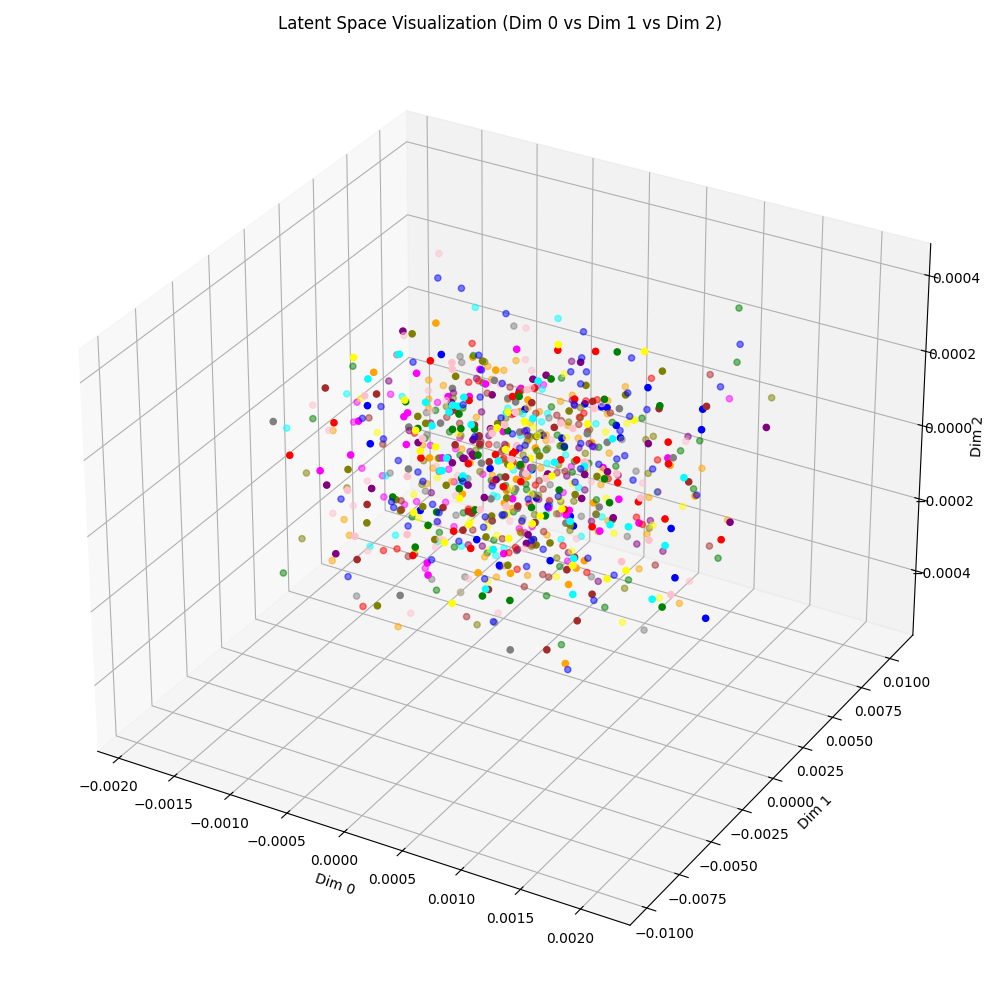
\includegraphics[width=\imgsize]{images/latent_space_viz_dataset_EOGVerticalSignal_augmented_step_5.png} & 
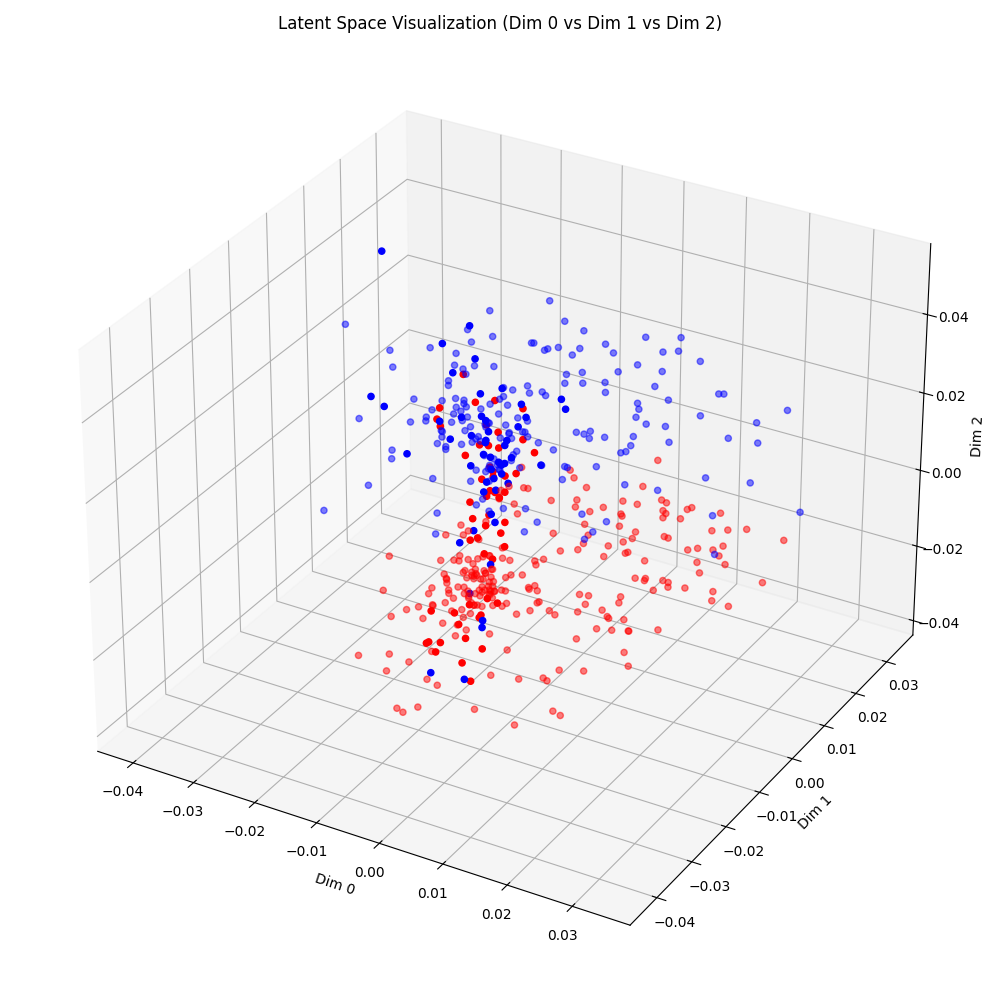
\includegraphics[width=\imgsize]{images/latent_space_viz_dataset_Ham_augmented_step_5.png} &
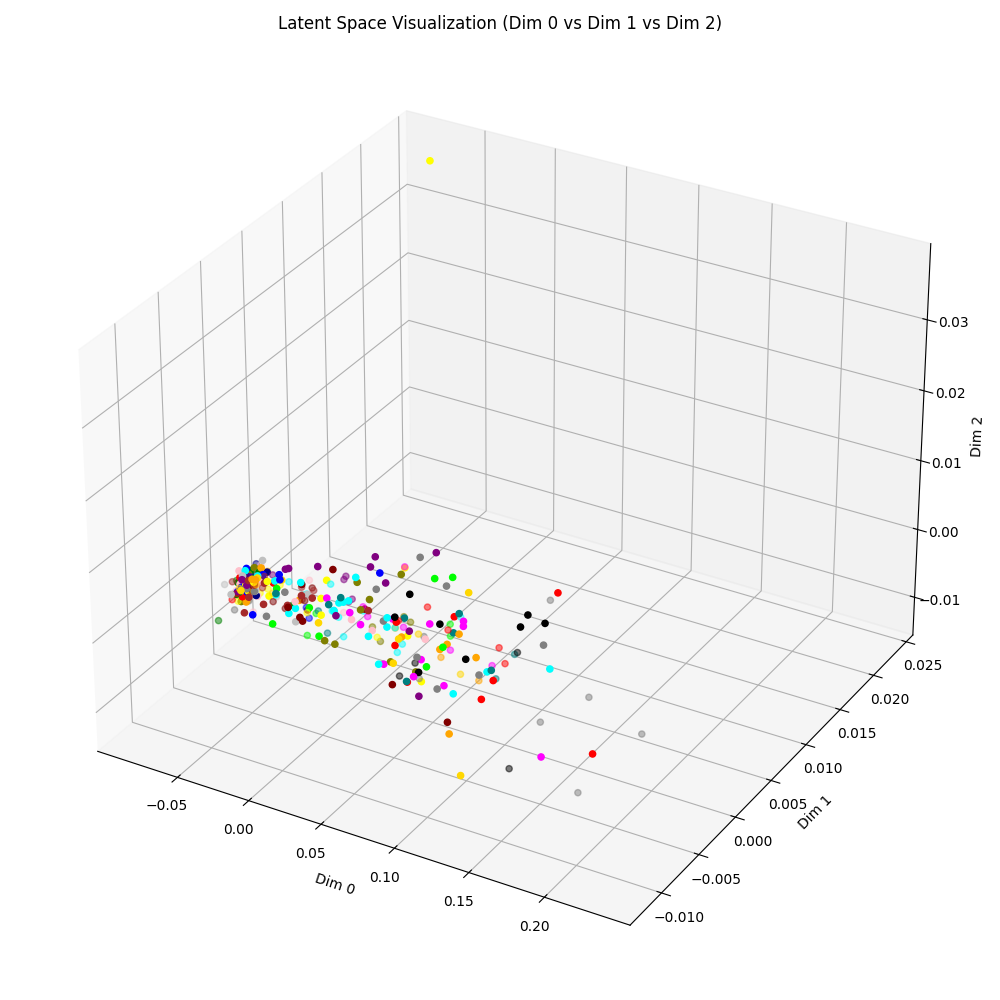
\includegraphics[width=\imgsize]{images/latent_space_viz_dataset_PigArtPressure_augmented_step_5.png} & 
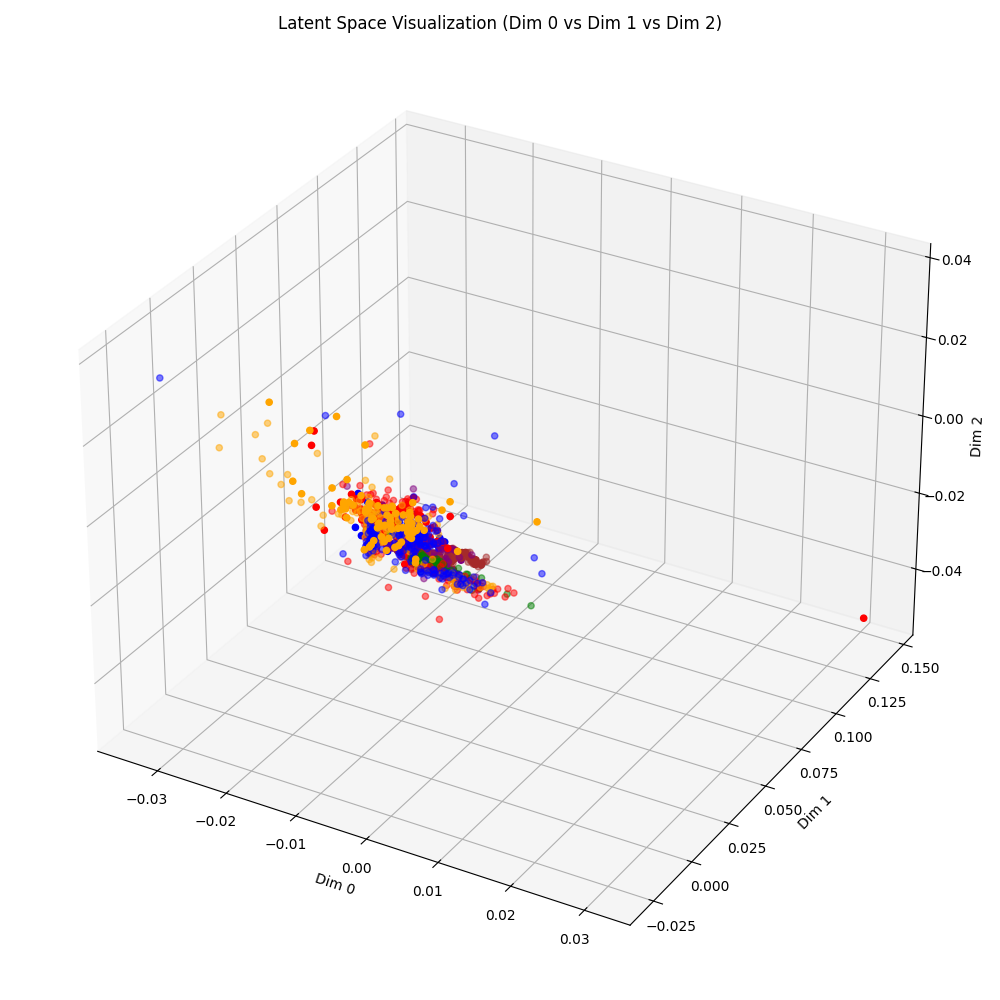
\includegraphics[width=\imgsize]{images/latent_space_viz_dataset_SemgHandMovementCh2_augmented_step_5.png}\\ 
\bottomrule
\end{tabular}
%\caption{Latent Space Evolution: EOGVerticalSignal, Ham, PigArtPressure, SemgHandMovementCh2}
\end{table*}

\newpage

\begin{table*}[h!]
\centering
\begin{tabular}{ccc}
\toprule
\bf Step & \bf UMD & \bf Worms \\ 
\midrule
Original & 
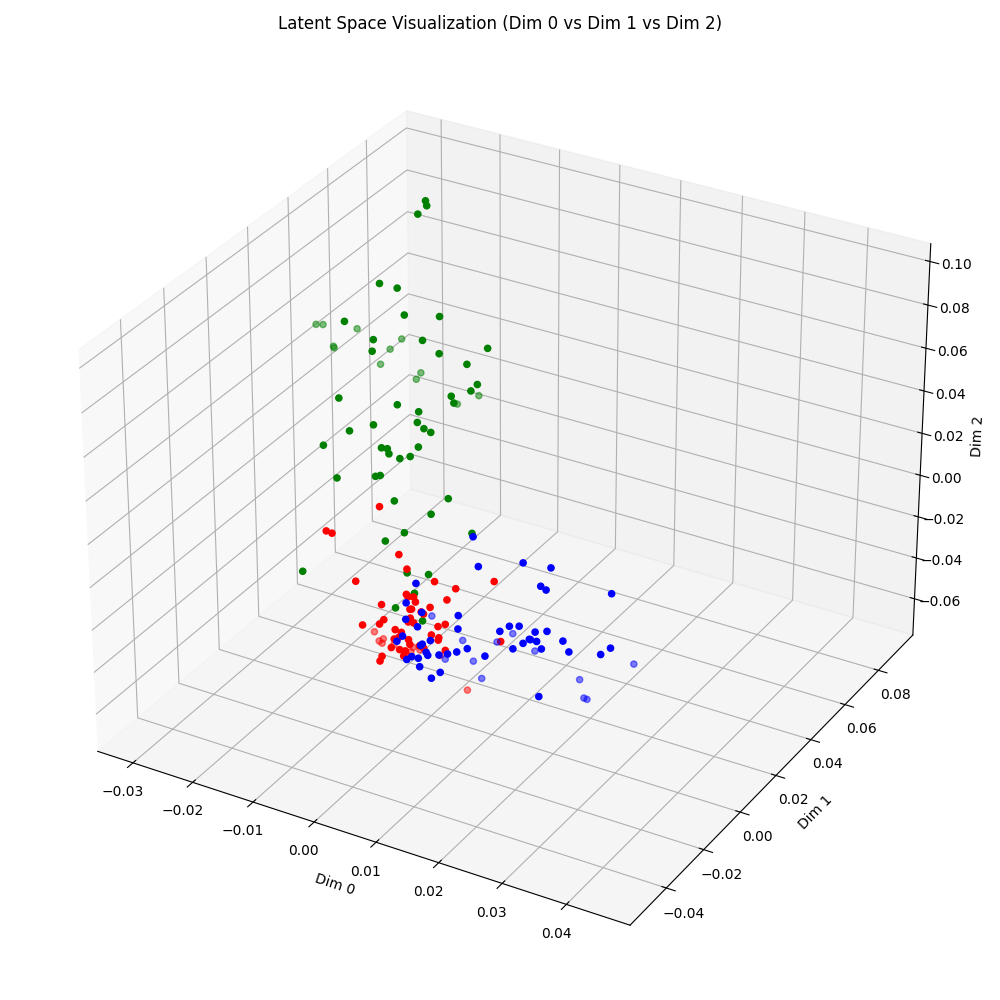
\includegraphics[width=\imgsize]{images/latent_space_viz_dataset_UMD.png} & 
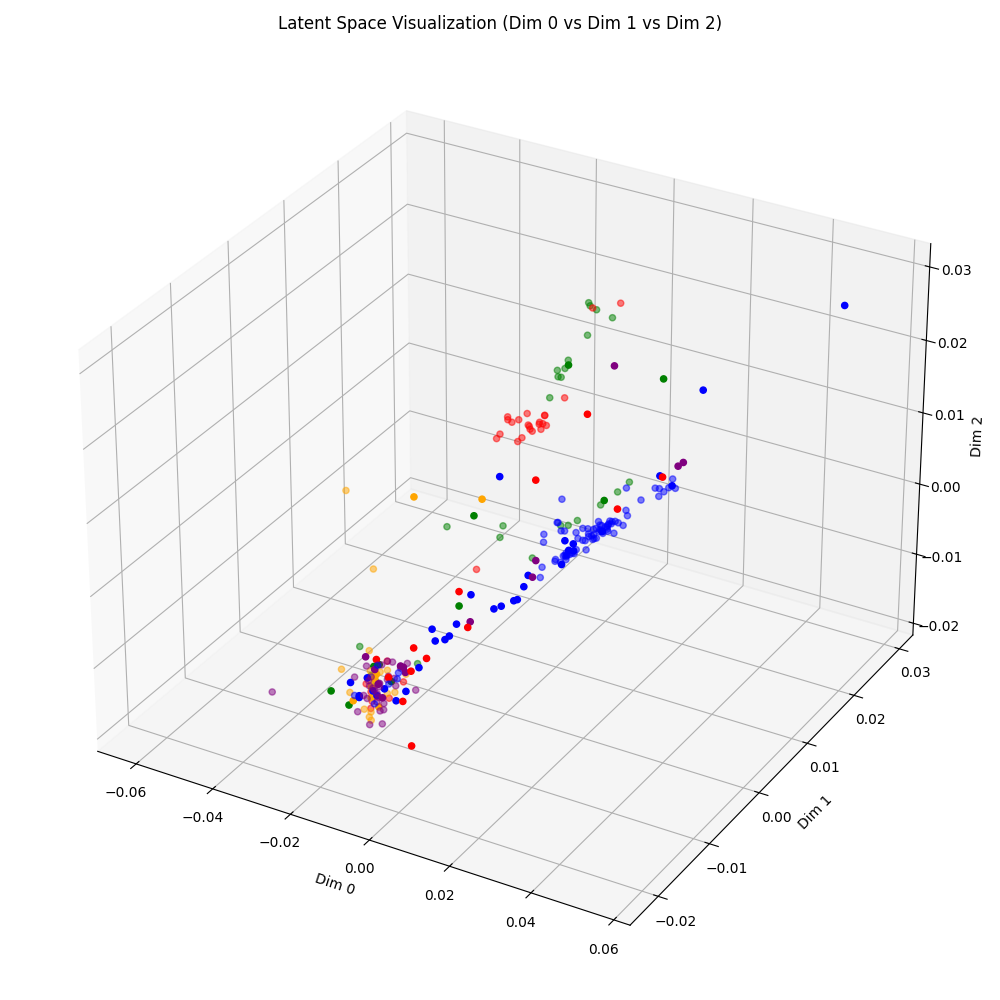
\includegraphics[width=\imgsize]{images/latent_space_viz_dataset_Worms.png}  \\ 

Step 0 & 
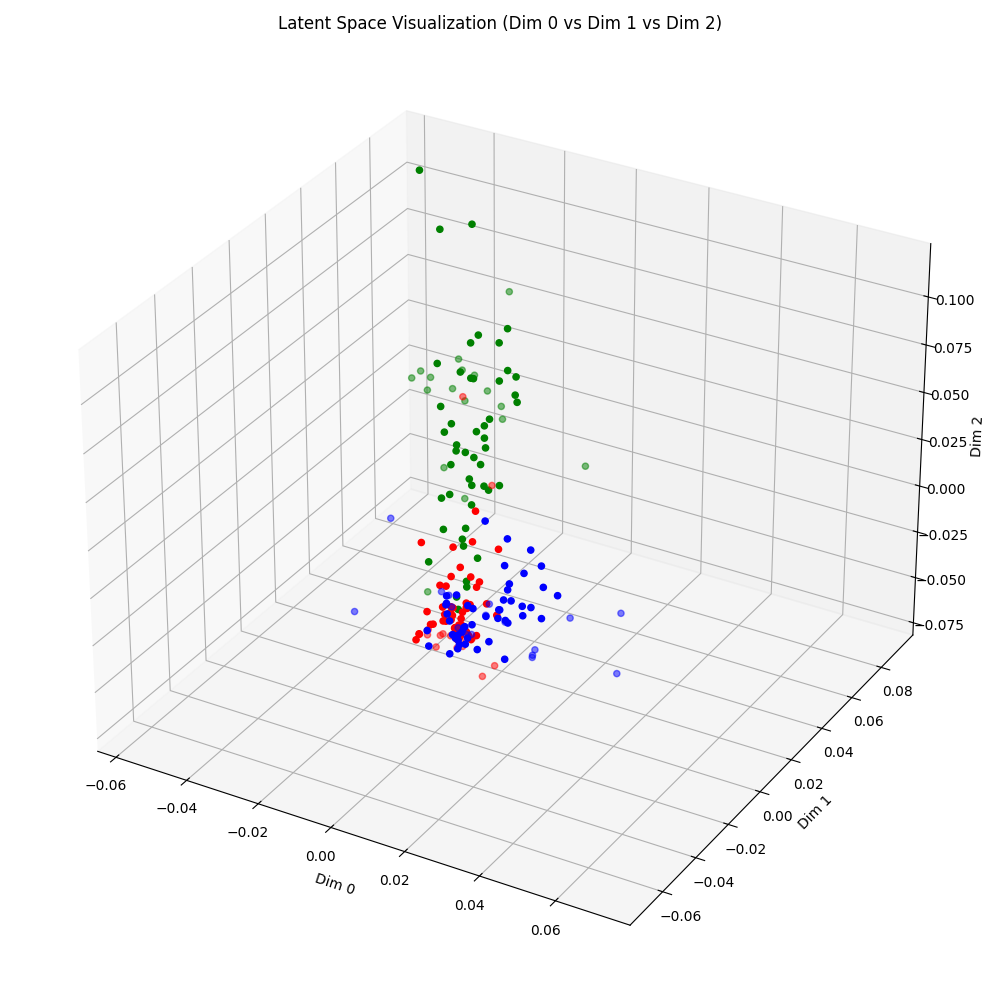
\includegraphics[width=\imgsize]{images/latent_space_viz_dataset_UMD_augmented_step_0.png} & 
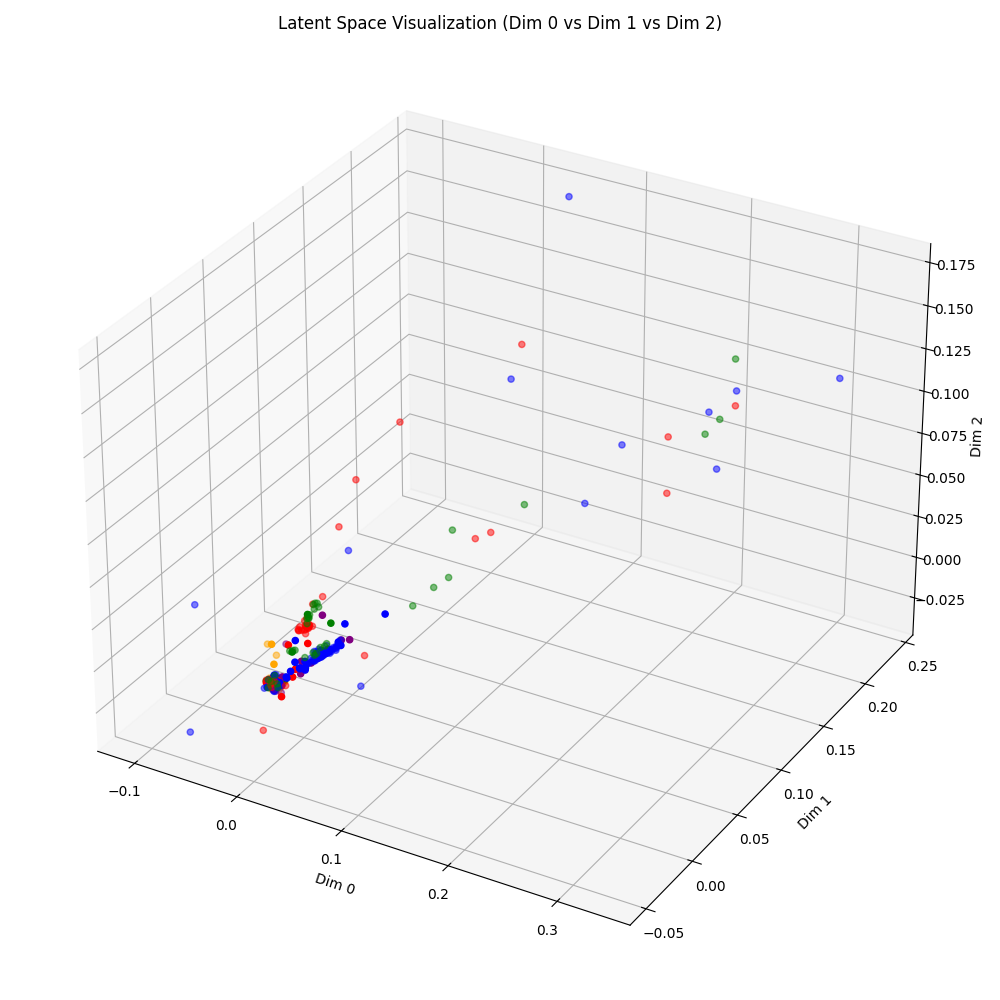
\includegraphics[width=\imgsize]{images/latent_space_viz_dataset_Worms_augmented_step_0.png} \\

Step 1 & 
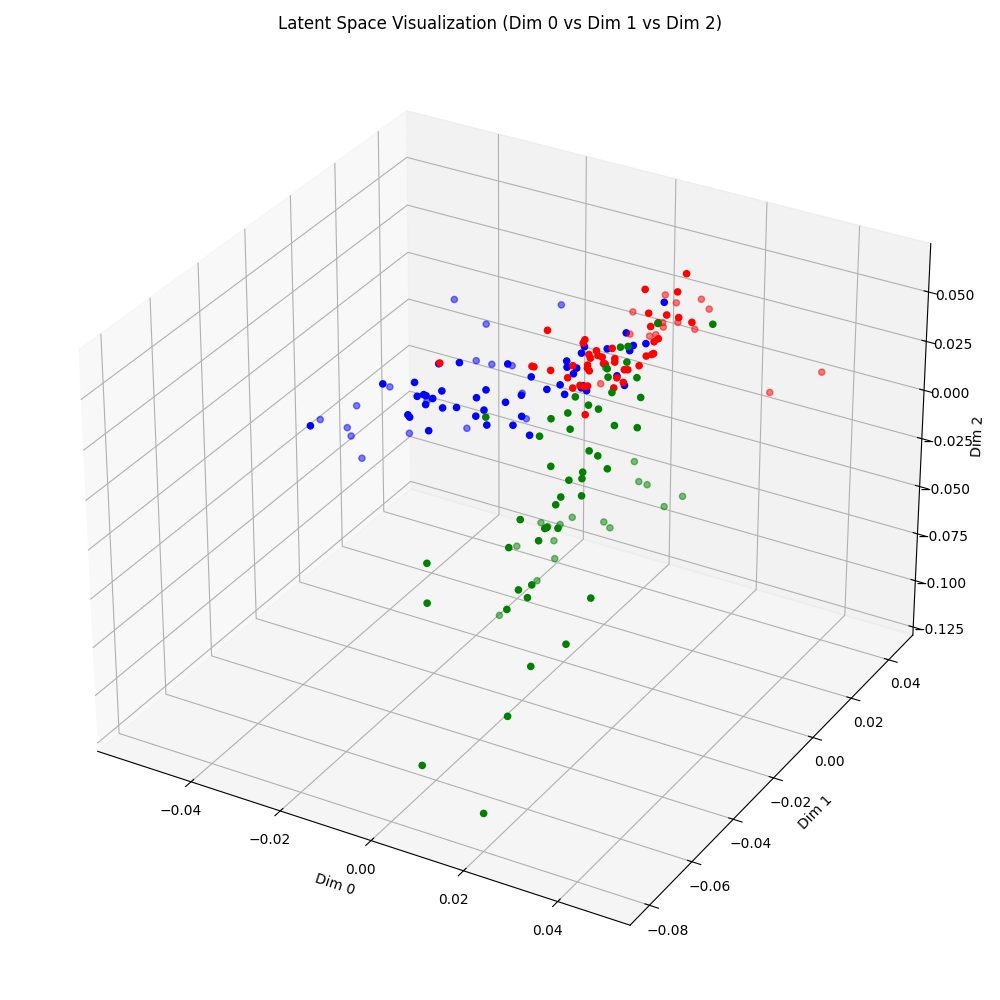
\includegraphics[width=\imgsize]{images/latent_space_viz_dataset_UMD_augmented_step_1.png} & 
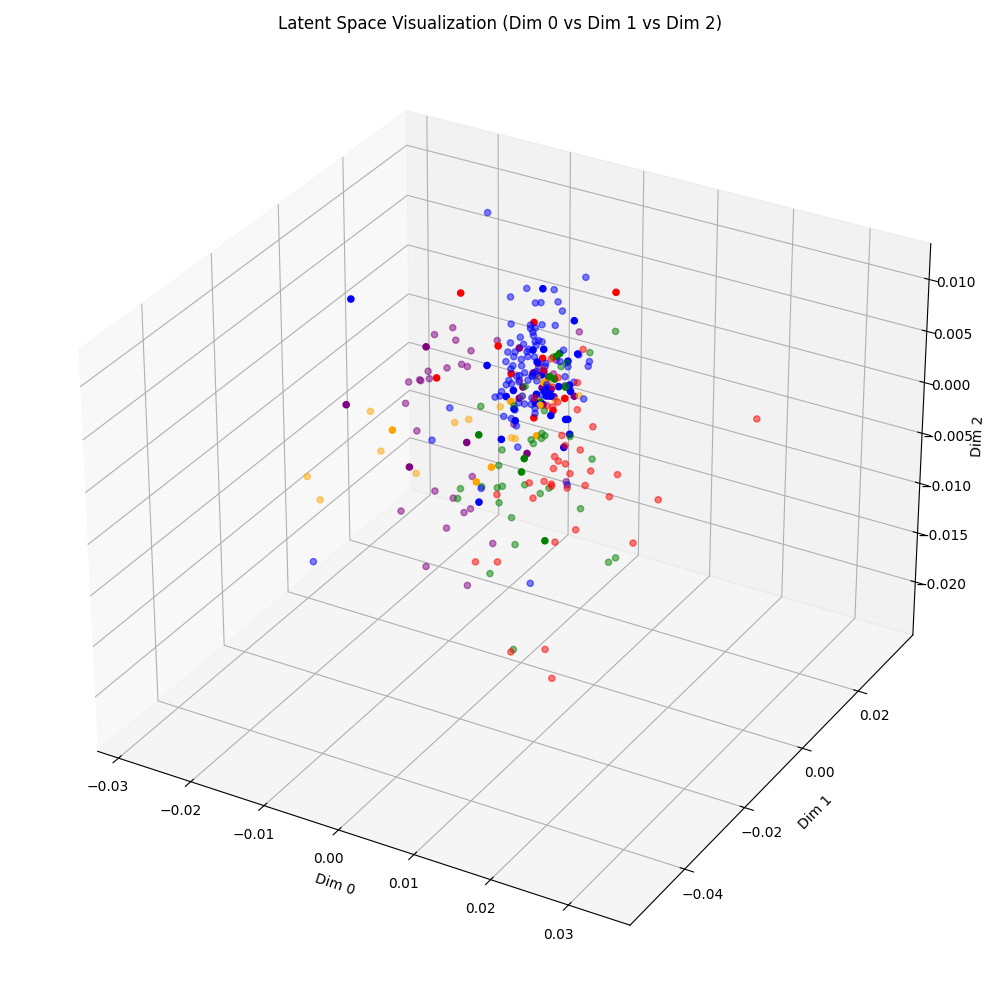
\includegraphics[width=\imgsize]{images/latent_space_viz_dataset_Worms_augmented_step_1.png}  \\ 

Step 2 & 
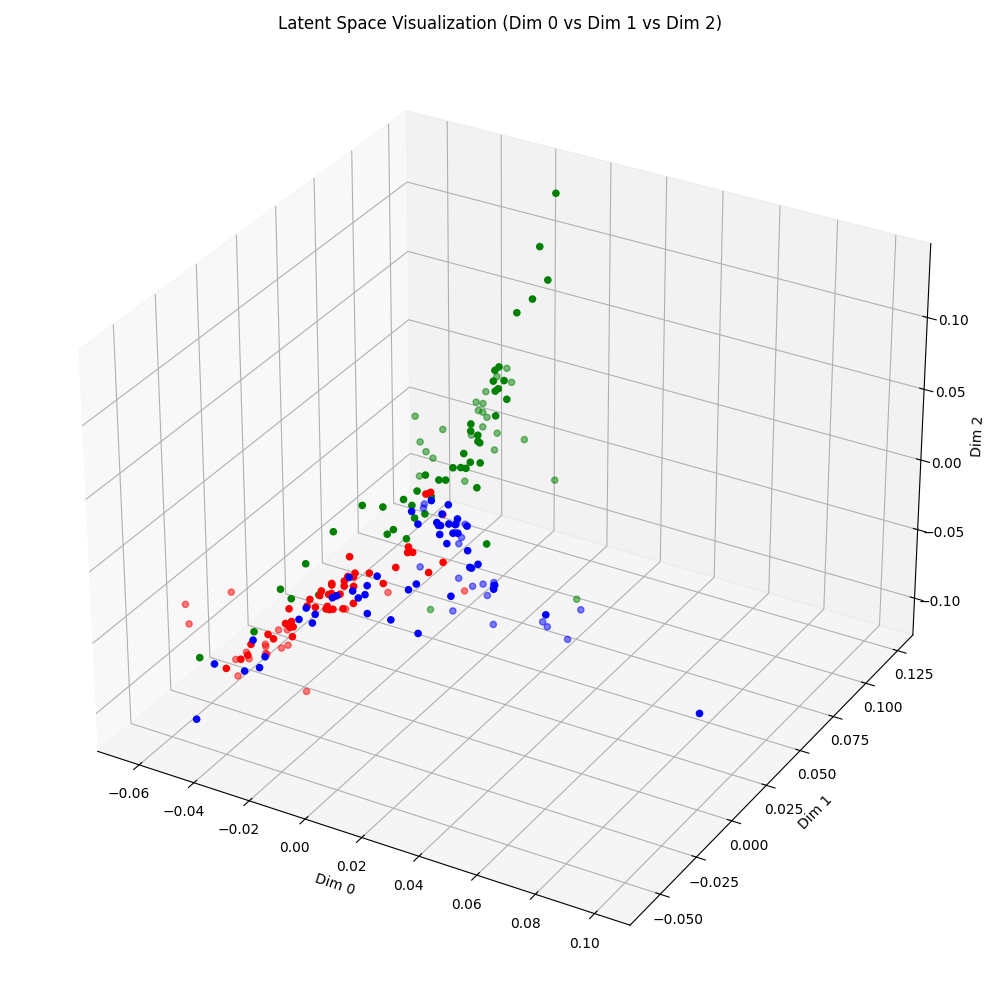
\includegraphics[width=\imgsize]{images/latent_space_viz_dataset_UMD_augmented_step_2.png} & 
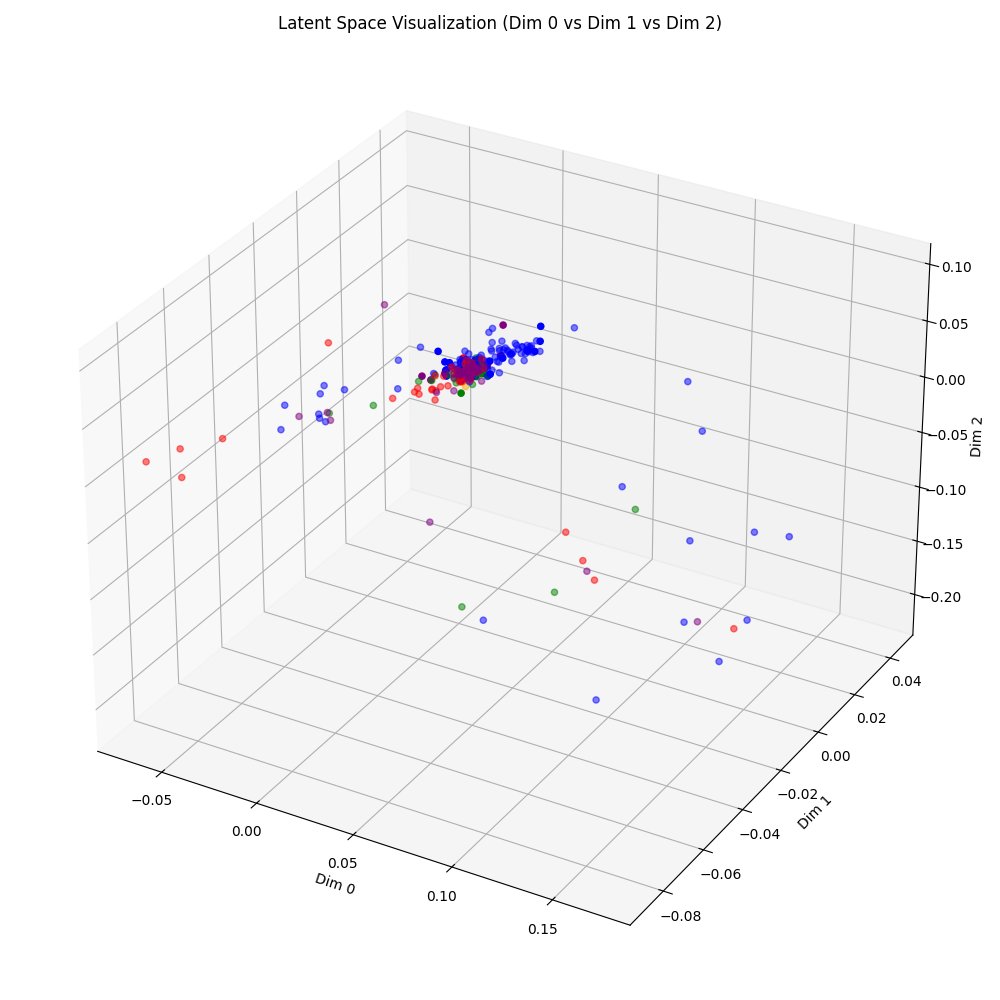
\includegraphics[width=\imgsize]{images/latent_space_viz_dataset_Worms_augmented_step_2.png}  \\ 

Step 3 & 
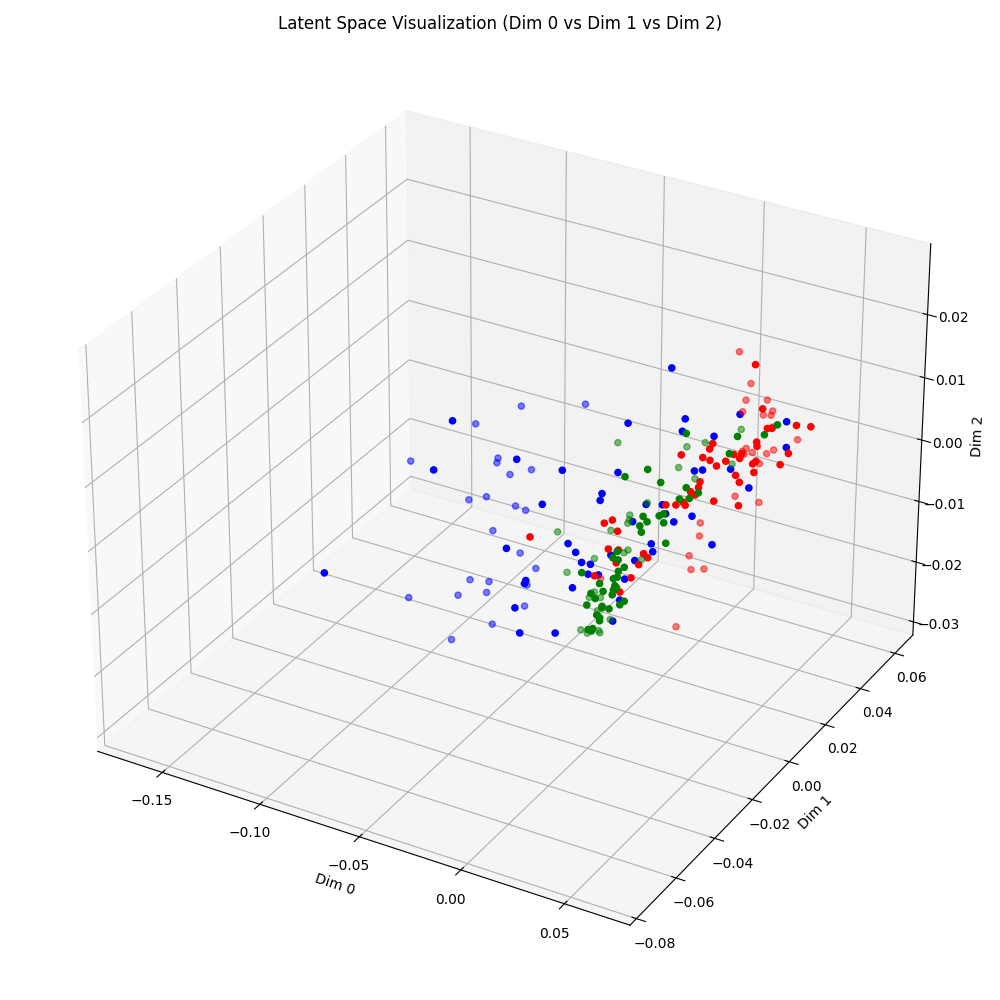
\includegraphics[width=\imgsize]{images/latent_space_viz_dataset_UMD_augmented_step_3.png} & 
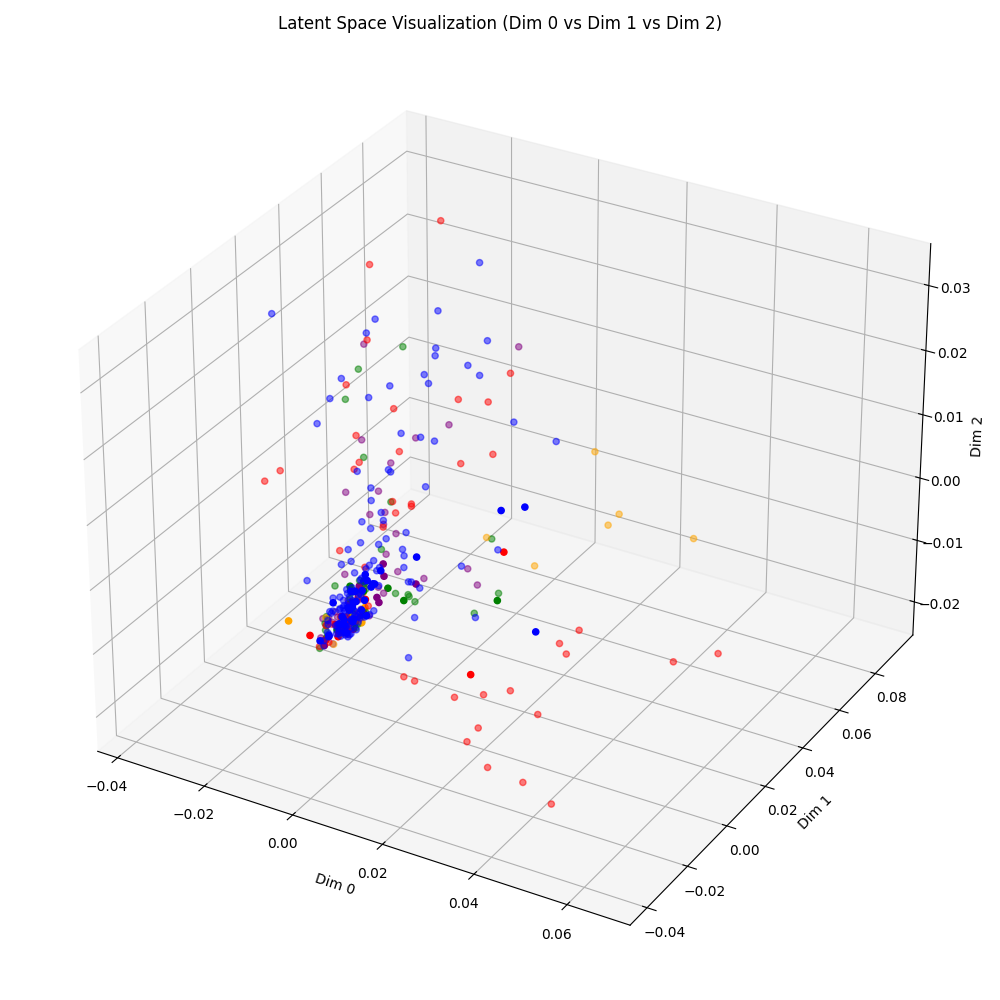
\includegraphics[width=\imgsize]{images/latent_space_viz_dataset_Worms_augmented_step_3.png} \\ 

Step 4 & 
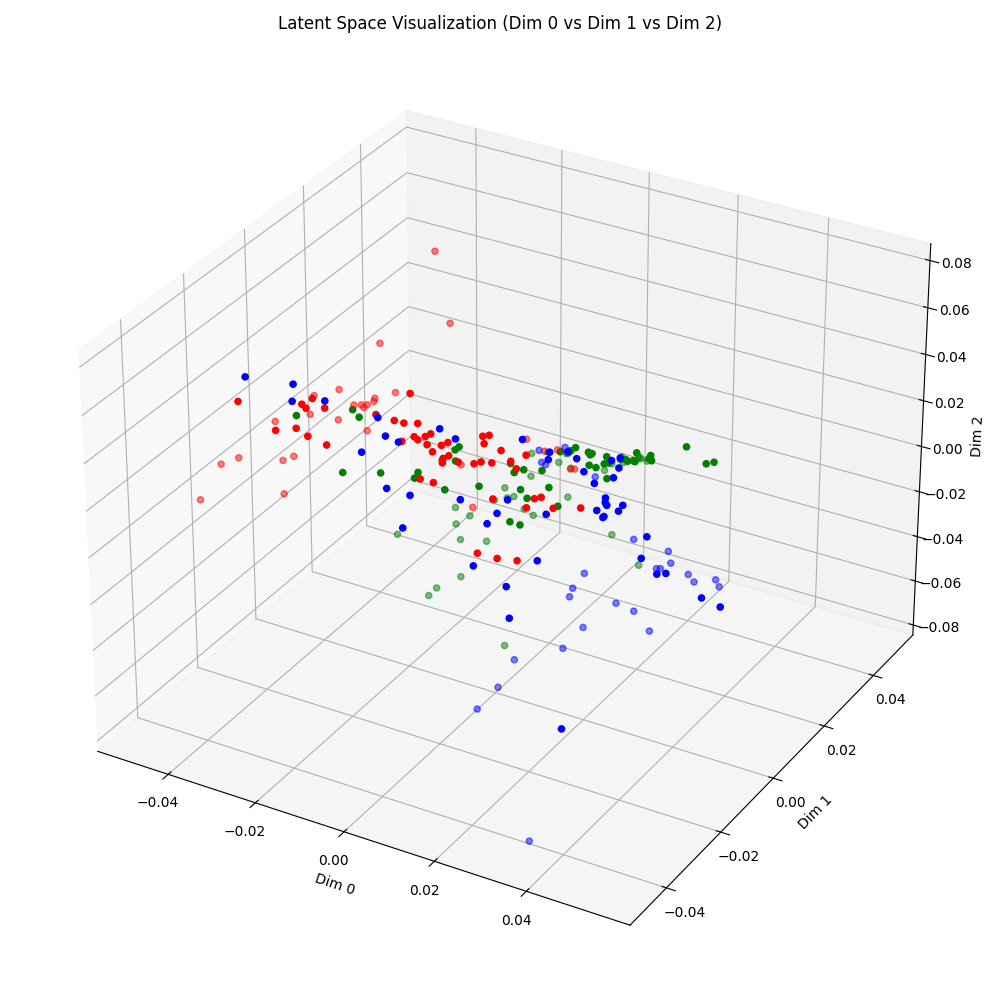
\includegraphics[width=\imgsize]{images/latent_space_viz_dataset_UMD_augmented_step_4.png} & 
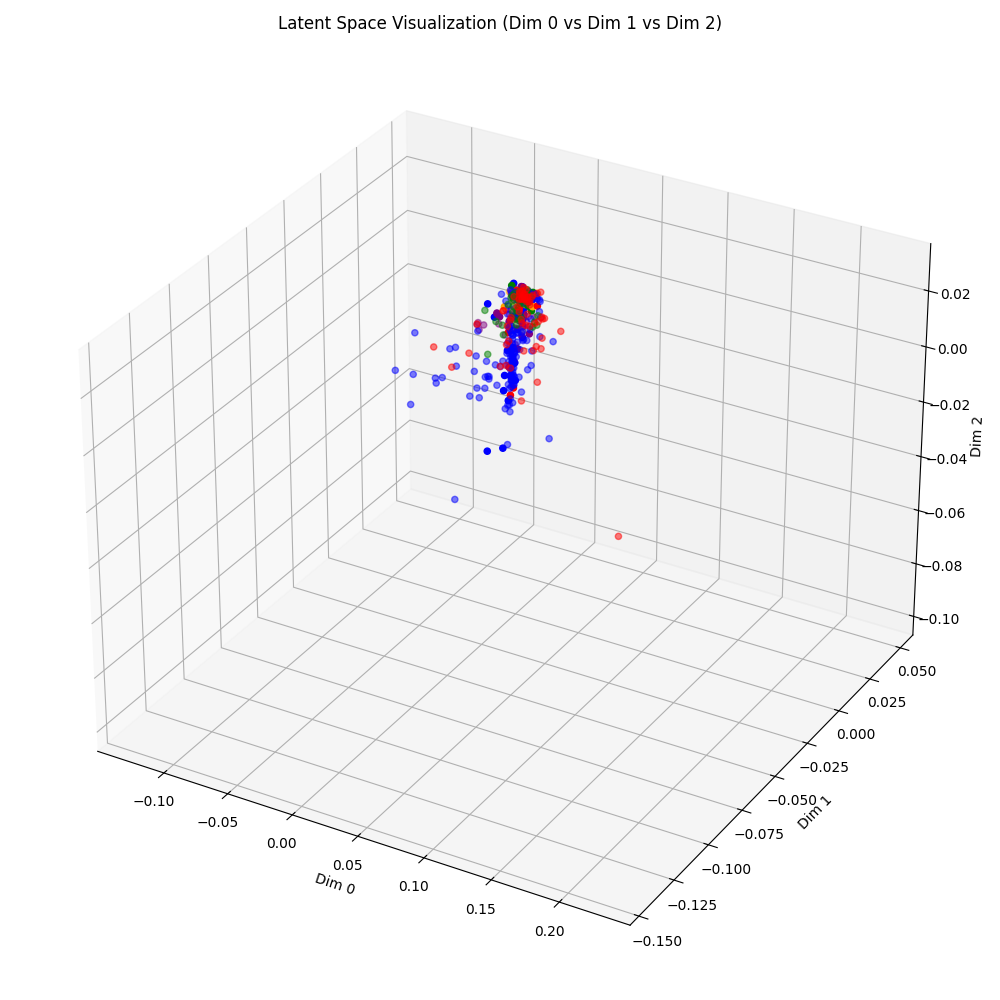
\includegraphics[width=\imgsize]{images/latent_space_viz_dataset_Worms_augmented_step_4.png} \\ 

Step 5 & 
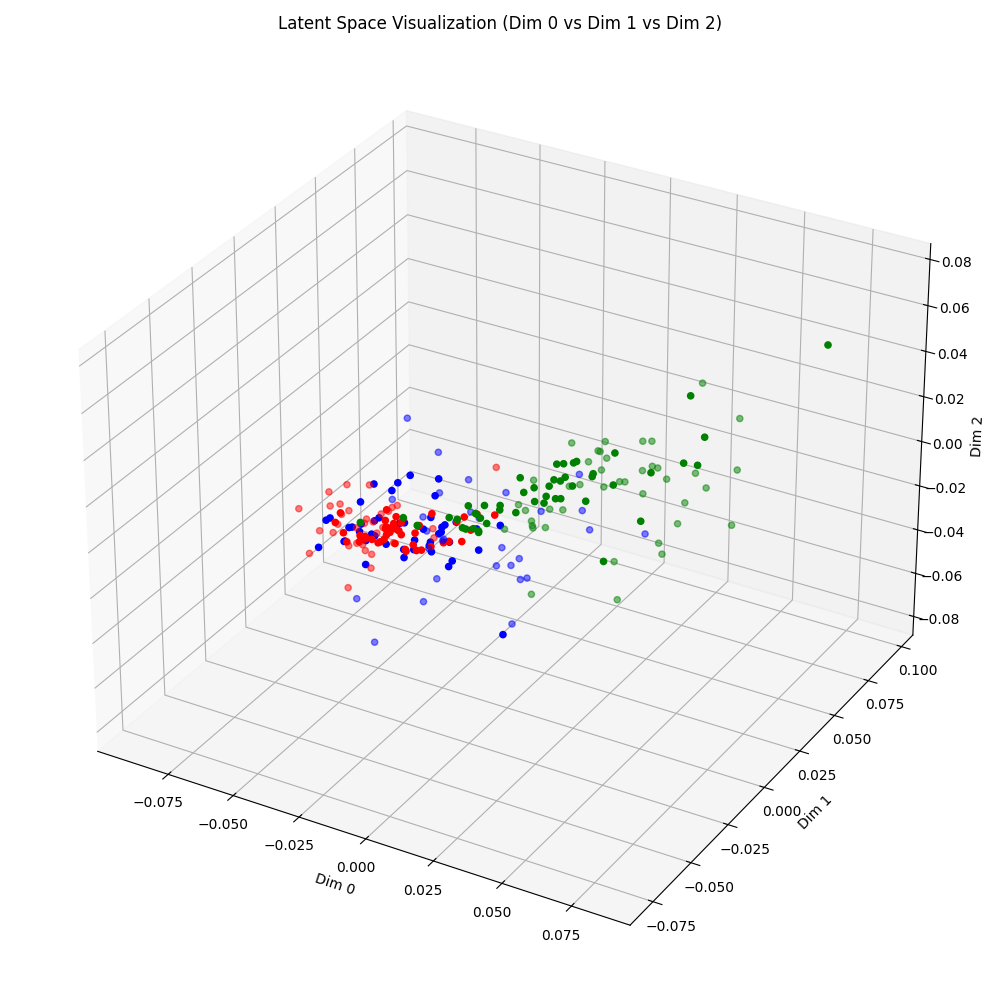
\includegraphics[width=\imgsize]{images/latent_space_viz_dataset_UMD_augmented_step_5.png} & 
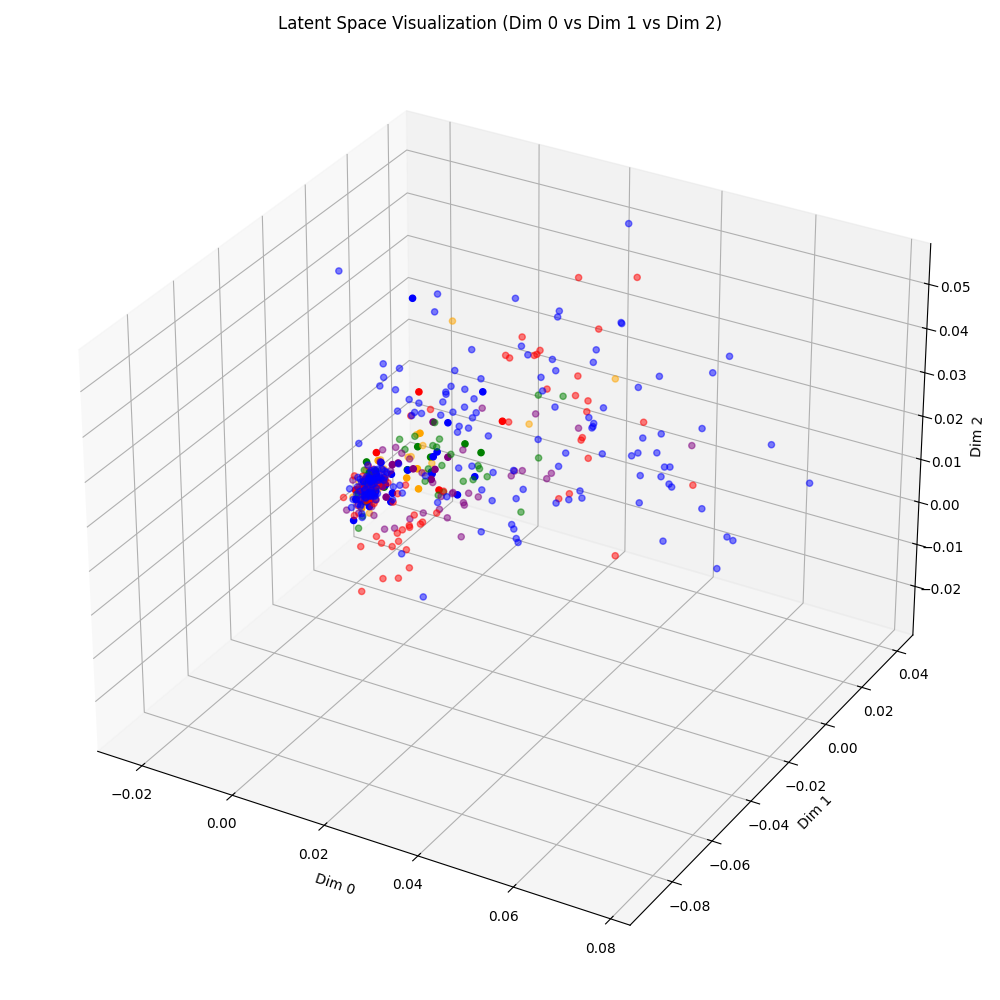
\includegraphics[width=\imgsize]{images/latent_space_viz_dataset_Worms_augmented_step_5.png}  \\ 
\bottomrule
\end{tabular}
%\caption{Latent Space Evolution: UMD, Worms}
\end{table*}
\fi  % --- end Appendix L ---



% \begin{table*}[p]
% \centering
%
% \caption{Discrepancy Metrics Across Datasets}
% \label{tab:discrepancy_metrics}
% \begin{tabular}{rlccc}
% \# &      Dataset &  Ratio &    Dispersion$_{TEST}$ &   Dispersion$_{TRAIN}$ \\
% \toprule
% D1 & ACSF1 & 0.96 & $1.01\times10^{3}$ & $1.04\times10^{3}$ \\
% D2 & Adiac & 1.09 & $2.81\times10^{1}$ & $2.25\times10^{1}$ \\
% D3 & ArrowHead & 1.16 & $1.71\times10^{0}$ & $1.88\times10^{0}$ \\
% D4 & BME & 1.13 & $1.64\times10^{2}$	&	$1.26\times10^{2}$\\
% D5 & Beef & 0.94 & $6.40\times10^{1}$ & $6.78\times10^{1}$ \\
% D6 & BeetleFly & 0.89 & $5.79\times10^{1}$ & $5.30\times10^{1}$ \\
% D7 & BirdChicken & 1.30 & $5.28\times10^{1}$ & $5.47\times10^{1}$ \\
% D8 & Car & 1.51 & $3.94\times10^{2}$ & $3.95\times10^{2}$ \\
% D9 & CBF & 1.09 & $6.69\times10^{4}$ & $8.63\times10^{4}$ \\
% D10 & ChlorineConcentration & 1.05 & $9.02\times10^{1}$ & $9.00\times10^{1}$ \\
% D11& CinCECGTorso & 1.24 & $1.41\times10^{1}$ & $1.40\times10^{1}$ \\
% D12 & Coffee & 1.07 & $8.05\times10^{0}$ & $8.45\times10^{0}$ \\
% D13& Computers & 0.97 & $1.94\times10^{2}$ & $1.98\times10^{2}$ \\
% D14 & Crop & 1.00 & $1.28\times10^{4}$ & $1.35\times10^{4}$ \\
% D15 & DistalPhalanxOutlineAgeGroup & 1.21 & $6.78\times10^{1}$ & $6.71\times10^{1}$ \\
% D16 & DistalPhalanxOutlineCorrect & 0.96 & $5.31\times10^{0}$ & $6.94\times10^{0}$ \\
% D17 & DistalPhalanxTW & 1.04 & $2.07\times10^{1}$ & $2.07\times10^{1}$ \\
% D18 & Earthquakes & 1.00 & $1.31\times10^{2}$ & $1.24\times10^{2}$ \\
% D19 & ECG200 & 1.21 & $1.28\times10^{2}$ & $1.25\times10^{2}$ \\
% D20 & ECG5000 & 1.19 & $4.17\times10^{1}$ & $4.77\times10^{1}$ \\
% D21 & ECGFiveDays & 1.01 & $5.42\times10^{1}$ & $4.85\times10^{1}$ \\
% D22 & ElectricDevices & 1.10 & $1.02\times10^{2}$ & $9.84\times10^{1}$ \\
% D23 & EOGHorizontalSignal & 1.18 & $3.01\times10^{1}$ & $2.65\times10^{1}$ \\
% D24 & EOGVerticalSignal & 0.77 & $6.38\times10^{3}$ & $5.62\times10^{3}$ \\
% D25& EthanolLevel & 0.87 & $3.18\times10^{1}$ & $2.10\times10^{1}$ \\
% D26 & FaceAll & 0.97 & $3.58\times10^{1}$ & $3.67\times10^{1}$ \\
% D27 & FaceFour & 1.04 & $5.44\times10^{1}$ & $5.14\times10^{1}$ \\
% D28 & FacesUCR & 1.12 & $1.20\times10^{3}$ & $1.08\times10^{3}$ \\
% D29 & Fish & 1.00 & $1.13\times10^{3}$ & $9.94\times10^{2}$ \\
% D30 & FordA & 0.99 & $3.73\times10^{3}$ & $3.83\times10^{3}$ \\
% D31 & FordB & 0.98 & $2.81\times10^{0}$ & $2.80\times10^{0}$ \\
% D32 & FreezerRegularTrain & 1.01 & $2.47\times10^{3}$ & $3.27\times10^{3}$ \\
% D33 & FreezerSmallTrain & 1.11 & $2.29\times10^{2}$ & $2.35\times10^{2}$ \\
% D34 & GunPoint & 1.04 & $3.83\times10^{2}$ & $3.91\times10^{2}$ \\
% D35 & GunPointAgeSpan & 1.00 & $5.50\times10^{0}$ & $4.90\times10^{0}$ \\
% D36 & GunPointMaleVersusFemale & 1.02 & $3.69\times10^{1}$ & $5.17\times10^{1}$ \\
% D37 & GunPointOldVersusYoung & 1.02 & $5.70\times10^{2}$ & $6.35\times10^{2}$ \\
% D38 & Ham & 1.07 & $4.23\times10^{2}$ & $3.75\times10^{2}$ \\
% D39 & HandOutlines & 0.46 & $1.50\times10^{2}$ & $1.39\times10^{2}$ \\
% D40 & Haptics & 1.08 & $3.27\times10^{1}$ & $2.98\times10^{1}$ \\
% D41 & Herring & 1.01 & $1.02\times10^{1}$ & $1.07\times10^{1}$ \\
% D42 & HouseTwenty & 0.99 & $2.44\times10^{0}$ & $2.79\times10^{0}$ \\
% D43 & InlineSkate & 1.07 & $8.25\times10^{0}$ & $6.80\times10^{0}$ \\
% D44 & InsectEPGRegularTrain & 1.26 & $1.88\times10^{1}$ & $1.94\times10^{1}$ \\
% D45 & InsectEPGSmallTrain & 1.10 & $1.63\times10^{2}$ & $1.64\times10^{2}$ \\
% D46 & InsectWingbeatSound & 1.06 & $7.54\times10^{2}$ & $7.85\times10^{2}$ \\
% D47 & ItalyPowerDemand & 0.95 & $2.75\times10^{0}$ & $2.92\times10^{0}$ \\
% D48 & LargeKitchenAppliances & 1.01 & $3.68\times10^{1}$ & $3.08\times10^{1}$ \\
% D49 & Lightning2 & 1.02 & $5.96\times10^{1}$ & $1.31\times10^{2}$ \\
% D50 & Lightning7 & 0.94 & $3.32\times10^{1}$ & $3.80\times10^{1}$ \\
% D51 & Mallat & 1.11 & $2.40\times10^{1}$ & $2.32\times10^{1}$ \\
% D52 & Meat & 0.94 & $2.80\times10^{3}$ & $1.35\times10^{3}$ \\
% D53 & MedicalImages & 1.00 & $7.57\times10^{1}$ & $8.10\times10^{1}$ \\

% \bottomrule
% \end{tabular}
% \end{table*}

% \setcounter{table}{7}
% \begin{table*}[p]
% \centering
%  
% \caption{Discrepancy Metrics Across Datasets}
% \label{tab:discrepancy_metrics}
% \begin{tabular}{rlccc}
% \# &      Dataset &  Ratio &    Dispersion$_{TEST}$ &   Dispersion$_{TRAIN}$ \\
% \toprule
% D54 & MiddlePhalanxOutlineAgeGroup & 1.12 & $2.70\times10^{1}$ & $2.24\times10^{1}$ \\
% D55 & MiddlePhalanxOutlineCorrect & 0.77 & $1.01\times10^{6}$ & $1.02\times10^{6}$ \\
% D56 & MiddlePhalanxTW & 0.94 & $4.74\times10^{0}$ & $5.02\times10^{0}$ \\
% D57 & MixedShapesRegularTrain & 0.98 & $4.20\times10^{2}$ & $4.76\times10^{2}$ \\
% D58 & MixedShapesSmallTrain & 1.19 & $1.59\times10^{2}$ & $1.55\times10^{2}$ \\
% D59 & MoteStrain & 0.96 & $3.27\times10^{1}$ & $2.60\times10^{1}$ \\
% D60 & NonInvasiveFetalECGThorax1 & 0.98 & $1.31\times10^{2}$ & $1.33\times10^{2}$ \\
% D61 & NonInvasiveFetalECGThorax2 & 0.97 & $2.52\times10^{0}$ & $2.42\times10^{0}$ \\
% D62 & OliveOil & 0.91 & $5.64\times10^{0}$ & $5.94\times10^{0}$ \\
% D63 & OSULeaf & 0.98 & $8.85\times10^{3}$ & $6.43\times10^{3}$ \\
% D64 & PhalangesOutlinesCorrect & 0.95 & $2.02\times10^{1}$ & $2.00\times10^{1}$ \\
% D65 & Plane & 0.94 & $9.58\times10^{1}$ & $1.01\times10^{2}$ \\
% D66 & PowerCons & 1.02 & $2.07\times10^{4}$ & $1.63\times10^{4}$ \\
% D67 & ProximalPhalanxOutlineAgeGroup & 0.94 & $4.70\times10^{2}$ & $7.09\times10^{2}$ \\
% D68 & ProximalPhalanxOutlineCorrect & 0.87 & $1.34\times10^{1}$ & $1.48\times10^{1}$ \\
% D69 & ProximalPhalanxTW & 0.94 & $1.39\times10^{4}$ & $1.36\times10^{4}$ \\
% D70 & RefrigerationDevices & 1.05 & $4.23\times10^{1}$ & $4.01\times10^{1}$ \\
% D71 & Rock & 1.27 & $1.16\times10^{2}$ & $1.11\times10^{2}$ \\
% D72 & ScreenType & 0.88 & $2.18\times10^{2}$ & $2.46\times10^{2}$ \\
% D73 & SemgHandGenderCh2 & 0.97 & $1.47\times10^{2}$ & $1.53\times10^{2}$ \\
% D74 & SemgHandMovementCh2 & 1.00 & $1.23\times10^{4}$ & $1.24\times10^{4}$ \\
% D75 & SemgHandSubjectCh2 & 0.95 & $5.14\times10^{1}$ & $5.28\times10^{1}$ \\
% D76 & ShapeletSim & 1.14 & $1.41\times10^{4}$ & $1.46\times10^{4}$ \\
% D77 & ShapesAll & 0.94 & $4.40\times10^{1}$ & $3.95\times10^{1}$ \\
% D78 & SmallKitchenAppliances & 0.99 & $2.49\times10^{1}$ & $2.61\times10^{1}$ \\
% D79 & SmoothSubspace & 1.04 & $4.86\times10^{1}$ & $3.19\times10^{1}$ \\
% D80 & SonyAIBORobotSurface1 & 1.00 & $8.36\times10^{0}$ & $8.36\times10^{0}$ \\
% D81 & SonyAIBORobotSurface2 & 1.18 & $2.80\times10^{1}$ & $2.36\times10^{1}$ \\
% D82 & StarLightCurves & 1.05 & $5.40\times10^{4}$ & $4.59\times10^{4}$ \\
% D83 & Strawberry & 0.91 & $1.59\times10^{2}$ & $1.56\times10^{2}$ \\
% D84 & SwedishLeaf & 0.96 & $4.69\times10^{2}$ & $4.37\times10^{2}$ \\
% D85 & Symbols & 1.53 & $1.23\times10^{1}$ & $3.72\times10^{0}$ \\
% D86 & SyntheticControl & 1.02 & $2.29\times10^{2}$ & $1.92\times10^{2}$ \\
% D87 & ToeSegmentation1 & 1.18 & $2.19\times10^{2}$ & $2.16\times10^{2}$ \\
% D88 & ToeSegmentation2 & 0.97 & $2.03\times10^{2}$ & $1.72\times10^{2}$ \\
% D89 & Trace & 0.88 & $4.46\times10^{3}$ & $4.41\times10^{3}$ \\
% D90 & TwoLeadECG & 1.00 & $2.28\times10^{1}$ & $2.32\times10^{1}$ \\
% D91 & TwoPatterns & 1.00 & $5.83\times10^{2}$ & $3.90\times10^{2}$ \\
% D92 & UMD & 0.97 & $1.89\times10^{1}$ & $1.89\times10^{1}$ \\
% D93 & UWaveGestureLibraryAll & 1.04 & $5.73\times10^{1}$ & $5.46\times10^{1}$ \\
% D94 & UWaveGestureLibraryX & 1.02 & $6.81\times10^{1}$ & $6.67\times10^{1}$ \\
% D95 & UWaveGestureLibraryY & 1.05 & $2.00\times10^{1}$ & $1.73\times10^{1}$ \\
% D96 & UWaveGestureLibraryZ & 1.06 & $8.64\times10^{0}$ & $9.18\times10^{0}$ \\
% D97 & Wafer & 1.12 & $2.24\times10^{2}$ & $2.30\times10^{2}$ \\
% D98 & Wine & 0.87 & $3.34\times10^{4}$ & $3.33\times10^{4}$ \\
% D99 & WordSynonyms & 1.11 & $4.32\times10^{3}$ & $5.08\times10^{3}$ \\
% D100 & Worms & 0.89 & $1.13\times10^{2}$ & $1.00\times10^{2}$ \\
% D101& WormsTwoClass & 0.93 & $4.09\times10^{1}$ & $4.26\times10^{1}$ \\
% D102 & Yoga & 1.02 & $3.02\times10^{4}$ & $2.97\times10^{4}$ \\
% \bottomrule
% \end{tabular}
% \end{table*}